% !Mode:: "TeX:UTF-8"
% !TEX program = xelatex

%%%%%%%%%% Port for macOS %%%%%%%%%%%
% Modified: Qin Yubo

\def\usewhat{xelatex}
\documentclass[12pt,openany,twoside]{book}
% 如果你认为文中中文逗号样式过于难看,可在Overleaf中尝试以下命令
% \documentclass[12pt,openany,twoside,fontset=ubuntu]{book}
% 也可以在windows环境下尝试以下命令,但在windows下可能会引发加粗命令失效
% \documentclass[12pt,openany,twoside,fontset=windows]{book}



%强制目录页的第一页的页眉页脚样式
\AtBeginDocument{\addtocontents{toc}{\protect\thispagestyle{only_foot}}}
                                                     % 本科生毕业论文通常采用单页排版
% !Mode:: "TeX:UTF-8"
%  Authors: 张井   Jing Zhang: prayever@gmail.com     天津大学2010级管理与经济学部信息管理与信息系统专业硕士生
%           余蓝涛 Lantao Yu: lantaoyu1991@gmail.com  天津大学2008级精密仪器与光电子工程学院测控技术与仪器专业本科生

%%%%%%%%%% Package %%%%%%%%%%%%
% \usepackage{CJK}
\usepackage{lmodern}
\usepackage[T1]{fontenc}
\usepackage{graphicx}                       % 支持插图处理
% \usepackage[a4paper,text={146.4true mm,239.2 true mm},top= 26.2true mm,left=31.8 true mm,head=6true mm,headsep=6.5true mm,foot=16.5true mm]{geometry}
%                                             % 支持版面尺寸设置
                                            
\usepackage[paper=a4paper,text={146.6mm,244.1mm},top= 27.5mm,left=35.7mm,head=6mm,headsep=6.5mm,foot=7.9mm]{geometry}
                                            % 支持版面尺寸设置
                                            
\usepackage[squaren]{SIunits}               % 支持国际标准单位

% \usepackage{algorithm}						%伪代码模板
% \usepackage{algorithmic}                    %伪代码模板

\usepackage{titlesec}                       % 控制标题的宏包
\usepackage{titletoc}                       % 控制目录的宏包
\usepackage{fancyhdr}                       % fancyhdr宏包 支持页眉和页脚的相关定义
\usepackage[UTF8]{ctex}                           % 支持中文显示

% \usepackage{CJKpunct}                       % 精细调整中文的标点符号
% \usepackage{color}                          % 支持彩色
\usepackage{amsmath}                        % AMSLaTeX宏包 用来排出更加漂亮的公式
\usepackage{amssymb}                        % 数学符号生成命令
\usepackage[below]{placeins}    %允许上一个section的浮动图形出现在下一个section的开始部分,还提供\FloatBarrier命令,使所有未处理的浮动图形立即被处理
\usepackage{multirow}                       % 使用Multirow宏包,使得表格可以合并多个row格
\usepackage{booktabs}                       % 表格,横的粗线;\specialrule{1pt}{0pt}{0pt}
\usepackage{longtable}                      % 支持跨页的表格。
\usepackage{tabularx}                       % 自动设置表格的列宽
\usepackage{subfigure}                      % 支持子图 %centerlast 设置最后一行是否居中
\usepackage[subfigure]{ccaption}            % 支持子图的中文标题
\usepackage[sort&compress,numbers]{natbib}  % 支持引用缩写的宏包
\usepackage{enumitem}                       % 使用enumitem宏包,改变列表项的格式
\usepackage{calc}                           % 长度可以用+ - * / 进行计算
\usepackage{txfonts}                        % 字体宏包
\usepackage{bm}                             % 处理数学公式中的黑斜体的宏包
\usepackage[amsmath,thmmarks,hyperref]{ntheorem}  % 定理类环境宏包,其中 amsmath 选项用来兼容 AMS LaTeX 的宏包

%\usepackage{CJKnumb}                        % 提供将阿拉伯数字转换成中文数字的命令
\usepackage{indentfirst}                    % 首行缩进宏包
% \usepackage{CJKutf8}                        % 用在UTF8编码环境下,它可以自动调用CJK,同时针对UTF8编码作了设置
%\usepackage{hypbmsec}                      % 用来控制书签中标题显示内容
\newcommand{\tabincell}[2]{\begin{tabular}{@{}#1@{}}#2\end{tabular}}
\usepackage{xcolor}
\usepackage{threeparttable}                 %支持对表格中的数据进行注释
%支持代码环境
\usepackage{listings}
\lstset{numbers=left,
language=[ANSI]{C},
numberstyle=\tiny,
extendedchars=false,
showstringspaces=false,
breakatwhitespace=false,
breaklines=true,
captionpos=b,
keywordstyle=\color{blue!70},
commentstyle=\color{red!50!green!50!blue!50},
frame=shadowbox,
rulesepcolor=\color{red!20!green!20!blue!20}
}
%支持算法环境
% \usepackage[boxed,ruled,lined]{algorithm2e}
%\usepackage{algorithm2e}
\usepackage{algorithm}
\usepackage{algorithmic}
\usepackage{diagbox}

\usepackage{bbm}
\usepackage{array}
\newcommand{\PreserveBackslash}[1]{\let\temp=\\#1\let\\=\temp}
\newcolumntype{C}[1]{>{\PreserveBackslash\centering}p{#1}}
\newcolumntype{R}[1]{>{\PreserveBackslash\raggedleft}p{#1}}
\newcolumntype{L}[1]{>{\PreserveBackslash\raggedright}p{#1}}

\def\atemp{xelatex}\ifx\atemp\usewhat
\usepackage[unicode,
            pdfstartview=FitH,
            bookmarksnumbered=true,
            bookmarksopen=true,
            colorlinks=true,   % false会出现红框,true文字就是链接
            pdfborder={0 0 1},
            citecolor=black,
            linkcolor=black,    %链接字颜色
            anchorcolor=black,
            urlcolor=black,
            breaklinks=true
            ]{hyperref}
\fi

                                % 定义本文所使用宏包
\graphicspath{{figures/}}                            % 定义所有的图像文件在 figures 子目录下
\begin{document}                                     % 开始全文
% !Mode:: "TeX:UTF-8"
%  Authors: 张井   Jing Zhang: prayever@gmail.com     天津大学2010级管理与经济学部信息管理与信息系统专业硕士生
%           余蓝涛 Lantao Yu: lantaoyu1991@gmail.com  天津大学2008级精密仪器与光电子工程学院测控技术与仪器专业本科生

%%%%%%%%%% Fonts Definition and Basics %%%%%%%%%%%%%%%%%
\newcommand{\song}{\songti}    % 宋体
\newcommand{\fs}{\fangsong}        % 仿宋体
\newcommand{\kai}{\kaishu}      % 楷体
\newcommand{\hei}{\heiti}      % 黑体
\newcommand{\li}{\lishu}        % 隶书
\newcommand{\kaiGB}{\CJKfamily{kai}}      % 楷体GB2312, 用于独创性说明
\newcommand{\yihao}{\fontsize{26pt}{26pt}\selectfont}       % 一号, 1.倍行距
\newcommand{\xiaoyi}{\fontsize{24pt}{24pt}\selectfont}      % 小一, 1.倍行距
\newcommand{\erhao}{\fontsize{22pt}{1.25\baselineskip}\selectfont}       % 二号, 1.25倍行距
\newcommand{\xiaoer}{\fontsize{18pt}{18pt}\selectfont}      % 小二, 单倍行距
\newcommand{\sanhao}{\fontsize{16pt}{16pt}\selectfont}      % 三号, 1.倍行距
\newcommand{\xiaosan}{\fontsize{15pt}{15pt}\selectfont}     % 小三, 1.倍行距
\newcommand{\sihao}{\fontsize{14pt}{14pt}\selectfont}       % 四号, 1.0倍行距
\newcommand{\xiaosi}{\fontsize{12pt}{20pt}\selectfont}      % 小四, 1.倍行距
\newcommand{\wuhao}{\fontsize{10.5pt}{10.5pt}\selectfont}   % 五号, 单倍行距
\newcommand{\xiaowu}{\fontsize{9pt}{9pt}\selectfont}        % 小五, 单倍行距

\setmainfont{Times New Roman}

%\CJKcaption{gb_452}
%\CJKtilde  % 重新定义了波浪符~的意义
\newcommand\prechaptername{第}
\newcommand\postchaptername{章}

% 调整罗列环境的布局
\setitemize{leftmargin=3em,itemsep=0em,partopsep=0em,parsep=0em,topsep=-0em}
\setenumerate{leftmargin=3em,itemsep=0em,partopsep=0em,parsep=0em,topsep=0em}
%\setlength{\baselineskip}{20pt}
%\renewcommand{\baselinestretch}{1.38} % 设置行距

%避免宏包 hyperref 和 arydshln 不兼容带来的目录链接失效的问题。
\def\temp{\relax}
\let\temp\addcontentsline
\gdef\addcontentsline{\phantomsection\temp}

% 自定义项目列表标签及格式 \begin{publist} 列表项 \end{publist}
\newcounter{pubctr} %自定义新计数器
\newenvironment{publist}{%%%%%定义新环境
\begin{list}{[\arabic{pubctr}]} %%标签格式
    {
     \usecounter{pubctr}
     \setlength{\leftmargin}{2.5em}     % 左边界 \leftmargin =\itemindent + \labelwidth + \labelsep
     \setlength{\itemindent}{0em}     % 标号缩进量
     \setlength{\labelsep}{1em}       % 标号和列表项之间的距离,默认0.5em
     \setlength{\rightmargin}{0em}    % 右边界
     \setlength{\topsep}{0ex}         % 列表到上下文的垂直距离
     \setlength{\parsep}{0ex}         % 段落间距
     \setlength{\itemsep}{0ex}        % 标签间距
     \setlength{\listparindent}{0pt} % 段落缩进量
    }}
{\end{list}}%%%%%

\makeatletter
\renewcommand\normalsize{
  \@setfontsize\normalsize{12pt}{12pt} % 小四对应12pt
  \setlength\abovedisplayskip{4pt}
  \setlength\abovedisplayshortskip{4pt}
  \setlength\belowdisplayskip{\abovedisplayskip}
  \setlength\belowdisplayshortskip{\abovedisplayshortskip}
  \setlength{\baselineskip}{20pt} % 设置固定行间距为20pt
  \let\@listi\@listI}
\def\defaultfont{\renewcommand{\baselinestretch}{1.0}\normalsize\selectfont}
% 设置行距和段落间垂直距离
\renewcommand{\CJKglue}{\hskip -0.08pt plus 0.08\baselineskip} % 每行大概35个字符

\makeatother
%%%%%%%%%%%%% Contents %%%%%%%%%%%%%%%%% 目录样式修改,(天津大学关于博士、硕士学位论文统一格式的规定 2016.10.24)


\renewcommand{\contentsname}{目\qquad 录}
\setcounter{tocdepth}{2}
\titlecontents{chapter}[0em]{\vspace{0pt}\xiaosi\song}%
             {\prechaptername\thecontentslabel\postchaptername\quad}{} %
             {\hspace{.5em}\titlerule*[7pt]{.}\xiaosi\contentspage}
\titlecontents{section}[2em]{\vspace{0pt}\xiaosi\song} %
            {\thecontentslabel\quad}{} %
            {\hspace{.5em}\titlerule*[7pt]{.}\xiaosi\contentspage}
\titlecontents{subsection}[4em]{\vspace{0pt}\xiaosi\song} %
            {\thecontentslabel\quad}{} %
            {\hspace{.5em}\titlerule*[7pt]{.}\xiaosi\contentspage}
%\titlecontents{subsubsection}[6em]{\vspace{0pt}\xiaosi\song} %
%            {\thecontentslabel\quad}{} %
%            {\hspace{.5em}\titlerule*[7pt]{.}\xiaosi\contentspage}

%%%%%%%%%% Chapter and Section %%%%%%%%%%%%%%%%% 各级标题样式((天津大学关于博士、硕士学位论文统一格式的规定 2016.10.24))
\setcounter{secnumdepth}{4}
\setlength{\parindent}{2em}
\renewcommand{\chaptername}{\prechaptername\thechapter\postchaptername}
\titleformat{\chapter}{\centering\xiaosan\hei}{\chaptername}{1em}{}
\titlespacing{\chapter}{0pt}{33pt}{33pt}
\titleformat{\section}{\sihao\hei}{\thesection}{1em}{}
\titlespacing{\section}{0pt}{21pt}{21pt}
\titleformat{\subsection}{\sihao\hei}{\thesubsection}{1em}{}
\titlespacing{\subsection}{0pt}{13pt}{13pt}
\titleformat{\subsubsection}{\xiaosi\hei}{\thesubsubsection}{1em}{}
\titlespacing{\subsubsection}{0pt}{10pt}{10pt}

%%%%%%%%%% Table, Figure and Equation %%%%%%%%%%%%%%%%%
\renewcommand{\tablename}{表} % 插表题头
\renewcommand{\figurename}{图} % 插图题头
\renewcommand{\thefigure}{\arabic{chapter}-\arabic{figure}} % 使图编号为 7-1 的格式 %\protect{~}
\renewcommand{\thetable}{\arabic{chapter}-\arabic{table}}%使表编号为 7-1 的格式
\renewcommand{\theequation}{\arabic{chapter}-\arabic{equation}}%使公式编号为 7-1 的格式
\renewcommand{\thesubfigure}{(\alph{subfigure})}%使子图编号为 (a)的格式
\renewcommand{\thesubtable}{(\alph{subtable})} %使子表编号为 (a)的格式
\makeatletter
\renewcommand{\p@subfigure}{\thefigure~} %使子图引用为 7-1 a) 的格式,母图编号和子图编号之间用~加一个空格
\makeatother

\renewcommand{\arraystretch}{1.7}   % 扩大表格行距,以近似达到垂直居中
\setlength{\abovecaptionskip}{5pt}  % 图标标题文字与图或表之间的间隔
\setlength{\belowcaptionskip}{5pt}
%% 定制浮动图形和表格标题样式
\makeatletter
\long\def\@makecaption#1#2{%
   \vskip\abovecaptionskip
   \sbox\@tempboxa{\centering\wuhao\song{#1\qquad #2} }%
   \ifdim \wd\@tempboxa >\hsize
     \centering\wuhao\song{#1\qquad #2} \par
   \else
     \global \@minipagefalse
     \hb@xt@\hsize{\hfil\box\@tempboxa\hfil}%
   \fi
   \vskip\belowcaptionskip}
\makeatother
\captiondelim{~~~~} %用来控制longtable表头分隔符

%%%%%%%%%% Theorem Environment %%%%%%%%%%%%%%%%%
\theoremstyle{plain}
\theorembodyfont{\song\rmfamily}
\theoremheaderfont{\hei\rmfamily}
\newtheorem{theorem}{定理~}[chapter]
\newtheorem{lemma}{引理~}[chapter]
\newtheorem{axiom}{公理~}[chapter]
\newtheorem{proposition}{命题~}[chapter]
\newtheorem{corollary}{推论~}[chapter]
\newtheorem{definition}{定义~}[chapter]
\newtheorem{conjecture}{猜想~}[chapter]
\newtheorem{example}{例~}[chapter]
\newtheorem{remark}{注~}[chapter]
% \newtheorem{algorithm}{算法~}[chapter]
\newenvironment{proof}{\noindent{\hei 证明:}}{\hfill $ \square $ \vskip 4mm}
\theoremsymbol{$\square$}

%%%%%%%%%% Page: number, header and footer  %%%%%%%%%%%%%%%%%

%\frontmatter 或 \pagenumbering{roman}
%\mainmatter 或 \pagenumbering{arabic}
\makeatletter
\renewcommand\frontmatter{\clearpage
  \@mainmatterfalse
  \pagenumbering{Roman}} % 正文前罗马字体编号
\makeatother

%%%%%%%%%% References %%%%%%%%%%%%%%%%%
\renewcommand{\bibname}{参考文献}
% 重定义参考文献样式,来自thu
\makeatletter
\renewenvironment{thebibliography}[1]{%
   \chapter*{\bibname}%
   \xiaosi
   \list{\@biblabel{\@arabic\c@enumiv}}%
        {\renewcommand{\makelabel}[1]{##1\hfill}
         \setlength{\baselineskip}{17pt}
         \settowidth\labelwidth{0.5cm}
         \setlength{\labelsep}{0pt}
         \setlength{\itemindent}{0pt}
         \setlength{\leftmargin}{\labelwidth+\labelsep}
         \addtolength{\itemsep}{-0.7em}
         \usecounter{enumiv}%
         \let\p@enumiv\@empty
         \renewcommand\theenumiv{\@arabic\c@enumiv}}%
    \sloppy\frenchspacing
    \clubpenalty4000%
    \@clubpenalty \clubpenalty
    \widowpenalty4000%
    \interlinepenalty4000%
    \sfcode`\.\@m}
   {\def\@noitemerr
     {\@latex@warning{Empty `thebibliography' environment}}%
    \endlist\frenchspacing}
\makeatother

\addtolength{\bibsep}{3pt} % 增加参考文献间的垂直间距
\setlength{\bibhang}{2em} %每个条目自第二行起缩进的距离

% 参考文献引用作为上标出现
%\newcommand{\citeup}[1]{\textsuperscript{\cite{#1}}}
\makeatletter
    \def\@cite#1#2{\textsuperscript{[{#1\if@tempswa , #2\fi}]}}
\makeatother
%% 引用格式
\bibpunct{[}{]}{,}{s}{}{,}

%%%%%%%%%% Cover %%%%%%%%%%%%%%%%%
% 封面、摘要、版权、致谢格式定义
\makeatletter
\def\ctitle#1{\def\@ctitle{#1}}\def\@ctitle{}
\def\etitle#1{\def\@etitle{#1}}\def\@etitle{}
\def\caffil#1{\def\@caffil{#1}}\def\@caffil{}
\def\cmacrosubject#1{\def\@cmacrosubject{#1}}\def\@cmacrosubject{}
\def\cmacrosubjecttitle#1{\def\@cmacrosubjecttitle{#1}}\def\@cmacrosubjecttitle{}
\def\csubject#1{\def\@csubject{#1}}\def\@csubject{}
\def\csubjecttitle#1{\def\@csubjecttitle{#1}}\def\@csubjecttitle{}
\def\cgrade#1{\def\@cgrade{#1}}\def\@cgrade{}
\def\cauthor#1{\def\@cauthor{#1}}\def\@cauthor{}
\def\cauthortitle#1{\def\@cauthortitle{#1}}\def\@cauthortitle{}
\def\csupervisor#1{\def\@csupervisor{#1}}\def\@csupervisor{}
\def\csupervisortitle#1{\def\@csupervisortitle{#1}}\def\@csupervisortitle{}
\def\cfirstsubject#1{\def\@cfirstsubject{#1}}\def\@cfirstsubject{}   % “一级学科”
\def\cfirstsubjecttitle#1{\def\@cfirstsubjecttitle{#1}}\def\@cfirstsubjecttitle{} % 一级学科名称
\def\teachertable#1{\def\@teachertable{#1}}\def\@teachertable{}  % 答辩老师表格
\def\cdate#1{\def\@cdate{#1}}\def\@cdate{}
\def\declaretitle#1{\def\@declaretitle{#1}}\def\@declaretitle{}
\def\declarecontent#1{\def\@declarecontent{#1}}\def\@declarecontent{}
\def\authorizationtitle#1{\def\@authorizationtitle{#1}}\def\@authorizationtitle{}
\def\authorizationcontent#1{\def\@authorizationcontent{#1}}\def\@authorizationconent{}
\def\authorizationadd#1{\def\@authorizationadd{#1}}\def\@authorizationadd{}
\def\authorsigncap#1{\def\@authorsigncap{#1}}\def\@authorsigncap{}
\def\supervisorsigncap#1{\def\@supervisorsigncap{#1}}\def\@supervisorsigncap{}
\def\signdatecap#1{\def\@signdatecap{#1}}\def\@signdatecap{}
\long\def\cabstract#1{\long\def\@cabstract{#1}}\long\def\@cabstract{}
\long\def\eabstract#1{\long\def\@eabstract{#1}}\long\def\@eabstract{}
\def\ckeywords#1{\def\@ckeywords{#1}}\def\@ckeywords{}
\def\ekeywords#1{\def\@ekeywords{#1}}\def\@ekeywords{}

%在book文件类别下,\leftmark自动存录各章之章名,\rightmark记录节标题
\pagestyle{fancy}
%去掉章节标题中的数字 务必放到\pagestyle{fancy}之后才会起作用
%%不要注销这一行,否则页眉会变成:“第1章1  绪论”样式
\renewcommand{\chaptermark}[1]{\markboth{\chaptername~\ #1}{}}
  \fancyhf{}
%   \fancyhead[C]{\song\wuhao \leftmark} % 页眉显示章节名称
  \fancyhead[CO]{\song\wuhao \leftmark}  % 奇数页,显示章标题
  \fancyhead[CE]{\song\wuhao 天津大学硕士学位论文} % 偶数页,显示“天津大学硕士学位论文”
  \fancyfoot[C]{\song\xiaowu ~\thepage~}
  \renewcommand{\headrulewidth}{0.7pt}%
  \renewcommand{\footrulewidth}{0pt}%

\fancypagestyle{plain}{% 设置开章页页眉页脚风格
    \fancyhf{}%
    \fancyhead[C]{\song\wuhao \leftmark}
    \fancyfoot[C]{\song\xiaowu ~\thepage~ } %%首页页脚格式
    \renewcommand{\headrulewidth}{0.7pt}%
    \renewcommand{\footrulewidth}{0pt}%
}

\fancypagestyle{only_foot}{% 设置摘要、目录的页眉页脚风格:无页眉((天津大学关于博士、硕士学位论文统一格式的规定 2016.10.24)貌似要这种only_foot的样式)
    \fancyhf{}%
    \fancyfoot[C]{\song\xiaowu ~\thepage~ }
    \renewcommand{\headrulewidth}{0pt}%
    \renewcommand{\footrulewidth}{0pt}%
}


\newlength{\@title@width}
\def\@put@covertitle#1{\makebox[\@title@width][s]{#1}}
% 定义封面
\def\makecover{
\clearpage{\pagestyle{empty}\cleardoublepage}
   \phantomsection
    \pdfbookmark[-1]{\@ctitle}{ctitle}

    \begin{titlepage}
      \vspace*{0.8cm}
      \begin{center}

      \vspace*{1cm}
      \begin{center}
      \renewcommand{\baselinestretch}{1.25} % 设置行距
      \song\erhao\textbf{\@ctitle} % 修改成宋体加粗 (天津大学关于博士、硕士学位论文统一格式的规定, 2016.10.24)
      \renewcommand{\baselinestretch}{1.25} % 设置行距
      \end{center}
      \vspace*{1cm}

    %  \vspace*{1cm}

      \begin{center}
      \renewcommand{\baselinestretch}{1.25} % 设置行距
      \song\erhao\textbf{\@etitle}  % 修改成宋体加粗1.25倍行距(英文默认变成了Times new Roman) (天津大学关于博士、硕士学位论文统一格式的规定, 2016.10.24)
      \renewcommand{\baselinestretch}{1.25} % 设置行距
      \end{center}

      \vspace*{1cm} %3cm
      \setlength{\@title@width}{4em}   % 影响“一级学科”的字间距
      {\song\xiaosi{
      \renewcommand{\arraystretch}{1}  % 此处修改行距,不影响正文中的表格行距
      \begin{tabular}{p{\@title@width}@{:}l}
        \@put@covertitle{\@cfirstsubjecttitle} & \@cfirstsubject \\
        \@put@covertitle{\@csubjecttitle} & \@csubject \\
        \@put@covertitle{\@cauthortitle} & \@cauthor \\
        \@put@covertitle{\@csupervisortitle} & \@csupervisor \\
      \end{tabular}
      }}
      
      \vspace*{1cm}
      {\@teachertable}


  \vspace*{1cm}
  \song\sihao\@caffil \\
  \song\sihao\@cdate

\end{center}
%  另起一页: 独创性声明和学位论文版权使用授权书
\newpage
    \clearpage{\pagestyle{empty}\cleardoublepage} %去除空白页的页眉页脚(由于每章从奇数页开始因此有空白页)
    \thispagestyle{empty} %去掉页眉页脚
    \vspace*{1cm}
    \renewcommand{\baselinestretch}{1} % 设置行距
    \begin{center}\song\xiaoer{\@declaretitle}\end{center}\par
    \vspace*{0.5cm}
    \song\xiaosi{\@declarecontent}\par
    \vspace*{1cm}
    {\song\xiaosi
    \@authorsigncap \makebox[2.5cm][s]{}
    \@signdatecap \makebox[2cm][s]{} 年 \makebox[1cm][s]{} 月 \makebox[1cm][s]{} 日
    }

    \vspace*{3cm}
    \begin{center}\song\xiaoer{\@authorizationtitle}\end{center}\par
    \vspace*{1cm}
    {
    \song\xiaosi{\@authorizationcontent}

    \@authorizationadd\par
    }

    \vspace*{2cm}
    {\song\xiaosi\setlength{\parindent}{-0.45em}
    \begin{tabularx}{\textwidth}{ll}
        \@authorsigncap \makebox[3.5cm][s]{}  & \@supervisorsigncap \makebox[3.5cm][s]{}   \\
         &  \\
        \@signdatecap \makebox[1.5cm][s]{} 年 \makebox[1cm][s]{} 月 \makebox[1cm][s]{} 日 &
         \@signdatecap \makebox[1.5cm][s]{} 年 \makebox[1cm][s]{} 月 \makebox[1cm][s]{} 日 \\
    \end{tabularx}
    }
\end{titlepage}

%%%%%%%%%%%%%%%%%%%   Abstract and Keywords  %%%%%%%%%%%%%%%%%%%%%%%
\clearpage{\pagestyle{empty}\cleardoublepage} %去除空白页的页眉页脚(由于每章从奇数页开始因此有空白页)
\markboth{摘~要}{摘~要}
\addcontentsline{toc}{chapter}{摘\qquad 要}
\chapter*{\centering\song\erhao\textbf{摘\qquad 要}}
\thispagestyle{only_foot}

\setcounter{page}{1}
\song\defaultfont
\@cabstract
\vspace{\baselineskip}

%\hangafter=1\hangindent=52.3pt\noindent   %如果取消该行注释,关键词换行时将会自动缩进
\noindent
{\song\sihao\textbf{ 关键词:}} \@ckeywords

%%%%%%%%%%%%%%%%%%%   English Abstract  %%%%%%%%%%%%%%%%%%%%%%%%%%%%%%
\clearpage{\pagestyle{empty}\cleardoublepage} %去除空白页的页眉页脚(由于每章从奇数页开始因此有空白页)
\markboth{ABSTRACT}{ABSTRACT}
\addcontentsline{toc}{chapter}{ABSTRACT}
\chapter*{\centering\erhao\textbf{ABSTRACT}}
\thispagestyle{only_foot}
\@eabstract
\vspace{\baselineskip}

%\hangafter=1\hangindent=60pt\noindent  %如果取消该行注释,KEY WORDS换行时将会自动缩进
\noindent
{\sihao\textbf{KEY WORDS:}}  \@ekeywords
}

\makeatother                       % 完成对论文各个部分格式的设置
\frontmatter                               % 以下是论文导言部分,包括论文的封面,中英文摘要和中文目录

\ctitle{基于深度学习脑电解码的智能脑机接口系统研究}  %封面用论文标题,自己可手动断行
\etitle{Research on Intelligent Brain-Computer Interface System based on Deep Learning EEG Signal Decoding}
\cfirstsubjecttitle{\textbf{一级学科}}
\cfirstsubject{\textbf{\underline{\makebox[14em][c]{}}}}   %专业
\csubjecttitle{\textbf{研究方向}}
\csubject{\textbf{\underline{\makebox[14em][c]{}}}}   %专业
\cauthortitle{\textbf{作者姓名}}     % 学位
\cauthor{\textbf{\underline{\makebox[14em][c]{}}}}   %学生姓名
\csupervisortitle{\textbf{指导教师}}
\csupervisor{\textbf{\underline{\makebox[14em][c]{}}}} %导师姓名

\teachertable{
\begin{table}[h]
\centering
\renewcommand{\arraystretch}{1}  % 临时定义一下行间距
\song\xiaosi{
\begin{tabularx}{\textwidth}{|*{4}{>{\centering\arraybackslash}X|}}
\hline
\textbf{答辩日期}                & \multicolumn{3}{c|}{2022年12月7日}       \\ \hline
\textbf{答辩委员会}               & \textbf{姓名} & \textbf{职称} & \textbf{工作单位} \\ \hline
\textbf{主席}                  &  &          &        \\ \hline
\multirow{2}{*}{\textbf{委员}} &       &      &     \\ \cline{2-4} 
                             &     \multirow{2}{*}{-} &     \multirow{2}{*}{-}&     \\ \hline
\end{tabularx}}
\end{table}}

\caffil{-} %学院名称
\cdate{\CJKdigits{\the\year} 年\CJKnumber{\the\month}  月 \CJKnumber{\the\day} 日}
% 如需改成二零一二年四月二十五日的格式,可以直接输入,即如下所示
\cdate{二〇二三年一月}
% \cdate{\the\year 年\the\month 月 \the\day 日} % 此日期显示格式为阿拉伯数字 如2012年4月25日


\declaretitle{独创性声明}
\declarecontent{
本人声明所呈交的学位论文是本人在导师指导下进行的研究工作和取得的研究成果,除了文中特别加以标注和致谢之处外,论文中不包含其他人已经发表或撰写过的研究成果,也不包含为获得 {\underline{\kaiGB{\sihao{\textbf{~~~~}}}}} 或其他教育机构的学位或证书而使用过的材料。与我一同工作的同志对本研究所做的任何贡献均已在论文中作了明确的说明并表示了谢意。
}
\authorizationtitle{学位论文版权使用授权书}
\authorizationcontent{
本学位论文作者完全了解{\underline{\kaiGB{\sihao{\textbf{~~--~~}}}}}有关保留、使用学位论文的规定。特授权{\underline{\kaiGB{\sihao{\textbf{~~--~~}}}}} 可以将学位论文的全部或部分内容编入有关数据库进行检索,并采用影印、缩印或扫描等复制手段保存、汇编以供查阅和借阅。同意学校向国家有关部门或机构送交论文的复印件和磁盘。
}
\authorizationadd{(保密的学位论文在解密后适用本授权说明)}
\authorsigncap{学位论文作者签名:}
\supervisorsigncap{导师签名:}
\signdatecap{签字日期:}

\cabstract{
脑机接口(BCI),作为人机交互的终极手段,在众多领域具有巨大的发展潜力。基于脑电图(EEG)的BCI系统由于其较低的使用成本和优秀的时间分辨率成为了辨识人脑状态和运动意图的有效手段之一。本课题设计了一套基于EEG的BCI系统——JS-AINS-40。该系统实现了对使用者EEG信号的采集,同时利用基于深度学习的辨识算法准确解码人脑状态与运动意图。

本课题设计的JS-AINS-40系统,通过采集模块实现对40通道EEG数据的同步采样,并经由下位机程序将EEG数据传输至上位机。上位机软件可以对数据进行实时保存、可视化以及类别标注。该系统具备高精度、高共模抑制比以及低噪声等优点,已通过医疗电气设备电磁兼容性检验,性能符合国家标准。

本课题设计的JS-AINS-40系统,针对具体的EEG数据范式分别设计了对应的解码算法。针对被动范式的情绪与疲劳EEG信号,引入结合自适应与早停机制的神经架构搜索(NAS)算法,成功解决当下面向被动范式EEG的深度学习模型设计复杂,调参耗时等问题。搜索得到的网络模型在公开情绪数据集,公开疲劳数据集以及基于JS-AINS-40系统自主采集的情绪数据集上分别得到82.96\%,84.63\%和78.50\%的分类辨识精度,在与其他先进算法的对比中极具竞争力。

针对主动范式中的运动想象EEG信号,引入由特征提取器、动态注意力模块和基于面向域分类器的迭代自训练策略组成的无监督域适应(UDA)框架。成功解决了由于该范式的EEG数据样本数量少,样本间差异大,不同想象动作脑区重叠所带来的模型辨识性能下降问题。使得BCI系统在同时跨被试、跨时段以及多想象类别的实际场景中的应用成为可能。在三个公开的运动想象数据集和基于JS-AINS-40系统自主采集的运动想象数据集上,该辨识算法分别取得了69.51\%、82.38\%,90.98\%以及70.08\%的辨识精度,成功击败了当前的最优模型。

所有的实验结果表明,本课题所设计的JS-AINS-40系统能够满足对于高质量脑电信号采集,人脑状态与意图解码的需求。

}
\ckeywords{脑机接口,脑电图,40导联脑电采集设备,深度学习技术,神经架构搜索,无监督域适应}

\eabstract{
Brain computer interface (BCI), the ultimate means of human-computer interaction, has excellent potential for development in many fields. Electroencephalography (EEG)-based BCI system has become one of the effective means for recognizing the states and motor intentions of the human brain, due to their low cost and excellent temporal resolution. The JS-AINS-40, an EEG-based BCI system, is designed to capture the EEG signal and translate the human brain intentions using deep learning-based recognition algorithms.

The JS-AINS-40 system is designed to synchronize the sampling of the 40 channels EEG data via the acquisition module and to transmit the data to the host computer. The data is saved, visualized and labeled in real time by the host computer software. The JS-AINS-40 system has the advantages of high precision, high common-mode rejection ratio and low noise, etc. It has passed the electromagnetic compatibility inspection of medical electrical equipment, and its performance is in line with national standards.

The JS-AINS-40 system designed in this project has corresponding decoding algorithms for different EEG data paradigms. Aiming at the emotion and fatigue EEG signals of the passive paradigm, the neural architecture search (NAS) algorithm combined with adaptive and early stop mechanism is introduced. It successfully solves the problems of complex design and time-consuming parameter adjustment of the current deep learning model. The networks obtained by searching get 82.96\%, 84.63\% and 78.50\% classification accuracy respectively on the public emotion dataset, the public fatigue dataset and the emotion dataset collected based on the JS-AINS-40 system. The final results are very competitive with other advanced algorithms.

An unsupervised domain adaptation (UDA) framework consisting of a feature extractor, a dynamic attention module and a domain-oriented classifier-based iterative self-training, is introduced for motor imagery EEG signals of active paradigm. It successfully solves the problem of model identification performance degradation caused by the small number of EEG samples in this paradigm, the large difference between features, and overlapping brain regions of different imagery movements. This framework makes it possible to apply the BCI system in real scenarios of simultaneous cross-subject, cross-time and multiple motor imagery categories. On three public motor imagery datasets and one dataset collected by JS-AINS 40 system, the proposed algorithm achieves 69.51\%, 82.38\%, 90.98\% and 70.08\% identification accuracy, which successfully beats the current optimal model.

All the experimental results show that the JS-AINS-40 system designed in this project can meet the requirements for high-quality EEG signal acquisition and decoding of the states or intentions of the human brain.

}

\ekeywords{Brain computer interface, Electroencephalography, 40-channel device for EEG signals recording, Deep learning technology, Neural architecture search, Unsupervised domain adaptation}


\makecover
\clearpage                      % 封面

%%%%%%%%%%   目录   %%%%%%%%%%
\clearpage{\pagestyle{empty}\cleardoublepage}
\defaultfont
\clearpage{
    \pagestyle{only_foot}
    \tableofcontents                           % 中文目录
    \thispagestyle{only_foot}
}
\clearpage{\pagestyle{empty}\cleardoublepage}

%%%%%%%%%% 正文部分内容  %%%%%%%%%%

\mainmatter\defaultfont\sloppy\raggedbottom

\chapter{绪论}
\section{课题的研究背景及意义}

人脑,人体内最复杂且精妙的器官,作为中枢神经系统的最高级组成部分,被视为人类意识的物质载体。它直接主导了人的思想、记忆、情绪、触觉以及运动能力,调节着人体与外界的交互行为\cite{1-1}。人脑主要由神经元和神经胶质细胞组成,这些数量庞大的神经细胞通过向外发送化学与电信号精准的控制着全身的每一个进程,并为接收到的信号给出具体解释——感到喜悦、疲劳或者疼痛等等\cite{1-2}。人脑之所以能够实现对于身体的精准控制,离不开其内部各部分间的分工协同。从广义角度看,人脑分为大脑,脑干以及小脑三部分。而具体来说,这三部分又可以细分为负责运动协调功能的中脑;控制咀嚼,眨眼和面部表情的脑桥;调节心率、呼吸,血流量以及血氧平衡的延髓等不同结构。这些复杂的功能结构以及它们之间的协调联动使得对于人脑的研究成为了自然科学中最具挑战性,同时也是最具魅力的学科之一,吸引了众多科学研究人员。随着对脑科学的探索不断促进着计算机科学、神经影像学、认知心理学以及微观生物学等众多领域的变革与发展,对于人脑的研究已经得到了国家层面的关注。2013年,美国宣布启动“BRAIN Initiative”大脑研究计划,旨在支持类脑技术的开发应用,研究大脑功能和人体行为的复杂联系,找寻应对脑部疾病的新方法。同年十月,欧盟也启动了“Human Brain Project”研究计划,致力于对人脑的大规模模拟,并推进在神经信息学、神经形态计算、高性能计算以及医学信息学等领域的发展研究。在“一体两翼”方针的基础上,历时六年筹划的“中国脑计划”也已于2021年正式启动,其涉及59个不同研究领域与方向,旨在应对脑疾病诊治、脑认知功能以及脑机智能技术等领域所面临的挑战。众多国家以及相关科研人员的努力,让人脑研究步入了日新月异的快车道。

随着脑科学研究的深入,脑内连接(Brain Connectivity)被认为是揭示大脑不同区域功能并理解它们之间复杂的皮层通讯信息的关键\cite{1-3,1-4,1-5}。近年来,越来越多的脑科学研究人员已经将脑内连接作为探索人脑奥秘的主要手段。脑内连接可以细分为神经解剖学连接、功能性连接以及有效连接。其中神经解剖学连接特指通过微观生物学手段获得的神经元尺度上的神经突触或者神经纤维连接\cite{1-3};功能性连接被定义为在远距离空间上神经生理区域之间的统计依赖性\cite{1-10},其通常基于相关性、相干性和信息论方法来进行分析\cite{1-11,1-12,1-8};有效连接则代表了一个神经区域对其他神经区域影响的因果关系,与只分析统计学联系的功能性连接不同,有效连接倾向于揭示神经区域之间交互的潜在机制\cite{1-14},它是动态的,并且依赖于连接模型的\cite{1-15}。功能性连接以及有效连接可以通过磁共振成像(Magnetic Resonance Imaging,MRI)和扩散张量成像(Diffusion Tensor Imaging,DTI)技术,借助其较高的空间分辨率进行获取\cite{1-6,1-7}。然而,高昂的使用成本和极低的时间分辨率限制了这些方法的应用。

基于这一问题,脑电图(Electroencephalography,EEG)——一种具有较高时间分辨率的低成本脑部电生理监测方法走入研究人员的视野。尽管EEG不能直观地反应脑内神经解剖学连接结构,但是其可以被用来评估功能性连接和有效连接。与MRI相比,EEG具有更高的时间分辨率,因此可以在更短的时间尺度内评估脑内连通性。与此同时,EEG能够在临床症状出现以及MRI可观测的脑结构性变化发生之前,以较低的成本对可能影响大脑网络的生理现象做出预测\cite{1-8,1-9}。

考虑到EEG拥有相较于其他脑内连接观测方法更长的生理预测周期以及更强的泛化性,针对其的采集与分析成为了人脑研究的核心之一。而这一切,离不开脑机接口(Brain Computer Interface, BCI)这一关键性概念。BCI是一种通过在人脑(或脑细胞培养物)与外部设备之间建立通路,实现神经系统与电子设备(如计算机、机器人)之间信息交互以及功能融合的技术\cite{1-104,1-101}。基于EEG的非侵入式BCI系统,融合EEG诱发、采集、处理以及分析为一体,使得基于EEG的脑内连接观测成为可能,逐渐成为生物医学研究中的热门领域。近年来,基于EEG的BCI系统已经在医疗、教育、科研以及军事领域得到了成功应用\cite{1-16,1-17,1-18}。

尽管基于EEG的BCI系统已经在近年来得到了长足发展,但是依然存在着两个方面的问题制约着它的落地与推广。首先是硬件方面:虽然EEG已经具有相较于MRI和DTI更低廉的使用成本,但是当前成熟的EEG采集设备价格仍然十分昂贵,并且它们大多体积庞大,操作复杂,难以适应大多数的实际应用环境。其次,是软件方面:现有的EEG分类辨识算法存在着依赖专家设计、泛化能力不足的问题。由于人脑状态随时间会产生大幅波动,并且EEG采集环境也很难在使用中时刻保持恒定,这些算法往往需要使用者根据数据特点进行自主调整。并且通常情况下,调整后的模型也难以在其他类型EEG数据、其他使用者的同类型数据,甚至是相同使用者不同时段的数据上取得能够接受的辨识性能。毫无疑问,这在另一个方面上制约着BCI系统的实际使用效果。

因此,设计一款功能完善、成本低廉、体型较小并且操作便捷的多通道EEG采集设备,配合能够自主设计模型结构,具备强大泛化能力,能够应对不同使用场景的EEG分类辨识模型,对基于EEG的BCI系统发展与推广具有十分重要的意义。

\section{基于EEG的BCI研究现状}
\subsection{基于EEG的BCI系统概述}
BCI是建立在大脑与计算机或外部设备间不涉及肌肉活动的单/双向通信连接\cite{1-100}。其在设计之初被构想为一种用于增强甚至取代现有的神经康复系统,或者能够帮助使用者通过大脑直接控制辅助设备的潜在技术。1973年,J.J.Vidal设计出了基于EEG的非侵入式BCI系统\cite{1-22},这是BCI技术与EEG的首次结合。近年来,EEG-BCI技术的研究应用发展显著,包括提高人类工作效率的睡意检测系统\cite{1-23,3-18}、反应时间估计\cite{1-24}、虚拟现实控制\cite{1-25}、四旋翼飞行器操纵\cite{1-26}以及类人机器人驾驶\cite{1-27}。BCI系统的使用已经涉及到了人类日常生活的方方面面,一个标准的EEG-BCI系统构成如图\ref{fig1-1}所示:

\begin{figure}[h]
	\centering
	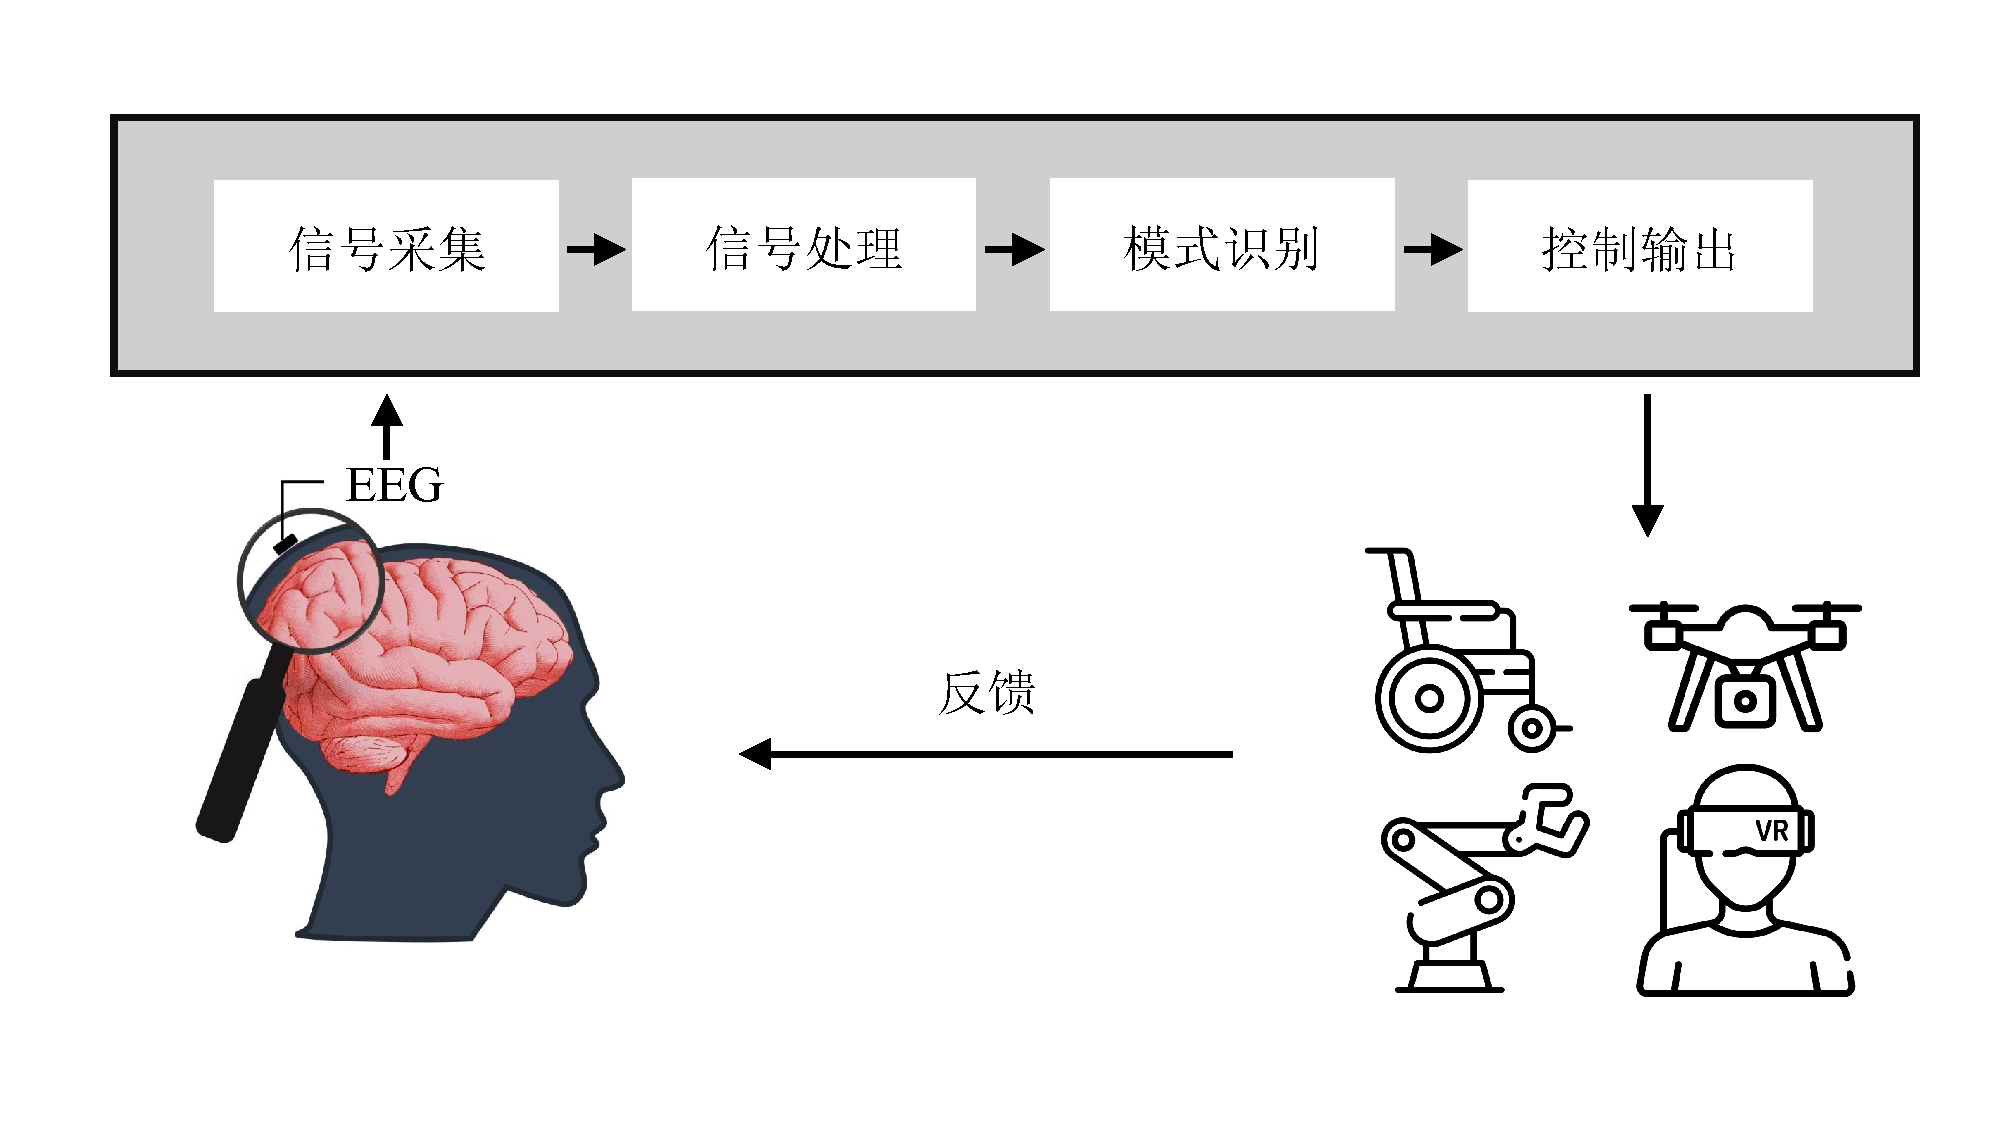
\includegraphics[width=0.5\textheight]{BCI系统构成.pdf}
	\caption{基于EEG的闭环BCI系统\cite{1-28}}
	\label{fig1-1}
\end{figure}

其通常包含四个主要组成部分:信号采集、信号处理、模式识别以及控制输出。当人脑受到特定的外界刺激,或者进行某类具体的思想活动时,其会产生对应类型的EEG信号。这些特定模式的EEG信号会被BCI系统精准获取,在进行适当的滤波降噪以及伪影筛除等预处理步骤后,被送往BCI系统的模式识别模块。模式识别算法通过对预处理后EEG信号进行特征提取,实现对当前人脑状态的预测或者辨识,解码人脑意图,并生成相应的控制指令,进行对外部设备的操控。外部设备的运行结果又会进一步反馈给使用者,从而形成控制闭环。

\subsection{EEG信号基本特征}
EEG作为一种成熟的脑科学研究手段,早在1875年便被英国内科医生Richard Canton首次发现。然而,由于采集设备的限制,直到1924年,
EEG才被德国科学家Hans Berger第一次系统记录下来\cite{1-20}。自此开始,EEG便被用来指代通过电极在人脑头皮表面收集到的生物电信号。这些由电极周围数量庞大的神经元电生理活动所组成的总体反应,包含了庞大的生理信息,是了解脑内连接和辨识大脑状态的有力工具。

由于EEG信号在时域上具有高度的非高斯性、非线性和非平稳性,因此从时域上难以直观地获取有价值的信息\cite{1-21,1-103}。然而,EEG具备十分显著的频域特征,这导致人脑的某些状态往往会与不同的EEG频段直接挂钩。在进行EEG分析时,频域特征是不可或缺的重要信息。一般情况下,人脑EEG信号的频率集中在0.2 Hz至60 Hz之间,并被分为五个主要频段:$\delta$、$\theta$、$\alpha$、$\beta$以及$\gamma$。各频段的常见脑区如图\ref{fig1-2}所示。这五个频段的主要特点如下:

\begin{figure}[!h]
	\centering
	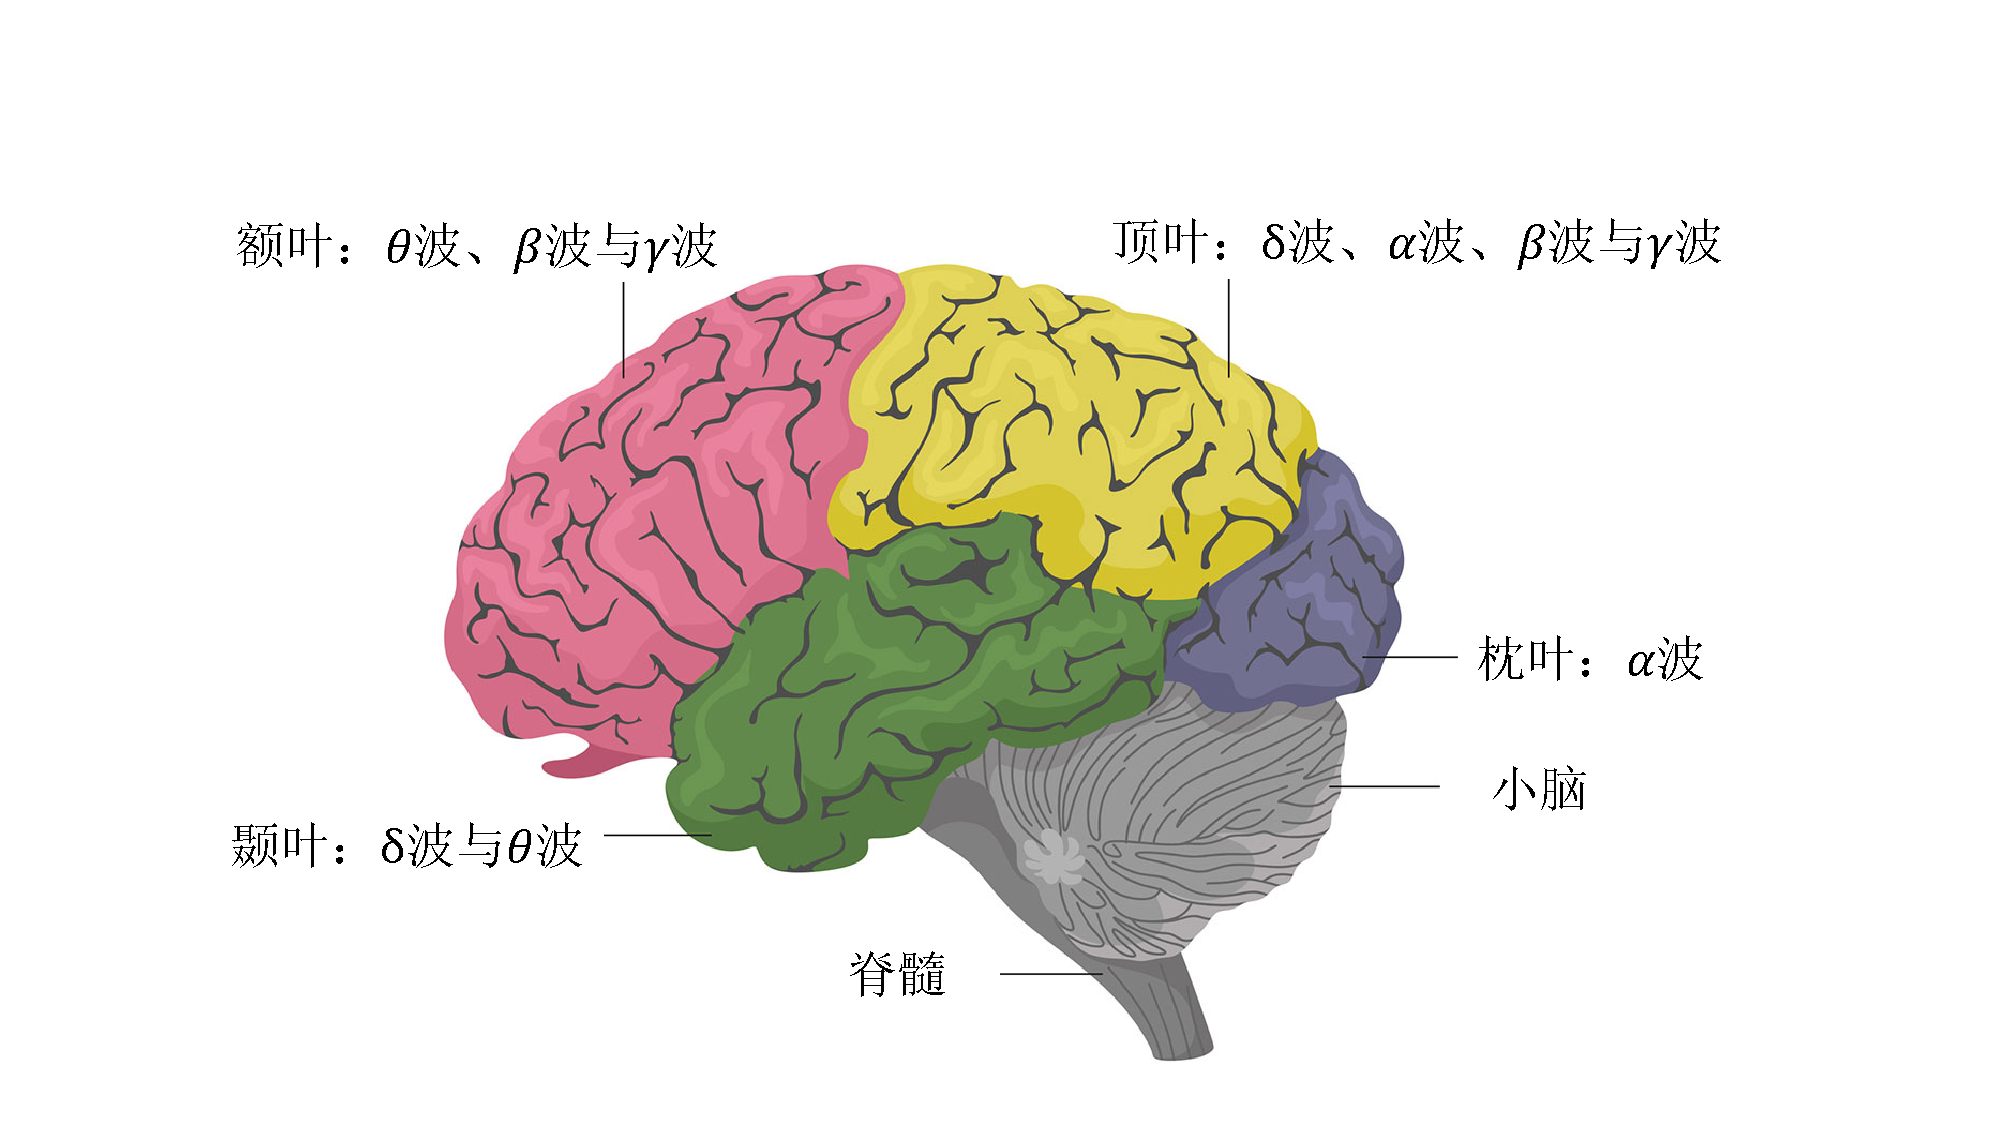
\includegraphics[width=0.45\textheight]{EEG脑区.pdf}
	\caption{不同频段EEG活跃脑区}
	\label{fig1-2}
\end{figure}

$\delta$频段:一般为0.2 Hz-4 Hz,幅值处于20 $\mu $V-150 $\mu $V之间。这一频段的信号通常出现于两类人群:(1) 处于沉睡状态或极度疲劳状态下的成年人颞叶区域,此时幅值相对较低;(2) 大脑尚未发育成熟的婴儿颞叶与部分顶叶区域,此时幅值相对较高。$\delta$频段代表了人体的无意识调节功能,平稳的$\delta$波有助于恢复疲劳,提升机体免疫能力。

$\theta$频段:一般为4 Hz-8 Hz,幅值处于100 $\mu $V-150 $\mu $V之间。$\theta$频段反映了人脑的潜在情绪与体验感受,当人发生情绪波动时会出现在大脑的颞叶和部分额叶区域。$\theta$波也与人脑的精神状态回复具有一定关联性,平稳的$\theta$波有助于提升创造性,放松心态。

$\alpha$频段:一般为8 Hz-13 Hz,幅值处于20 $\mu $V-100 $\mu $V之间。$\alpha$频段为人脑有意识活动与无意识活动的中间地带,是静息态EEG信号的主要成分。在人脑处于理想放松状态时,$\alpha$波将会出现在大脑的顶叶和枕叶区域。

$\beta$频段:一般为13 Hz-30 Hz,幅值处于5 $\mu $V-20 $\mu $V之间。$\beta$频段代表了人脑的有意识活动,在认知、推理、计算、阅读以及理解等任务中扮演着重要角色。$\beta$频段是人脑处于清醒状态下的主要频段,因此当其活动增强时,大脑会自动降低$\alpha$频段活跃程度。$\beta$波常见于大脑的额顶叶区域。

$\gamma$频段:一般为30 Hz-60 Hz,幅值活动范围较大。$\gamma$频段在人脑的学习与记忆环节常常发挥重要作用,高活跃度的$\gamma$波代表了个体具有较强的学习适应能力。当人脑处于记忆、学习以及冥想中时,$\gamma$波通常出现在额叶和额顶叶区域。

深入了解EEG基本特征,有助于BCI系统的合理搭建,并能够帮助BCI系统提升人脑状态辨识与控制意图解码的准确性。


\subsection{基于EEG的BCI系统范式}
为了将基于EEG的BCI系统应用于具体的现实环境,必须为实验的所有阶段选择特定的协议和范式。具体来说,使用者首先需要执行一个特定的任务(比如想象任务或者视觉任务),以学习如何调节他们的大脑活动,此时BCI会记录使用者的EEG信号。这些采集得到的信号将被作为训练数据,以生成该范式的神经解码器(模式识别算法)。之后,当使用者再次执行同类任务时,训练好的神经解码器便能成功进行BCI控制。

常见的EEG-BCI系统范式包括:稳态视觉诱发电位(Steady State Visual Evoked Potential,SSVEP)范式\cite{1-29,1-30}、事件相关电位(Event-Related Potentials,ERP)范式\cite{1-31,1-32}、运动想象(Motor Imagery,MI)范式\cite{1-33,1-34}和被动范式(Passive Paradigm)\cite{1-35}。
 
(1) 基于SSVEP范式的BCI系统

\begin{figure}[!h]
	\centering
	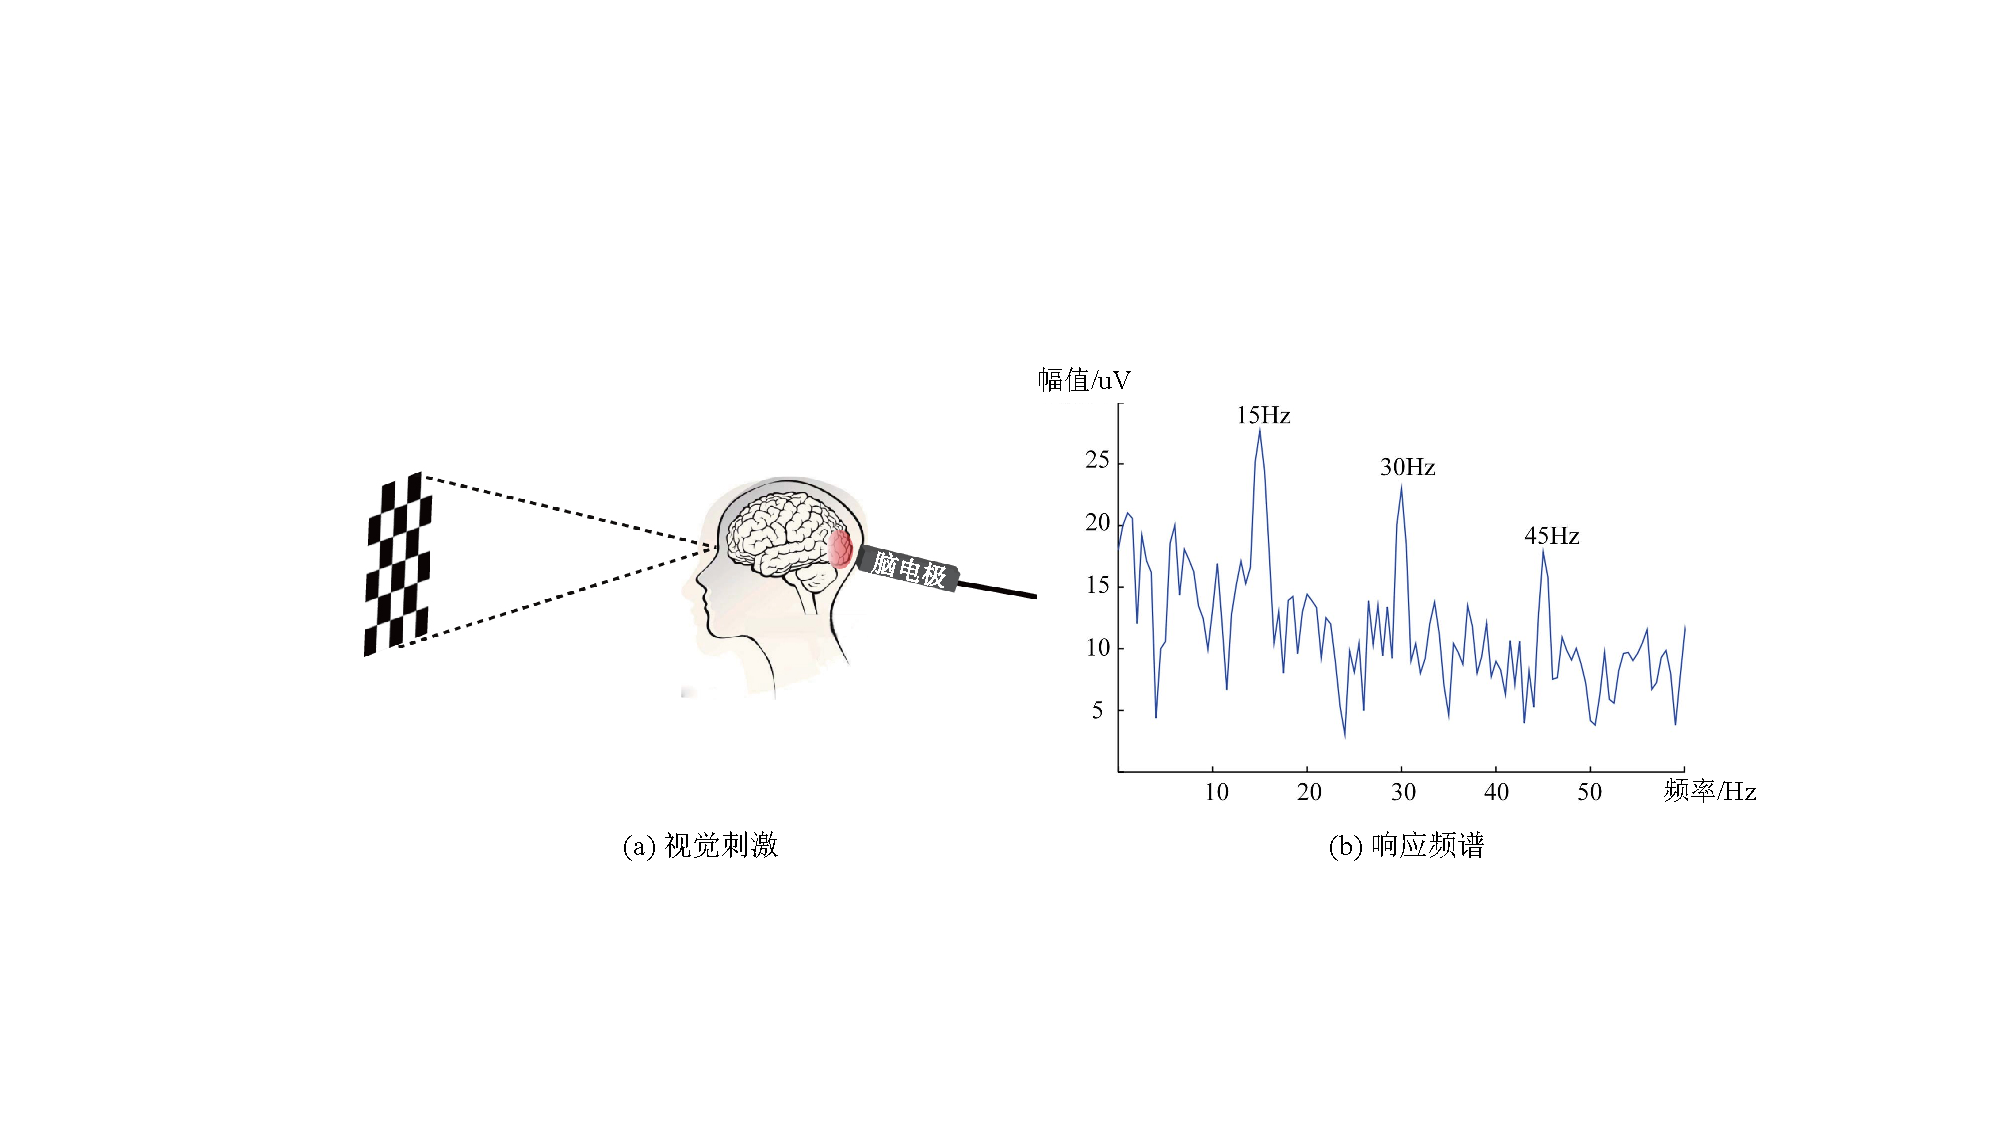
\includegraphics[width=0.61\textheight]{SSVEP.pdf}
	\caption{基于SSVEP范式的BCI系统}
	\label{fig1-3}
\end{figure}

SSVEP在诱发时,需要使用者将目光和注意力转移到闪烁的刺激源上,以唤起视觉皮层的电位响应,因此SSVEP范式又被称作光电驱动EEG(Photic Driving EEG)。在SSVEP范式中,投射到视网膜中央的恒定频率闪烁刺激会在人脑中产生与闪烁源频率相同的EEG信号。闪烁源的刺激频率可以在低频(1 Hz-3.5 Hz)到高频(75 Hz-100 Hz)范围内任意选择\cite{1-37}。闪烁刺激可以通过发光二极管或阴极射线管产生。在使用时,通过向使用者展示具有不同闪烁频率的多个闪烁目标,唤起使用者不同频段的EEG响应,之后通过EEG的频域特征来辨识使用者的观察意图。SSVEP范式的BCI系统实验内容如图\ref{fig1-3}所示。

SSVEP范式具有许多优点:首先,由于刺激来自于外界,这一范式无需进行训练便可应用于不同使用者。其次,闪烁刺激具有宽广的频段,可以生成大量不同指令控制多自由度的外部设备。最后,SSVEP的频率相较于ERP更便于区分,使基于这一范式的BCI系统具有更高的使用精度。然而,长时间的闪烁刺激也可能会导致受试者产生疲劳\cite{1-38}。并且由于在使用过程中需要注视刺激源,这种范式也不太适合有视觉障碍的使用者\cite{1-39, 1-40}。

(2) 基于ERP范式的BCI系统

ERP范式是指通过对特定事件类型的EEG信号进行平均,得到的事件关联响应特征。在ERP范式中,P300受到了最多的关注。P300本质上是ERP中的一个正峰,其大小在5 $\mu $V到10 $\mu $V之间,出现于对应事件发生的220 ms到500 ms后,如图\ref{fig1-4}。但是当事件间间隔小于250 ms-300 ms时,P300的定义会产生一定问题\cite{1-41},因为P300的响应将与后续事件出现重叠。

基于视觉的P300范式拥有极高的精度,可以在几分钟内实现系统校准,适用于大多数使用者。因此,使用者可以方便快捷地使用该系统对设备进行控制。但是,视觉P300需要长时间保持高度集中,这容易导致使用者出现疲劳问题\cite{1-32,1-42}。

\begin{figure}[h]
	\centering
	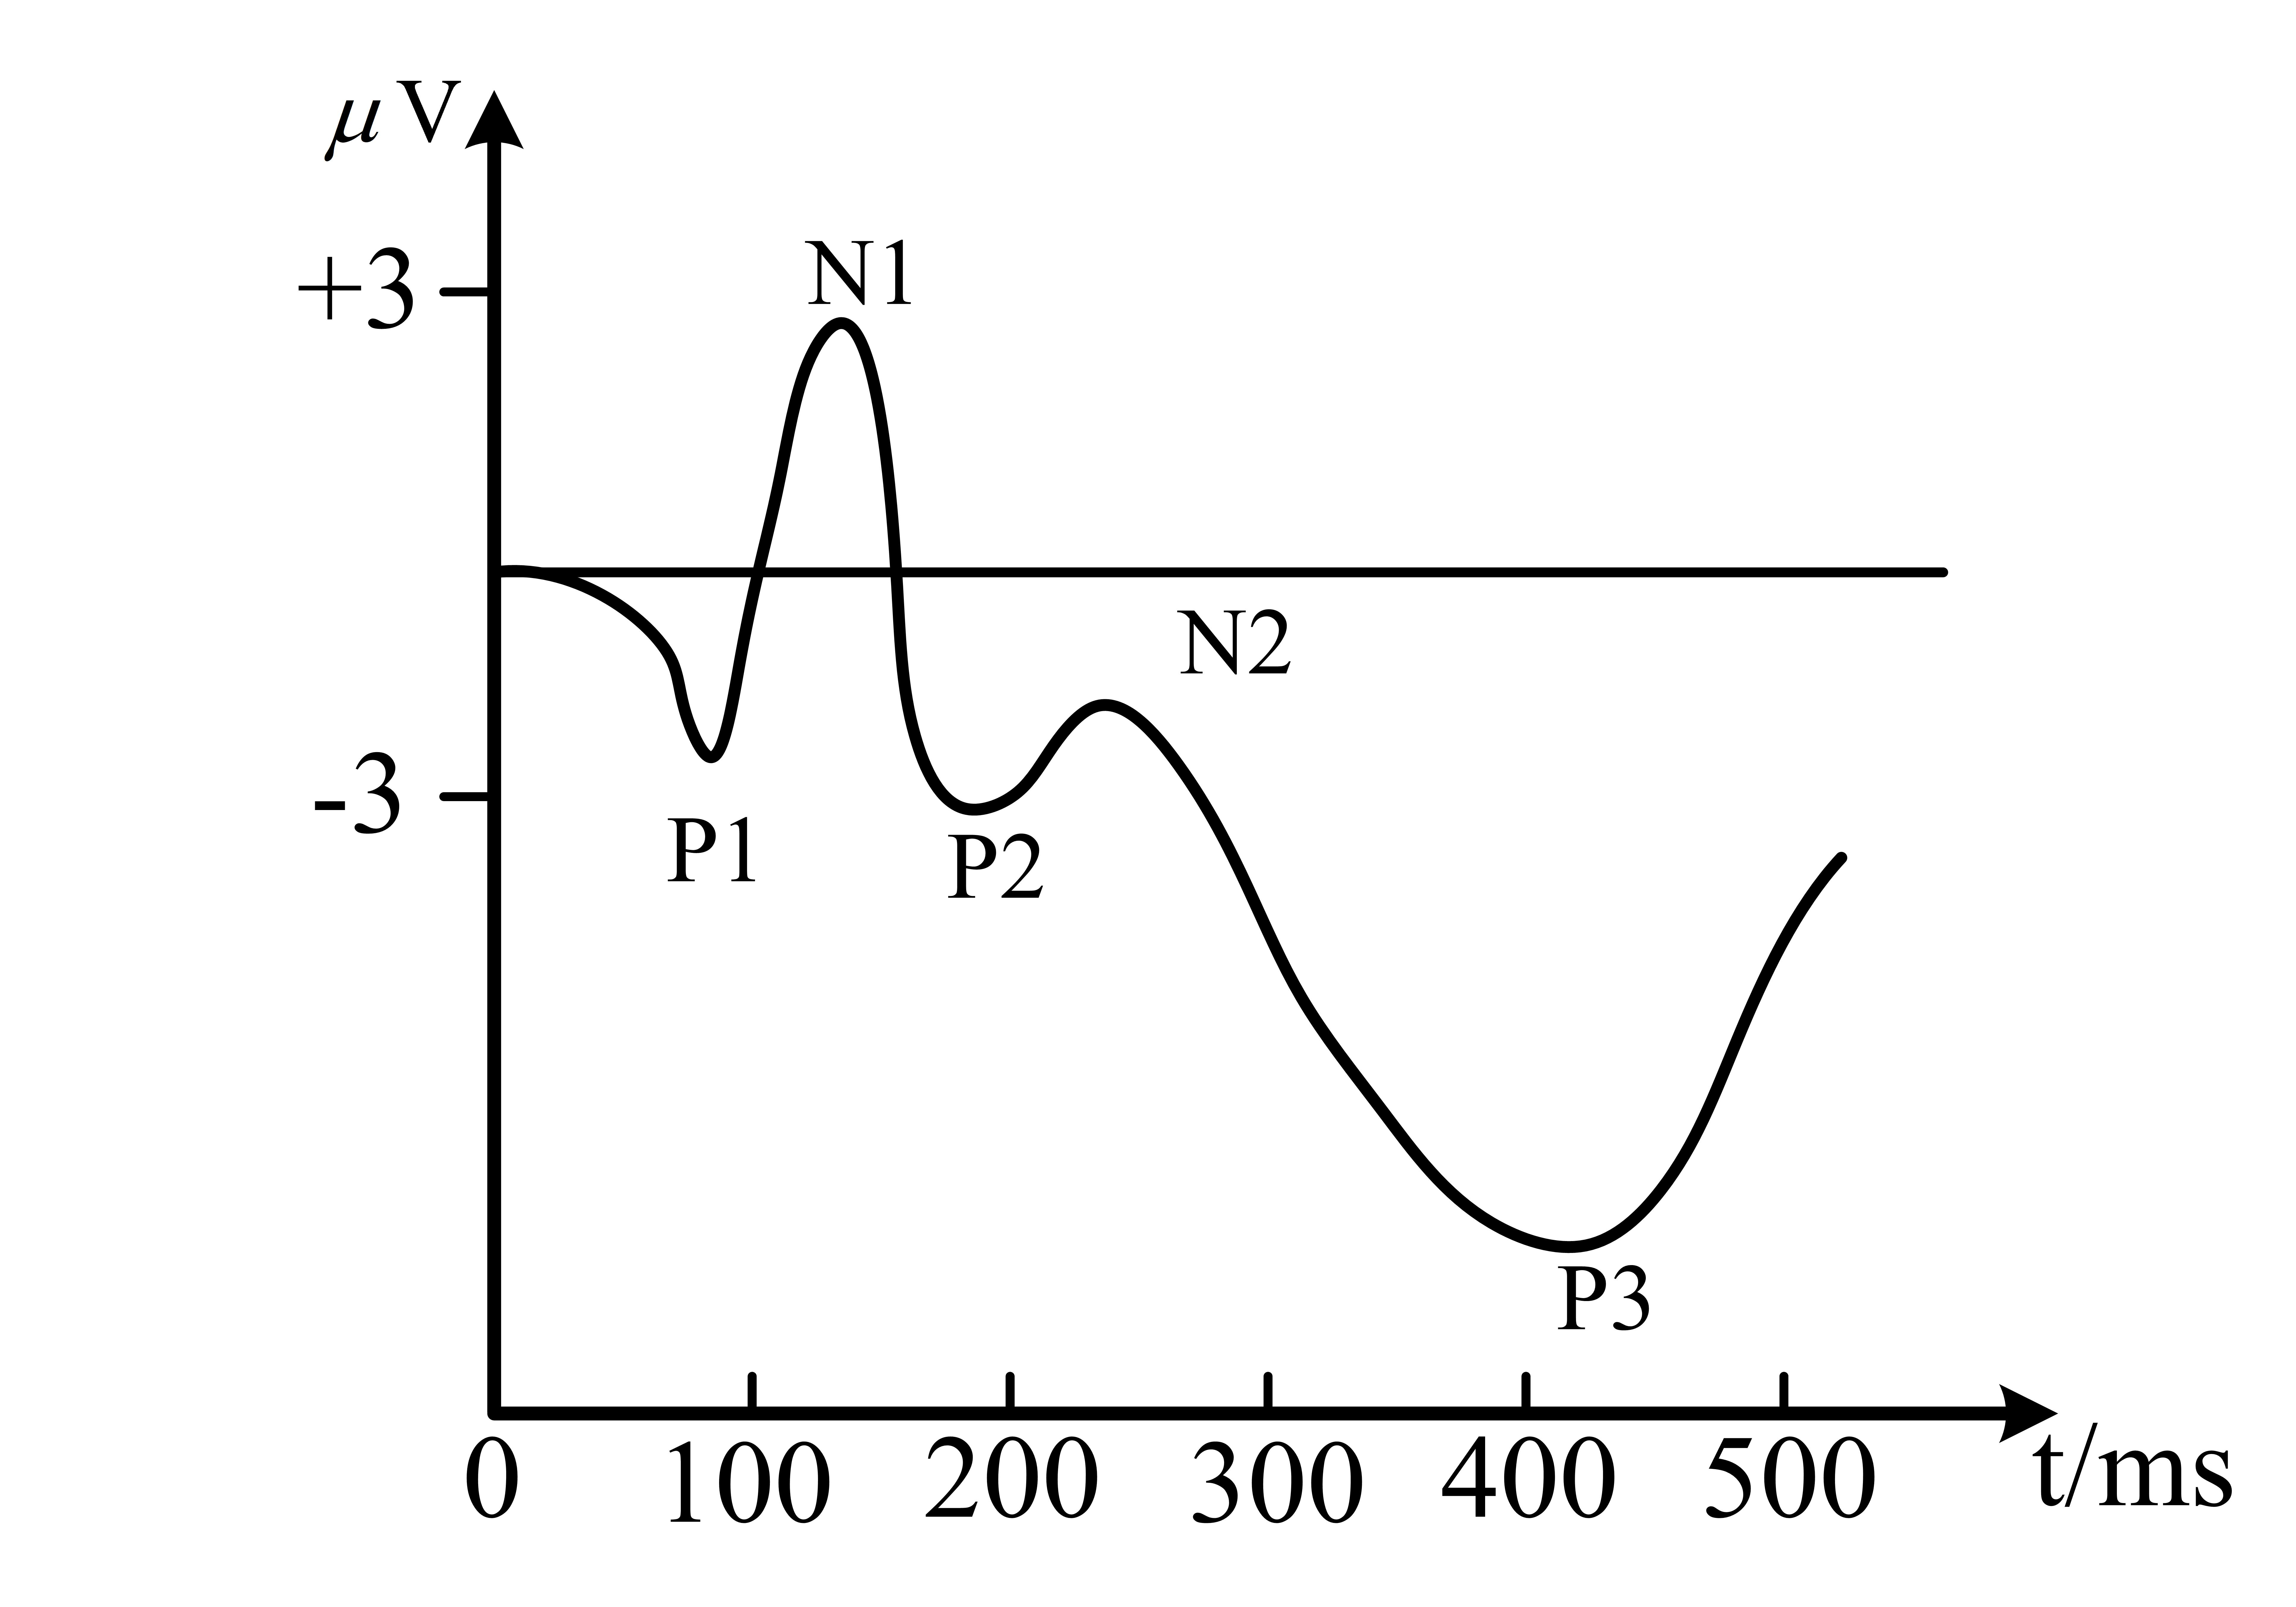
\includegraphics[width=0.3\textheight]{ERP.jpg}
	\caption{ERP相应特征}
	\label{fig1-4}
\end{figure}

(3) 基于MI范式的BCI系统

MI是人脑想象部分肢体的运动行为,而不真正执行相关动作的EEG范式。先前的研究已经证实,MI同样会激活大脑中负责产生实际动作的区域\cite{1-43}。MI在已有研究中被分类为感觉运动节律(SensoriMotor Rhythm,SMR)和想象身体运动(Imagined Body Kinematics,IBK)两类子范式。其中IBK需要使用者想象某一身体部位在三维空间的连续动作而被称为自然运动想象范式,但是这也对使用者的专业性提出了极高要求,并且需要配合较高性能EEG解码算法。因此,使用更为简单可靠的SMR范式是当前基于MI的BCI系统研究的重点。在SMR范式中,使用者需要想象身体进行一种具体运动(常见包括抬起脚、举起双手以及伸出舌头等),EEG解码算法通过分辨使用的运动意图,输出具体指令。

当进行动作想象时,人脑会在$\alpha$频段和$\beta$频段产生事件相关去同步现象(Event-Related Desynchronization,ERD)——对应频段的振幅降低;当动作想象结束后,相关频段振幅回升,即产生事件相关同步现象(Event-Related Synchronization,ERS)\cite{4-22,4-23}。特别的,在国际10/20系统的脑电极分布下,C3和C4电极位置获得的EEG信号中ERD和ERS现象尤为显著——这些电极位置位于感觉运动皮层的上方。MI中的ERD和ERS现象如图\ref{fig1-5}所示。

\begin{figure}[h]
	\centering
	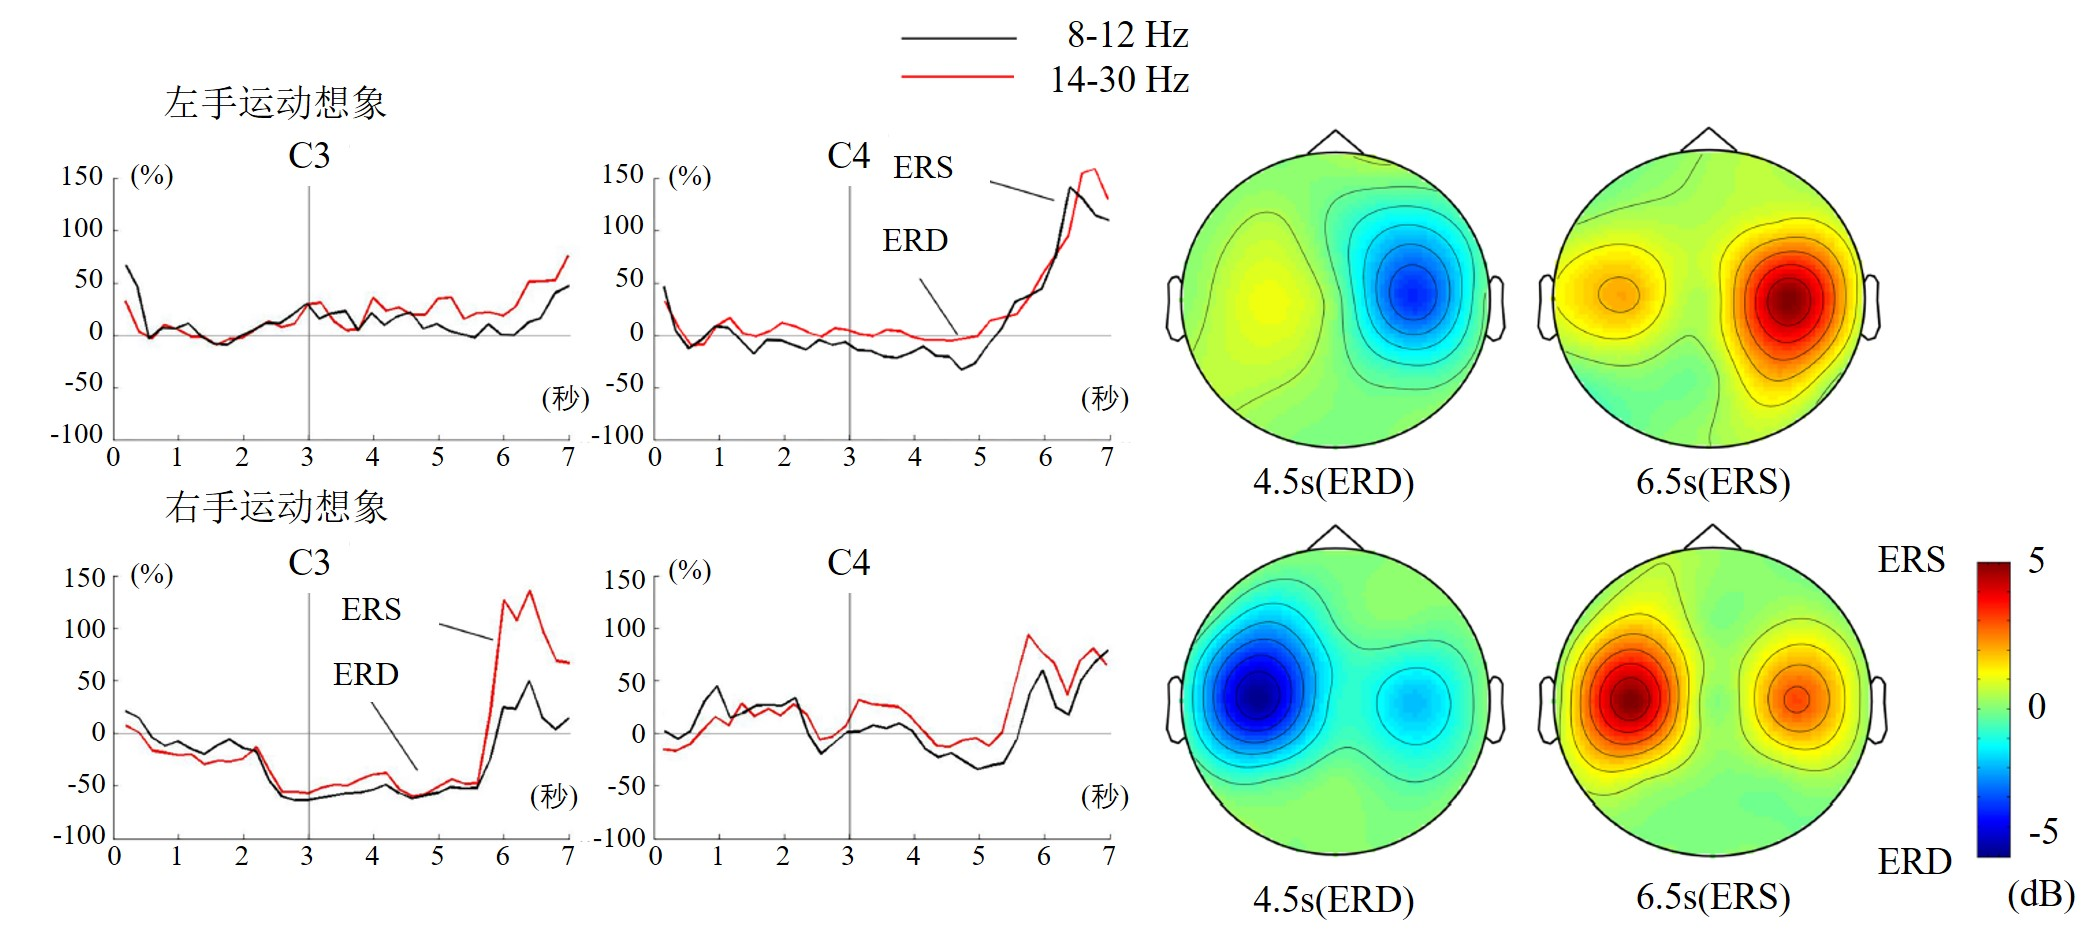
\includegraphics[width=0.60\textheight]{ERD-ERS.jpg}
	\caption{进行左右手MI任务时的ERD/ERS现象\cite{1-99}}
	\label{fig1-5}
\end{figure}

基于MI的BCI范式通过ERD和ERS现象能够进行较高精度的运动意图辨识,充分调动人体相关部位的运动神经。基于这一特点,MI在身体运动机能受损的康复治疗过程中具备极高的潜力,特别是在脑卒中患者康复领域\cite{1-44,1-45}。脑卒中患者由于脑部运动神经损伤而无法控制肢体正常运动,但是其大脑仍然保持了运动想象能力。同时,病人的患侧肢体运动机能仍然健全,因此可以通过重建神经映射通路重拾运动能力\cite{1-46,1-47}。近年来众多临床医学研究表明,基于MI的BCI系统在卒中后患者的康复进程中可以扮演重要角色\cite{1-48,1-102}。

(4) 基于被动范式的BCI系统

被动范式包括情景解释、情绪分类、意图辨识以及疲劳预警等无需进行外部刺激诱发的BCI范式\cite{1-36}。这类BCI范式不以控制意图解码为首要目的,而更关注于人脑当前状态辨识,目的是挖掘使用者的隐含信息来丰富人机交互进程。具体来说,精准的情绪辨识BCI可以让人机交互系统更加人性化,优化用户的使用体验。可靠的疲劳预警系统能够及时发现工作中的风险隐患,提醒相关人员停止作业,保证公民的生命财产安全。这一类型的BCI范式近年来同样得到了广泛关注\cite{3-28,3-29,3-30}。然而,与主动范式不同,被动范式的EEG信号往往不具有共通的显著时频域特征,这对EEG解码系统提出了较高的要求\cite{3-31}。如何设计具有一定泛化能力的被动范式BCI系统是当前亟需解决的难题。图\ref{fig1-6}展示了情绪分类EEG的采集过程。

\begin{figure}[h]
	\centering
	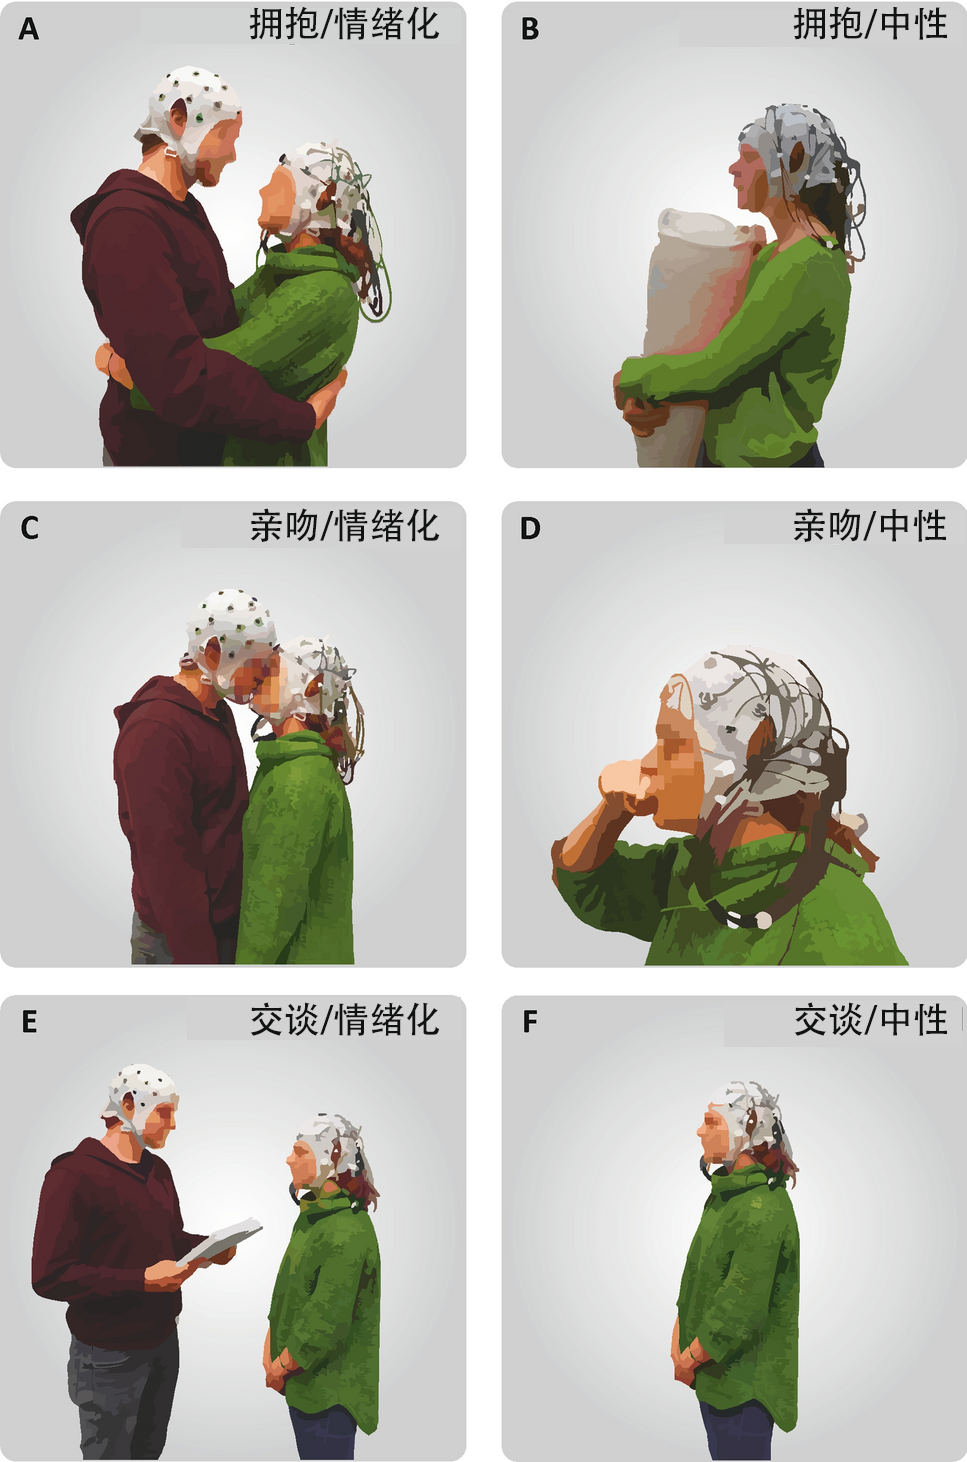
\includegraphics[width=0.3\textheight]{情绪辨识.PNG}
	\caption{情绪EEG采集\cite{1-49}}
	\label{fig1-6}
\end{figure}


不同范式的BCI系统所获取的EEG信号具有不同的分类难度,其中SSVEP和ERP范式由于其显著的时频域特点而相对容易辨识。MI范式和被动范式的EEG信号则由于其难以寻找通用性特征仍面临着分类精度不足的问题,设计合理的分类辨识模型是BCI走向实际应用的关键。


\subsection{国内外EEG采集设备}
EEG采集设备在发展过程中,逐渐分化出了侵入式\cite{1-50}与非侵入式\cite{1-51}两条不同的分支。

侵入式EEG采集设备追求可靠的信号质量,更高的信噪比以及更少的外部生理信号干扰,直接将EEG电极通过手术的方式植入使用者大脑内部。这一采集手段的EEG电极直接与大脑进行接触,使其在拥有较为纯净优质信号的同时,也为使用者带来巨大的手术风险,直接对使用者的日常生理活动造成负面影响。因此,基于侵入式的EEG 采集设备在医疗科研领域拥有广阔前景\cite{1-52},但其并没有在现实生产生活中得到推广\cite{1-53}。图\ref{fig1-7}展示了侵入式脑电极在大脑中的排布方式。

\begin{figure}[h]
	\centering
	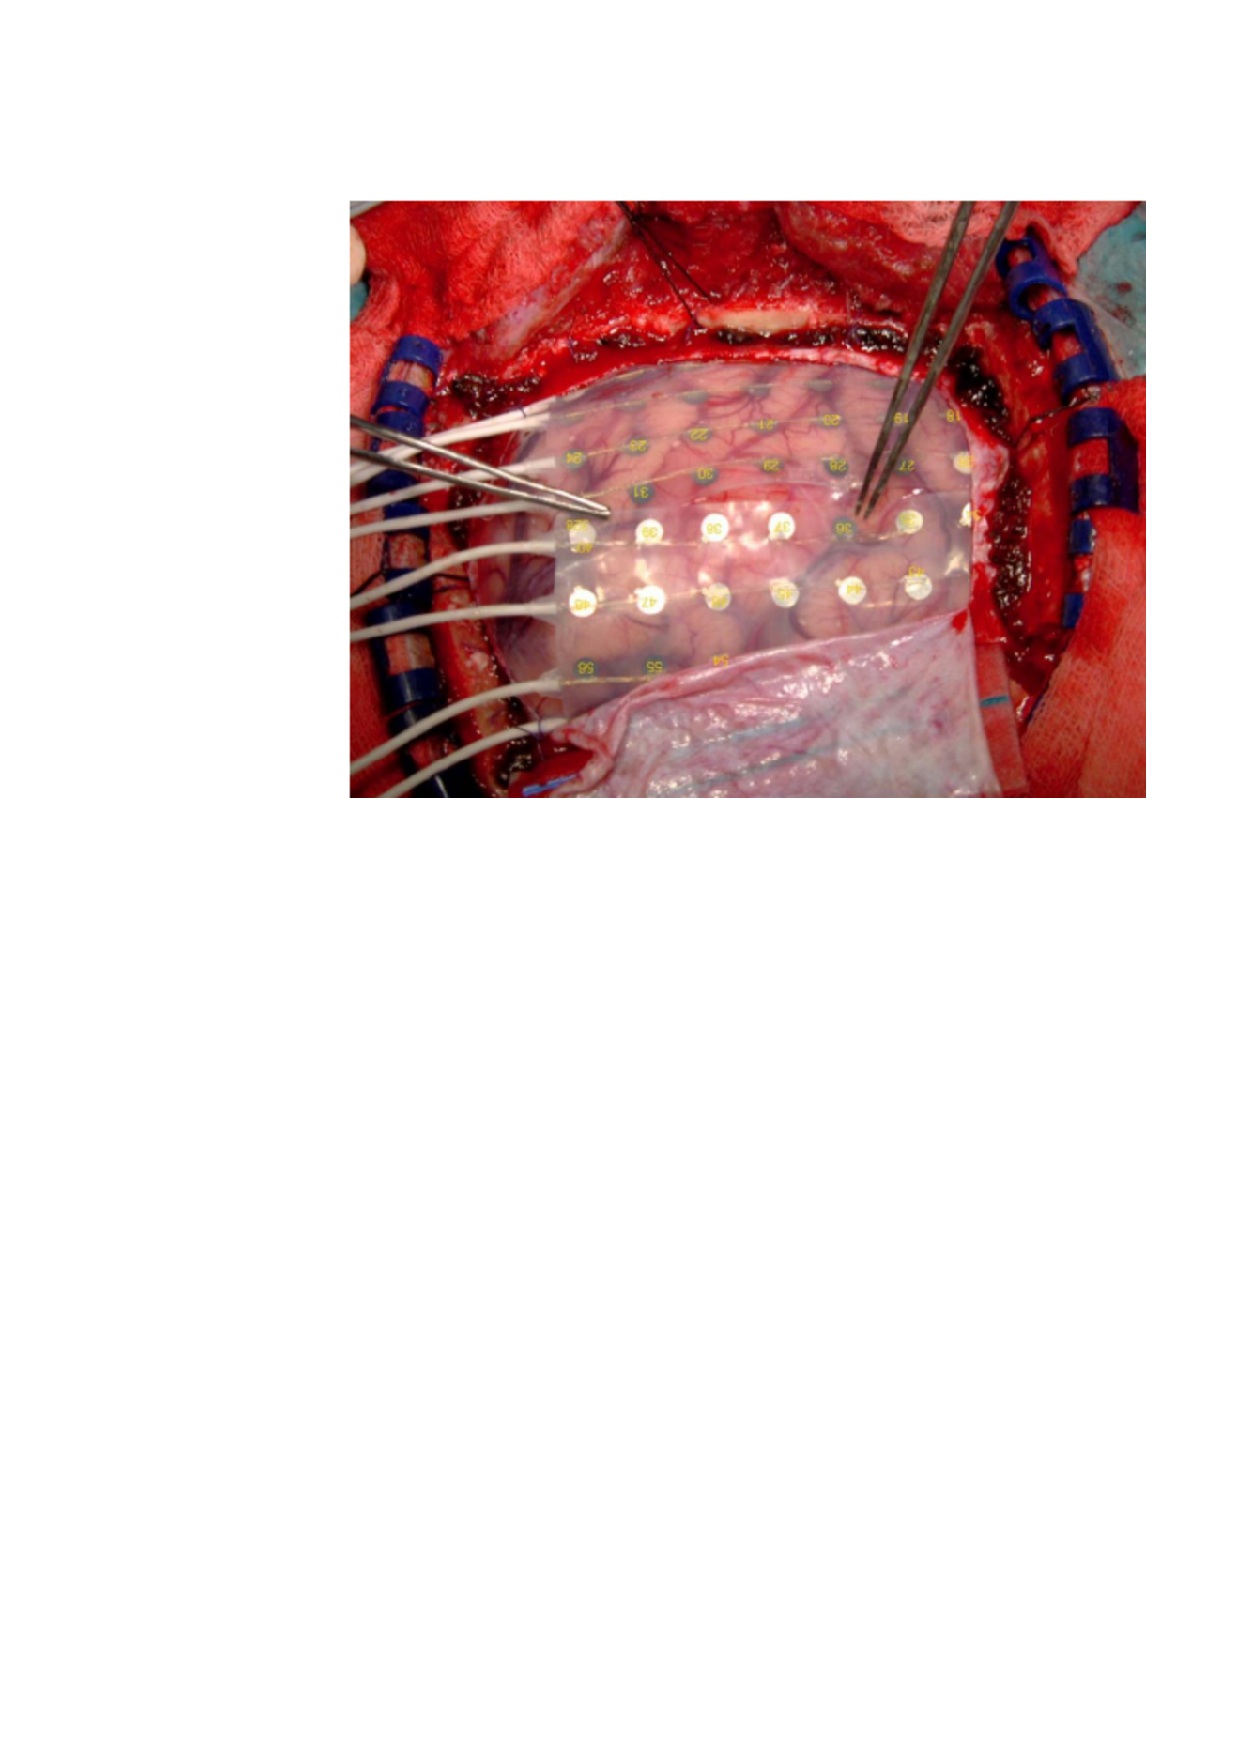
\includegraphics[width=0.33\textheight]{侵入式.pdf}
	\caption{侵入式EEG电极排布\cite{1-54}}
	\label{fig1-7}
\end{figure}


非侵入式EEG采集设备通过安置在大脑皮层外侧的脑电极进行获取,这些电极通常嵌入在脑电极帽中。这种采集手段的目的在于追求实用性,因为其无需进行手术,电极安装过程较为简便,没有过高的使用门槛,成本远低于侵入式设备。非侵入式EEG采集设备保留了高时间与空间分辨率的优点,并且其信号信噪比仍处于可接受的范围,因此在近年来得到了广泛关注\cite{1-55}。本文的工作即基于非侵入式EEG采集设备展开。

\begin{figure}[h]
	\centering
	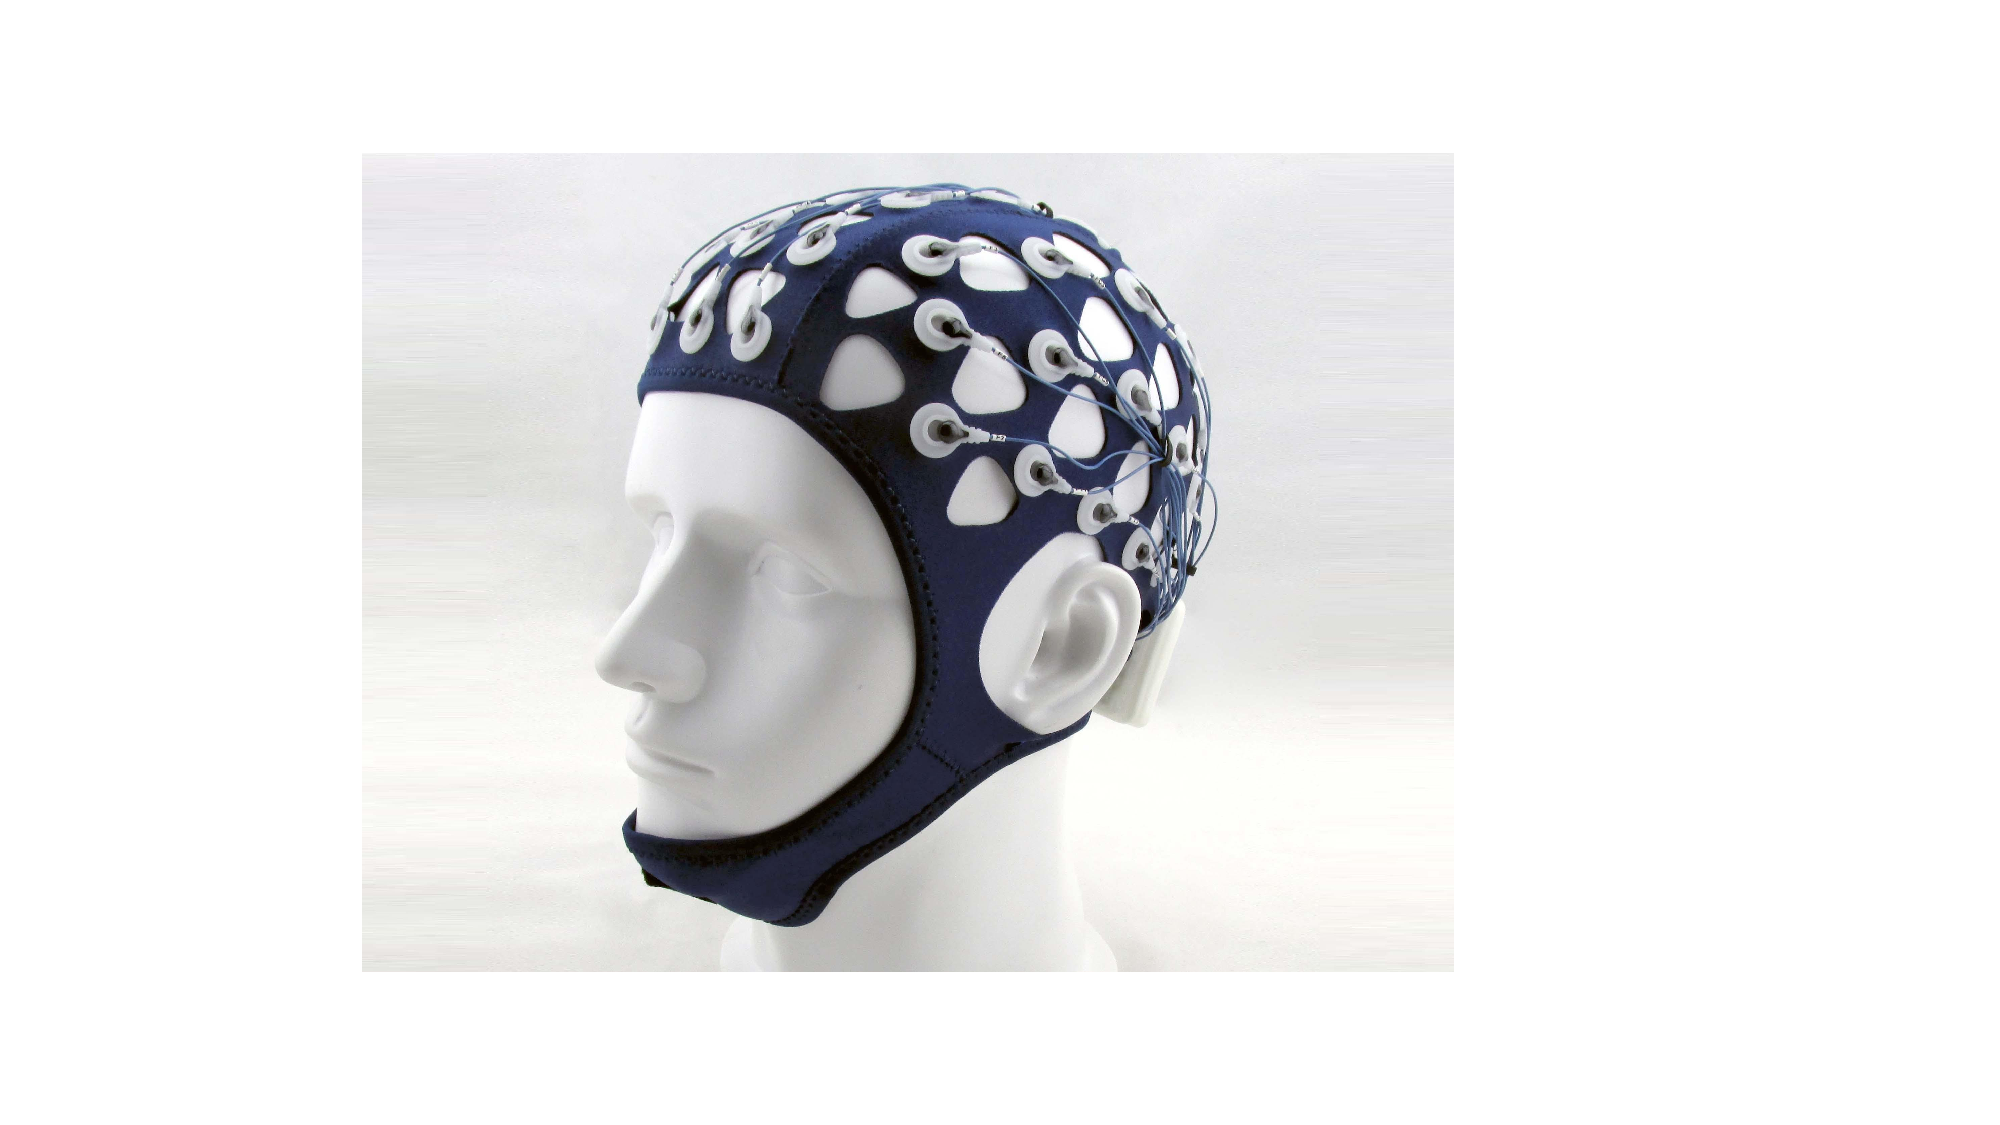
\includegraphics[width=0.33\textheight]{非侵入式.pdf}
	\caption{非侵入式EEG电极排布}
	\label{fig:graph3}
\end{figure}

当前国内外EEG采集设备已经具备了一定的成熟度,其中国外EEG研究起步较早,因此发展速度较快,产品种类较多。具有代表性的包括Neuroscan公司的Neuroscan Amplifiers系列产品、EGI公司的GTEN-200系列产品、Emotiv公司的便携式人机交互系统等。Neuroscan Amplifiers系列作为研发最早的EEG采集设备之一,已经发展出了十余种性能优异的不同采集子系统。其产品覆盖面较广,拥有29通道、32通道、64通道以及256通道等多种应对不同需求的EEG采集设备。其中常见的SynAmps RT 64-channel Amplifier设备能够以20000 Hz同时采集64通道EEG信号,每个通道包括一个24位的A/D转换器。这个采集系统除了用于EEG采集的导联盒和脑电极帽以外,还包括专用的电源盒(Power Unit)和控制盒(System Unit)。SynAmps RT 64-channel Amplifier系统的整体重量在10 kg以上,售价超过10万元,且体积较为庞大。EGI公司的GTEN-200系列产品能够采集32-256通道的EEG数据,其配套有先进的成像软件,能够绘制逼真的高分辨率人脑模型,是当今最先进的非侵入性神经调节系统之一。GTEN-200系列的64通道产品整体售价超过50万元,并且系统较为庞大,操作流程复杂。与前两种主要面向医疗科研领域的产品不同,Emotiv公司的便携式人机交互系统面向普通人的日常生活场景。其使用16通道的干电极采集EEG信号,并通过蓝牙对外设进行控制。它的设计理念更倾向于便携与日常使用,因此采集信号的质量较差。国内neuracle公司的EEG采集设备也已经得到了相关领域的认可,其设计生产的系列产品同样具备优异的采集性能与人脑状态辨识能力。

通过上述介绍可以看到,高精度的多通道EEG采集设备往往体积庞大,操作环节复杂,价格极高,仅能面向医疗科研使用。消费级的EEG采集设备存在着通道数较少,信号质量不佳的问题。因此,设计开发一款体积较小,通道数量较多,价格亲民的EEG采集设备对BCI系统的落地与推广具有一定的现实意义。本文将遵循这一思路,设计基于EEG的BCI系统,并对采集得到的EEG信号进行辨识分析。

\section{基于深度学习技术的脑电信号分析}
为了真正意义上实现BCI系统的广泛应用,BCI系统所收集的EEG信号能否被准确辨识已成为当前BCI性能评估的一个重要指标。针对不同的EEG范式,相关研究人员提出了众多特征提取方法,比如傅里叶变换(Fourier Transform)、表面-拉普拉斯变换(Surface-Laplacian Transform)、共空间模式(Common Spatial Patterns,CSP)以及基于熵的分析方法\cite{1-56, 1-57, 1-58, 3-11}。这些特征与支持向量机(Support Vector Machine,SVM)、近邻分类器(Nearest Neighbor Classifiers)以及逻辑回归(Logistic Regression)等传统机器学习分类器的结合为BCI系统的实现做出了巨大贡献\cite{1-59,1-60,1-61}。然而,基于这一设计思路的模型较为依赖于设计者的专业知识,缺乏足够的泛化性能。提升模型泛化性能的直观方法是增加通用信息的权重,并通过精确选择与任务相关的EEG通道来提高分类性能\cite{1-62}。此外,直接寻找关键性特征将为BCI系统带来更多的性能收益\cite{1-63}。

深度学习技术在过去十年中发展迅速,在图像处理和复杂时间序列分析中表现出强大的分类和辨识能力\cite{1-64}。经典的深度学习模型包括多层感知机(MultiLayer Perceptron, MLP)\cite{1-68}、循环神经网络(Recurrent Neural Networks, RNN)\cite{1-69}、玻尔兹曼机(Deep Boltzmann Machines, DBM)\cite{1-70}和卷积神经网络(Convolutional Neural Networks, CNN)\cite{3-21}等,其典型结构如图\ref{fig1-8}所示:

\begin{figure}[!h]
	\centering
	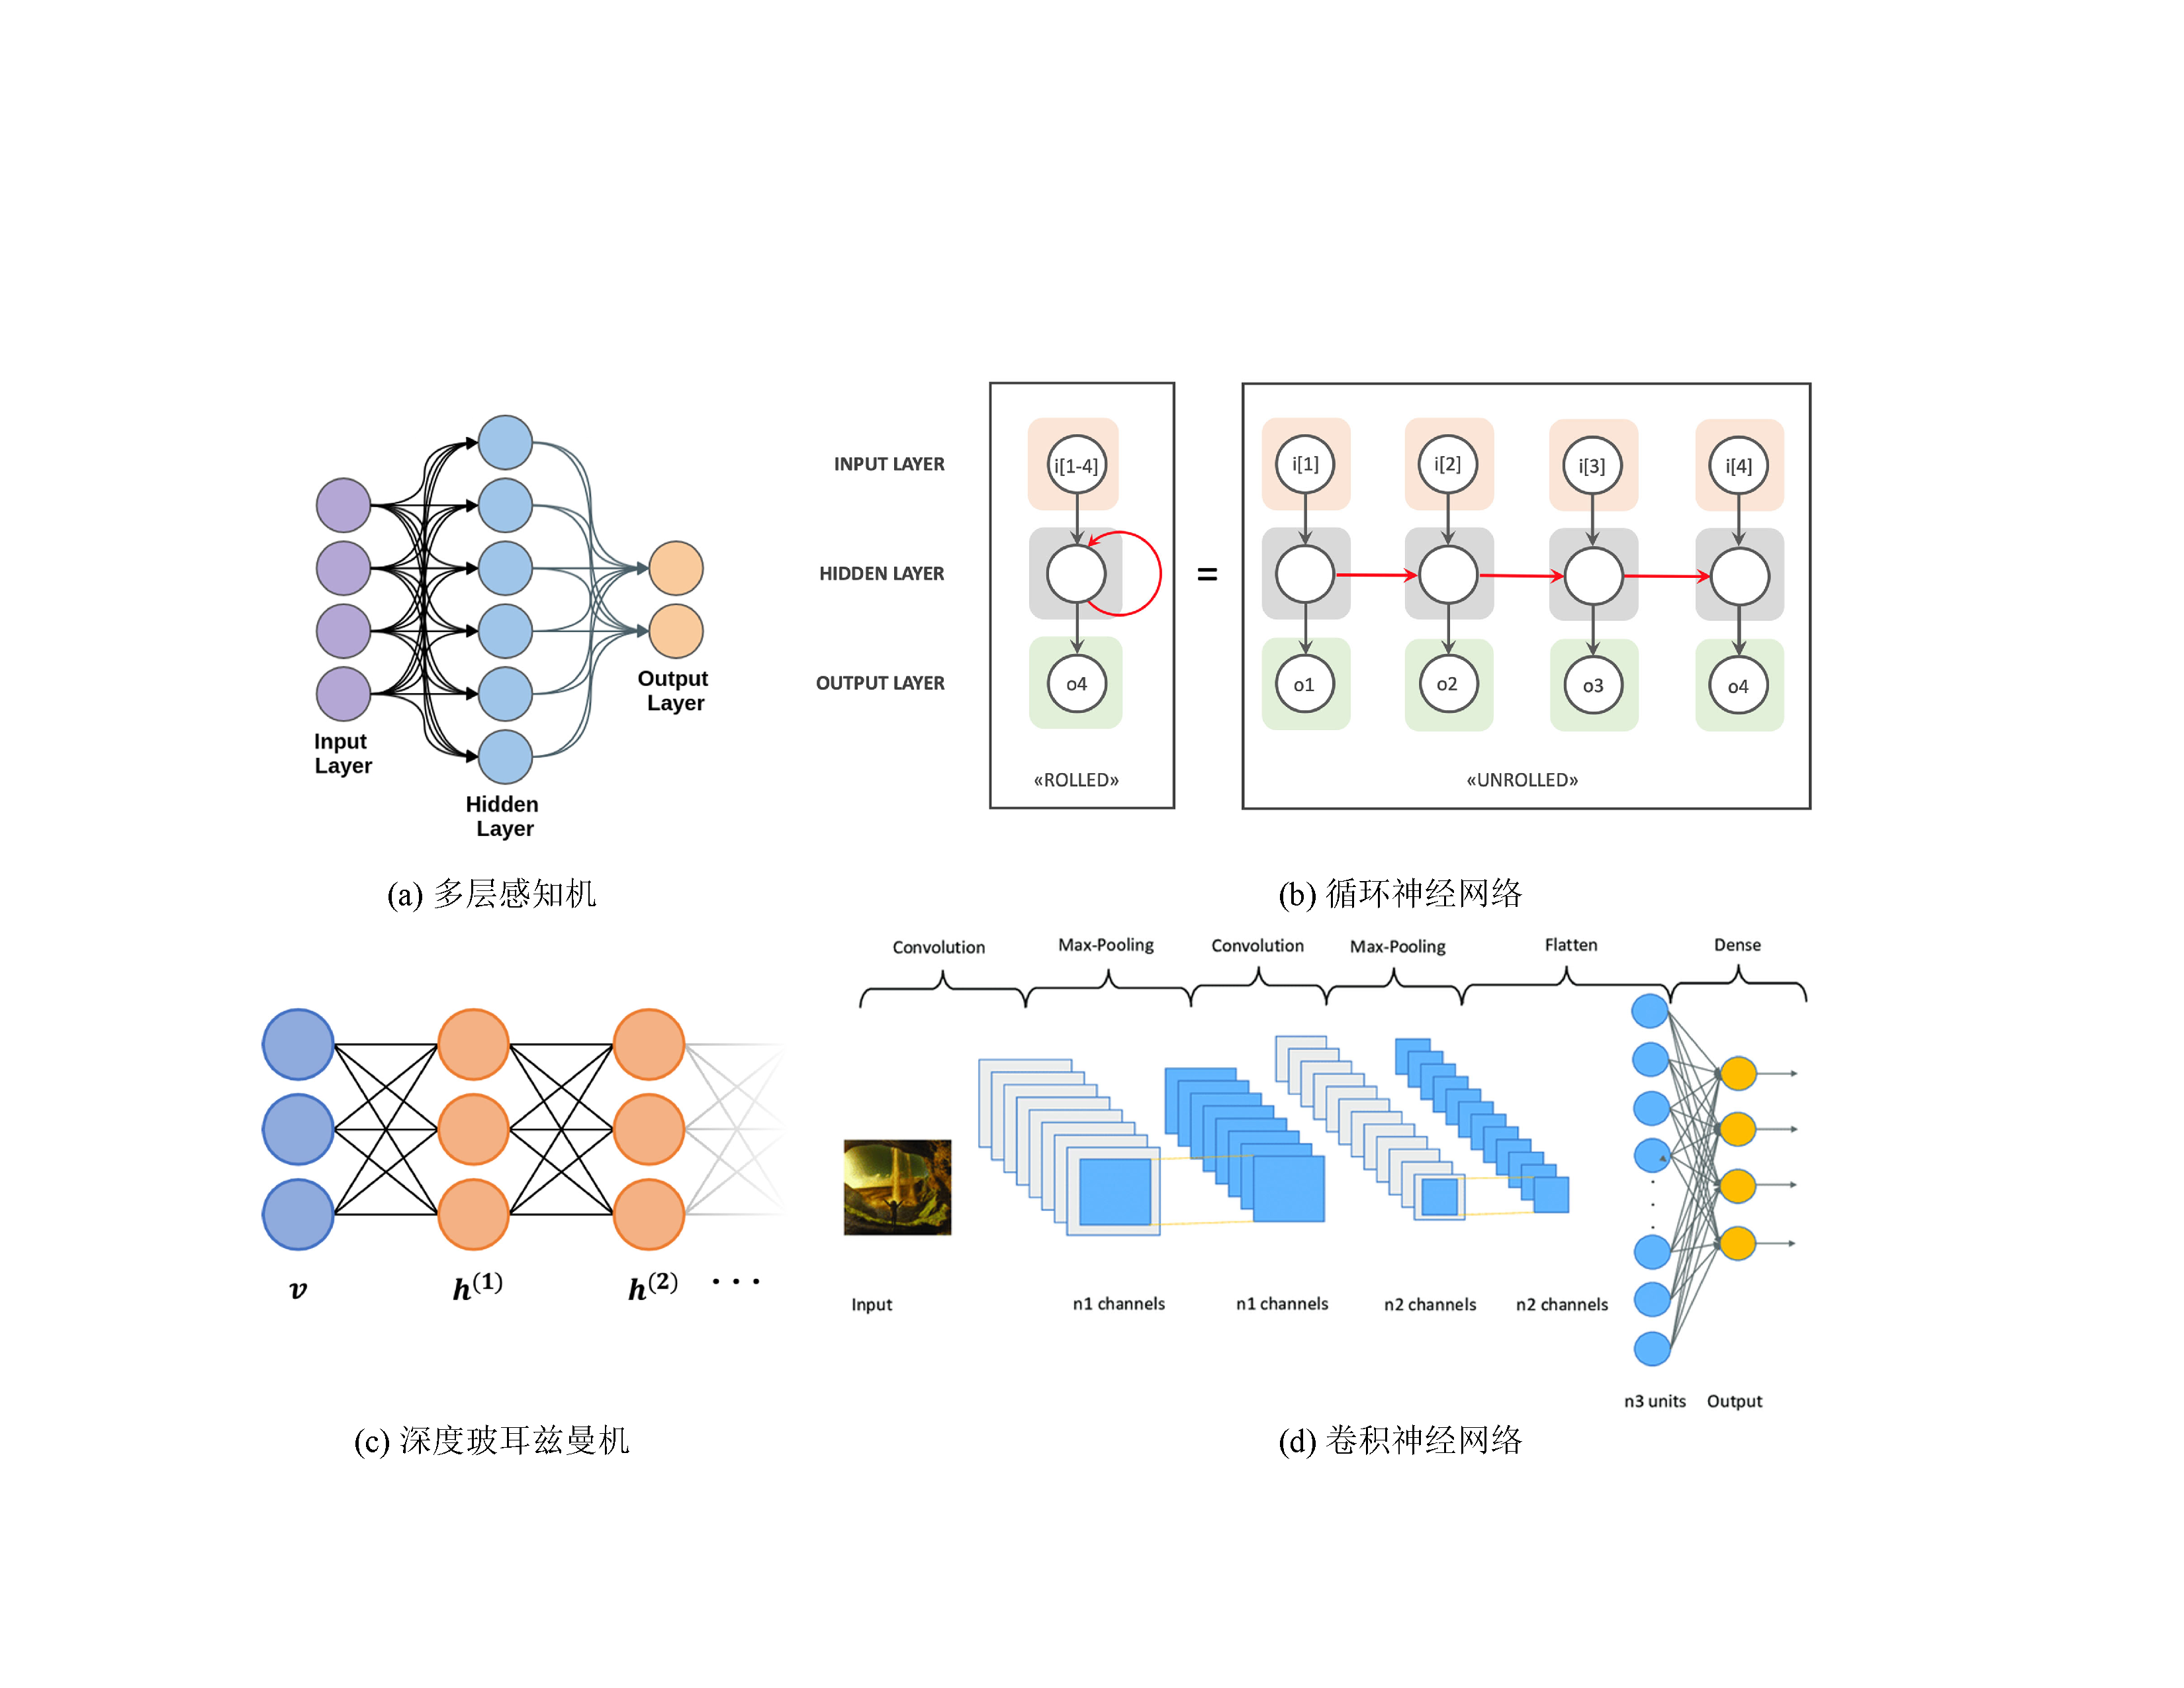
\includegraphics[width=0.60\textheight]{DL.pdf}
	\caption{深度学习模型典型结构}
	\label{fig1-8}
\end{figure}

深度学习模型具备的数据驱动和强大的特征提取能力,使其能够从大量的EEG信号中挖掘通用特征,减轻模型设计对于专家知识的依赖性。无论是基于主动范式SSVEP,ERP以及MI的EEG信号,抑或是基于被动范式情绪,疲劳以及脑负荷的EEG信号,深度学习均在其上取得了极具竞争力的结果\cite{1-66,1-67}。Gao等人\cite{1-65}基于EEG信号的时空特性,针对性的改造了卷积神经网络,引入具有时间和空间属性的卷积模块,在基于EEG的疲劳辨识任务中取得了极高的准确率。Xu等人\cite{1-71}在循环生成对抗网络(Cycle-consistent Adversarial Networks,CycleGAN)的基础上,保留EEG信号的频域特征与空间信息,生成脑卒中患者的EEG数据以扩展训练数据样本数量,实现对卒中患者运动意图的有效辨识。Ma等人\cite{1-72}成功地融合了深度置信网络(Deep Belief Network,DBN)和压缩感知技术,有效降低了DBN的训练复杂度,并将其成功应用于EEG分类。Tsiouris等人\cite{1-73}利用预训练策略,寻找LSTM模型种各模块的最优结构,之后构建两层LSTM网络对基于EEG的癫痫发病情况进行预测,为癫痫疾病的治疗提供辅助。He等人\cite{1-74}基于图注意力网络(Graph Attention Networks)和双向LSTM挖掘癫痫EEG数据的时域特征,并根据当前时刻的前后状态做出最终决策。结果表明,这一模型能够在两种常见的公开数据集上取得当下最优的结果。Khademi等人\cite{1-75}设计了一种混合结构的端到端MI范式EEG信号分类模型。其同时搭建三种不同的模型结构以应对单一模型可能出现的梯度消失或者表征能力不足问题,并使用迁移学习和数据增强算法提升模型的泛化性能。最终的结果表明,其拥有当下最具竞争力的MI辨识性能。

\section{神经架构搜索技术的发展及其与脑电信号辨识研究的融合}
尽管基于深度学习的EEG研究已经取得了瞩目的成果,但是这些方法也继承了深度学习模型结构设计困难、需要专业的设计经验与先验知识、依赖长时间的人工调试和优化等问题,阻碍了BCI系统的实现和普及。针对上述问题,神经结构搜索(Neural Architecture Search,NAS)概念应运而生\cite{1-76}。遗传算法\cite{1-77}、强化学习\cite{3-33}和贝叶斯优化算法\cite{1-78}已被成功应用于NAS进程中,这些方法在一定程度上解决了网络架构设计的问题,使模型根据数据信息自动获取合适的网络架构成为可能。

基于某种搜索策略,依靠预定义的候选操作集和搜索空间来探寻不同网络架构带来的性能变化,是NAS算法的设计策略。通过对生成的子网络的性能进行排序,并反馈不同架构带来的性能变化,搜索策略被不断优化。当得到的子网络满足网络性能要求时,搜索过程就会停止,并得到当前条件下的最佳网络架构\cite{1-76}。举例来说,基于神经网络的内部结构可以被编码为可变长度字符串的特性,利用强化学习能够生成最佳网络架构\cite{1-79}。Baker等人\cite{1-80}提出了“Meta-QNN”,它创新性地将网络架构搜索建模为马尔可夫决策过程,并使用强化学习中的Q-learning算法来寻找最佳CNN架构。为了提高计算速度,Zoph等人\cite{1-81}提出了“NASNet ”搜索模型,即先在一个小数据集上搜索网络结构,然后再迁移到一个大数据集上,从而减少结构搜索过程中的资源消耗,这一搜索策略被命名为代理搜索。Bender等人\cite{1-88}在已用NAS算法的基础上,创新性地将CNN架构设计为多个“Cell”结构的堆叠,而“Cell”结构被看作是一个包含N个有序节点的有向无环图。这一名为“one-shot”的结构设计,成为了后续NAS算法的基础。图\ref{fig1-9}展示了经典的“one-shot”搜索框架。

\begin{figure}[!h]
	\centering
	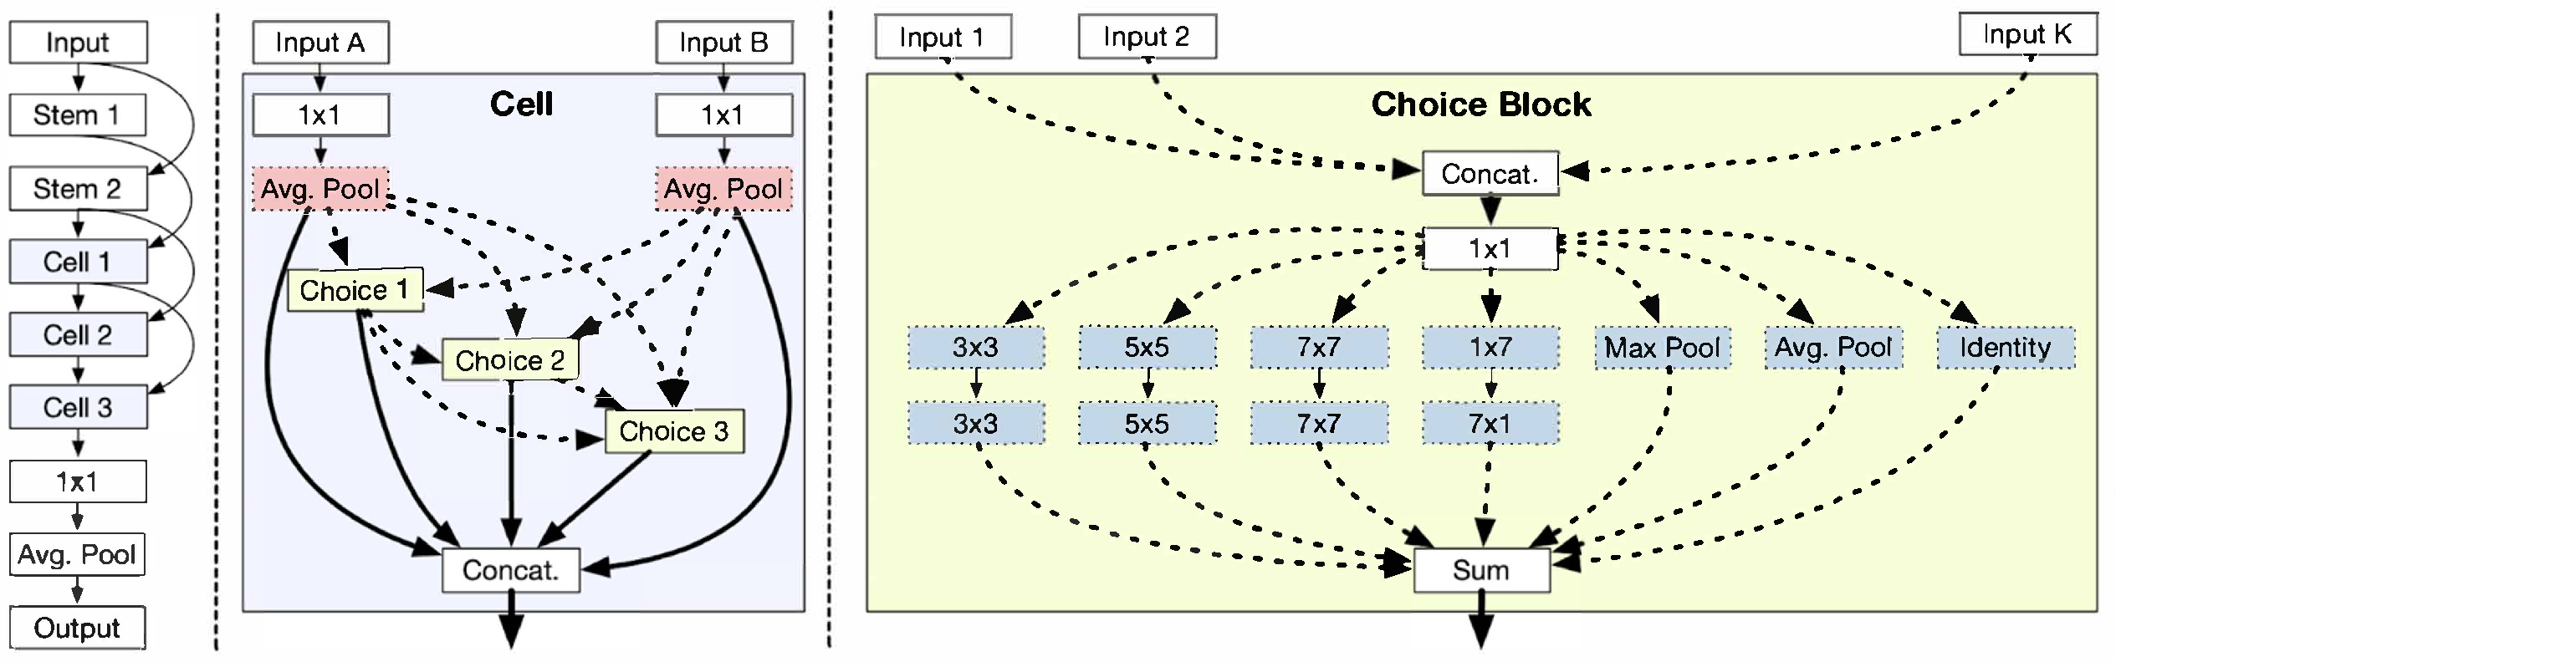
\includegraphics[width=0.60\textheight]{NAS.pdf}
	\caption{“one-shot”搜索框架\cite{1-88}}
	\label{fig1-9}
\end{figure}

然而,上述方法并没有改变NAS过程作为一个“黑箱”的本质,为了解决这个问题,基于梯度的NAS算法被开发出来。DARTS\cite{3-34}算法遵循Bender等人\cite{1-88}的设计,在“one-shot”搜索框架的基础上将梯度引入模型结构搜索中。基于梯度的算法同时优化了模型的结构权重和层权重,有效减少了结构搜索的时间和性能消耗。为了进一步减少内存占用,在DARTS的基础上,P-DARTS\cite{1-82}和PC-DARTS\cite{3-7}被研发出来,并取得了巨大的成功。PC-DARTS的成功不仅取决于其创新的部分通道搜索算法,而且还取决于其继承的DARTS搜索空间。DARTS的模块化搜索结构,连续的搜索空间合理降维了庞大的搜索区域,进一步提升了搜索效率。图\ref{fig1-10}展示了PC-DARTS的搜索流程。

\begin{figure}[!h]
	\centering
	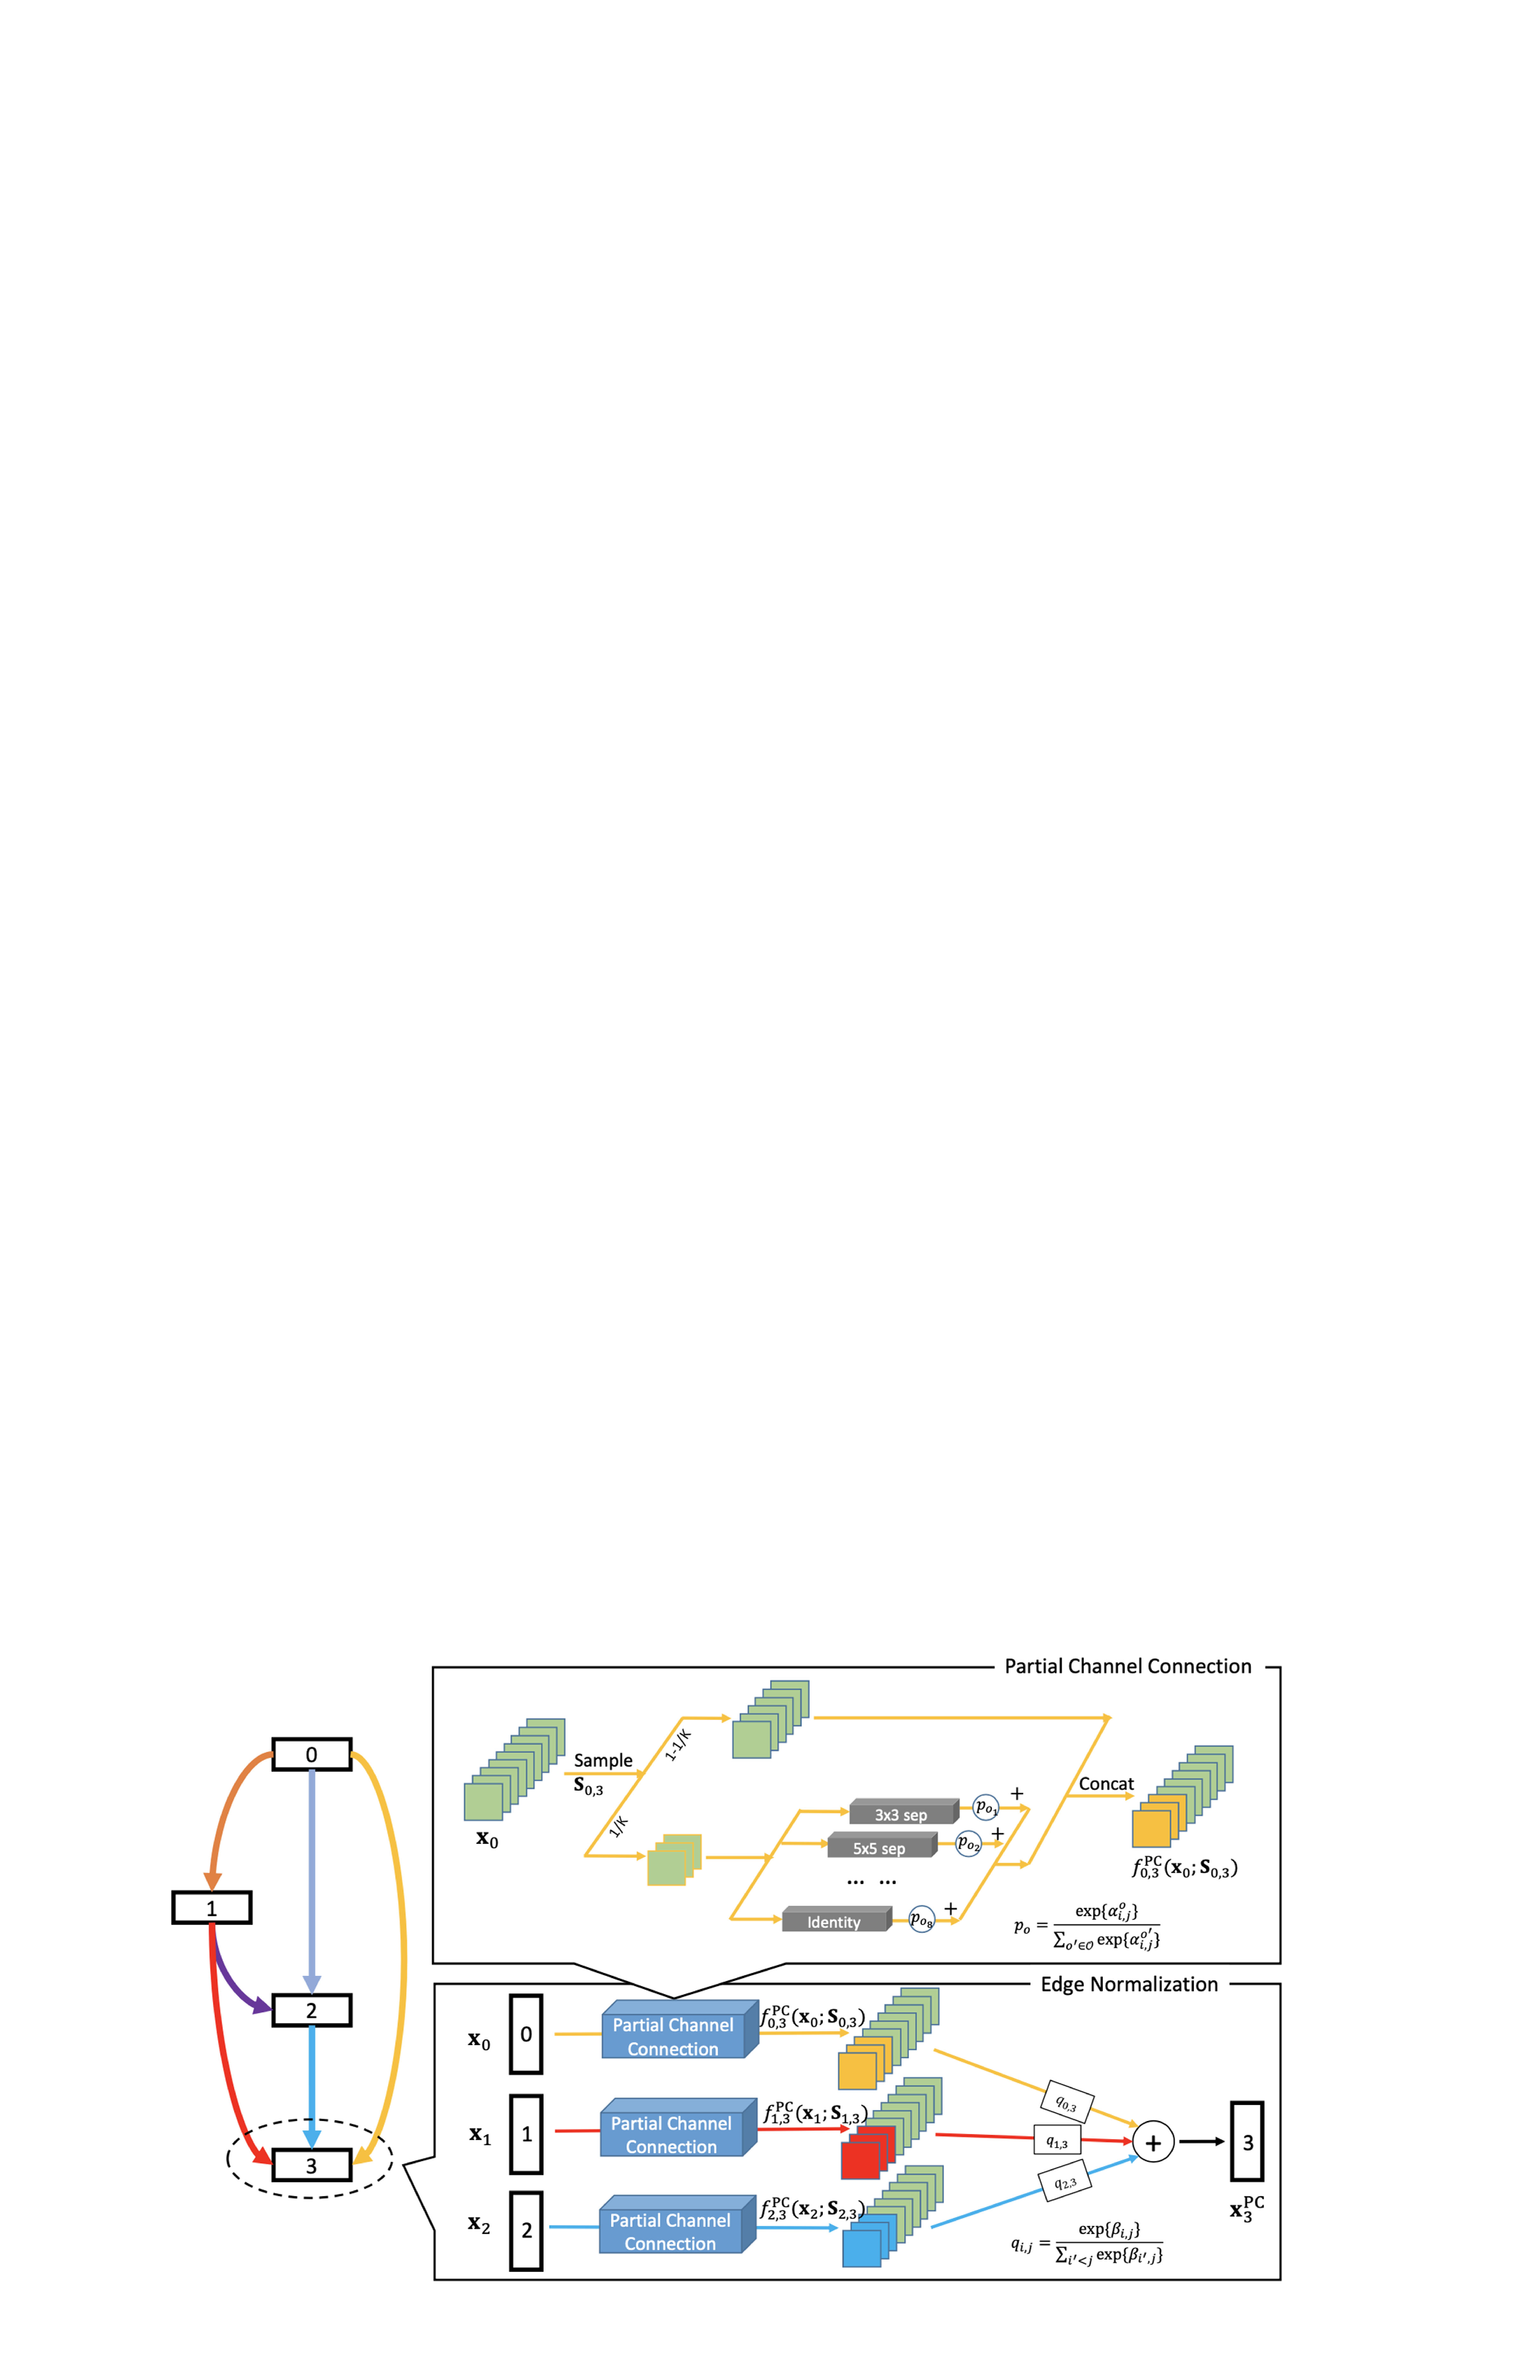
\includegraphics[width=0.52\textheight]{PC-DARTS.pdf}
	\caption{PC-DARTS算法流程\cite{3-7}}
	\label{fig1-10}
\end{figure}

基于EEG的NAS技术在近年来得到了一定关注。Li等人\cite{1-83}遵循基于强化学习的NAS\cite{1-79}设计思路,使用RNN作为控制器生成网络结构,并使用强化学习训练控制器使其逐步降低模型分类损失。其最终结果在两款情绪EEG的公开数据集上优于人工设计的CNN模型。Li等人\cite{1-84}将NAS策略与Transformer模型相结合,在NAS进程中兼顾模型的最终精度和空间复杂度,得到极具竞争力的情绪EEG辨识模型。Du等人\cite{1-85}利用多目标进化算法实现针对SSVEP范式EEG信号的NAS进程,并对生成的子网络应用网络模态(Network Morphism)和贝叶斯优化技术,以获取性能最优的搜索结果。Xue等人\cite{1-86}同样引入基于遗传算法的NAS模型,充分利用了遗传算法的启发式搜索和不需要梯度的优势来搜寻最优CNN架构。其结果证明,搜索得到的CNN模型能够在基于EEG的睡眠阶段分类任务中战胜当前最优算法。

从上述结果可知,尽管基于梯度的NAS模型具有相较于其他NAS算法更高的可解释性和更小的计算资源消耗,但是现有研究还并未将其迁移至EEG分类辨识领域。同时,现有算法针对单一范式EEG数据进行搭建,其泛化能力仍然存在提升空间。

\section{无监督域适应在脑电信号分析中的应用}
尽管现有方法已经在多种不同范式的EEG信号上取得了成功,但是基于MI范式的EEG信号分类仍然存在不小的难题。这主要归咎于以下问题:首先,MI信号采集时间短,样本数量少。相较于动辄数小时的情绪与睡眠EEG数据,MI的数据量难以驱动常规的深度学习模型;其次,MI无法利用外部刺激增强EEG响应幅度。相较于能够通过外部刺激诱发的SSVEP和ERP范式EEG信号,MI只能通过受试者本人的肢体运动想象诱发,EEG响应幅度与受试者本人生理状态息息相关。这直接造成了不同被试,甚至是同一被试在不同时间点上的特征差异;最后,MI范式的EEG信号其特征频段分布较窄,不同想象动作对应的活跃脑区也常常出现重叠现象,这进一步增加了模型的分类辨识难度。因此,相较于其他EEG范式,针对MI的研究的分类辨识效果仍相对较差\cite{1-51,1-59,1-71,1-75}。

近年来,无监督域适应(Unsupervised Domain Adaptation,UDA)算法在解决样本特征间具有较大方差的问题上崭露头角。无监督域适应通过将模型从标签信息丰富的源域迁移至标签稀疏的目标域,寻找对于域差异鲁棒的跨域模型。根据将源域表征迁移至目标域的原理,常见的无监督域适应算法可以分为以下几类:基于域间差异、基于对抗、基于域重构以及基于注意力机制\cite{1-89}。其中,基于域间差异的UDA通过计算并缩短源域和目标域网络对应激活层上的距离,应用统计学技术来减少域之间的差异\cite{1-90}。基于对抗的UDA通过搭建两个相互竞争的网络以实现对域不变特征的精准提取\cite{1-91}。基于域重构的UDA通过建立共享表示域,在保留源域和目标域特点的同时,拉近二者中样本的特征间距\cite{1-92}。基于注意力机制的UDA通过将源域中与目标域存在关联的部分进行迁移,引导网络关注源域数据中的域不变特征\cite{1-93}。UDA算法的基本思路如图\ref{fig1-11}所示,其消除源域和目标域的域间偏差,对齐两域中相同类别的样本,增大类间距离,并分离目标域中的未知类别。

\begin{figure}[!h]
	\centering
	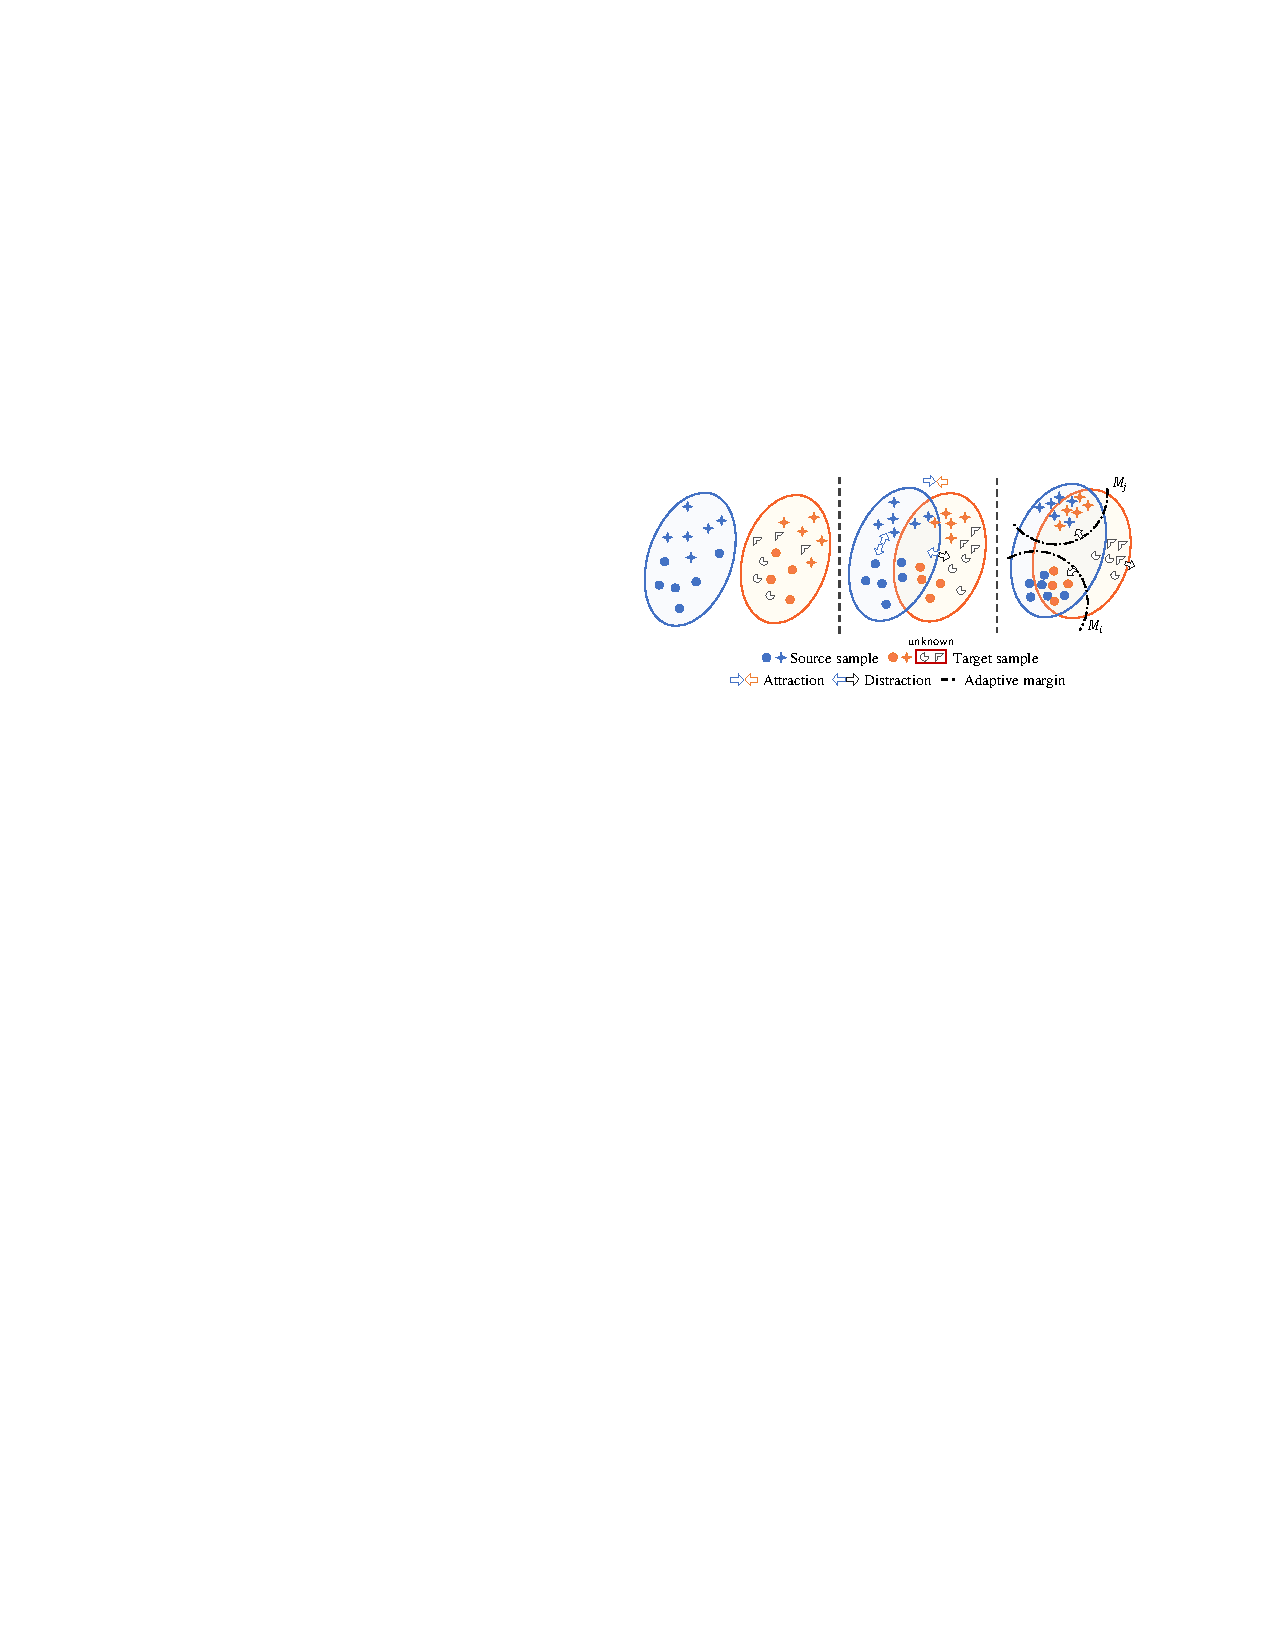
\includegraphics[width=0.52\textheight]{UDA.pdf}
	\caption{UDA算法思路\cite{1-94}}
	\label{fig1-11}
\end{figure}

考虑到基于MI范式的EEG信号存在的问题,无监督域适应算法便被应用到BCI领域中来。Chen等\cite{4-21}通过引入多注意力机制模块和域鉴别器,成功提取MI范式EEG数据的域不变特征,在三个不同公开数据集的跨时段MI辨识中取得了很好的效果。Hong等\cite{1-95}分别引入全局鉴别器和局部鉴别器对齐边缘分布,并降低条件分布差异。动态权重因子的引入使其能够有效权衡全局鉴别器和局部鉴别器的重要性,应对不同类型的数据分布。其的跨时段MI辨识分类取得了当时的最优结果。Tang等人\cite{1-96}提出了一种条件域自适应神经网络,从原始脑EEG时间序列中获取高分辨特征,其模型性能在更加严苛的跨被试MI场景下得到了验证。Zhang等人\cite{1-97}将EEG数据的协方差矩阵利用黎曼流形进行对齐,然后通过域适应算法最小化样本的联合概率分布。其在包含左手和右手两个类别的私人数据集上进行了性能验证,并击败了当时的最优算法。Zhu等人\cite{1-98}提出多源融合自适应正则化,结合加权平衡分布自适应,减少多源域间的域间差异。其挑选了公开MI数据集的左手想象和右手想象两个类别,验证了模型性能。

虽然这些方法取得了令人兴奋的结果,但是其中使用的UDA技术仍然需要改进,以应对更现实的MI应用场景。具体来说,在现实使用环境中,BCI系统常常面对同时跨被试和跨时段的应用要求,并且需要进行更多类别的分类辨识任务,这对BCI系统中的EEG解码算法提出了严峻挑战。



\section{本文的主要工作和创新点}
伴随着对大脑生理机制研究的不断深入,BCI系统的落地应用成为了可能。但是,现有基于EEG的BCI系统仍然在硬件和软件上存在着一定的不足,这制约了BCI系统在现实环境中的发展与推广。在硬件方面,当前市面上的高性能EEG采集设备存在着体积庞大,操作步骤复杂,价格昂贵的缺点,使其难以真正走入日常生活;消费级EEG采集设备又因为EEG通道数量较少,信号质量较差而限制了BCI的最终性能。因此,设计一款价格低廉,使用便捷,性能可靠,并且通道数量充足的EEG采集设备对BCI系统的发展具有重要的意义。同时,在软件方面,当前的EEG解码算法存在着结构设计困难,调参耗时以及泛化能力较差的问题。因此,本文配合采集设备,针对当前不同范式EEG信号的自身特点,对无需外部刺激诱发的被动范式和MI范式设计相应的EEG解码算法,有效推动BCI系统在情感分析、疲劳预警以及运动机能康复领域的应用。

针对当前BCI系统的不足,本课题分别从硬件和软件方面着手,设计并搭建了一套完整的BCI系统。其主要创新点如下:

(1) 本课题设计了一套基于EEG的BCI系统,命名为——JS-AINS-40。该系统的采集模块基于ARM微处理器和EEG集成前端芯片进行设计,能够以250 Hz-1000 Hz的采样率,同时采集40通道的EEG信号。为了尽可能降低采集系统中的噪声干扰,JS-AINS-40选型低噪声,高电源抑制比(Power Supply Rejection Ratio,PSRR)的供电芯片组成电源模块。同时,为了防止数字模块对模拟模块可能造成的干扰,在数字模块和模拟模块之间设计隔离模块。最后,为了提升设备在实际使用环境中的可靠性,在采集前端增加了低通滤波电路以消除EEG信号中的高频干扰,并在采集设备外露金属部分设计静电保护电路。在采集模块的硬件基础上,设计配套的下位机软件,并配合设计完成具有实时波形显示和数据保存功能的上位机软件。EEG采集硬件与下位机软件,上位机软件一同组成JS-AINS-40 BCI系统。设计完成后,本课题根据国标要求对JS-AINS-40系统进行了包括电压测量、共模抑制比测试、噪声电平测试以及电磁兼容性测试在内的性能检验,其结果符合国家标准。

(2) BCI系统的上位机不仅负责控制采集设备,接收EEG数据以及进行数据可视化,其还应具备EEG解码功能。本课题针对现有基于深度学习的EEG解码算法所存在的模型设计困难,参数调整耗时以及泛化能力不足问题,利用被动范式EEG数据量充足的优势,引入结合自适应机制和早停机制的神经结构搜索算法,成功实现了针对人脑情绪状态和疲劳状态的分类辨识。这是基于梯度的神经结构搜索技术在EEG领域的创新应用。为了验证模型的具体性能,本课题首先引入了基于情绪和疲劳的EEG公开数据集,并在其上取得了极具竞争力的分类结果。同时,为了进一步验证JS-AINS-40系统采集模块的性能,设计EEG情绪实验,并通过JS-AINS-40系统进行数据采集。最终的辨识结果验证了JS-AINS-40系统的可靠性。在两种不同类型被动范式EEG数据上的实验结果证明,所设计模型可以根据不同的数据集构建有针对性的网络架构,并具有针对基于EEG的心理生理状态识别任务的有效性和通用性。

(3) 本课题针对MI范式的EEG数据所具有的样本数量少,特征差异大问题,综合考虑MI-BCI系统所面临的使用情景,基于无监督域适应算法设计人脑运动意图辨识框架。这一框架融合动态迁移,伪标签自训练和迭代训练算法,成功实现了在MI数据上的跨被试同时跨时段分类。在三个公开MI数据集上的实验结果表明该框架具备优异的分类辨识性能。同时,配合JS-AINS-40系统,设计并进行MI实验。在JS-AINS-40所采集的数据集上的成功不仅进一步证明了所提出辨识框架的有效性,也证明了JS-AINS-40系统的可靠性。在四个MI数据集上,本课题验证了所提出框架的设计合理性,并对各模块的超参数选取进行了详细分析。

\section{本文工作的结构安排}

第一章~绪论

本章主要介绍了本课题的研究背景及意义,并从基于EEG的BCI系统基本结构和应用领域、EEG信号的基本特征,基于EEG的BCI系统典型范式以及国内外EEG采集设备的发展情况综合介绍基于EEG的BCI系统的研究现状。同时,本章还介绍了基于深度学习技术的EEG信号分析,以及深度学习的两个分支——神经架构搜索技术和无监督域适应算法的发展现状及其在EEG领域上的应用。最后,总结了本文的主要工作和创新点。

第二章~脑电信号采集系统设计

本章引入并介绍了JS-AINS-40系统。本章首先介绍了BCI系统应当具备的设计指标,并说明了JS-AINS-40系统的整体框架。其次,分别从硬件和软件两个方面展开介绍。硬件部分,本章首先介绍了JS-AINS-40系统的外观结构,并说明了其中两个组成部分——EEG采集盒和脑电极帽的外形参数。接下来,依次介绍了EEG采集盒中采集模块电路的各子模块器件选型以及电路设计。软件部分,本章分别介绍了JS-AINS-40系统的下位机软件设计流程以及上位机软件具体功能。最后,本章说明了对JS-AINS-40系统进行的性能测试,并展示了测试结果。

第三章~基于梯度自动优化的脑电辨识模型

本章介绍了JS-AINS-40系统配套的,针对被动范式中情绪和疲劳EEG的解码算法。首先,本章说明了根据EEG类型所引入的特征提取方法,介绍了所设计模型的基础架构,并在此基础上,详细说明了为了将基于图像的神经架构搜索技术迁移至EEG数据,所进行的针对性改进。其次,本章介绍了用来验证模型性能的情绪和疲劳两款公开数据集,以及用来验证JS-AINS-40可靠性的情绪数据集的具体采集流程。最后,本章分别介绍了所提出算法在三个数据集上搜索得到的最终模型架构,以及其分类辨识性能。通过与其他EEG辨识算法和神经架构搜索算法进行比较,验证了所提出模型的优异性。

第四章~基于多被试动态迁移与迭代自训练的脑电辨识算法

本章介绍了JS-AINS-40系统配套的,针对主动范式中MI类型EEG的解码算法。本章首先说明了常规算法在MI数据上存在的问题,申明了本章所提出框架的必要性。其次,定义了所提出框架应用的具体情景,并在此基础上详细介绍了框架的内部构成。接下来,本章说明了用来评估模型性能所使用的数据集,以及利用JS-AINS-40采集MI数据集的具体实验流程。除了数据集外,还介绍了所设计的对比算法,以及本章进行性能验证时的具体实验设定。紧接着,本章给出了所提出框架以及所有对比算法在四个MI数据集上的辨识结果,并对比了所有方法的复杂度。最后,通过大量的消融实验,本章证明了所提出框架设计的合理性,并对超参数选取进行了解释。

第五章~总结与展望

本章总结了全文的主要工作内容,并对未来该工作可能的研究方向进行展望。

\clearpage{\pagestyle{empty}\cleardoublepage}
% !Mode:: "TeX:UTF-8"

\chapter{脑电信号采集系统设计}

当前EEG采集设备高昂的价格、较大的设备体积以及复杂的操作流程是阻碍BCI系统推广的主要原因。如何在保证高质量EEG信号采集的同时,将采集设备的成本与体积控制在可接受范围内,并尽可能简化使用的复杂度,是BCI系统发展与落地的关键。针对这一问题,本章基于ARM微控制器设计了一款名为JS-AINS-40的BCI系统,其内部包含40通道的EEG采集设备,用于采集使用者的EEG信号,并可以对不同范式的EEG信号进行分析。

\section{JS-AINS-40系统性能指标}

在非侵入式BCI系统中,基于EEG信号的BCI系统由于能够捕获人脑神经细胞群自发的、节律性的电活动,具有极高的时间分辨率和较低的使用成本而得到了最广泛的应用。EEG中蕴含的大量神经影像学信息,能够为疾病诊断、人脑功能认知以及人脑状态辨识提供有力支撑。然而,EEG作为一种低幅值,低信噪比以及低频率的生理电信号,其采集难度极高。同时,EEG信号也是一种具有空间相干性的随时间快速变化的非线性生理电信号,其采集过程需要较高的空间采样率\cite{2-1}。综上所述,EEG采集仪器应当是一种具有高灵敏度、低响应延迟,能够保留信号空间相干性并可以抑制外来噪声干扰的多导联设备\cite{2-2}。

遵循上述内容,一个合格的EEG信号采集设备应当在设计时考虑以下性能指标\cite{2-3}:

(1) 输入阻抗。EEG信号作为一种微弱的生理电信号,其幅值集中在0-200 $\mu$V之间。同时,人脑头皮与EEG电极之间通常具有极高的阻抗值。这一阻抗值还会随着受试者的生理状态波动,导电介质(脑电极膏或者生理盐水)损耗,以及人脑头皮与EEG电极之间的相对位置变化而不断浮动。这导致了EEG信号采集设备需要具备尽可能高的输入阻抗值。否则人脑头皮与EEG电极之间的阻抗变化将会对EEG信号的低频段产生极大的干扰,影响整个采集过程。

(2) 共模抑制比。采集设备通常工作在充满工频干扰信号的使用环境中。$50$ Hz工频干扰信号常常以共模噪声的形式进入采集设备,混杂进EEG信号之中。极端情况下,干扰信号的幅值大小甚至会超过EEG信号,使得EEG信号淹没在噪声之中。为了提高所采集信号的质量,减少共模噪声对采集过程带来的干扰,要求EEG采集设备具有较高的共模抑制比。通常情况下,要求EEG采集设备的共模抑制比大于$90$ dB。

(3) 频率响应范围。由于EEG信号的频率范围通常在100 Hz以内,因此采集设备在采集100 Hz以内不同幅值的信号时,应当保证信号不产生失真现象。

(4) 增益大小。由于EEG信号幅值较低的特性,其难以直接被A/D芯片正常采集。因此,需要在保证不失真的前提下对信号进行放大,以保证采集过程的有效进行。

(5) 线性误差值。脑电设备应该具有尽可能小的线性误差,以保证实际输出值和理论值之间的偏差处于可接受范围,防止测量误差对人脑辨识结果造成不利影响。


\section{JS-AINS-40系统总体设计方案}


\begin{figure}[!h]
	\centering
	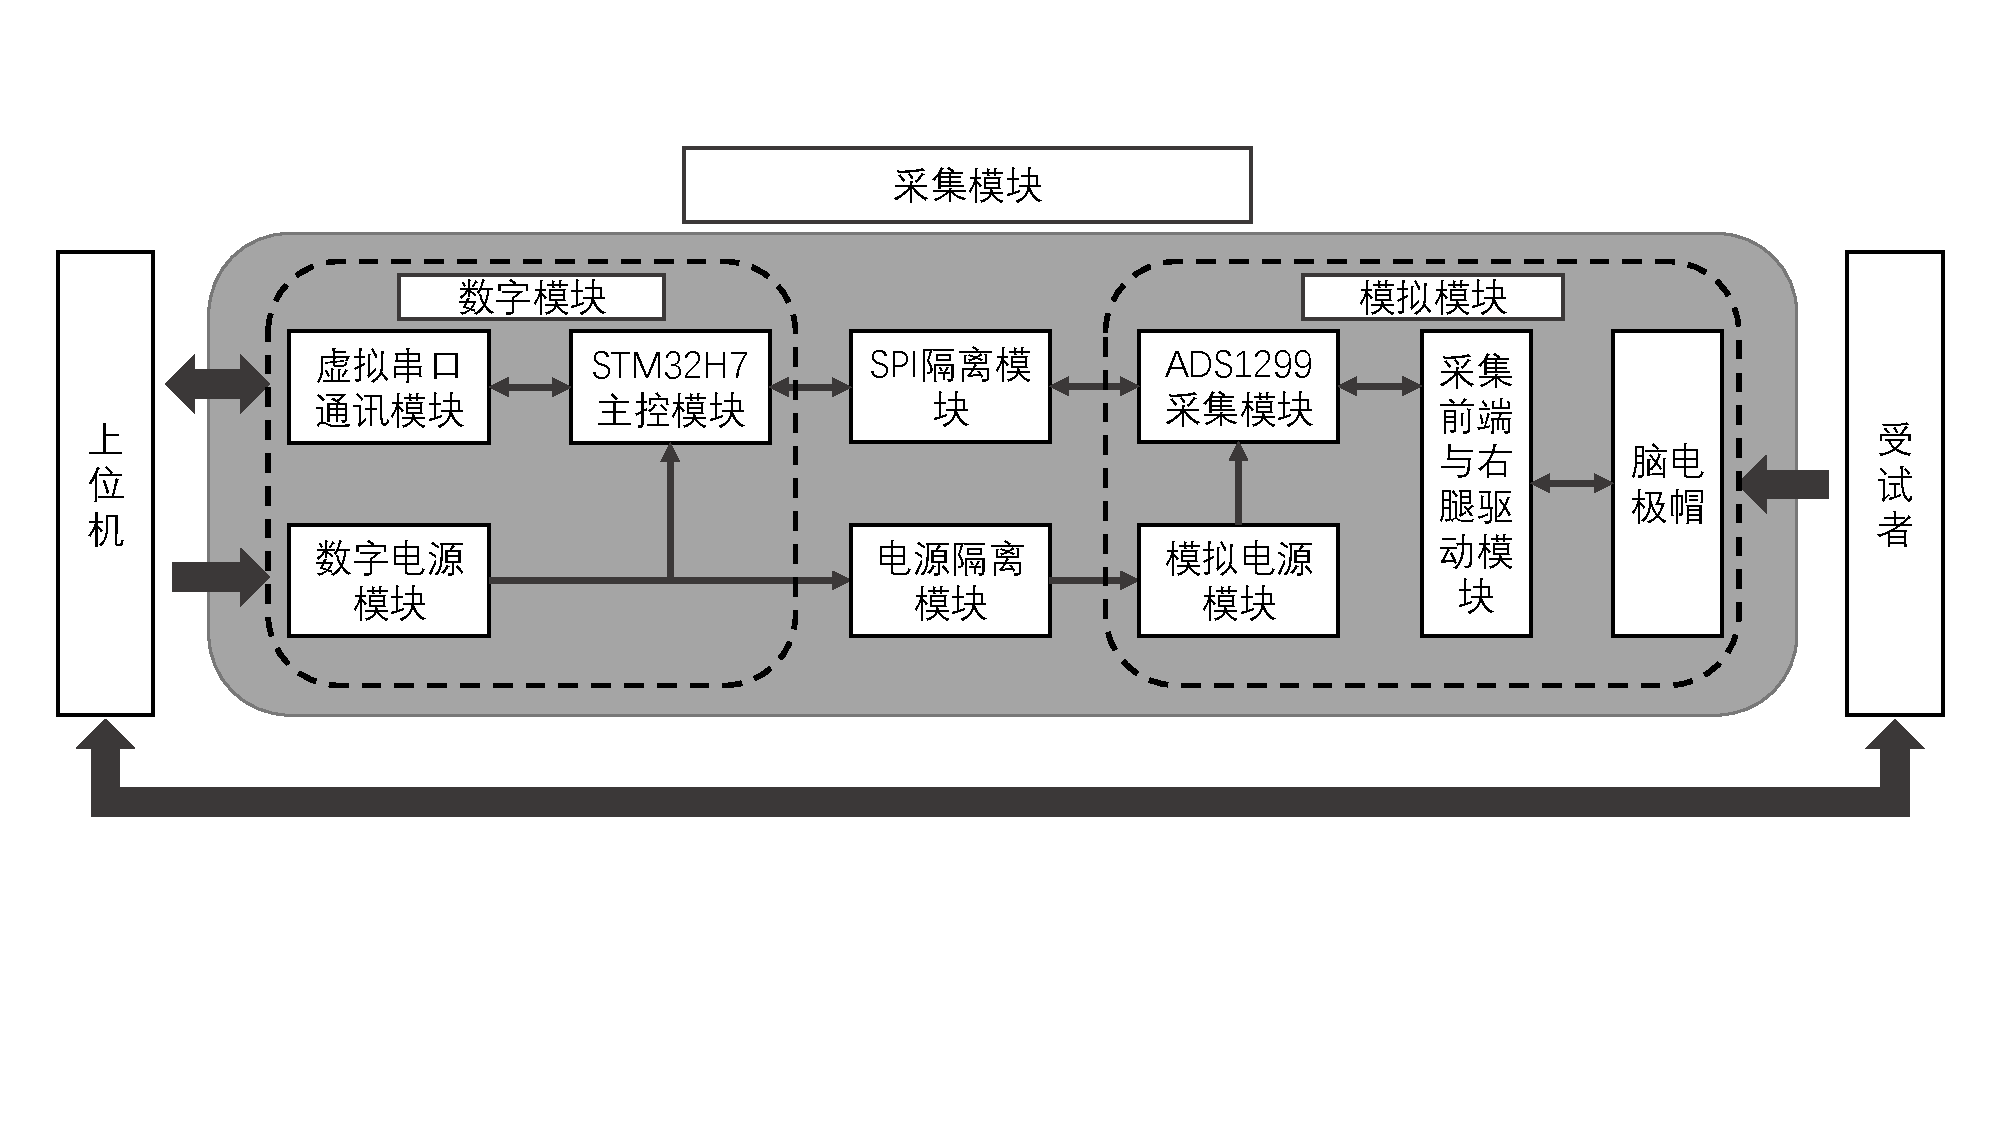
\includegraphics[width=0.60\textheight]{系统总体结构.pdf}
	\caption{JS-AINS-40系统总体结构}
	\label{fig2-1}
\end{figure}
JS-AINS-40系统的总体结构如图\ref{fig2-1}所示。其主要包含三个相互关联的不同组成部分:上位机、受试者以及中间的采集模块。其中,采集模块的设计是本节的描述重点。采集模块包括:虚拟串口通讯模块、数字电源模块、STM32H743IIT6主控模块、SPI隔离模块、电源隔离模块、ADS1299采集模块、模拟电源模块、采集前端与右腿驱动模块以及脑电极帽。其中虚拟串口通讯模块、数字电源模块与STM32H743IIT6主控模块属于数字模块。ADS1299采集模块、模拟电源模块、采集前端与右腿驱动模块以及脑电极帽属于模拟模块。

所有模块的具体工作流程如下:首先,上位机运行相应的实验程序,对受试者进行相应范式的EEG诱发。受试者产生的EEG信号被脑电极帽采集,经过采集前端与右腿驱动模块处理后以模拟信号的形式进入ADS1299采集模块。ADS1299采集模块将模拟信号转换为相应的数字信号,携带相应的设置字符串发送给STM32H743IIT6主控模块。STM32H743IIT6主控模块对数字信号进行排序与裁剪后,将处理后的数据通过虚拟串口模块发送给上位机。整个采集模块由上位机进行供电。需要注意的是,数字模块与模拟模块之间通过SPI隔离模块与电源隔离模块对信号通讯与电源传输进行隔离,防止数字模块的噪声对模拟信号采集造成影响。

\section{JS-AINS-40系统采集模块硬件结构设计}
JS-AINS-40系统的采集模块外观如图\ref{fig2-22}(a)所示。在物理结构上,其可以划分为两个组成部分,EEG采集盒和脑电极帽。
\vspace{6mm}

\begin{figure}[!h]
	\centering
	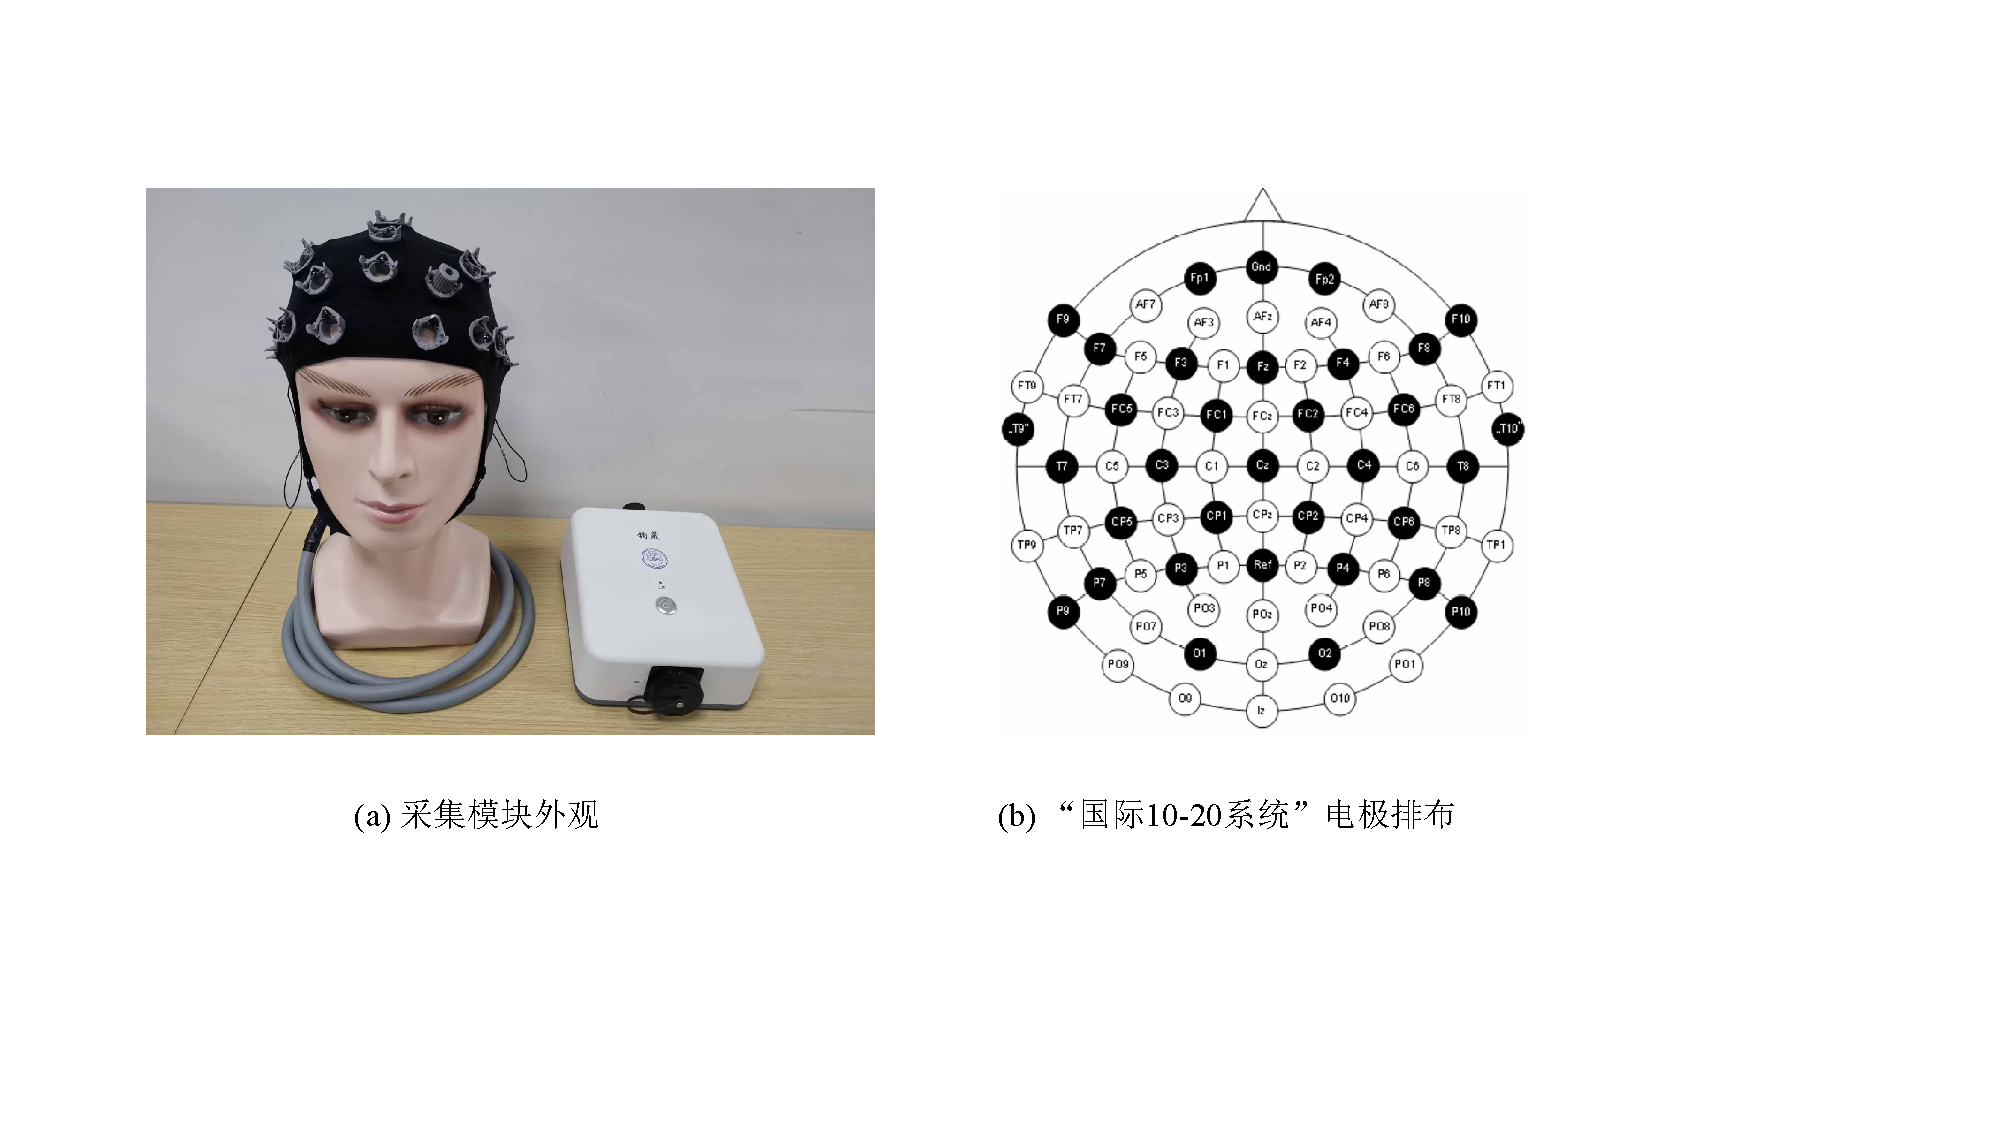
\includegraphics[width=0.6\textheight]{10-20.pdf}
	\caption{采集模块结构外观}
	\label{fig2-22}
\end{figure}

EEG采集盒体积为19.7 cm $ \times $ 15.8 cm $ \times $ 3.6 cm(长$\times$宽$\times$高),其作为采集模块的核心部件,内部包括采集模块PCB、用来固定PCB的安装立柱、LED导光柱、设备启动按钮、用来传输数据和给设备供电的USB接口以及用来连接脑电极帽的航空插头。

脑电极帽上的电极排布一般遵循“国际10-20系统”,标准的“国际10-20系统”如图\ref{fig2-22}(b)所示。自主设计的脑电极帽根据使用场景需求,选取“国际10-20系统”中的40个不同电极:FP1,FP2,AF7,AF3,AFz,AF4,AF8,F7,F3,Fz,F4,F8,FT7,FC3,FCz,FC4,FT8,T7,C3,Cz,C4,T8,TP7,CP3,CPz,CP4,TP8,P7,P3,Pz,P4,P8,PO7,PO3,POz,PO4,PO8,O1,Oz,O2,‘T9’,‘T10’。

其中‘T9’,‘T10’分别代表位于左耳后乳突的参考电极和右耳后乳突的右腿驱动电极。本设备可以同时对40个通道的EEG信号以最高1 kHz的速率进行采集,采集模块的具体设计将在后面章节详细介绍。

\section{JS-AINS-40系统采集模块硬件电路设计}

JS-AINS-40系统中的采集模块PCB实物图如图\ref{fig2-4}所示(为了方便展示,图中去除了屏蔽罩和排线),图中用不同颜色的框线标注出了各子模块的位置。在上述总体设计方案的基础上,本章详细叙述各个模块的器件选型与内部电路设计。
\begin{figure}[h!]
	\centering
	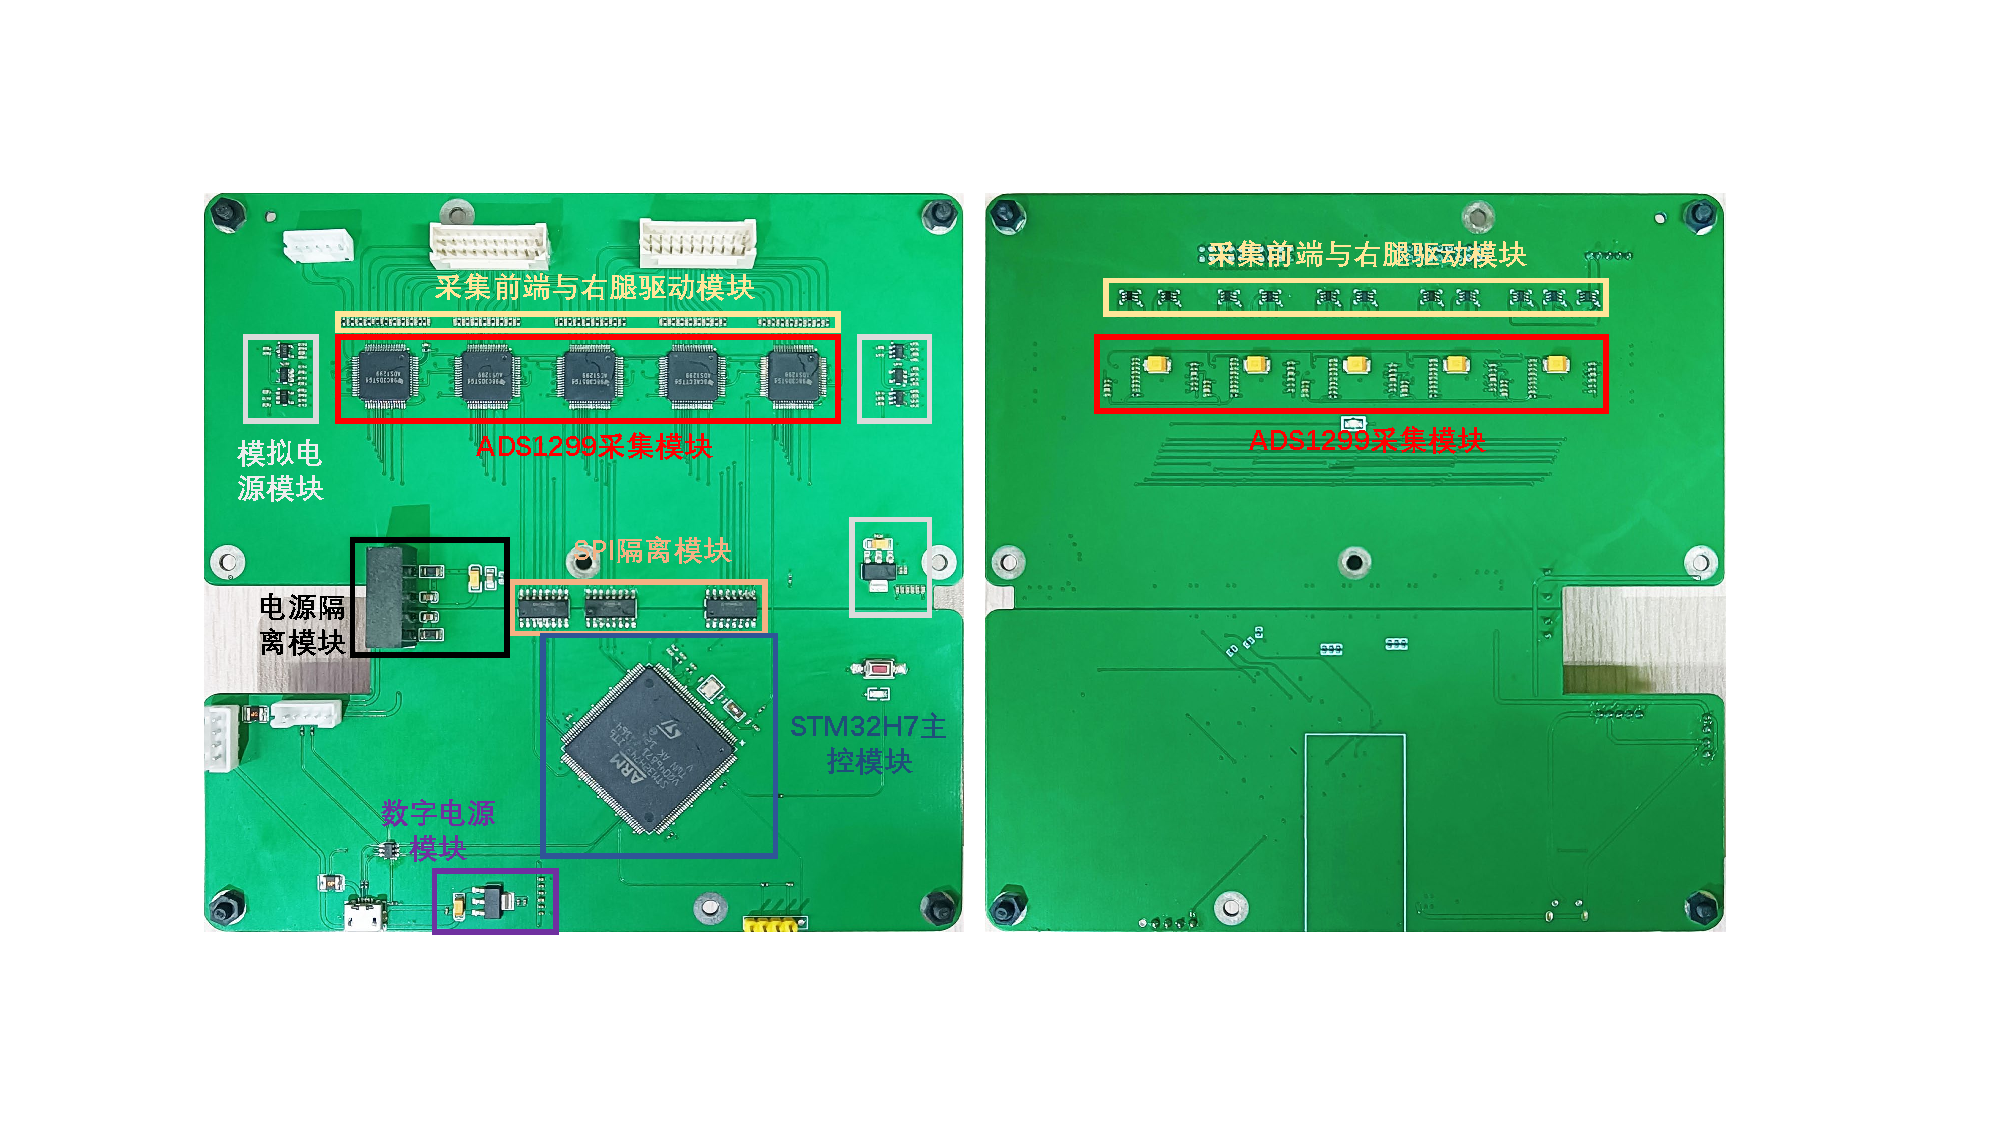
\includegraphics[width=0.50\textheight]{PCB实物图.pdf}
	\caption{JS-AINS-40系统采集模块PCB实物图}
	\label{fig2-4}
\end{figure}

毫无疑问,元器件的选型决定了设备性能的上限,而核心模块内部的芯片选型则是整个设计的重中之重,它决定了设备能否满足设计指标。因此,在开始具体的说明之前,首先对核心芯片进行介绍。采集模块中的数字模块与模拟模块分别围绕两个核心芯片构建,所有的外围模块均服务于这两个核心组件。
% \begin{figure}[!h]
% 	\centering
% 	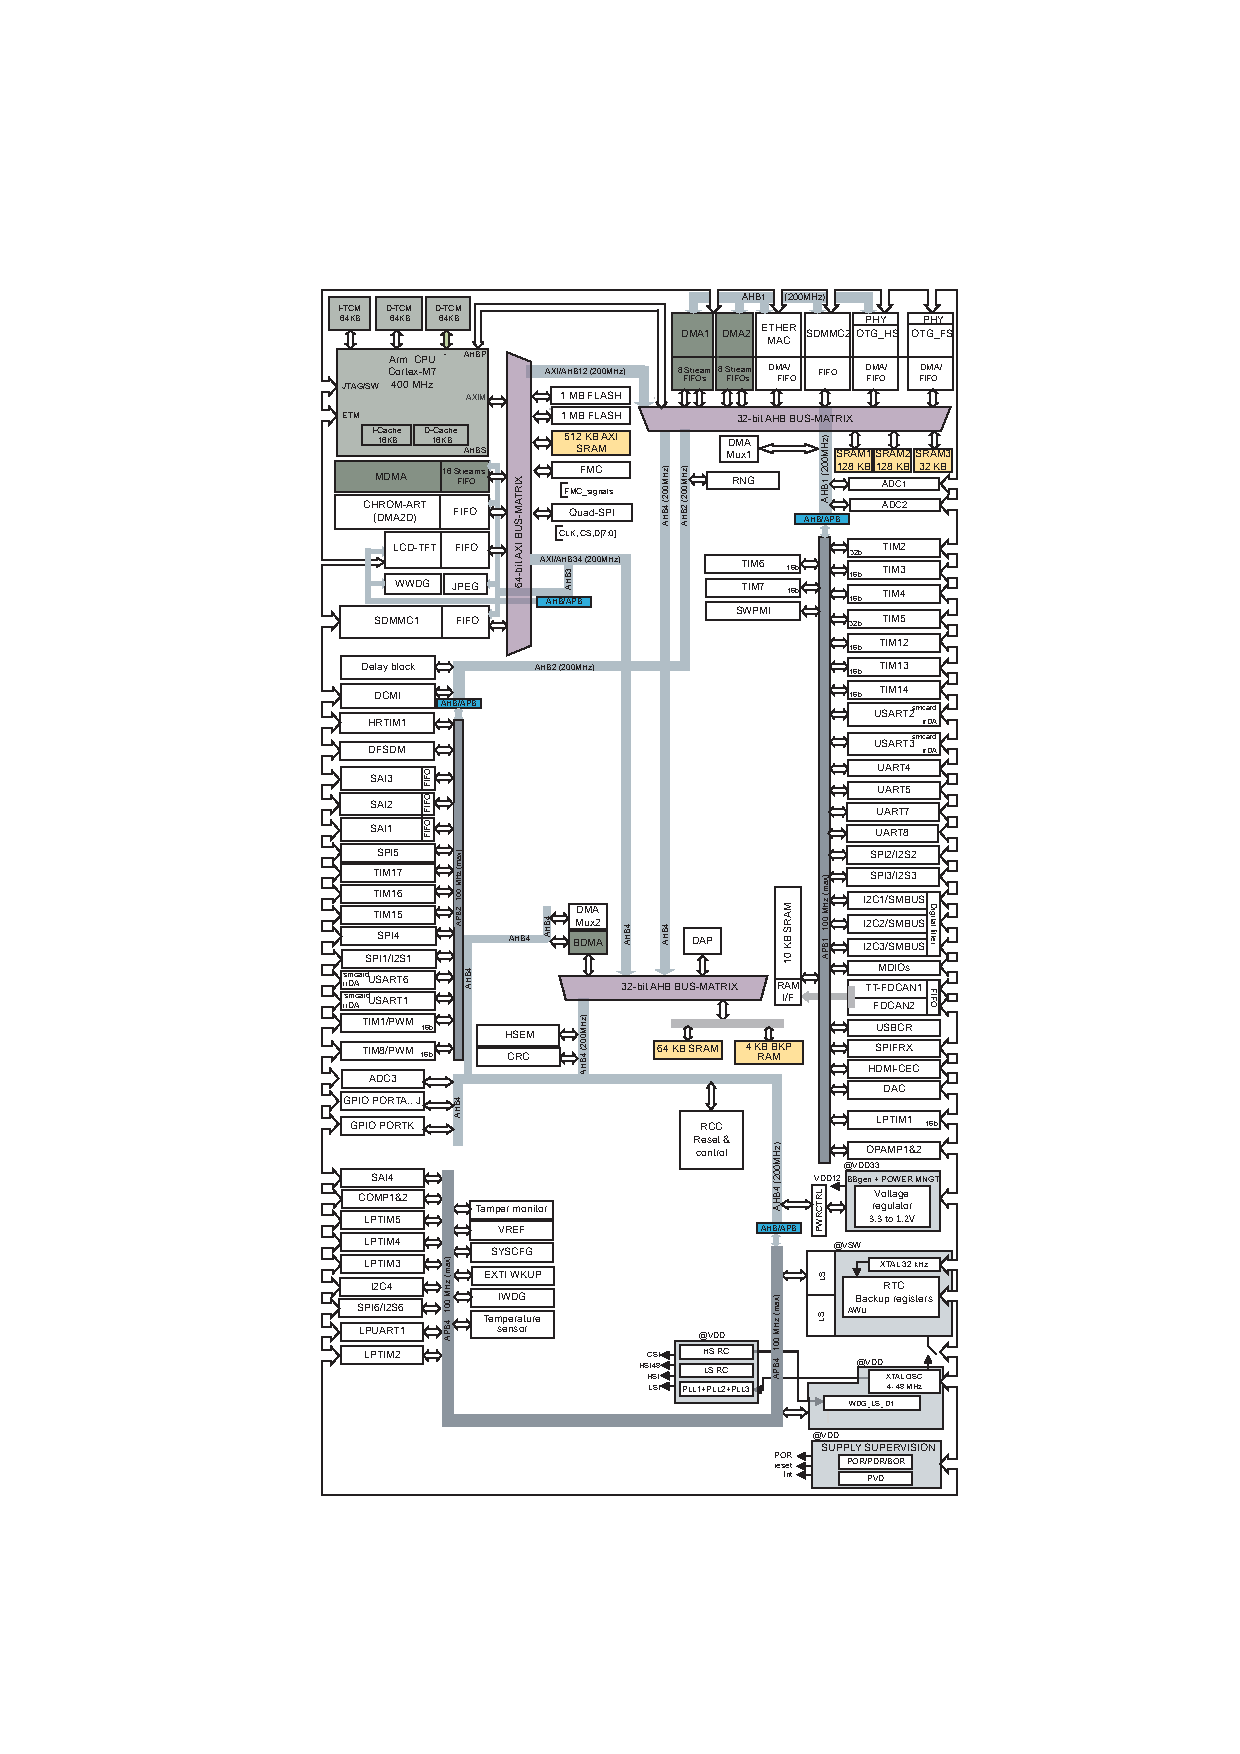
\includegraphics[width=0.44\textheight]{芯片资源_32.pdf}
% 	\caption{STM32H743IIT6内部资源展示}
% 	\label{fig2-3}
% \end{figure}
数字模块的核心选取意法半导体公司出品的STM32系列中的H743IIT6芯片。其内部的32位ARM Cortex-M7内核具有双精度FPU以及L1高速缓存(16 KB的数据缓存和16 KB的指令缓存),主频达到480 MHz,能够为40导联EEG采集设备提供所需的高速数据处理。同时,该芯片包含2 MB的闪存,1 MB RAM,168个高速(133 MHz)I/O口,4个DMA控制器,22个定时器以及大量的通讯与模拟外设。这些设备能够为40通道EEG数据提供足够的存储空间,满足主控芯片同时与多块采集芯片进行通信的需求。%STM32H743IIT6内部结构如图\ref{fig2-3}所示。
\begin{figure}[!h]
	\centering
	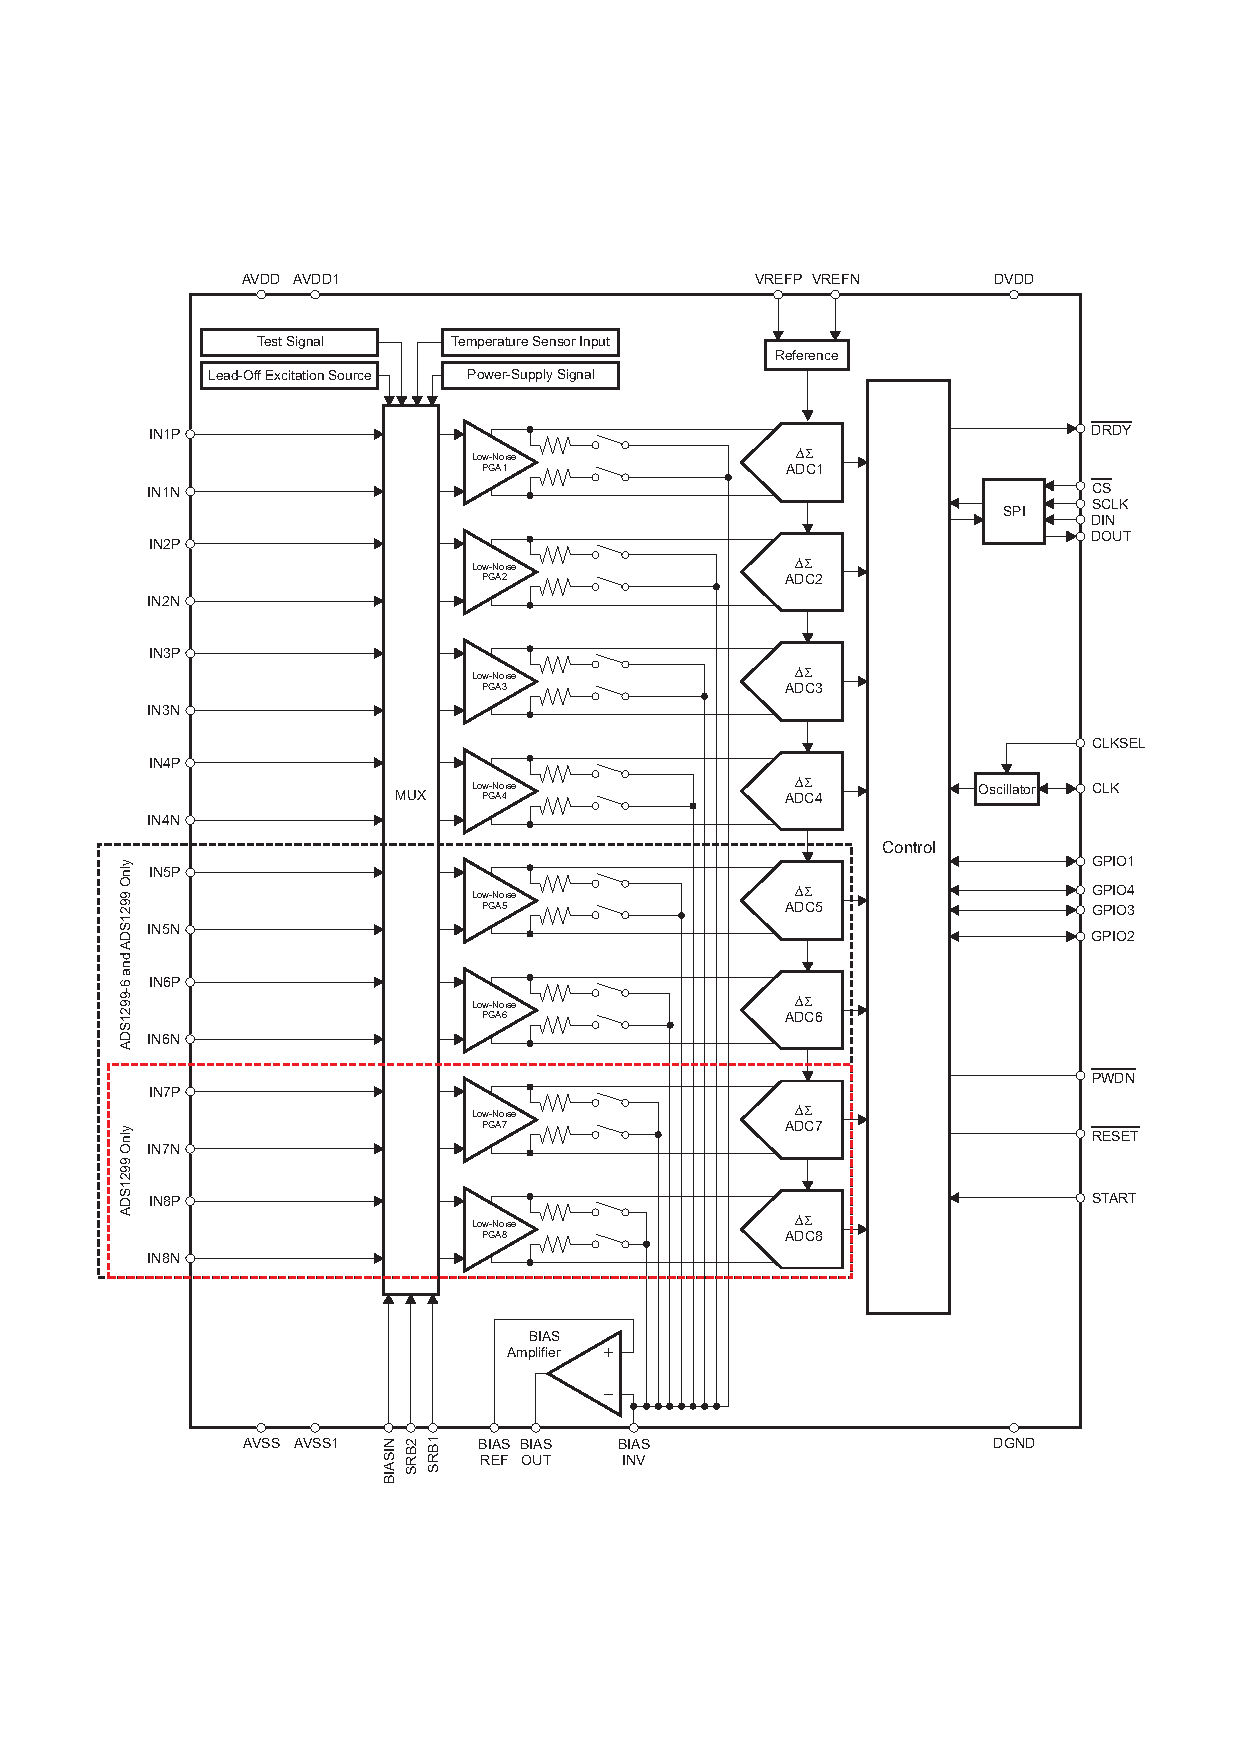
\includegraphics[width=0.50\textheight]{芯片资源_1299.pdf}
	\caption{ADS1299内部结构示意图}
	\label{fig2-2}
\end{figure}

模拟模块的核心是德州仪器公司设计的低噪声生物电势测量芯片——ADS1299。作为一款专用的8通道24位模数转换器,其内部结构如图\ref{fig2-2}所示。ADS1299内部的八个通道能够实现高分辨率下的24位同步采样,并且每个通道还配套了对应的可编程增益放大器(Programmable Gain Amplifier,PGA)。该芯片能够在任意输入通道生成患者的偏置输出信号(右腿驱动功能),并自主选取反馈连接方式。此外,该芯片还能够在–40$^{\circ}$C至+85$^{\circ}$C的工作环境下,以250 Hz至16 kHz的采样率完成EEG信号采集工作,完全满足当前EEG采集任务的要求。ADS1299作为一款成熟的EEG采集芯片,其设计高度集成化,性能可靠且能够满足EEG采集设备的设计指标,因此本章以其作为模拟模块的核心。

\subsection{电源模块设计}

电源模块为整个系统提供能源保障,是系统能够正常工作的“根基”。电源模块在设计时需要充分考量设备的具体能耗,并留出充足的裕量以应对特殊情况。如果电源的参数选取不合理,轻则导致设备无法长时间稳定工作,重则造成设备损毁,危及使用者安全。兼顾设备性能与元器件成本的电源设计,将是整个系统设计的基础。JS-AINS-40系统采集模块的电源包括数字电源模块与模拟电源模块。

采集模块使用上位机PC端的USB端口为整个模块供能,大幅简化了设备使用条件。但与此同时,PC端因为直接接入220 V市电电网,毫无疑问会具有较大的噪声干扰。尽管这些干扰不会影响PC的正常运行,但对于采集微弱EEG信号的采集模块,这些噪声的存在将会是毁灭性的。因此,本章在设计时将数字电源模块与模拟电源模块进行隔离。

(1) 数字电源模块设计

数字电源模块为采集模块中的虚拟串口通讯模块、STM32H743IIT6主控模块和SPI隔离模块的数字侧供能。上述模块均工作在直流3.3 V电压下,而USB端口只能提供直流5 V供电,因此需要数字电源模块进行电压转换。同时,考虑到数字模块对噪声具有较强的鲁棒性,本节选取德州仪器生产的TLV1117-33CDCYR芯片将PC的5 V供电转换为3.3 V,并直接提供给数字模块使用。实验证明,这一设计符合性能需求。TLV1117-33CDCYR是一款正输出低压差线性稳压器(Low-Dropout Regulator,LDO),能够为负载提供800 mA的电流输出。该LDO在输入电压与输出电压压差达到1.2 V以上时即可正常工作、具有较好的纹波表现,并且仅需设计简单的外围电路。上述优点促使本节选取其作为数字模块供电芯片。图\ref{fig2-5}展示了TLV1117-33CDCYR的原理图。

\begin{figure}[!h]
	\centering
	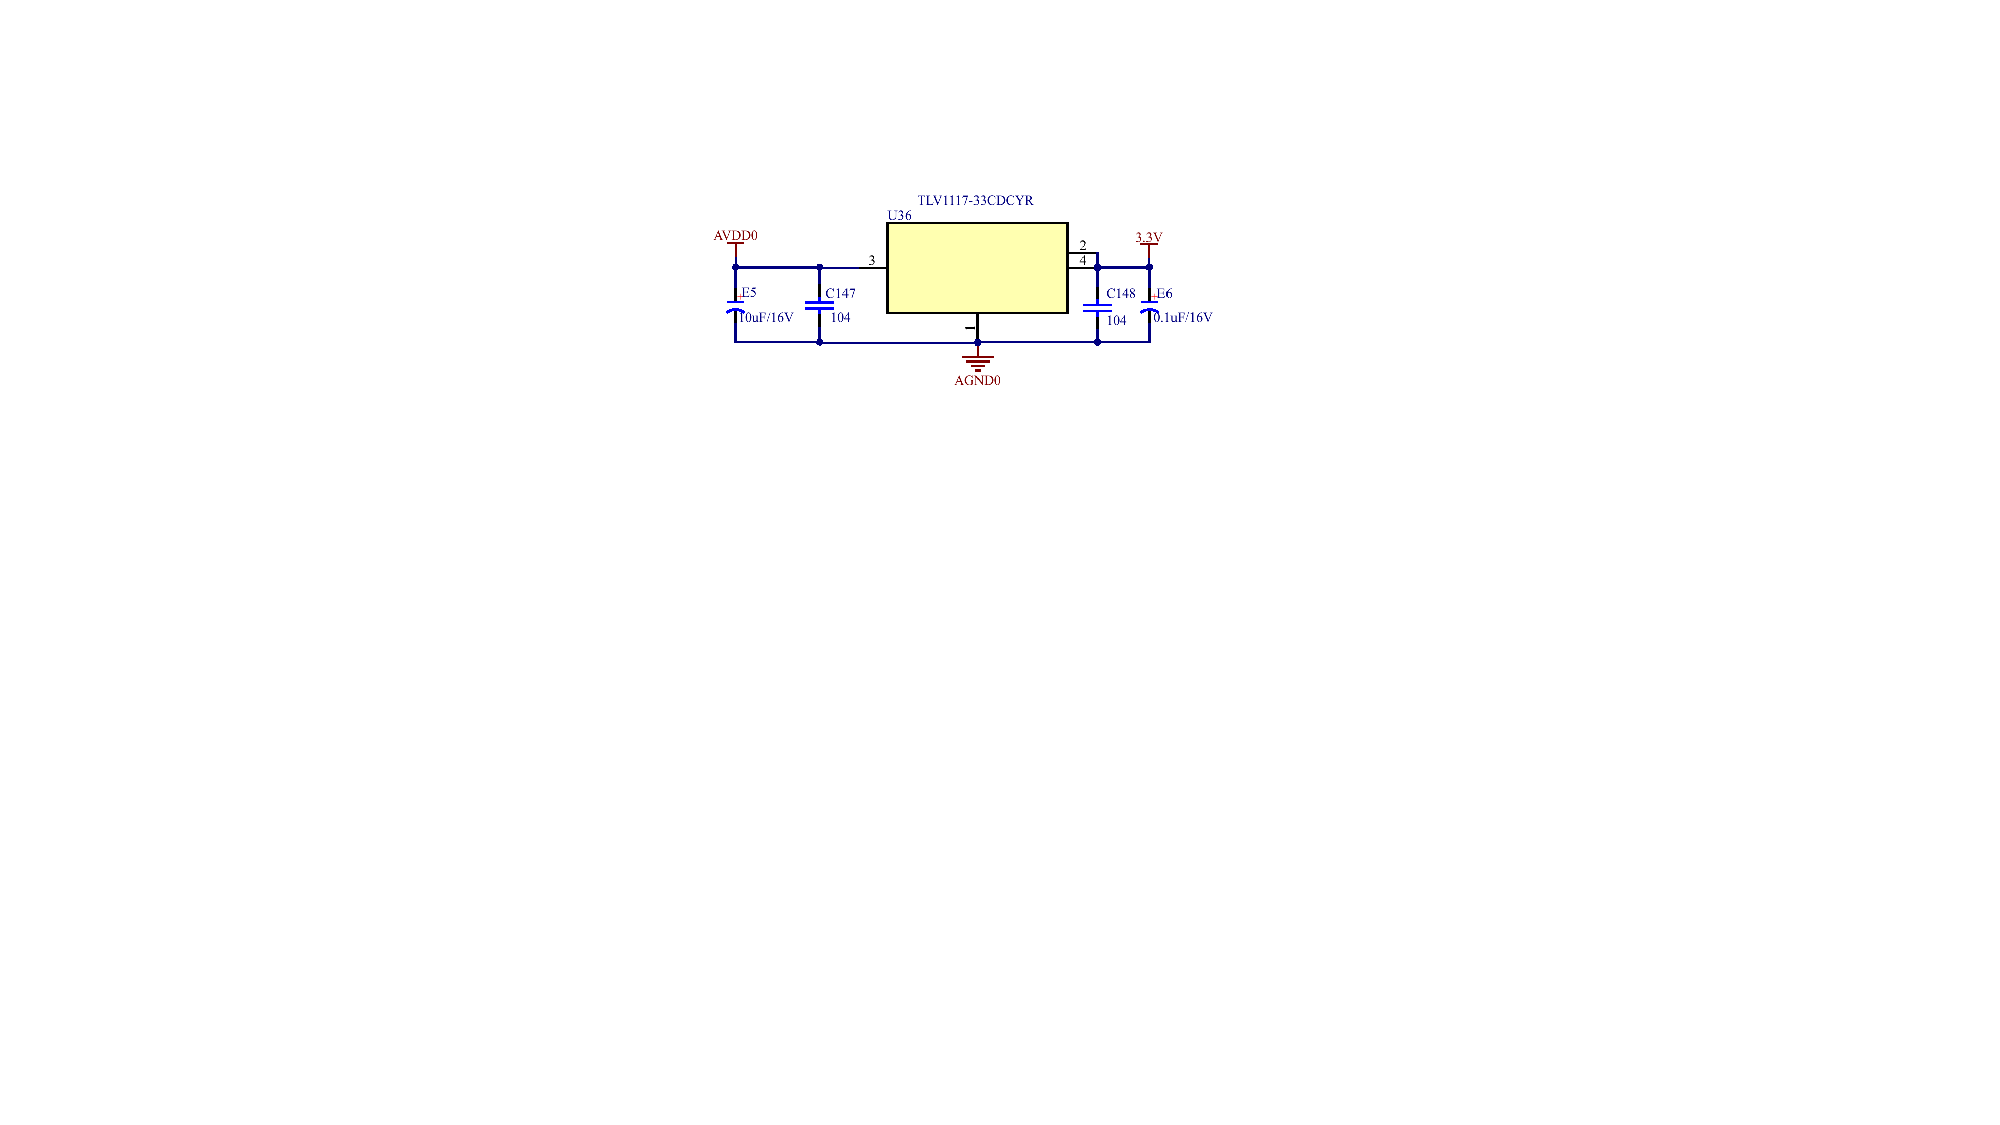
\includegraphics[width=0.46\textheight]{数字1117.pdf}
	\caption{TLV1117-33CDCRY原理图}
	\label{fig2-5}
\end{figure}

(2) 电源隔离模块设计

\begin{figure}[!h]
	\centering
	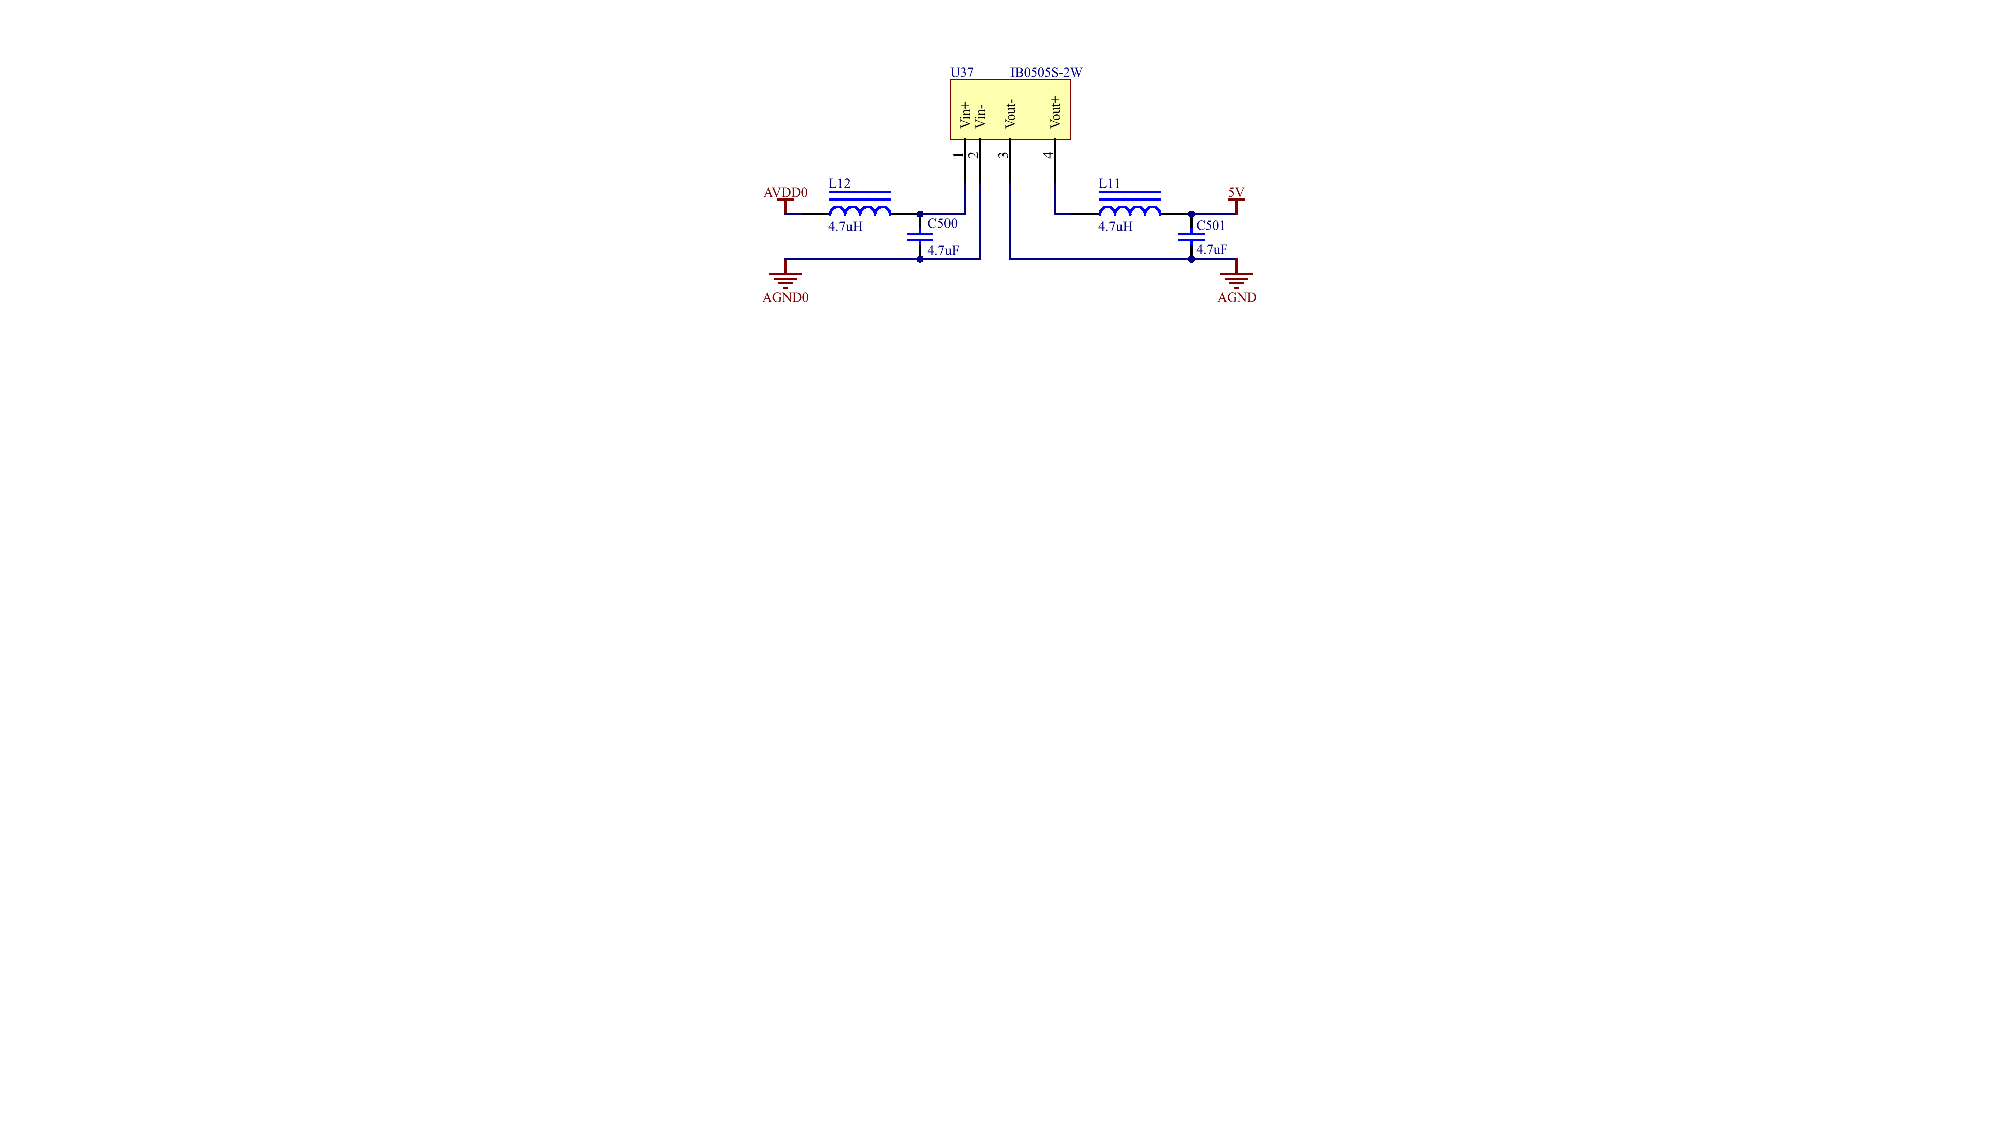
\includegraphics[width=0.46\textheight]{DCDC.pdf}
	\caption{IB0505S-2W原理图}
	\label{fig2-6}
\end{figure}

为了提升JS-AINS-40系统的安全性,并隔离数字端可能存在的噪声干扰,在数字电源模块与模拟电源模块之间添加电源隔离模块。综合考虑使用场景,引入金升阳公司的DCDC模块电源IB0505S-2W进行电源隔离。其具备较小的体积、与ADS1299相近的适用温度、良好的温度特性、1000 VDC的隔离能力、最大2 W的输出功率以及80\%的转换效率,满足模拟模块的使用要求。本节将USB端口的5 V供电输入IB0505S-2W,其输出的5 V电压作为模拟模块的电源。IB0505S-2W的相关电路如图\ref{fig2-6}所示。

(3) 模拟电源模块设计

模拟电源模块为ADS1299采集模块、SPI隔离模块的模拟侧以及采集前端与右腿驱动模块供电。根据ADS1299的设计需求,本章选择双极电源为其供电。分别为ADS1299的AVDD引脚提供$\rm +2.5$ V的模拟正电源,AVSS引脚提供$\rm -2.5$ V的模拟负电源以及DVDD引脚提供3.3 V的模拟电源。由于本章设计使用ADS1299的内部参考电压,而内部参考电压基于AVSS生成。内部参考电压$\mathrm{~V}_{\mathrm{REF}}$的大小直接影响了ADS1299信号幅值测量的准确性:

\begin{equation}
    \label{deqn_ex2_1}
\text{量程范围} =\frac{\pm \mathrm{V}_{\mathrm{REF}}}{\text { Gain }}=\frac{2 \mathrm{~V}_{\mathrm{REF}}}{\text { Gain }}
\end{equation}
其中$\text{Gain}$为ADS1299的内部PGA增益。因此,模拟电源模块的供电芯片,特别是AVSS引脚的$\rm -2.5$ V供电芯片需要专门挑选低纹波线性稳压器。

本节设计的具体选型如下:将电源隔离模块IB0505S-2W输出的5 V供电作为电源,分别传递给TLV1117-33CDCRY、TPS60403DBVR和TPS73225DBVR。TLV1117-33CDCRY已经在数字电源模块使用过一次,不再详细介绍。其输出的3.3 V为ADS1299的DVDD供电。TPS60403DBVR是德州仪器公司生产的一款电荷泵电压逆变器,其能够以90\%的效率将输入转化为负输出电压,并为负载提供60 mA的电流。本节中,使用TPS60403DBVR将5 V转化为-5 V,提供给TPS72325DBVR。TPS72325DBVR是德州仪器公司生产的低噪声、高电源抑制比的负输出线性稳压器。其输出噪声低于60 $\mu V_{RMS}$,电源抑制比在$1$ kHz时为$65$ dB,内部提供短路与过载检测保护装置,符合当前的设计要求。因此,本节使用TPS72325DBVR将-5 V转化为-2.5 V作为输入传递给ADS1299的AVSS。TPS73225DBVR同样来自德州仪器公司,是一款低噪声线性稳压器。其输出噪声低于30 $\mu V_{RMS}$,电源抑制比在$1$ kHz时为$55$ dB,内部提供反向电流保护装置,符合当前的设计要求。本节使用TPS73225DBVR将5 V转化为2.5 V提供给ADS1299的AVDD。为保证设备可靠运行,设计两组相同的供电电路分别为一半数量的ADS1299供能,两组电源能够提供的功率为600 mW,远高于模拟模块所需总功率。整个设计如图\ref{fig2-7}所示。

\begin{figure}[h]
	\centering
	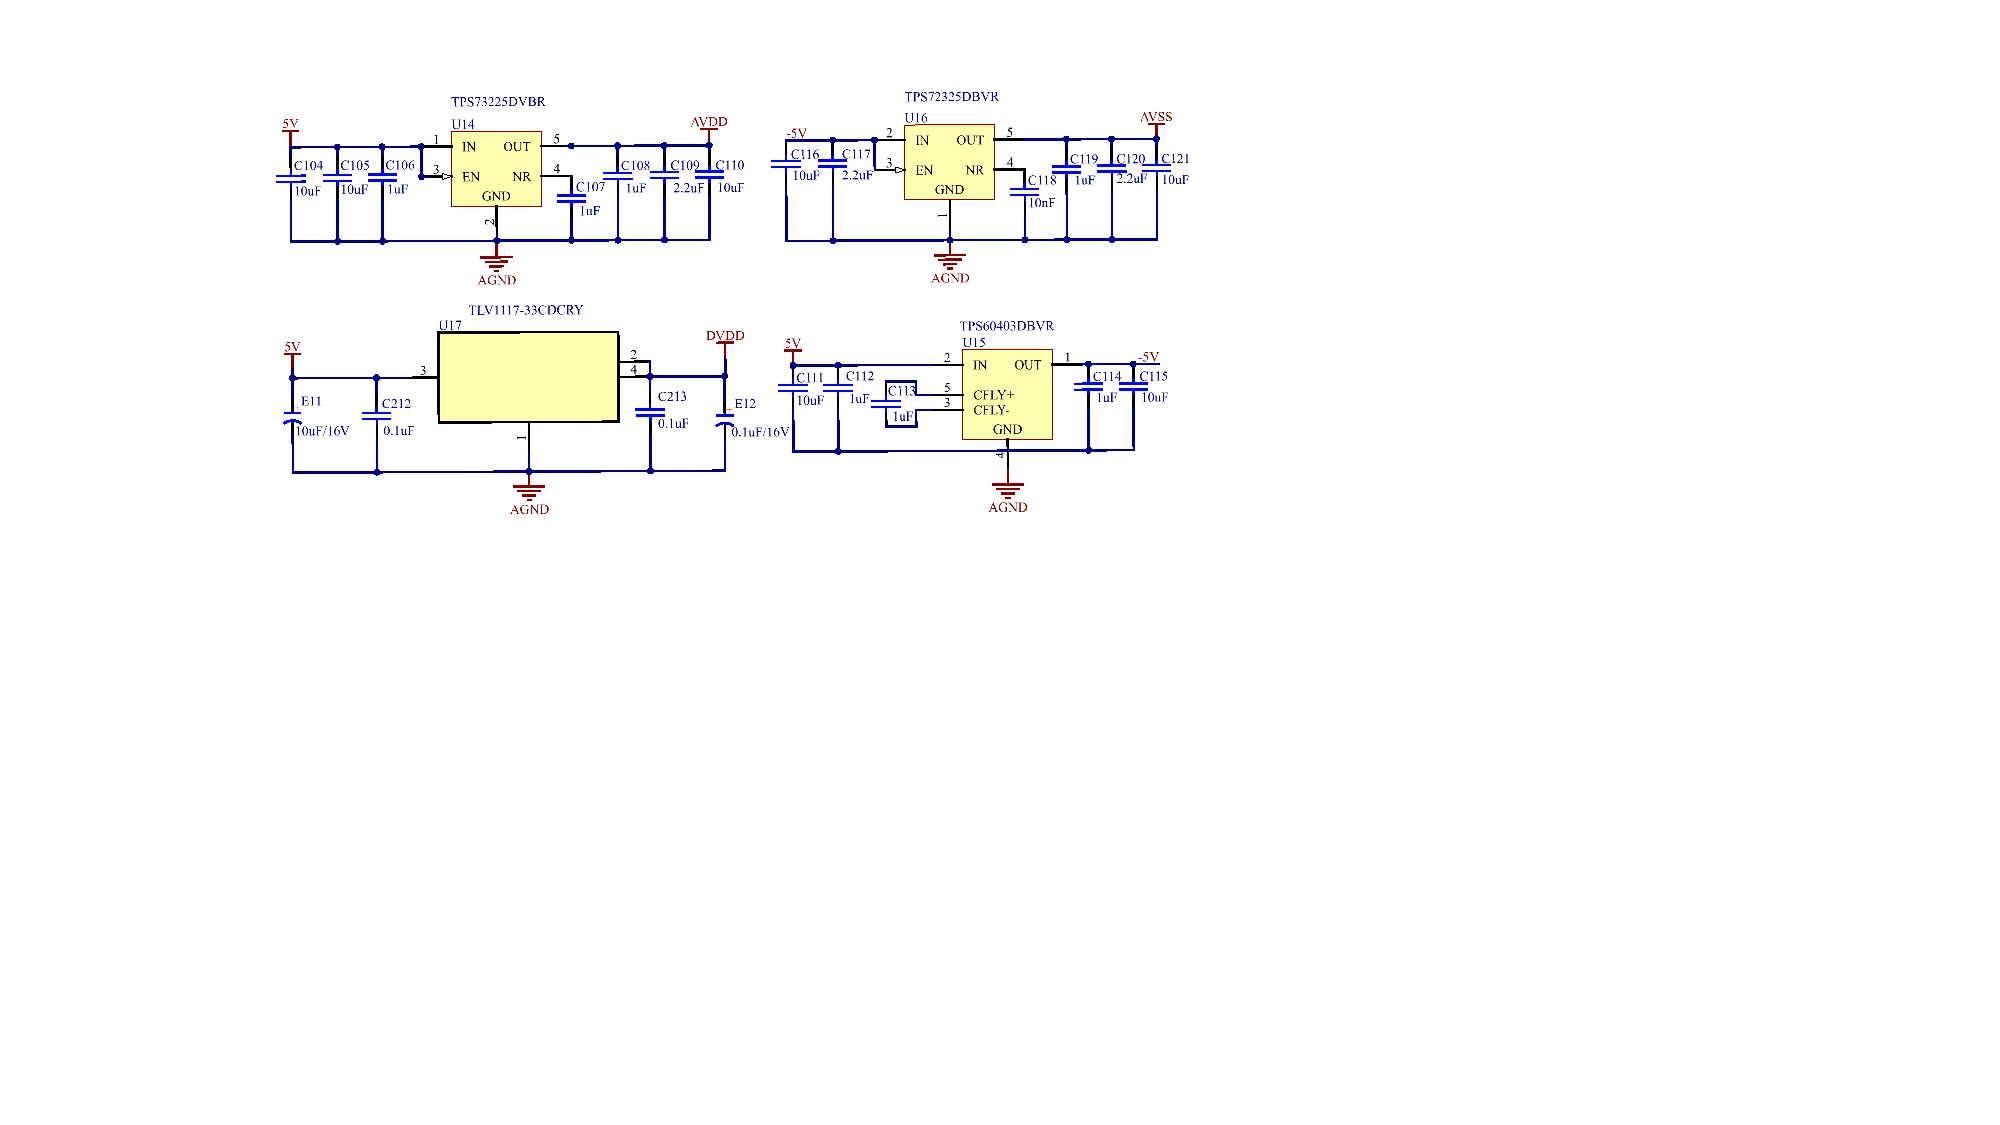
\includegraphics[width=0.62\textheight]{模拟电源模块.pdf}
	\caption{模拟电源模块原理图}
	\label{fig2-7}
\end{figure}

\subsection{STM32H743IIT6主控模块设计}
\begin{figure}[!h]
	\centering
	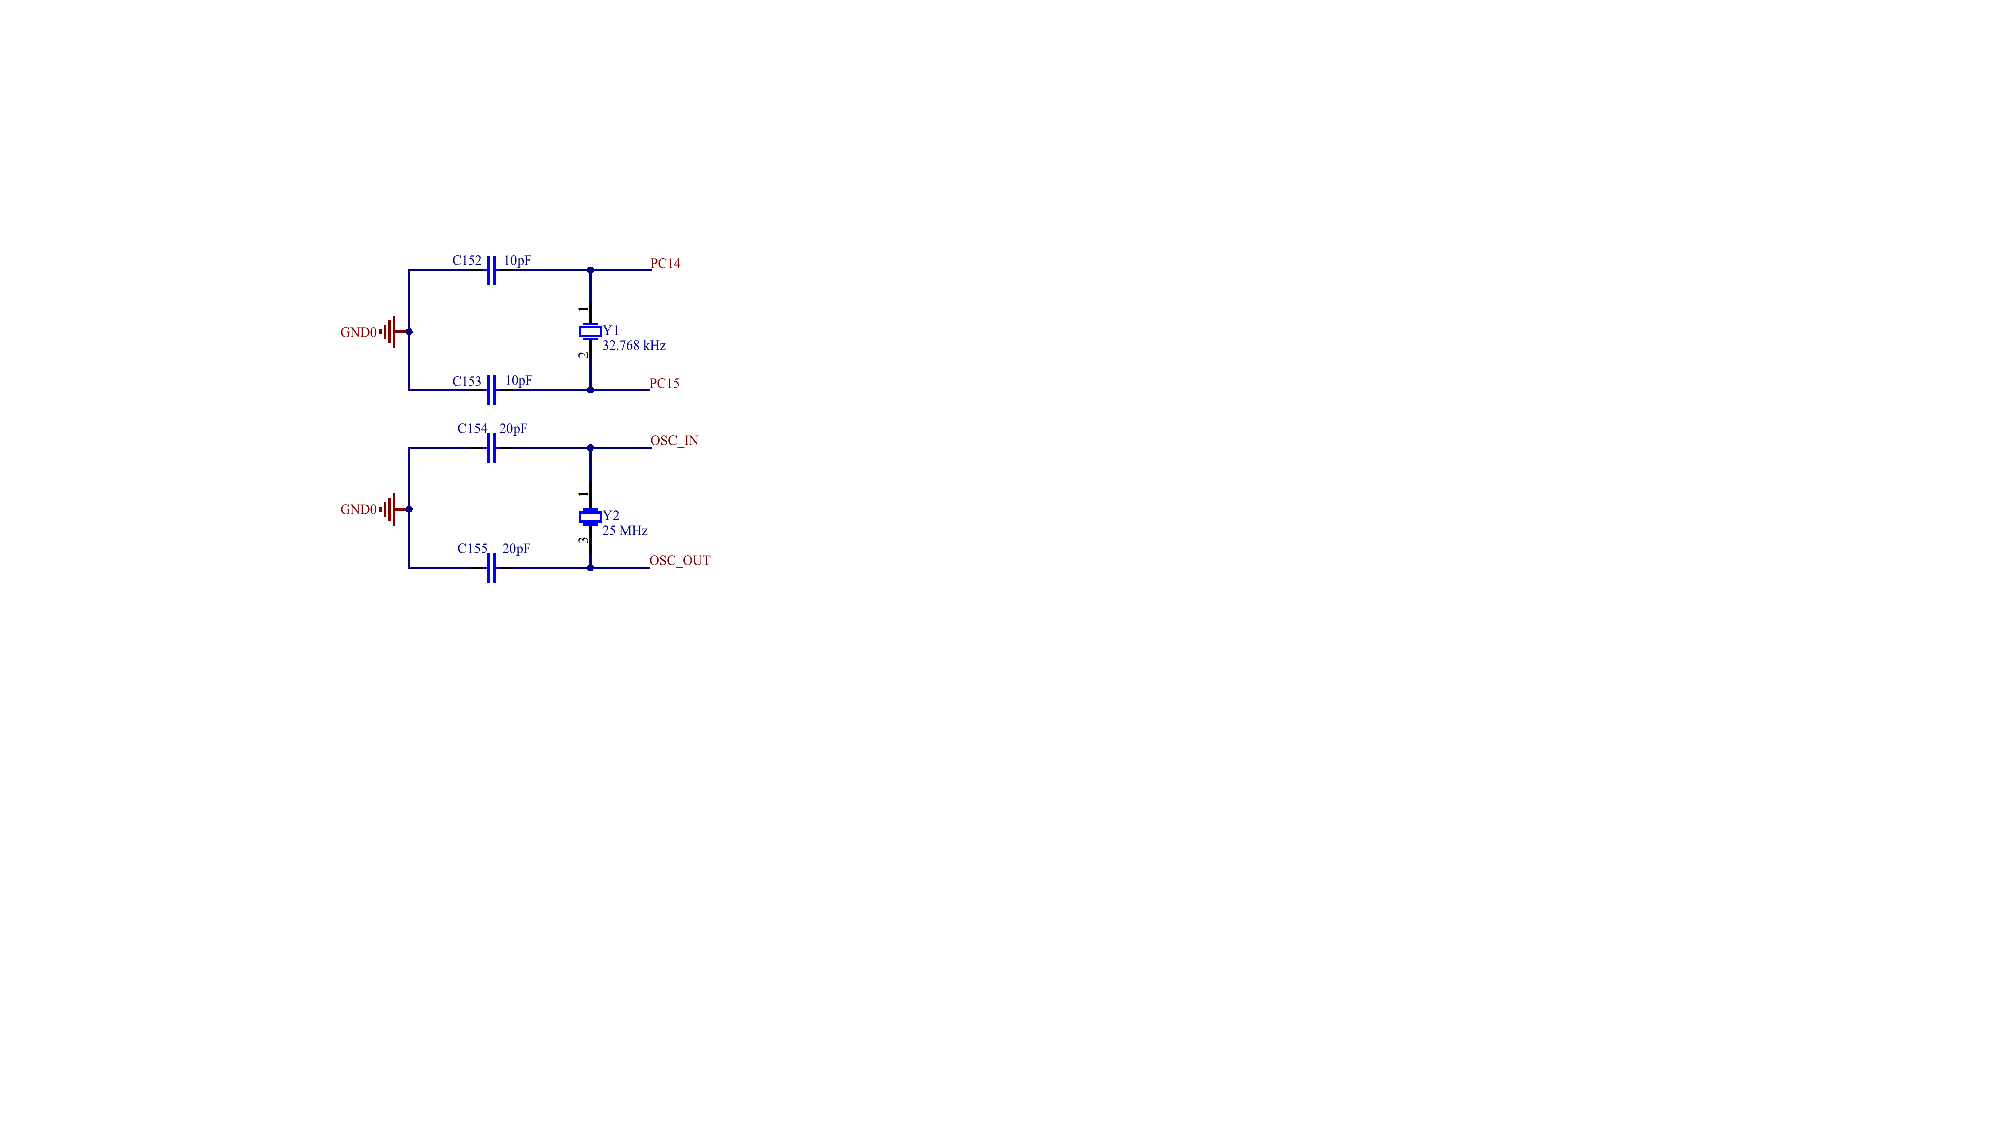
\includegraphics[width=0.32\textheight]{时钟电路.pdf}
	\caption{时钟电路原理图}
	\label{fig2-8}
\end{figure}

JS-AINS-40系统的主控模块围绕STM32H743IIT6芯片搭建。主控模块负责:配置ADS1299设置寄存器,使其以期望模式采样EEG数据;接收、切割、存储ADS1299回传的数据;将处理后的回传数据通过虚拟串口通信模块转发给上位机。

为了保证主控模块正常工作,给STM32H743IIT6芯片搭建了配套的时钟电路、复位电路和调试电路。其原理图如图\ref{fig2-8}所示。根据STM32H743IIT6的芯片手册,使用爱普生公司的X1E0000210621 25 MHz晶振和Q13FC1350000400 32.768 kHz晶振设计时钟电路,分别作为高速时钟源和低速时钟源。外部高速时钟源通过PLL锁相环电路倍频至400 MHz,维持系统内核时钟稳定。外部低速时钟源保证看门狗和实时时钟(Real Time Clock,RTC)不受其他因素干扰。


复位电路能够保证每次上电开机后,主控模块自动复位,同时能够在必要时通过手动复位芯片。其原理图如图\ref{fig2-9}所示,开机时或按键后,STM32的RESET引脚将被拉低。

\begin{figure}[!h]
	\centering
	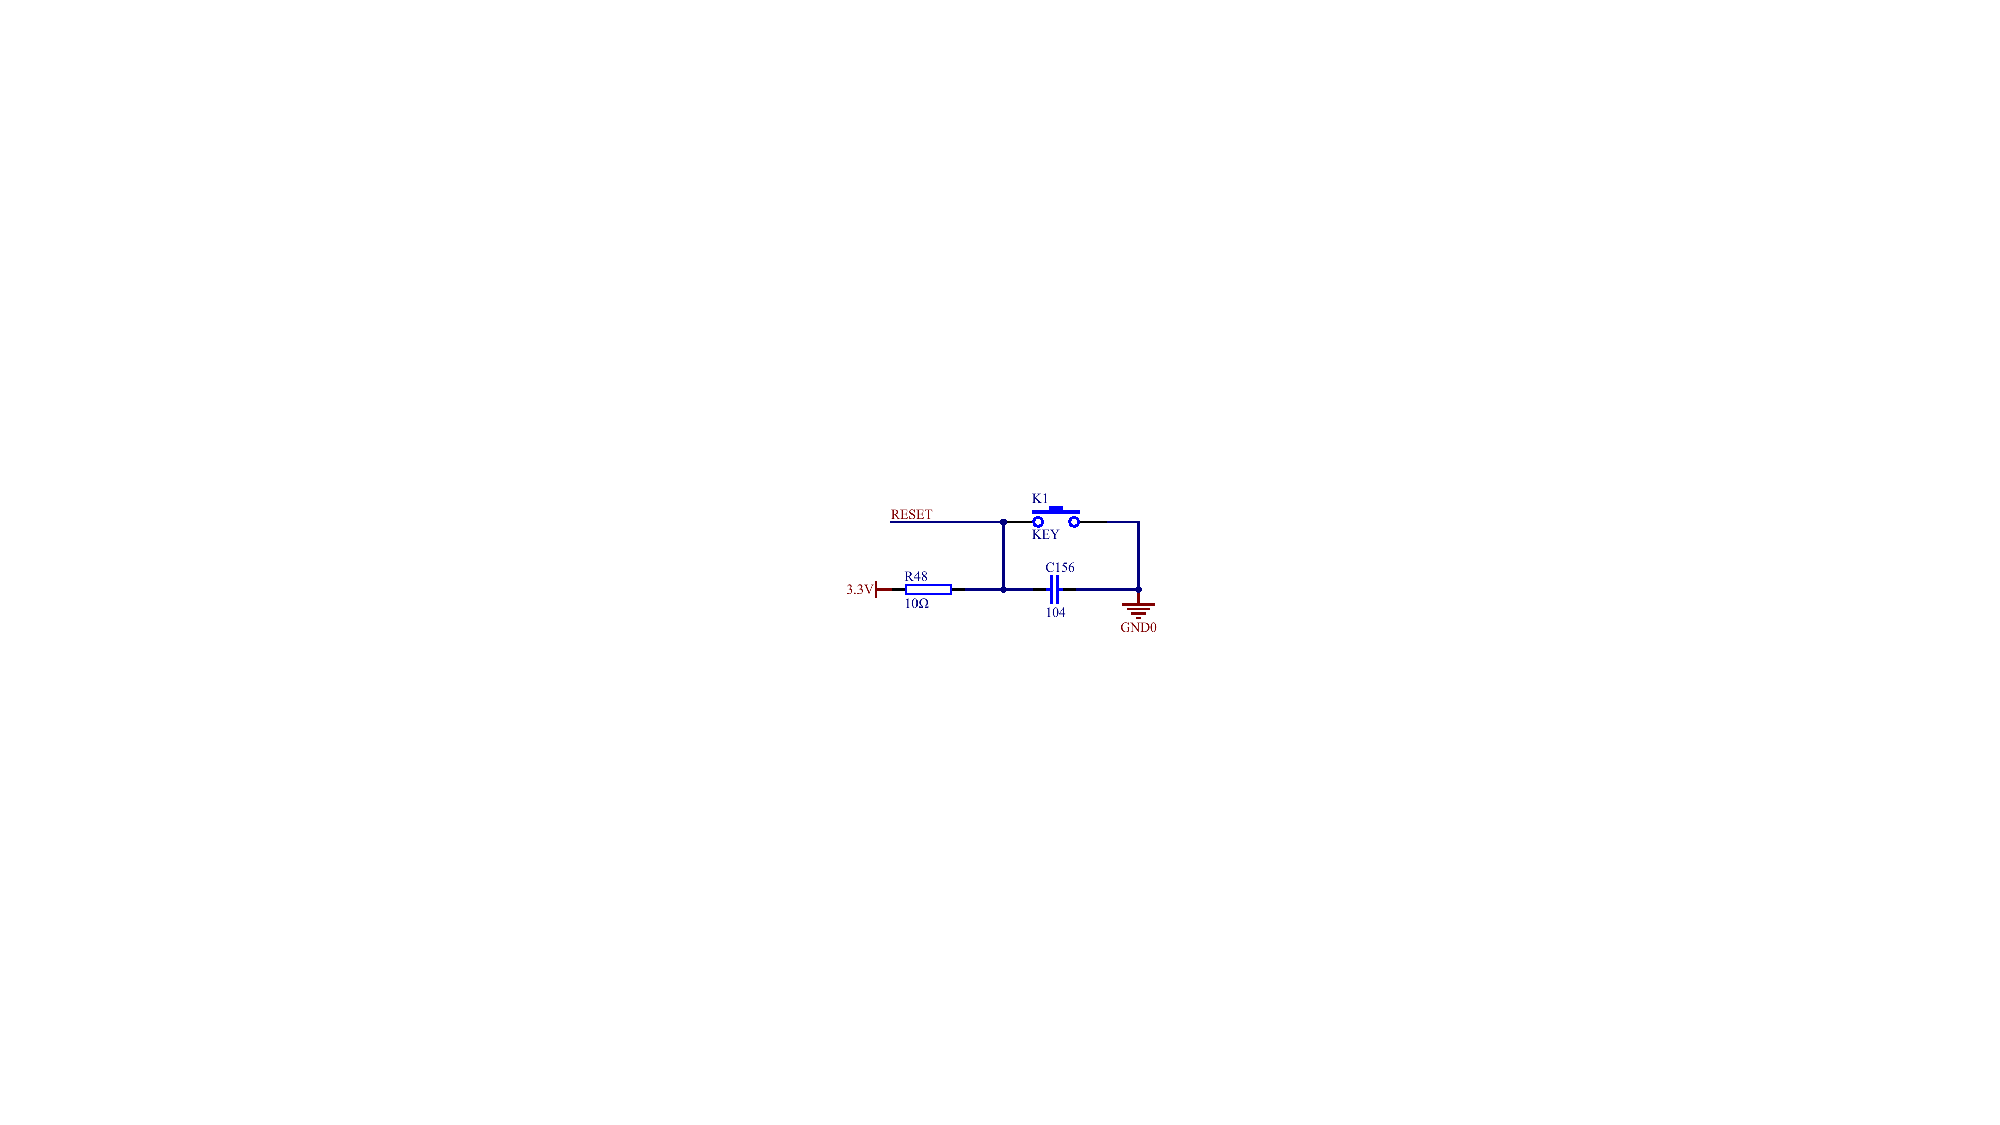
\includegraphics[width=0.24\textheight]{复位电路.pdf}
	\caption{复位电路原理图}
	\label{fig2-9}
\end{figure}

调试电路遵循ARM公司提出的SWD(Serial Wire Debug)协议进行设计。SWD协议能够利用串行通信直接访问ARM Cortex内核的寄存器,在高速模式下比传统的JTAG协议更为可靠。同时,相较于JTAG协议,SWD的引脚数更少,其仅需SWDIO、SWCLK、SWO和RESET四根数据线即可正常工作。这为PCB设计节省了更多的空间,并有效减少了对STM32芯片IO资源的占用。SWDIO:SWD的双向数据信号线,用来提供串行数据的输入输出;SWCLK:SWD的时钟信号线,提供串行时钟输入;SWO:可选择的串行数据输出引脚;RESET:系统复位信号线。本章设计的主控模块通过SWD协议进行程序烧录和Debug调试。

同时,为了能够方便地判断当前设备工作状态,还设计了相关的LED电路。

\subsection{ADS1299采集模块设计}

ADS1299作为采集模块的核心,其将EEG信号的采集、放大、模数转换和数据传输进行了集成。这一设计成功避免了将上述功能分别实现所可能带来的兼容问题以及外界环境干扰,使ADS1299拥有达到110 dB的共模抑制比、低于1 $\mu V_{pp}$的输入噪声和超过500 M$\Omega$的输入阻抗。同时,这一设计也大幅降低了EEG采集系统的开发难度。图\ref{fig2-10}与图\ref{fig2-11}展示了ADS1299的引脚。其具体功能为:

\begin{figure}[h]
	\centering
	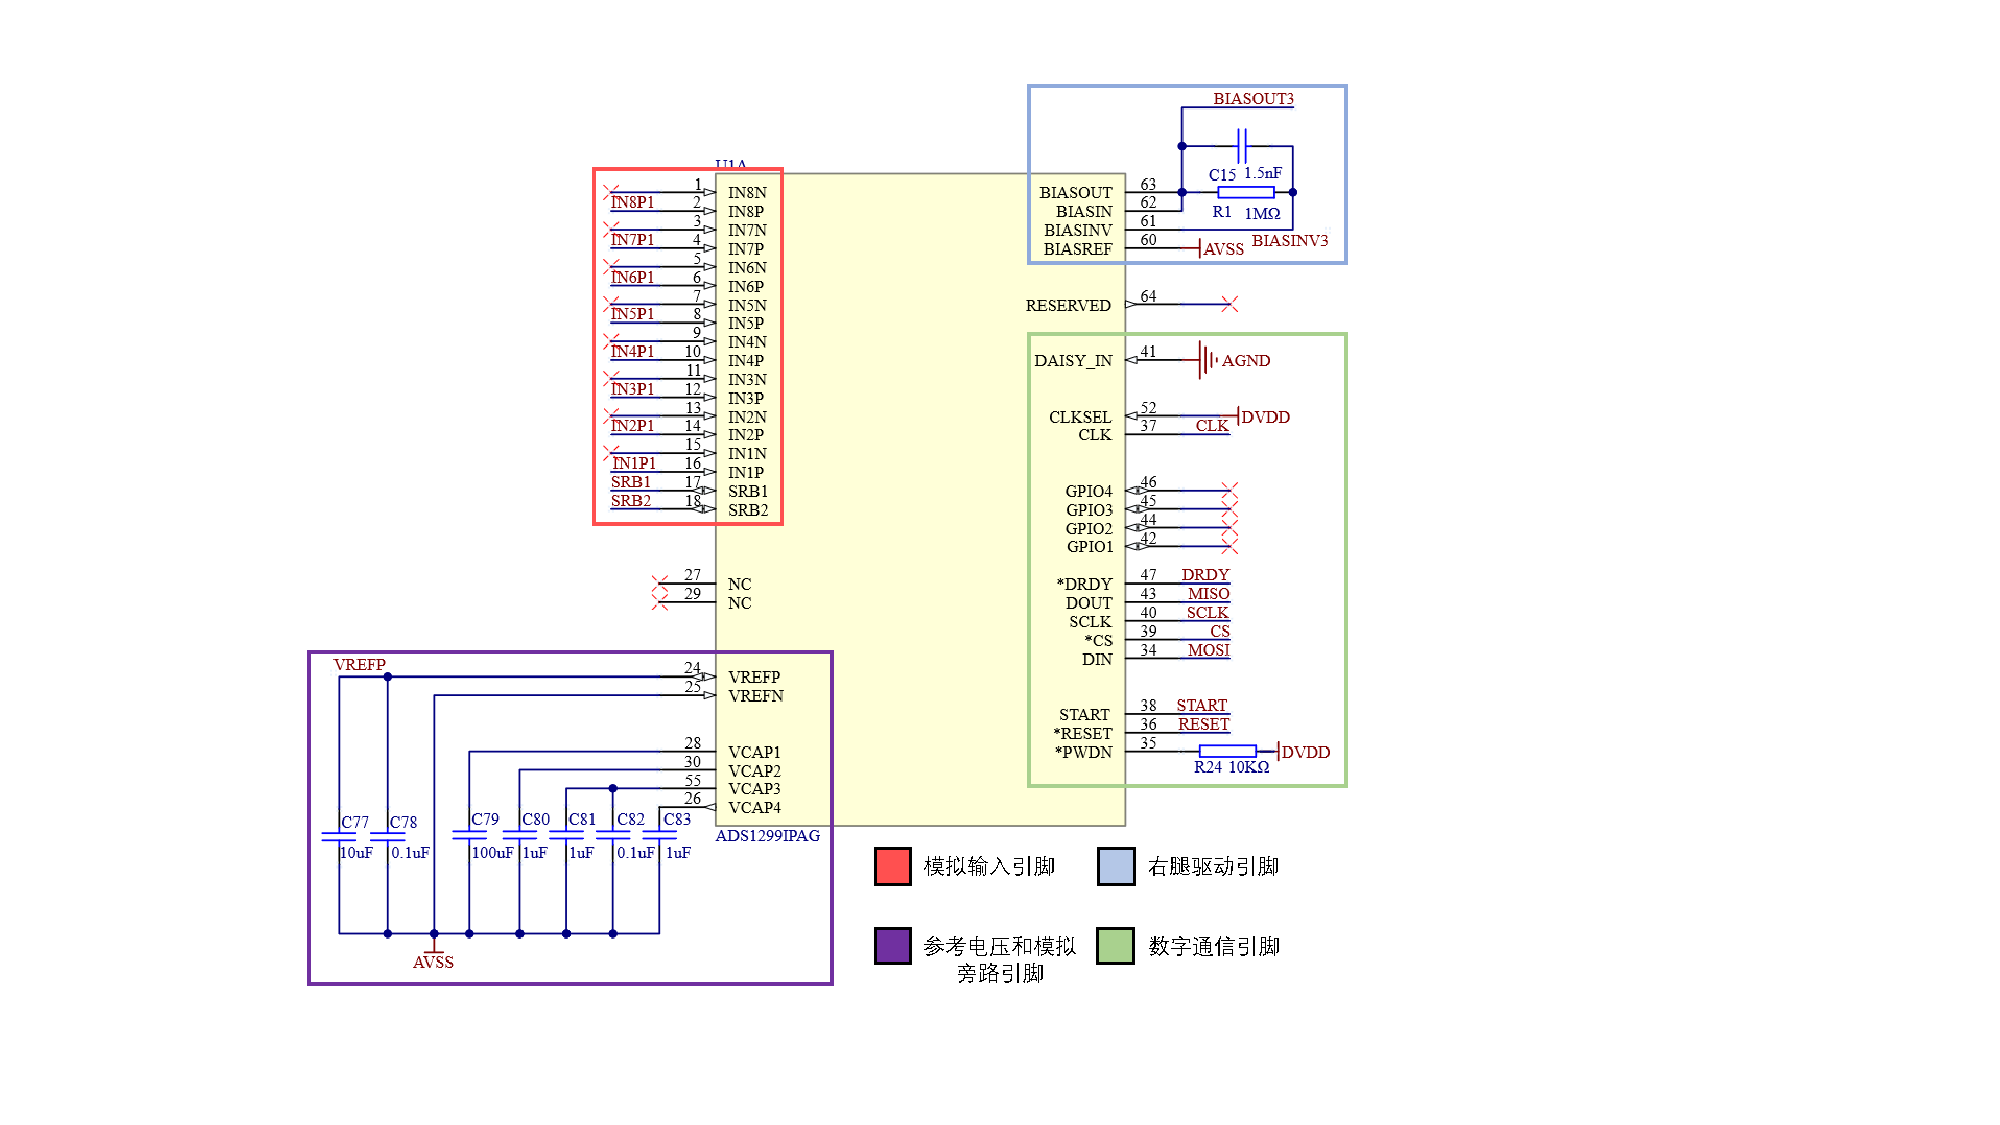
\includegraphics[width=0.605\textheight]{ADS1299功能引脚.pdf}
	\caption{ADS1299功能引脚}
	\label{fig2-10}
\end{figure}


(1) 模拟输入引脚:每块ADS1299芯片具有8通道的模拟差分输入(每个通道包含一个P端和一个N端),即图\ref{fig2-10}中的1-16引脚。同时,还包括了公共端SRB1和SRB2。SRB1/SRB2通过ADS1299内部寄存器进行配置后,可作为所有N/P端的公共引脚。

(2) 参考电压和模拟旁路引脚:参考电压引脚的VREFN端将AVSS接入,用来生成ADS1299内部的4.5 V参考电压。模拟旁路引脚通过电容将电源的高频噪声引向AVSS,防止其干扰采集过程。

(3) 数字通讯引脚:DAISY\_IN引脚用来设置是否采用菊花链式连接;CLKSET用来选择时钟源,高电平时使用内部时钟;CLK引脚用来输出内部时钟信号(内部时钟源)或者接受外来时钟信号(外部时钟源);GPIO是ADS1299正常工作模式下的数字I/O引脚;DRDY是模数转换的标志引脚,拉低时标志转换完成;DOUT,SCLK,CS,DIN是SPI通讯引脚;START引脚和RESET引脚分别控制芯片的启动和复位,其中START高电平生效,RESET低电平生效;PWDN引脚用来控制芯片上电。

(4) 右腿驱动引脚:60-63引脚用来实现芯片的右腿驱动功能,输出反向的共模噪声信号,降低共模干扰。

(5) 电源引脚:如图\ref{fig2-11}所示,遵照ADS1299数据手册要求,完成外围供电电路设计。


\begin{figure}[h]
	\centering
	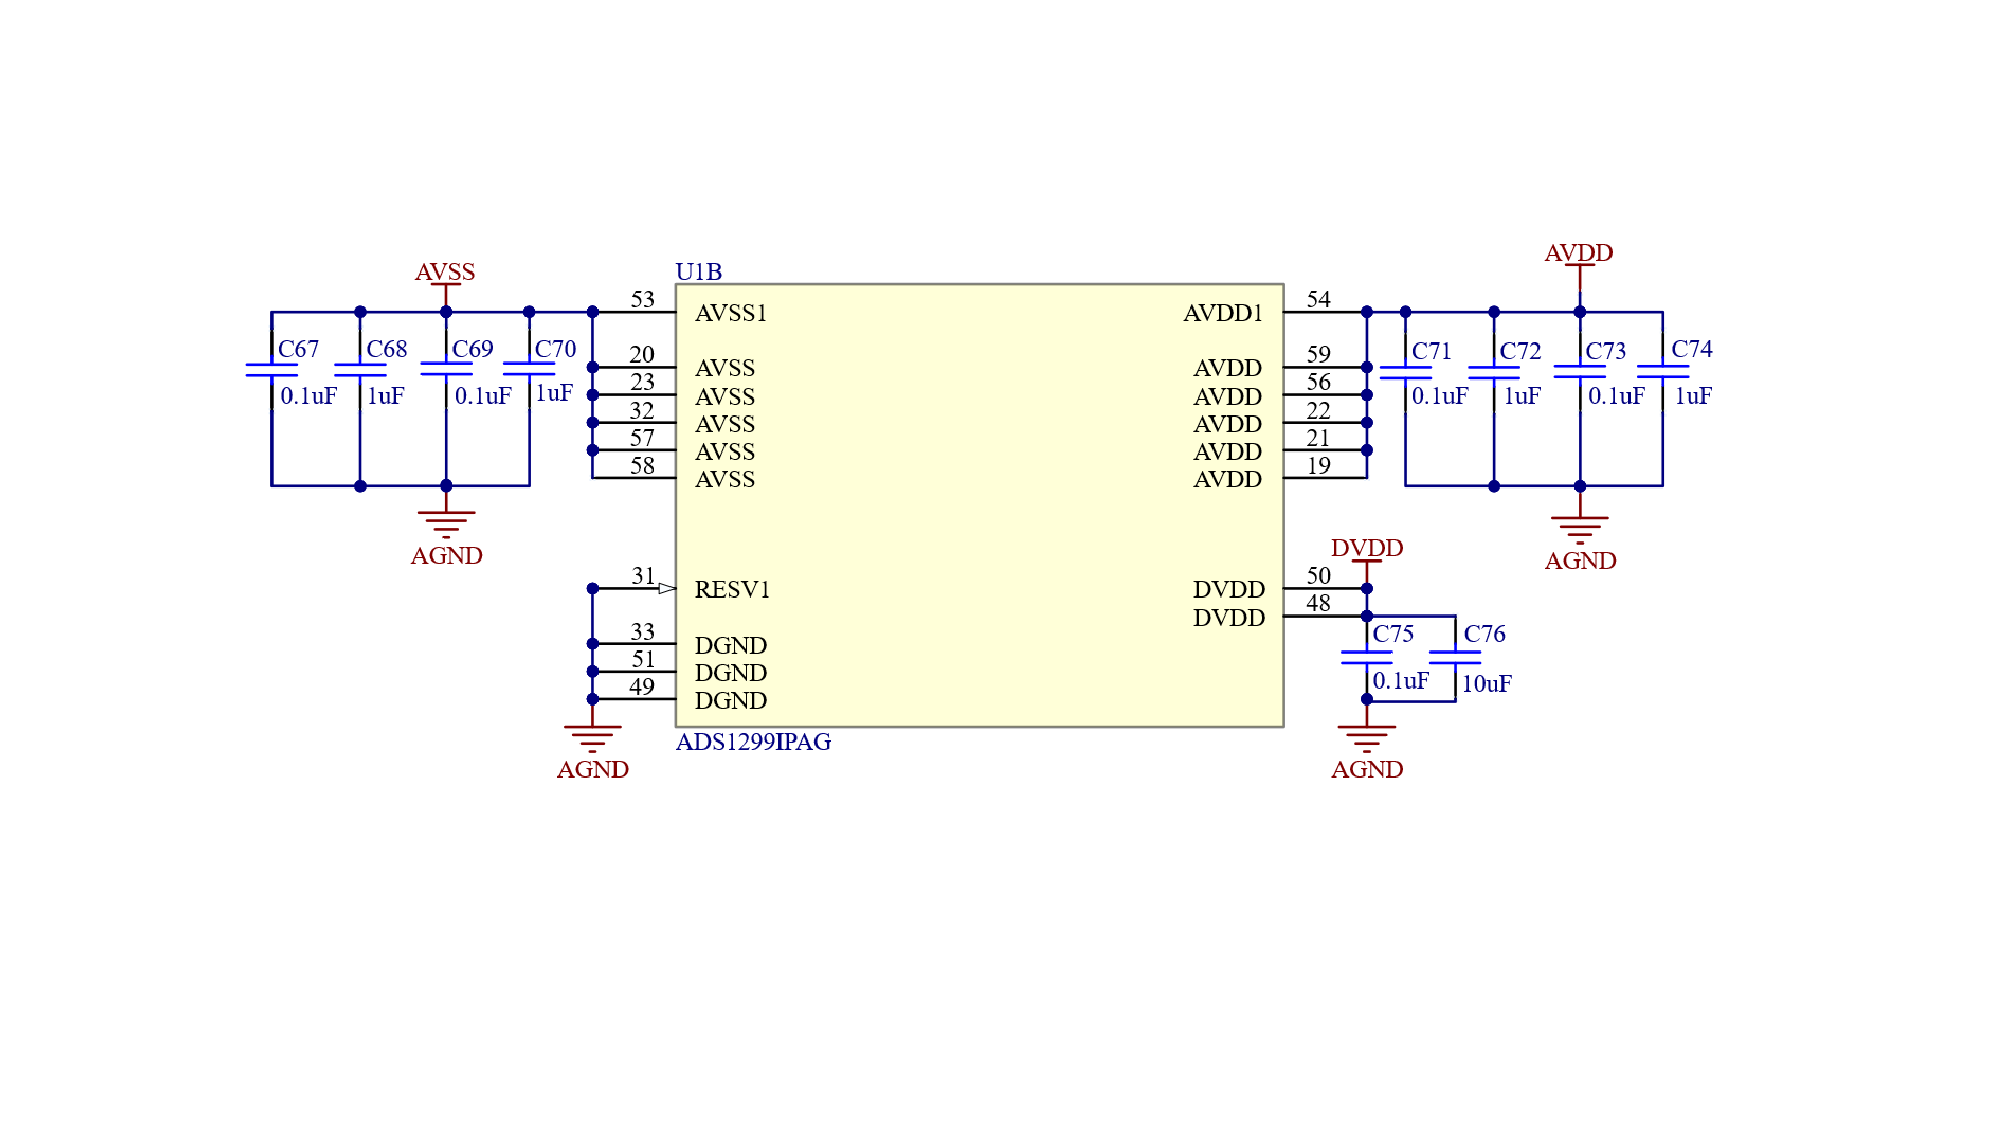
\includegraphics[width=0.61\textheight]{ADS1299电源引脚.pdf}
	\caption{ADS1299电源引脚} 
	\label{fig2-11}
\end{figure}

由于一块ADS1299芯片仅包含8个数据采集通道,因此实现40导联的EEG采集需要5块ADS1299协同工作。ADS1299官方给出了两种不同的多芯片协同方式:标准配置(Standard Configuration)和菊花链配置(Daisy-Chain Configuration)。其中标准配置能够方便地读取所有芯片的寄存器设置,有利于进行设备调试与维护,因此选取标准配置。
\begin{figure}[!h]
	\centering
	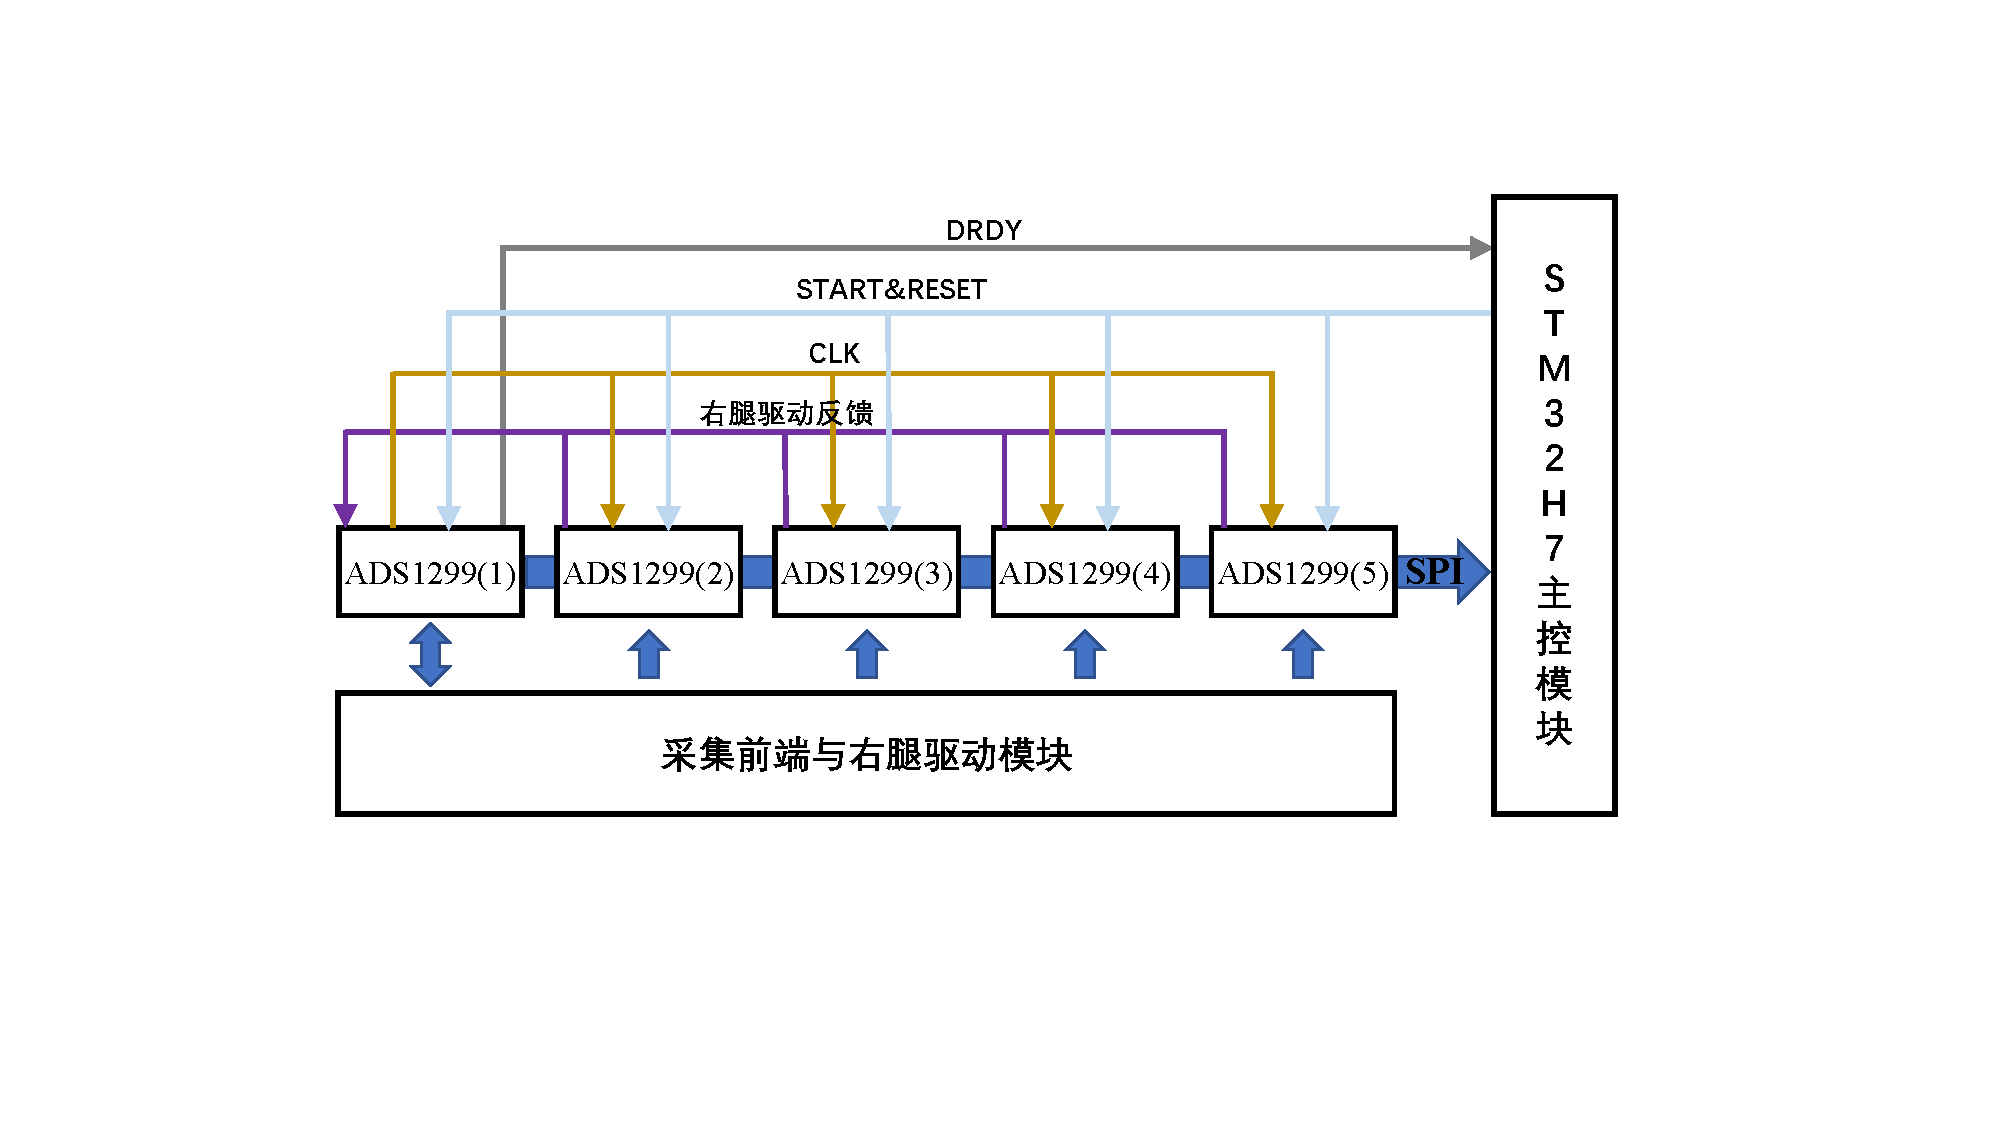
\includegraphics[width=0.5\textheight]{ADS1299连接拓扑图.pdf}
	\caption{ADS1299连接拓扑图} 
	\label{fig2-12}
\end{figure}

本章设计基于标准配置进行,因此首先将DAISY\_IN引脚拉低。接下来,将详细叙述多芯片协同的设计思路。第一步,选取一块ADS1299作为主芯片,开启其内部时钟,并通过寄存器配置其向外输出时钟信号。其他从属芯片使用主芯片的时钟信号,与主芯片保持同步。第二步,在主控模块利用START引脚启动所有芯片后,五块芯片将同时完成数据采集与模数转换,因此只需将主芯片的DRDY接入主控模块即可掌握所有芯片的工作状态。第三步,在DRDY拉低后,通过SPI依次读取所有芯片的数据,实现数据采集。最后,所有从属芯片采集的共模噪声信号将传递给主芯片,统一反馈给人体,消除共模噪声干扰。图\ref{fig2-12}显示了5片ADS1299的连接拓扑图。

\subsection{SPI隔离模块设计}

数字模块和模拟模块之间不仅有电源部分相连,还通过SPI进行数据传输。这可能造成外部噪声进入模拟端,影响EEG数据采集。因此本节在设计时不仅引入了电源隔离模块,还加入了SPI隔离模块。选取川土微公司(Chipanalog)生产的CA-IS3741LN高速四通道数字隔离器作为SPI隔离,其信号传输速率达到150 Mbps、无需启动初始化、传播延迟仅为8 ns并且拥有高达5 $kV_{RMS}$的隔离电压。良好的绝缘能力也使其能够防止其他线路上的噪声和浪涌进入本地接地端,对EEG数据采集造成干扰。经过计算,其参数指标符合当前的设计要求。CA-IS3741LN的原理图如图\ref{fig2-13}。为防止在上电瞬间产生误动,对所有CA-IS3741LN的前向通道增加下拉电阻,保证隔离后信号的确定性。
\begin{figure}[!h]
	\centering
	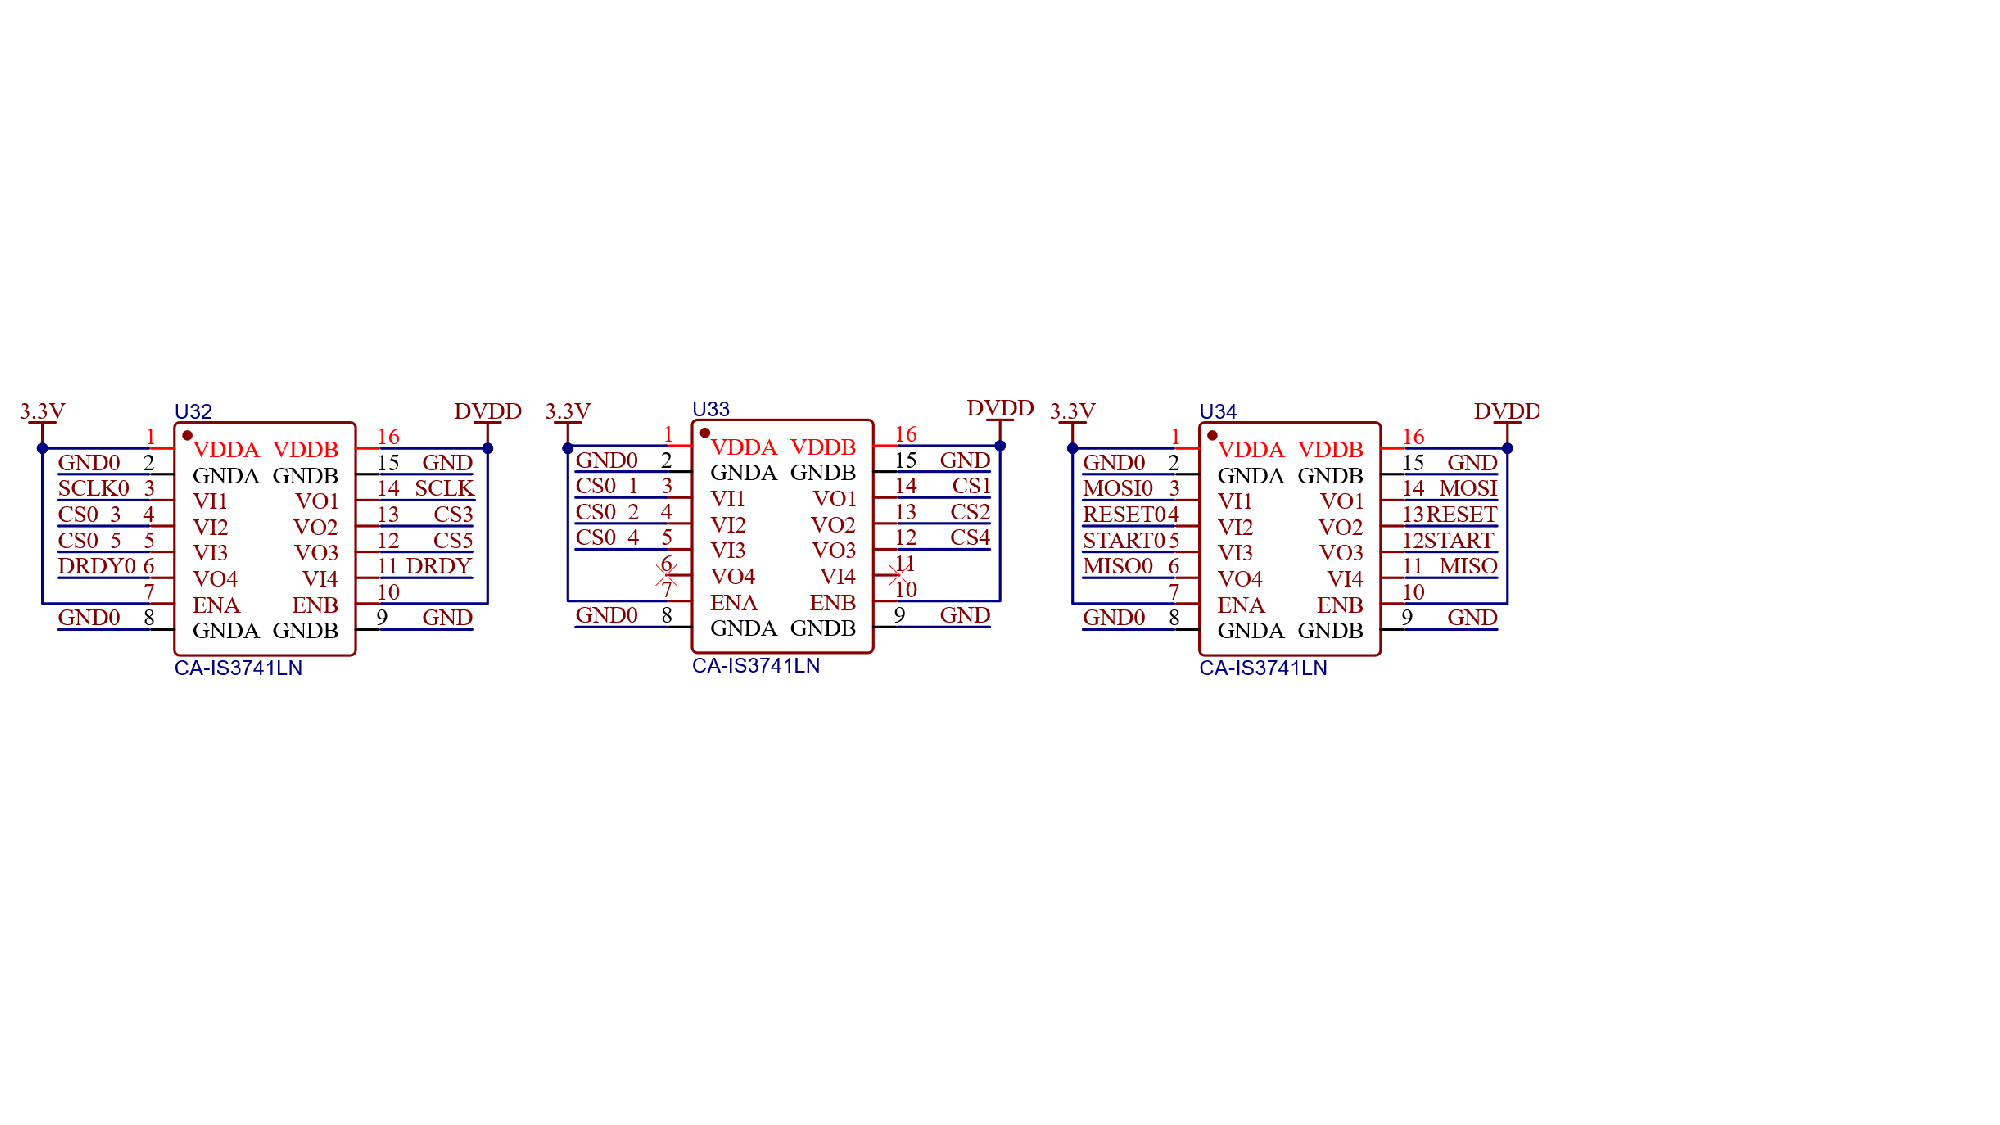
\includegraphics[width=0.61\textheight]{SPI.pdf}
	\caption{SPI隔离模块原理图} 
	\label{fig2-13}
\end{figure}

\subsection{虚拟串口通讯模块}
虚拟串口通讯模块在STM32自带的USB功能上进行实现。STM32H743IIT6内置USB\_OTG\_FS(全速双角色设备控制器)和USB\_OTG\_HS(高速双角色设备控制器),支持作为USB从设备使用的同时还能够作为USB主机使用。USB\_OTG\_FS的理论通讯速度为12 Mbps,符合本章设计需求。同时,相较于USB\_OTG\_HS,其无需外置高速PHY芯片,仅需使用USB\_DM和USB\_DP两个引脚即可实现通信,因此本节采用USB\_OTG\_FS完成设计。

\subsection{采集前端与右腿驱动模块设计}

根据EEG信号的频域特性,在采集前端设计相应的一阶低通滤波电路来对EEG信号进行预处理,消除可能存在的高频噪声。由于EEG信号基本集中在200 Hz以下的频带范围内,因此本节将一阶低通滤波电路的截止频率设计为500 Hz。考虑到RC滤波电路的截止频率计算公式为:

\begin{equation}
    \label{deqn_ex2_2}
    f_c = \frac{1}{2\pi RC}
\end{equation}

考虑到电阻阻值较大时更容易引入噪声,因此选取较小的阻值$\rm R= 800$ $\Omega$,此时$\rm C = 200$ $nF$。这一设计在500 Hz时信号衰减达到$\rm -3$ $dB$,信号功率衰减为原来的50\%。在5 kHz以上时,衰减达到$\rm -20$ $dB$。


人体在采集过程中,无法完全屏蔽周围电磁环境带来的影响。当受到周围电网形成的交流电场作用时,人体表面会产生工频交流电位。作为一种共模干扰,其可能会掩盖生物电信号,对EEG采集造成影响。针对这一问题,右腿驱动电路应运而生。作为一种成功的应对共模干扰的技术,右腿驱动电路被广泛应用于生理电信号测量当中\cite{2-4}。图\ref{fig2-14}展示了右腿驱动电路的具体组成。

\begin{figure}[!h]
	\centering
	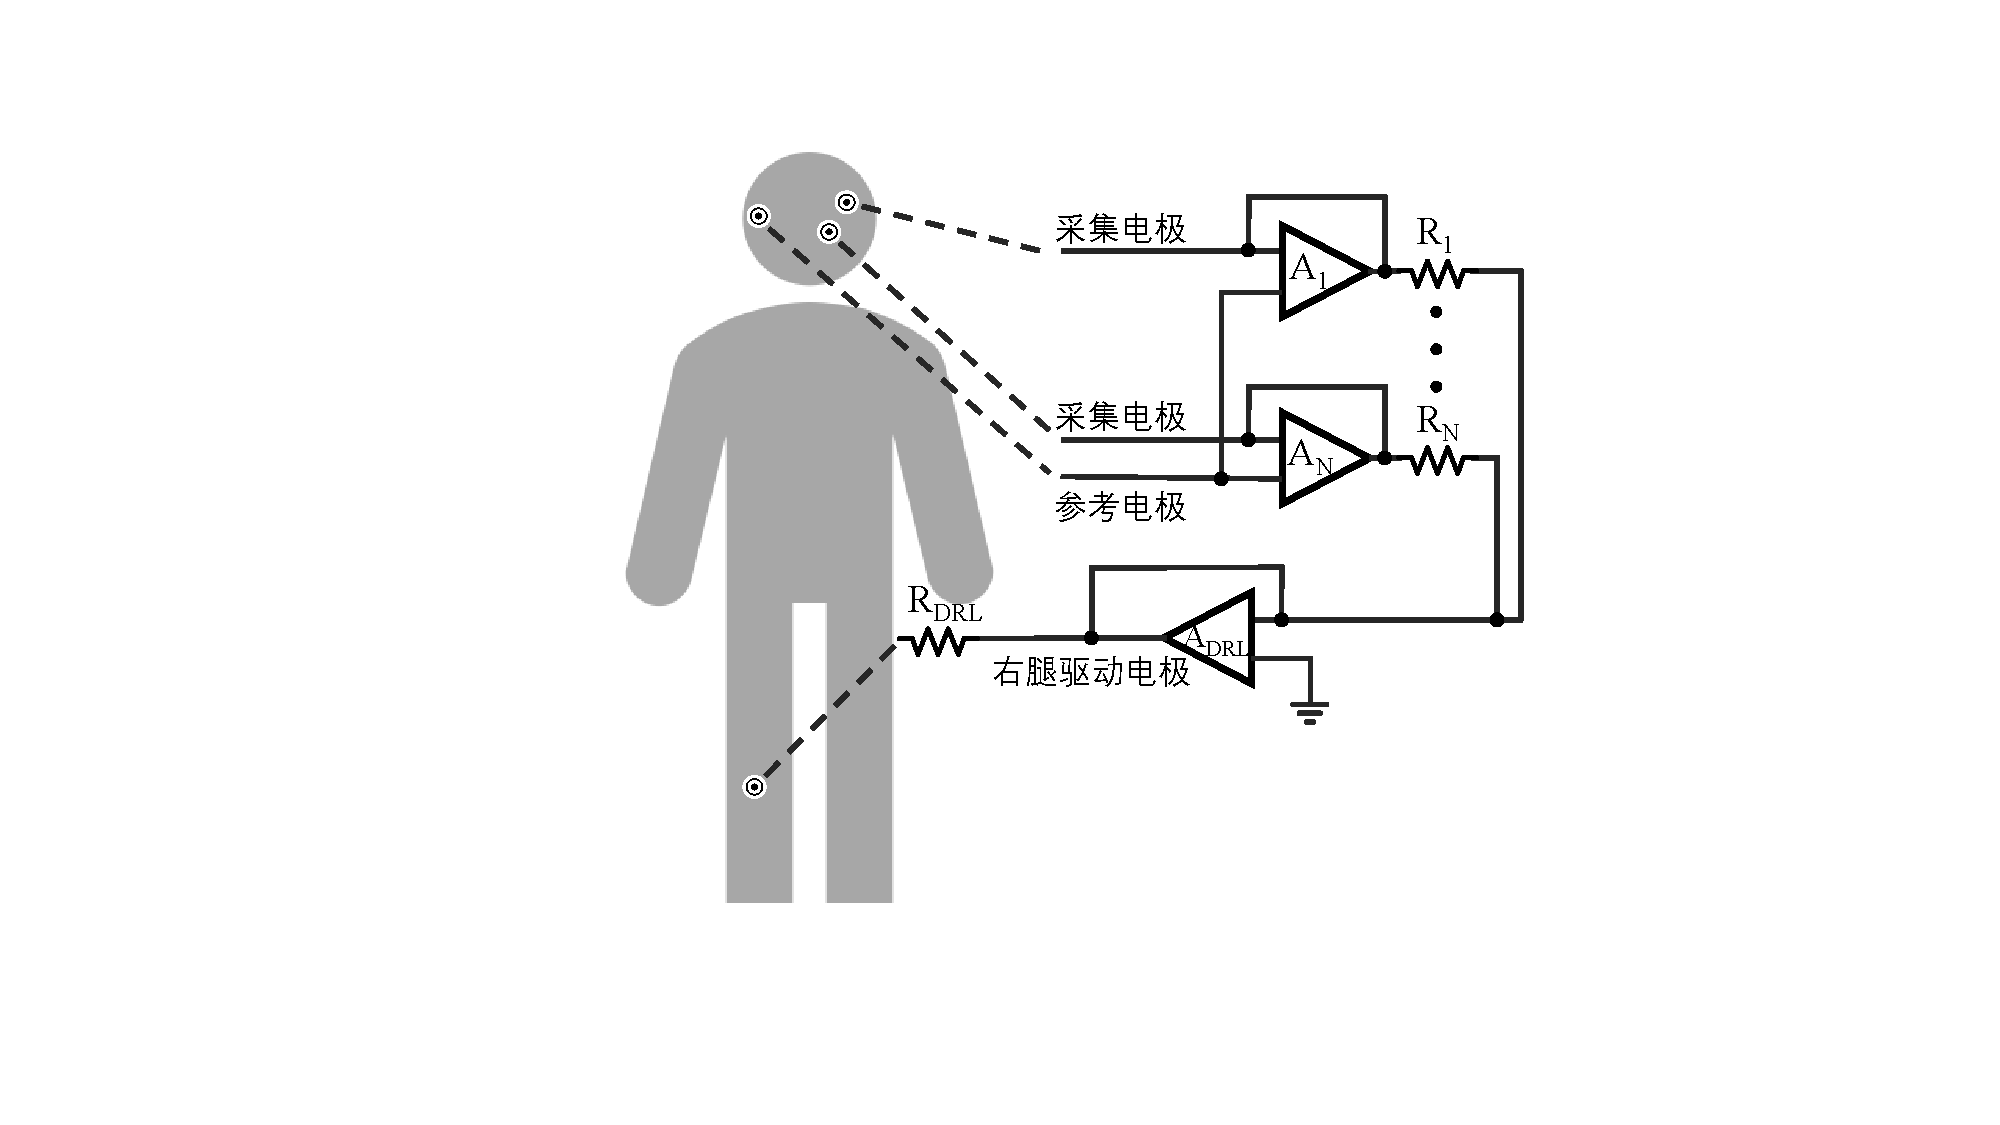
\includegraphics[width=0.35\textheight]{右腿驱动.pdf}
	\caption{右腿驱动电路} 
	\label{fig2-14}
\end{figure}

右腿驱动电路的原理如下所述:首先,EEG电极采集得到的原始EEG信号,经由一组低噪声PGA $\rm A_1-A_N$组成的差分放大电路传递至$\rm R_1-R_N$,此时的原始信号中包含了大量的共模分量。接下来,通过$\rm R_1-R_N$的共模信号在累加后被$\rm A_{DRL}$反向放大,经由$\rm R_{DRL}$重新传递回受试者皮肤表面以消除共模干扰。本节在设计时,综合考量受试者的使用习惯并参考ADS1299的数据手册,将参考电极放置在左耳后乳突处,将右腿驱动电极放置在右耳后乳突处。

\begin{figure}[h!]
	\centering
	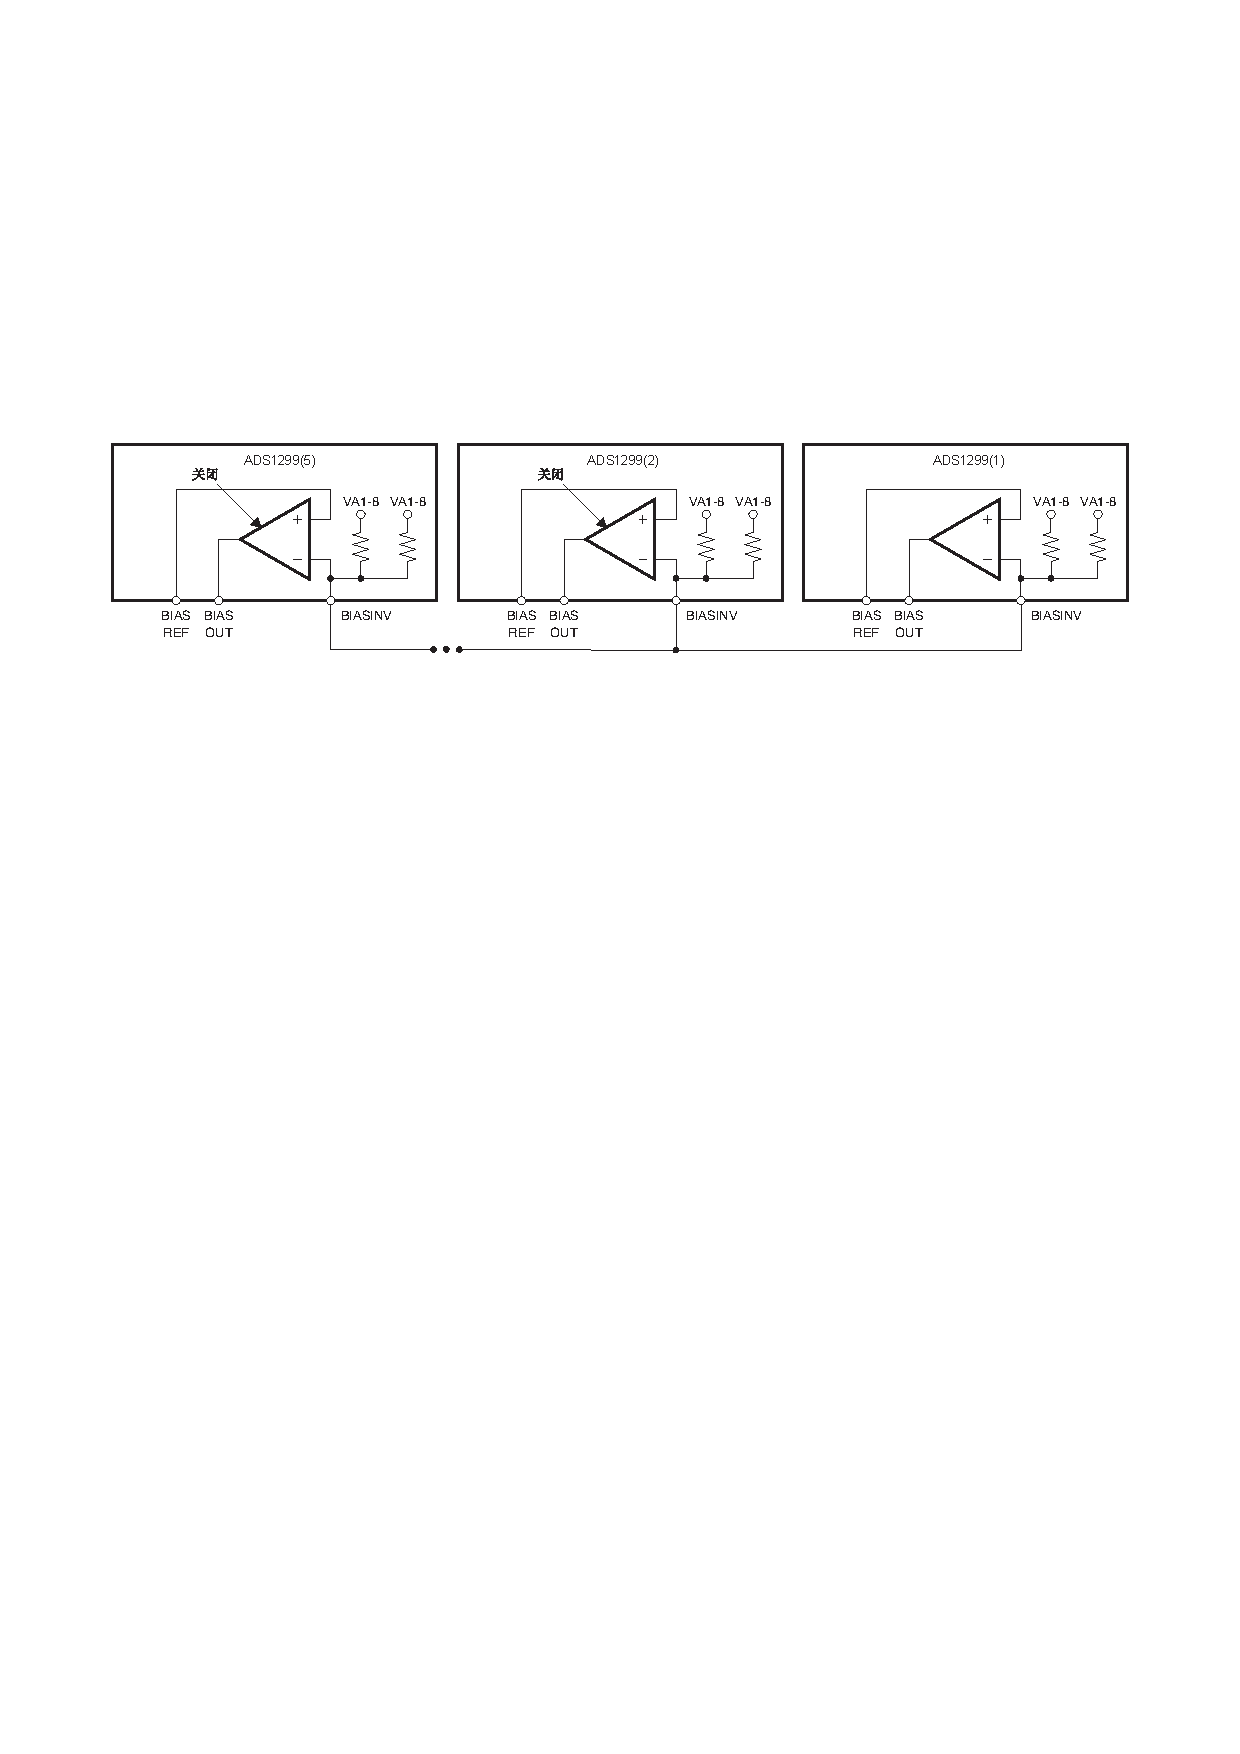
\includegraphics[width=0.605\textheight]{右腿驱动级联.pdf}
	\caption{ADS1299多芯片右腿驱动配置} 
	\label{fig2-15}
\end{figure}

ADS1299中已经集成了右腿驱动电路,本节在设计时只需考量如何对多组电路进行协同。多芯片级联方式如图\ref{fig2-15},开启主ADS1299芯片的$\rm A_{DRL}$,关闭其他从芯片的$\rm A_{DRL}$,将所有的共模信号累加至主芯片后统一反馈给人体。

\subsection{静电与过载保护设计}
考虑到EEG采集的实际使用环境,为了防止静电从与外界接触的采集端,USB输入端以及开关按钮处进入PCB内部,干扰数据采集甚至影响设备运行,本节在相应位置引入了静电放电(Electro-Static Discharge,ESD)保护芯片。在充分考虑设备的电磁兼容性问题后,三款不同的ESD保护芯片被分别设计在PCB的采集端,USB输入端以及开关按钮的电路中。详细设计如下:

\begin{figure}[!h]
	\centering
	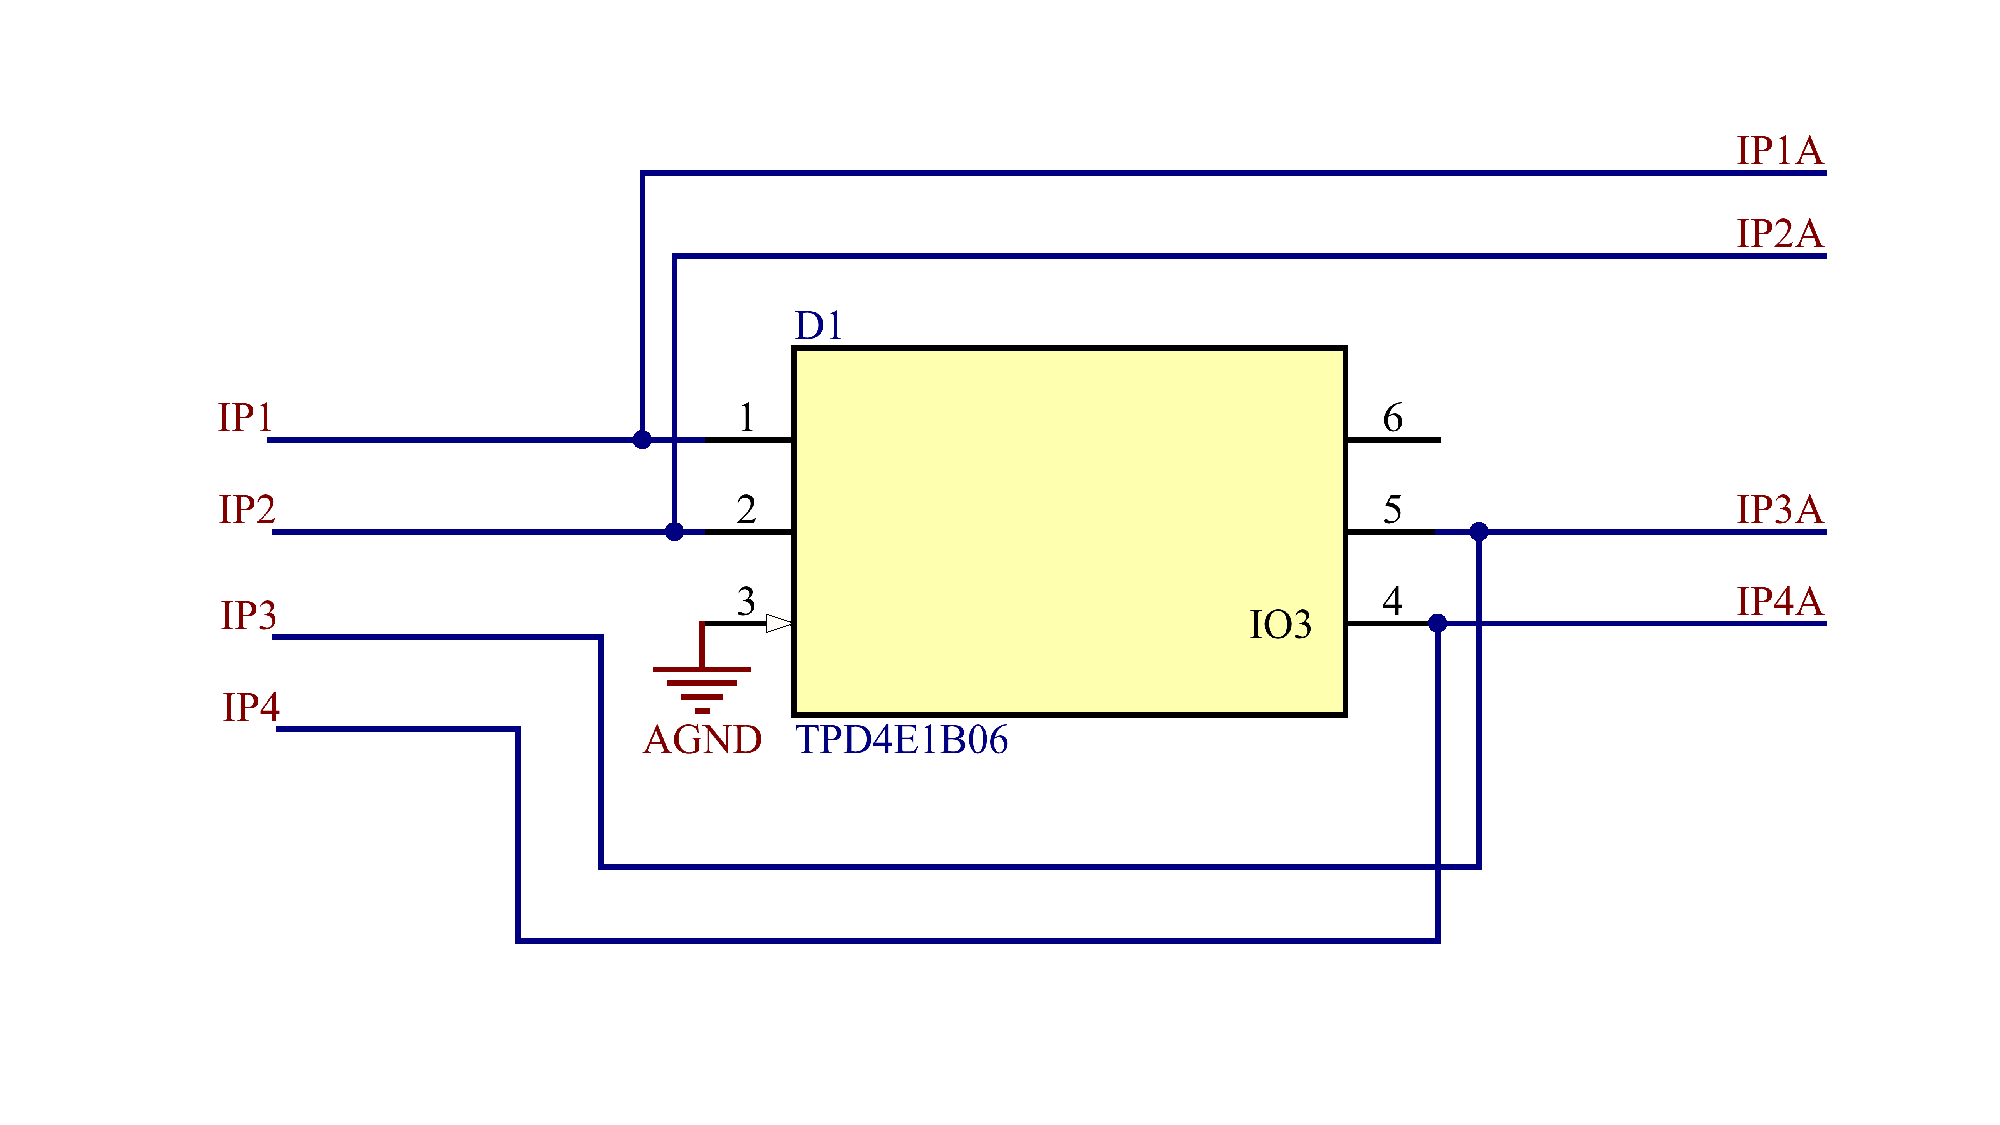
\includegraphics[width=0.42\textheight]{采集端ESD.pdf}
	\caption{TPD4E1B06原理图} 
	\label{fig2-16}
\end{figure}

(1) 采集前端处,使用TPD4E1B06 4通道ESD保护器件保护采集端口。TPD4E1B06是德州仪器公司设计的一款4通道双向瞬态电压抑制器(Transient Voltage Suppressor,TVS)二极管阵列。这款芯片能够为设备提供$\pm12$ kV的接触和$\pm15$ kV空气间隙放电保护。其漏电流仅为0.5 nA,能够为模拟信号的精确测量提供保障。$\rm 0.7$ pF的线路电容值使其能够应用于医疗设备之中。同时,如图\ref{fig2-16}所示,TPD4E1B06的电路无需引入额外器件,大幅简化了ESD电路设计。

\begin{figure}[h]
	\centering
	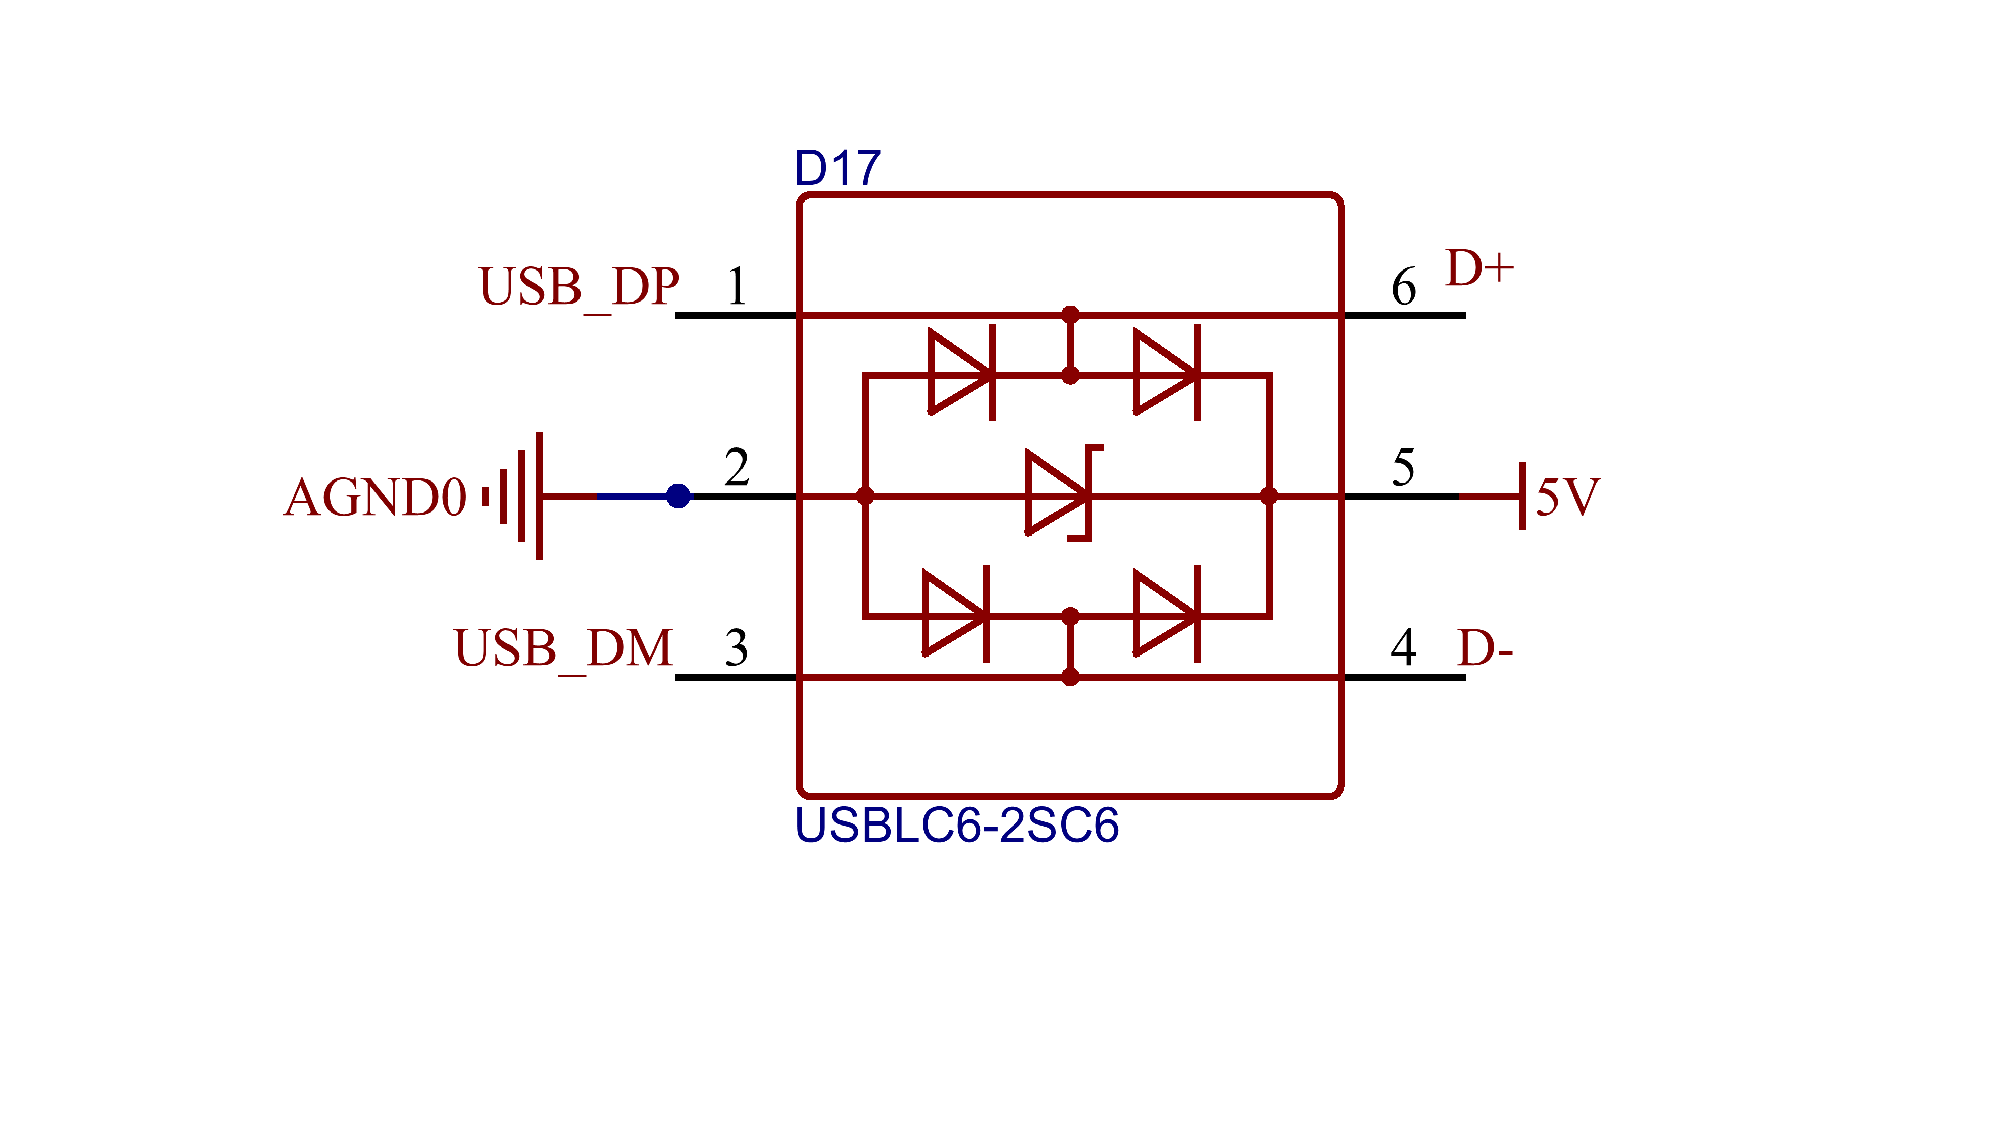
\includegraphics[width=0.28\textheight]{USB_ESD.pdf}
	\caption{USBLC6-2SC6原理图} 
	\label{fig2-17}
\end{figure}


(2) USB输入端引入USBLC6-2SC6进行ESD保护。USBLC6-2SC6是意法半导体公司为USB通讯电路设计的专用ESD保护芯片,其能够同时保护两条USB通信线路,I/O与地之间的电容匹配公差仅为0.015 pF,典型电容值不超过3.5 pF,符合USB 2.0的通讯需求。USBLC6-2SC6能够为设备提供$\pm8$ kV的接触和$\pm15$ kV空气间隙放电保护。其原理图如图\ref{fig2-17}所示。

(3) 为了避免静电经由开关进入PCB,在开关处引入PSOT05C-LF-T7芯片。PSOT05C-LF-T7为PROTEK公司设计的TVS二极管阵列,被广泛应用于电源线路保护。其能够在3 V-36 V的电压下工作,为系统提供$\pm8$ kV的接触和$\pm15$ kV空气间隙放电保护。同时其能够承受500 W的峰值脉冲功率(上升沿8 us,半峰值20 us下),符合设计要求。其原理图如图\ref{fig2-18}所示。

\begin{figure}[h]
	\centering
	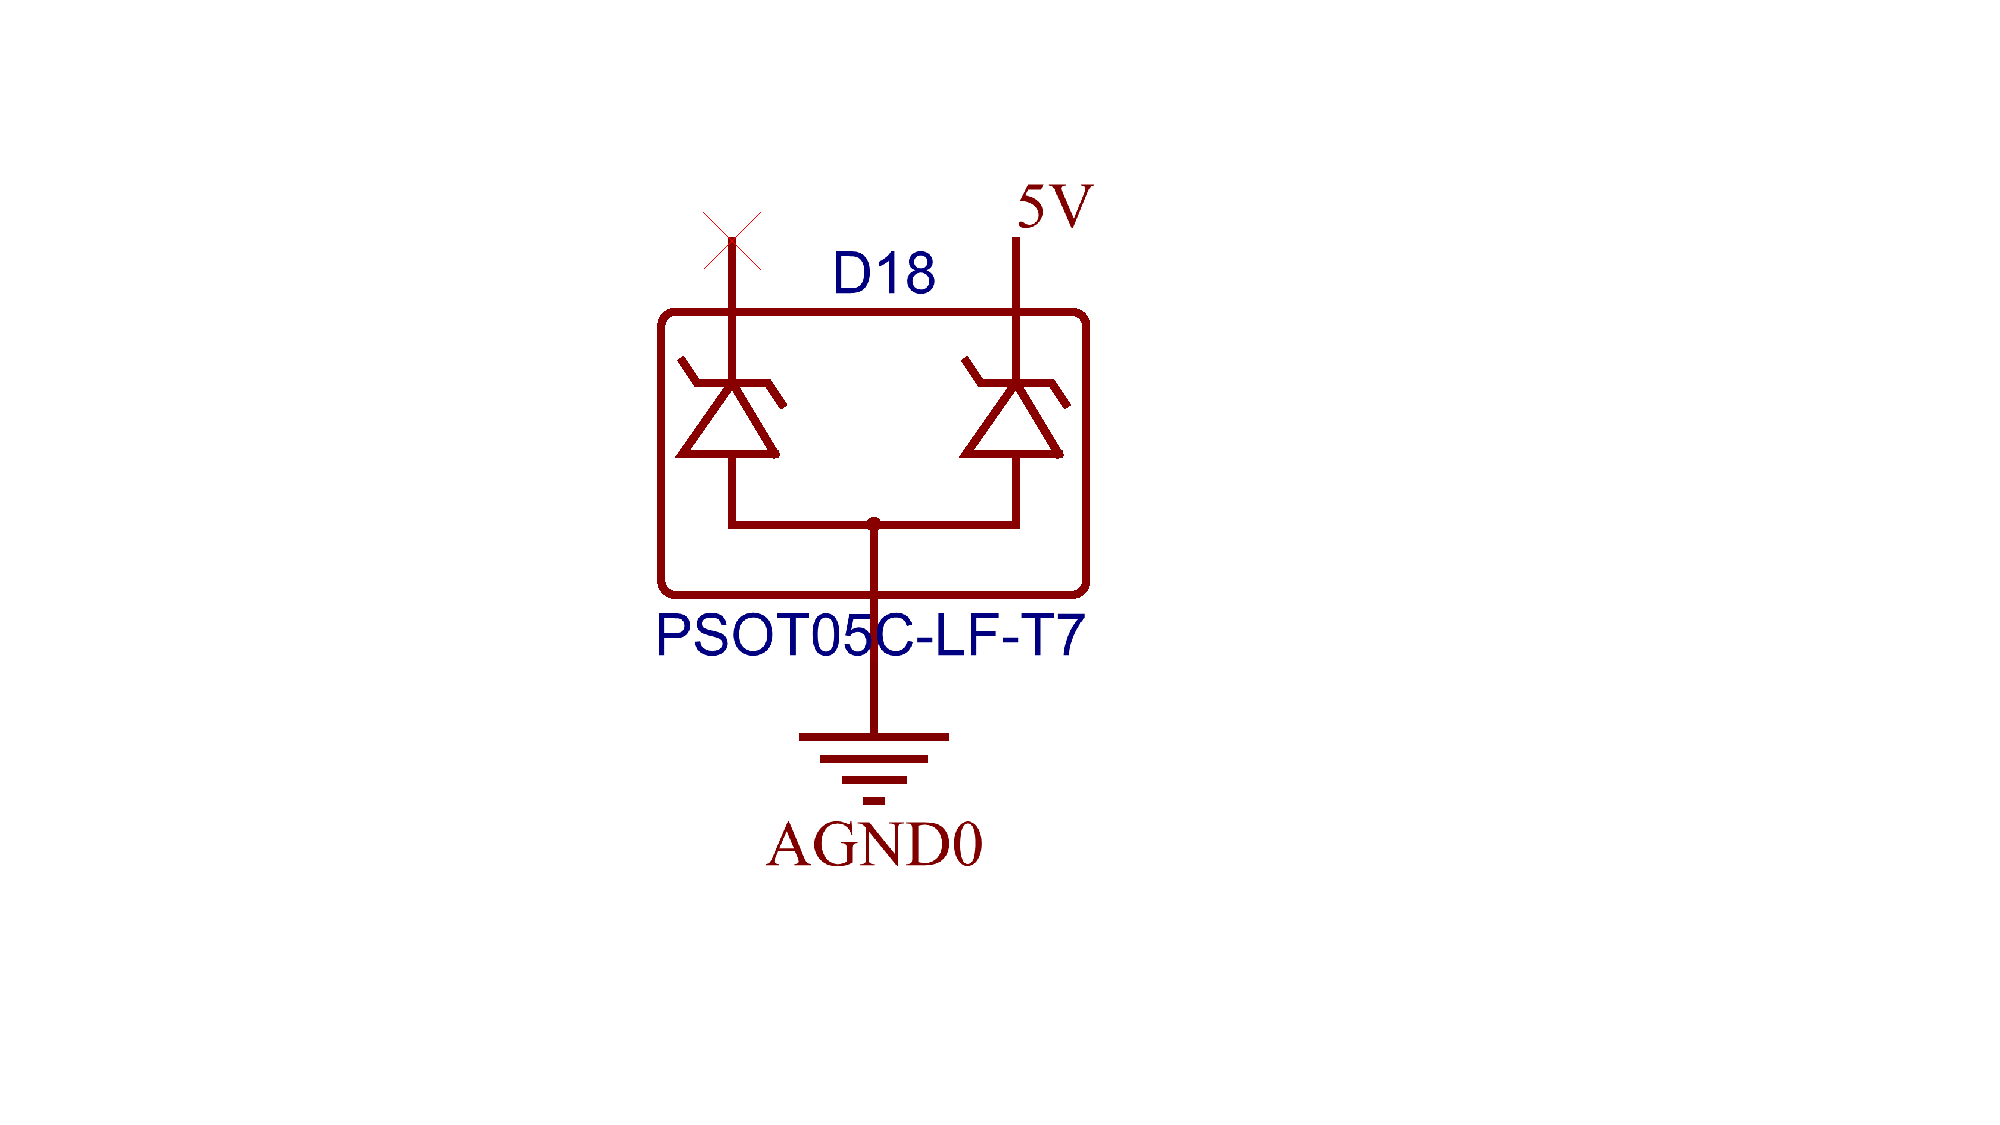
\includegraphics[width=0.08\textheight]{开关ESD.pdf}
	\caption{PSOT05C-LF-T7原理图} 
	\label{fig2-18}
\end{figure}

为保证设备能够在过载情况下进行自我保护,防止芯片损坏,在USB端口的供电处设计了自恢复保险丝。保险丝型号的选取考虑以下两点:(1) 采集模块的工作电流。测量得到采集模块正常工作时的电流为285 mA,与计算值基本相符。(2) USB端口供电能力。USB 2.0端口的供电能力为5 V/500 mA。综上所述,选取ASMD1210-050作为保险丝,其熔断电流为500 mA,符合设计需求。



\section{JS-AINS-40系统软件设计}
在硬件内容的基础上,本节介绍JS-AINS-40系统配套的软件设计。软件设计主要包括采集模块的下位机软件和上位机的软件两部分,其中下位机软件运行在STM32H743IIT6的嵌入式平台,上位机软件运行在Windows PC端。
\subsection{下位机软件设计}
利用C语言编写的下位机软件主要实现的功能包括:通过STM32H743IIT6主控模块经由SPI隔离模块控制ADS1299采集模块,使其按照性能要求采集EEG数据。接收ADS1299采集模块回传的数据,裁剪拼接后通过虚拟串口通讯模传递给上位机。

(1) STM32H743IIT6主控模块主程序

\begin{figure}[h]
	\centering
	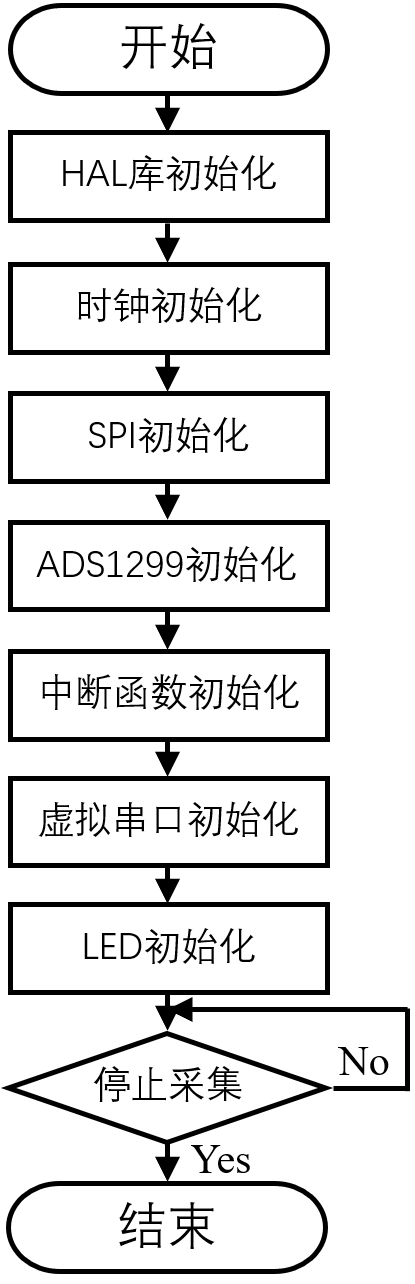
\includegraphics[width=0.13\textheight]{下位机主程序.png}
	\caption{STM32H743IIT6主控模块主程序流程图} 
	\label{fig2-19}
\end{figure}

STM32H743IIT6主控模块主程序主要负责进行初始化。其首先初始化STM32H743IIT6芯片的HAL库和时钟,保证主控芯片开始正常运行。之后初始化SPI模块,保证主控芯片能够通过SPI初始化ADS1299。ADS1299初始化时,STM32H743IIT6主控芯片将根据具体的使用需求配置ADS1299的内部寄存器,保证其正常采集。中断函数和虚拟串口初始化后将保证主控芯片能够识别ADS1299发来的数据转换完成信号,并将接收到的数据发送给上位机。最后,LED初始化后将作为设备工作状态的指示灯。具体流程如图\ref{fig2-19}所示。

在所有设备初始化结束后,主控芯片将自动读取每一片ADS1299的控制寄存器,确认其是否与初始化时设置的一致。如果存在差异,则LED指示灯将通过不同次数的闪烁告知使用者出现问题的ADS1299编号,并通过虚拟串口向上位机发送提示使用者进行设备重启的字符。如果不存在差异,则认为设备正常启动,向上位机发送已准备就绪的字符,并进入准备状态,等待运行指令。


(2) ADS1299 控制程序

主控芯片通过SPI初始化ADS1299的流程为:

1) 拉低RESET引脚,对ADS1299进行复位,并在20 ms后拉高RESET引脚。在间隔20 ms后再次拉低RESET引脚,并在20 ms后拉高RESET引脚。重复执行这一过程,是为了保证ADS1299复位成功。(这期间,START引脚始终保持低电平)

2) 向第一片ADS1299芯片发送停止连续读取指令,并停顿20 ms,保证指令生效。

3) 向第一片芯片发送控制寄存器1的配置指令。寄存器1负责控制多芯片的级联方式,是否向外输出内部时钟以及EEG数据的采样率。根据硬件设计章节的叙述,这里选择使用标准配置来级联多块ADS1299,因此寄存器1设置为多重回读模式(Multiple Readback Mode)。同时,由于第一块ADS1299芯片作为主芯片需要给从属芯片提供时钟,因此这里设置向外输出内部时钟。最后,EEG信号的采样率根据任务要求具体设置。注意,这一步骤结束后需要等待50 ms,以保证主芯片的时钟趋于稳定,这时才能够成功初始化从属芯片。

4) 向所有从属ADS1299芯片发送停止连续读取指令,并停顿20 ms,保证指令生效。

5) 向所有从属ADS1299芯片发送控制寄存器1的配置指令。从属芯片接收外来时钟,因此配置与主芯片略有不同。

6) 向第一片芯片发送控制寄存器3的配置指令。控制寄存器3负责右腿驱动模块的设置,基于硬件设计章节的叙述,开启主ADS1299芯片的右腿驱动电路。

7) 向所有从属ADS1299芯片发送控制寄存器3的配置指令,关闭其右腿驱动电路。

8) 对剩余所有控制寄存器配置,主从ADS1299芯片均保持一致。按照要求依次在对应控制寄存器中配置工作模式(正常电极输入)、差分输入模式(共差分输入,SRB1作为公共端)、参考类型(使用内部参考)、PGA增益(本章设计时选取24)。

9) 发送连续转换指令,进入准备状态。

经过上述流程,ADS1299被成功初始化。在STM32H743IIT6芯片接收到上位机发送的运行指令后,将把ADS1299的START引脚拉高,使其开始信号采集与模数转化。当一次模数转化完成后,ADS1299的DRDY引脚被拉低,进而触发在STM32H743IIT6芯片的中断程序。

(3) 中断程序

STM32H743IIT6主控芯片将主ADS1299芯片的DRDY引脚设置为外部中断源。当进入中断程序时,主控芯片会依次读取五块ADS1299的全部数据。每片ADS1299的数据有216 bits,其中前24位为芯片状态位(1100 + LOFF\_STATP + LOFF\_STATN + GPIO寄存器的4-7位),后192位为8个通道的EEG数据。每个通道的数据由24位补码表示,根据数据手册,其中一位的分辨率(Least Sigificant Bit,LSB)为:

\begin{equation}
    \label{deqn_ex2_3}
    1\ \mathrm{LSB}=\left(2 \times \mathrm{V}_{\mathrm{REF}} / \text { Gain }\right) / 2^{24}=+\mathrm{FS} / 2^{23}
\end{equation}

其中$\mathrm{V}_{\mathrm{REF}}$为参考电压(本章设计中为4.5 V),$\text{Gain}$为PGA增益(本章设计时选取24),$-\mathrm{FS}$至$+\mathrm{FS}$为ADS1299的采集范围。不同的信号幅度与对应输出结果间的关系如表\ref{tab2-1}:

\begin{table*}[!h]
\caption{输入信号幅度与转换结果对应关系}  \label{tab2-1}
\centering
\wuhao{
    \begin{threeparttable}
    \setlength{\tabcolsep}{5mm}{
        \begin{tabular}{cc}
            \toprule
            信号幅度 &转换结果\\
            \midrule
            $\geq F S$                                 &7FFFFFh \\
            $+F S /\left(2^{23}-1\right)$              &000001h \\
            0                                          &0 \\
            $-F S /\left(2^{23}-1\right)$              &FFFFFFh  \\
            $\leq-F S\left(2^{23} / 2^{23}-1\right)$   &800000h\\
            \bottomrule
        \end{tabular}
        }
    \end{threeparttable}
    }
\end{table*}

本设计并不关心芯片状态位,因此直接舍去前24位,仅保留每个芯片的后192位数据进行拼接,并通过虚拟串口发送函数发送给上位机。考虑到下位机的计算资源有限,输入信号的幅度转换放置在上位机中进行。

(4) 虚拟串口通讯程序

STM32CubeMX软件由意法半导体公司开发,作为STM32芯片配套的辅助开发工具。其能够通过图形化的界面快速生成相应的程序代码,大幅简化开发流程。因此在本节,使用STM32CubeMX软件生成相应的虚拟串口通讯程序。具体设置流程为:首先,选择STM32H743IIT6芯片;之后在外设界面选择添加USB,并选取FS通道;接下来添加中间件,选择CDC虚拟串口;最后,设置时钟并生成工程代码。利用生成的工程模板中的虚拟串口发送函数,即可实现向上位机的数据发送。由于虚拟串口每次发送需要消耗一定的时间,这在ADS1299处于高采样率时可能导致数据丢包。因此,主控芯片会将每个DRDY中断后得到的EEG数据暂时进行存储,在中断次数达到8次后统一进行发送,即传输960(8 × 5 × 24)字节的数据。为了保证数据传输的完整性,在960字节数据末尾添加CRC校验位——由下位机计算CRC校验值后,一次向上位机发送961字节数据。

\subsection{上位机软件设计}

上位机程序能够向使用者反馈下位机的当前状态,引导使用者进行设备重启或者开始采集、能够操控采集设备的启动与停止、能够接收下位机传送的EEG数据并进行幅度转换、能够根据转换后的EEG数据实时绘制波形图、能够在接收EEG数据时同步保存转换后的EEG数据,并且能够配合EEG实验引导界面为EEG数据进行标签标注。软件界面如图\ref{fig2-20}所示。具体使用流程为:

\begin{figure}[h]
	\centering
	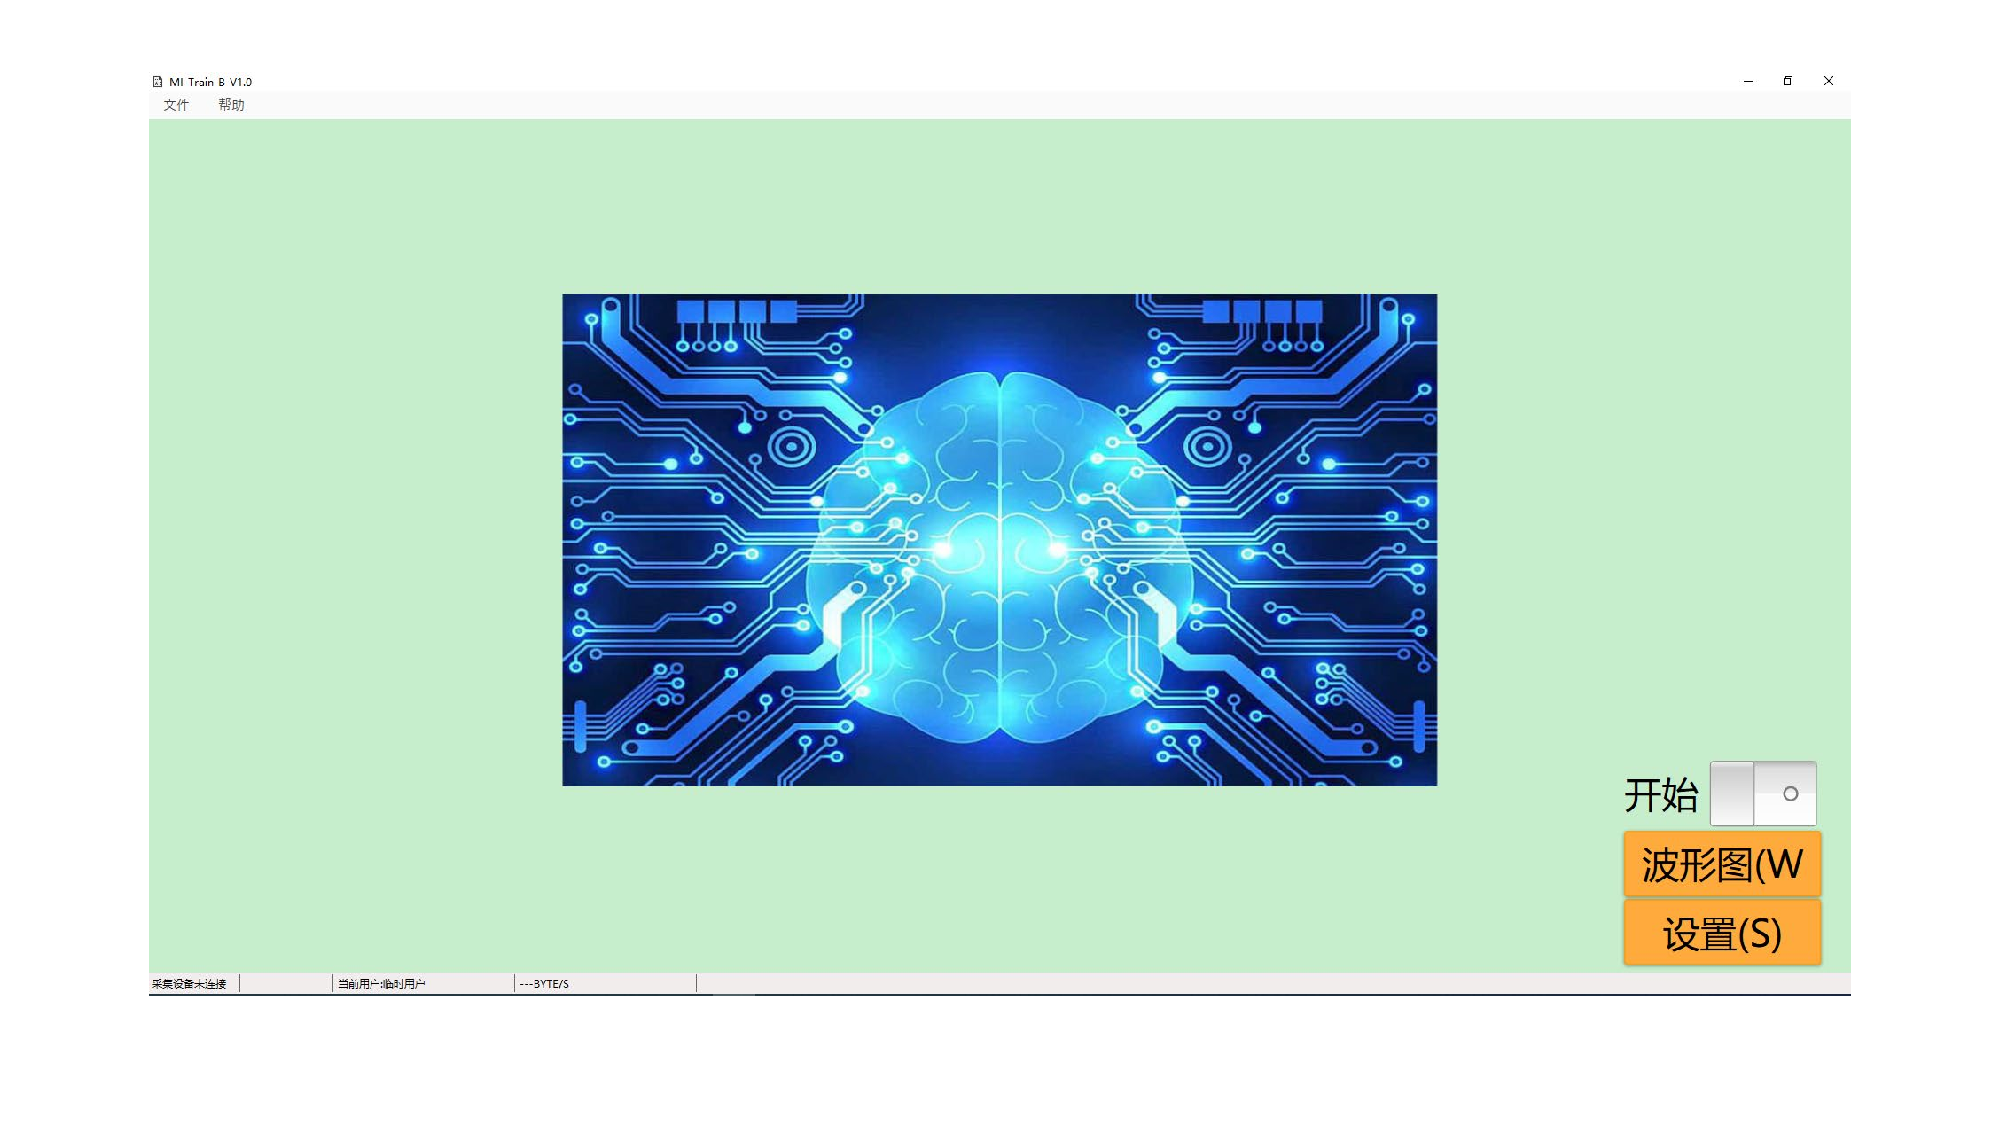
\includegraphics[width=0.6\textheight]{软件界面.pdf}
	\caption{上位机主界面} 
	\label{fig2-20}
\end{figure}

(1) 点击右下角设置按钮,在串口设置中选取下位机设备的串口号,在存储设置中选取EEG数据的目标存储位置。

(2) 设置完成后,点击文件下拉菜单中的打开串口按钮。这时下位机会向上位机发送准备就绪/需要重启的字符,引导使用者进行操作。

(3) 当设备准备就绪后,主界面左下角会出现采集设备已连接的提示。使用者点击主界面的开始按钮,上位机就会向下位机发送启动命令,下位机拉高ADS1299的START引脚,开始数据采集。

(4) 接收到数据后,上位机首先通过CRC校验位检查数据完整性。如果校验正确,则继续接收数据。如果校验失败,则暂停采集并提示使用者数据出错。

(5) 采集过程中,可以选择开启波形图实时观察采集信号。采集过程中的波形图如图\ref{fig2-21}所示。

\begin{figure}[h]
	\centering
	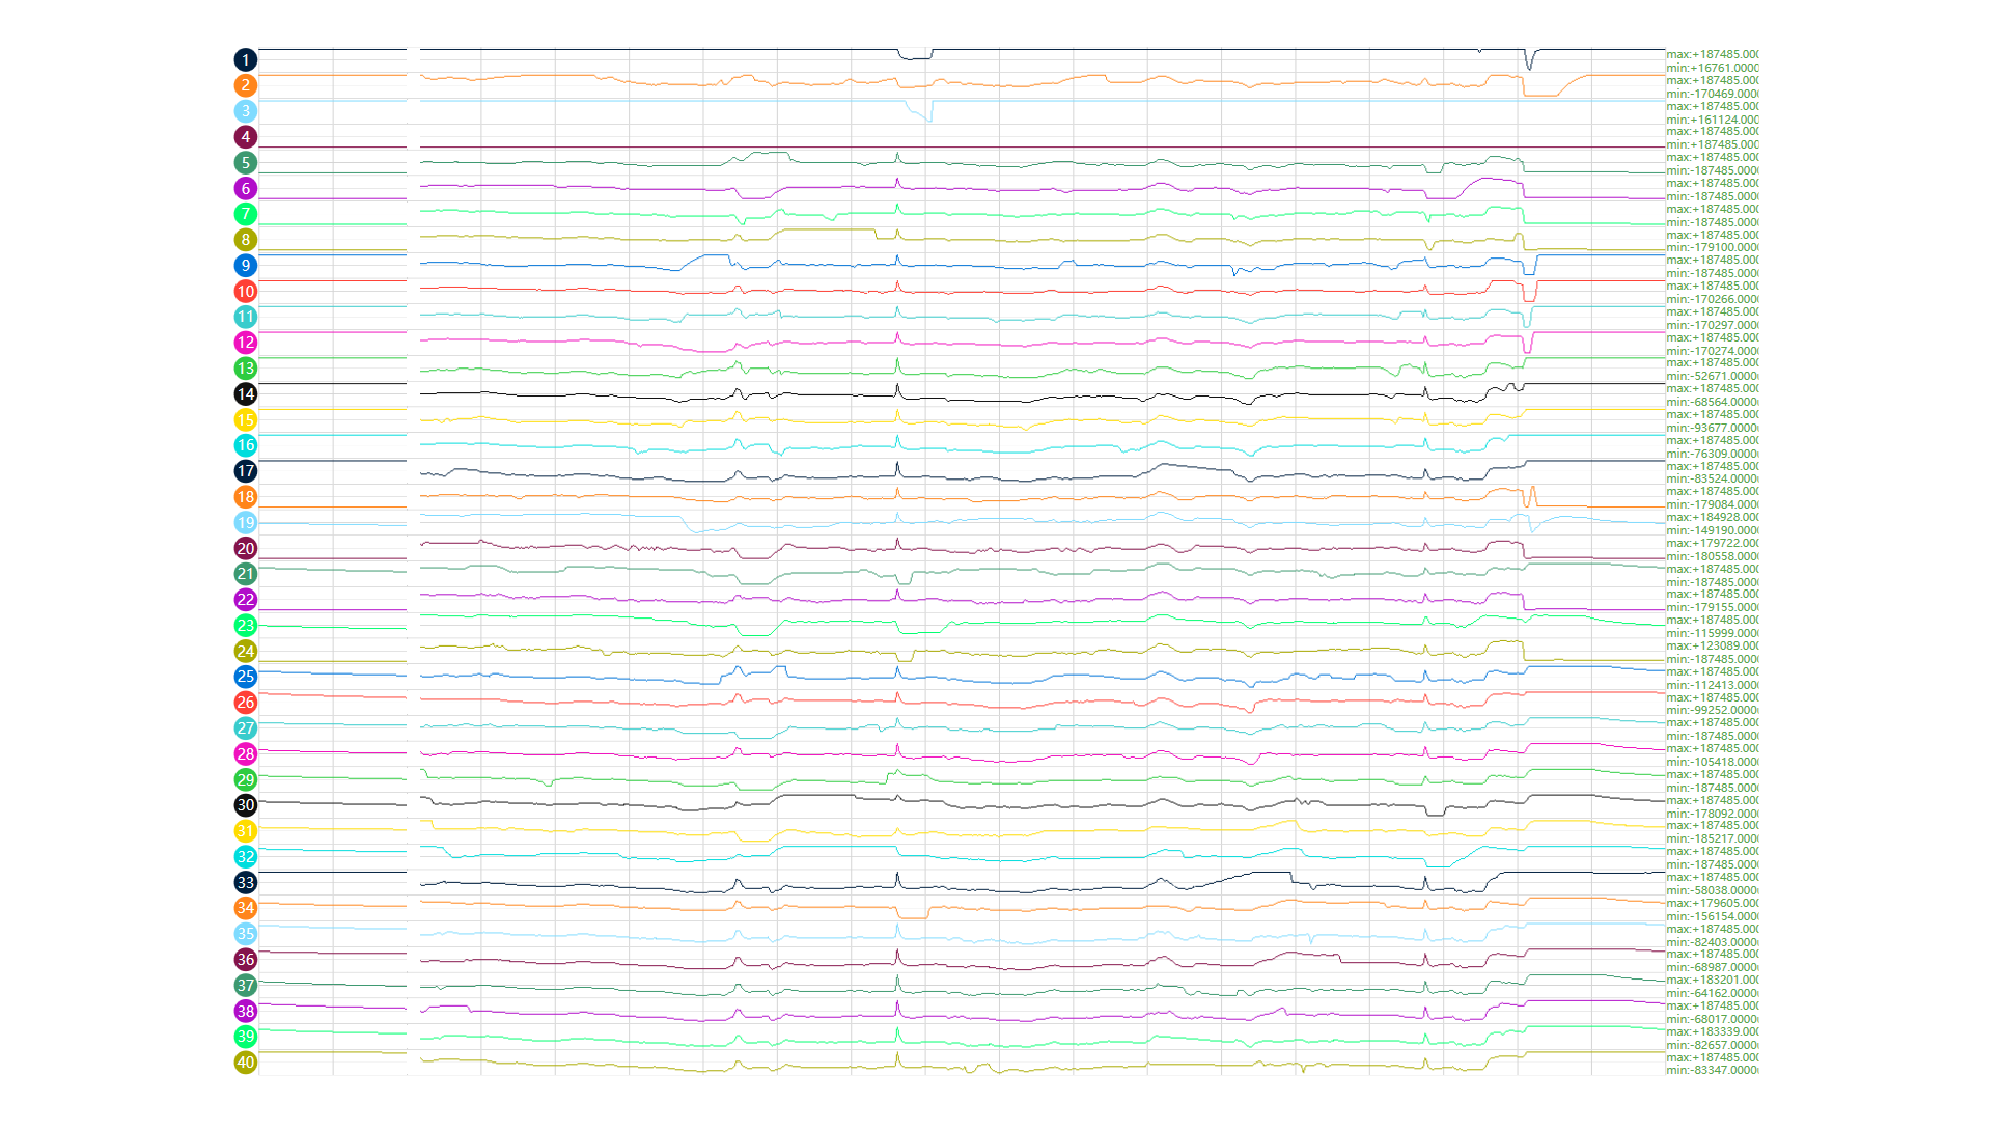
\includegraphics[width=0.52\textheight]{波形图界面.pdf}
	\caption{EEG波形图界面} 
	\label{fig2-21}
\end{figure}

(6) 采集结束后,关闭波形图界面,再次点击开始按钮,上位机会向下位机发送停止命令,下位机拉低ADS1299的START引脚,停止数据采集。

在给出具体需求和与下位机的通信方式后,上位机程序由深圳市缔峰泽公司实现编写。

\section{JS-AINS-40系统性能测试}
脑电采集设备在投入使用前需要经过严格的性能测试,以保证信号采集的准确有效。本节遵照中华人民共和国国家计量与检定规程JJG954-2019《数字脑电图仪》和中华人民共和国国家标准GB9706.226-2021《医用电气设备》中的步骤和要求进行性能检定。主要检定内容包括:电压测量、共模抑制比、噪声电平以及电磁兼容测试。

\subsection{电压测量}
电压测量遵循JJG954-2019《数字脑电图仪》中的要求,并使用SKX-8000微弱信号发生器来模拟检定仪与衰减器的输出。将不同幅值的0.1 s周期方波信号分别输入被检通道,记录30 s内波形幅值偏离最大者,并计算电压测量相对误差$\delta_{\mathrm{m}}$,其公式如下:
\begin{equation}
    \label{deqn_ex2_4}
    \delta_{\mathrm{m}}=\frac{U_{\mathrm{m}}-U_{\text {in }}}{U_{\text {m }}} \times 100 \%
\end{equation}

其中$U_{\mathrm{m}}$为偏离SKX-8000微弱信号发生器输入电压$U_{\text {in }}$的最大电压测量值。电压测量最大允许误差为$\pm 10 \times\left(1+\frac{U_1}{U_{\text {in}}}\right) \%$,其中$U_1$为设备当前灵敏度的五倍。JS-AINS-40系统的最高灵敏度为0.02 $\mu $V,考虑到JJG954-2019中要求的测试信号幅值远大于0.02 $\mu $V,这里直接使用$\pm 10\%$作为测量误差上界。

最终JS-AINS-40系统在不同输入电压下的测量相对误差如表\ref{tab2-2}所示。表中给出了每次测量所有通道中最大的相对误差值,可以看到,所有结果均在$\pm 10\%$以下,符合国标要求。

\begin{table}[!h]
	\centering
	\caption{电压测量相对误差}
	\wuhao{
			\begin{tabular}{cccccc}
			\toprule
			检定仪输出/  $\mu $V  & 相对误差   &检定仪输出/  $\mu $V  & 相对误差   &检定仪输出/  $\mu $V  & 相对误差   \\ 
			\midrule
			 10   & 9.2\%   &  50   & 5.9\%  &  500   &  0.9\%\\ 
			 20  & 7.4\%   &  100  & 3.5\%  &  1000  &  0.5\%\\ 
			 25  & 6.8\%   &  200  & 1.6\%  &  2000  &  0.4\%\\
			\bottomrule
		\end{tabular}
	}
	\label{tab2-2}
\end{table}

\subsection{共模抑制比}

基于前文所述,JS-AINS-40系统基于差模输入的方式采集EEG信号,而外部噪声基本以共模形式进入采集设备。因此,JS-AINS-40系统需要具备足够的共模抑制比来降低噪声对EEG信号的干扰。本节依然使用SKX-8000微弱信号发生器来模拟检定仪与衰减器的输出。遵照JJG954-2019,首先向JS-AINS-40系统输入50 Hz,幅值为200 $\mu$V的差模信号(JS-AINS-40系统的采集电极连接信号源正极,参考电极和右腿驱动电极连接信号源负极),记录差模信号幅值$U_d$。向JS-AINS-40系统输入50 Hz,幅值为2 V的共模信号(JS-AINS-40系统的采集电极和参考电极连接信号源正极,右腿驱动电极连接信号源负极),记录共模信号幅值$U_c$。按照公式\ref{deqn_ex2_5}计算所有通道的共模抑制比。

\begin{equation}
    \label{deqn_ex2_5}
    C M R R = 20 \lg K + 20 \lg\frac{U_{\mathrm{d}}}{U_{\mathrm{c}}}
\end{equation}

\begin{figure}[!h]
	\centering
	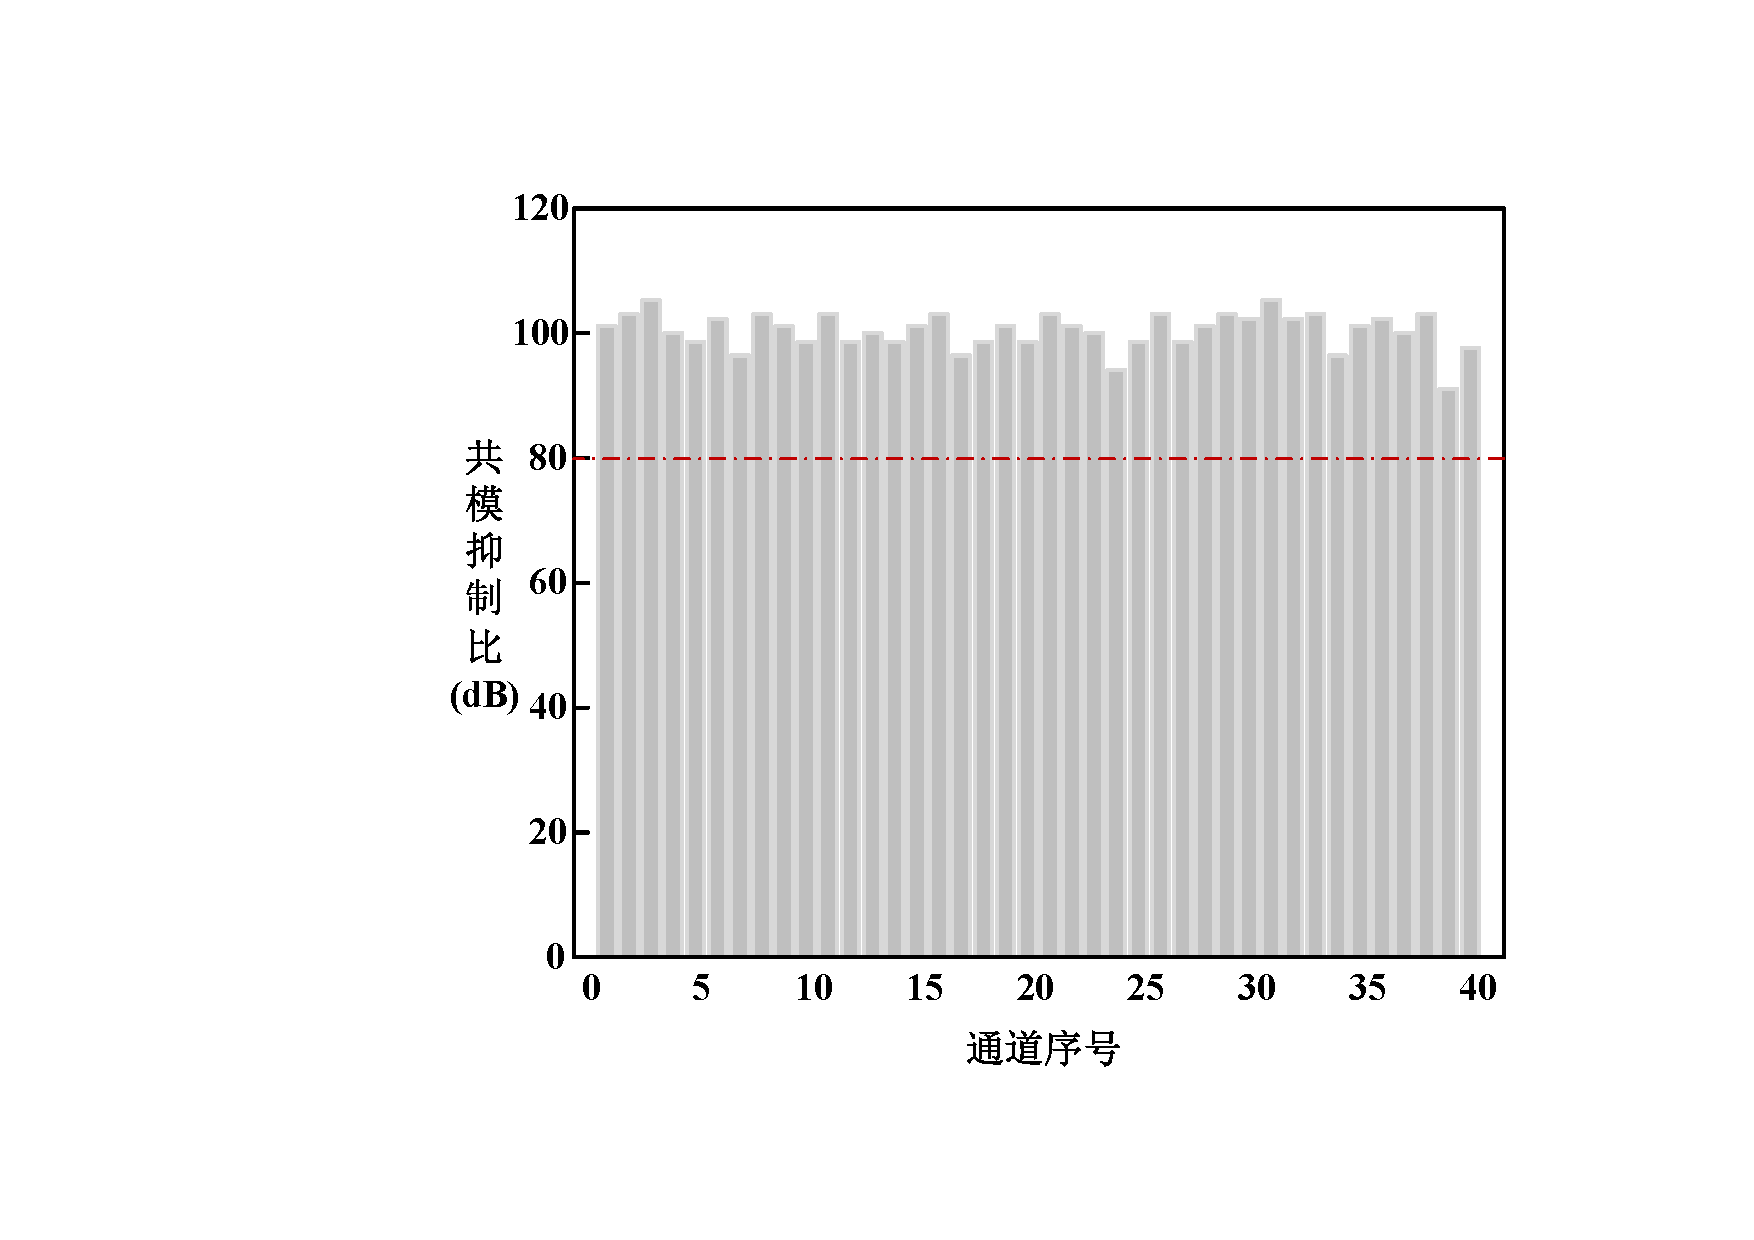
\includegraphics[width=0.37\textheight]{共模抑制比.pdf}
	\caption{通道的共模抑制比} 
	\label{fig2-23}
\end{figure}
其中$K$为SKX-8000输入的共模信号电压与差模信号电压比值。得到四十个通道的共模抑制比如图\ref{fig2-23}所示,可以看到,所有通道的共模抑制比均大于80 dB,符合国标要求。



\subsection{噪声电平}
JJG954-2019中对于噪声电平的定义为:采集设备的各通道输入端对地短接时,采集到的10 s噪声信号幅值。根据这一定义,本节将设备所有采集电极,参考电极和右腿驱动电极短接至屏蔽地,而后开始信号采集,并记录其幅度值。40个通道的噪声如图\ref{fig2-24}所示,可以看到所有通道噪声的最大幅值均在6 $\mu$V以内,符合GB9706.226-2021国标要求。
\begin{figure}[!h]
	\centering
	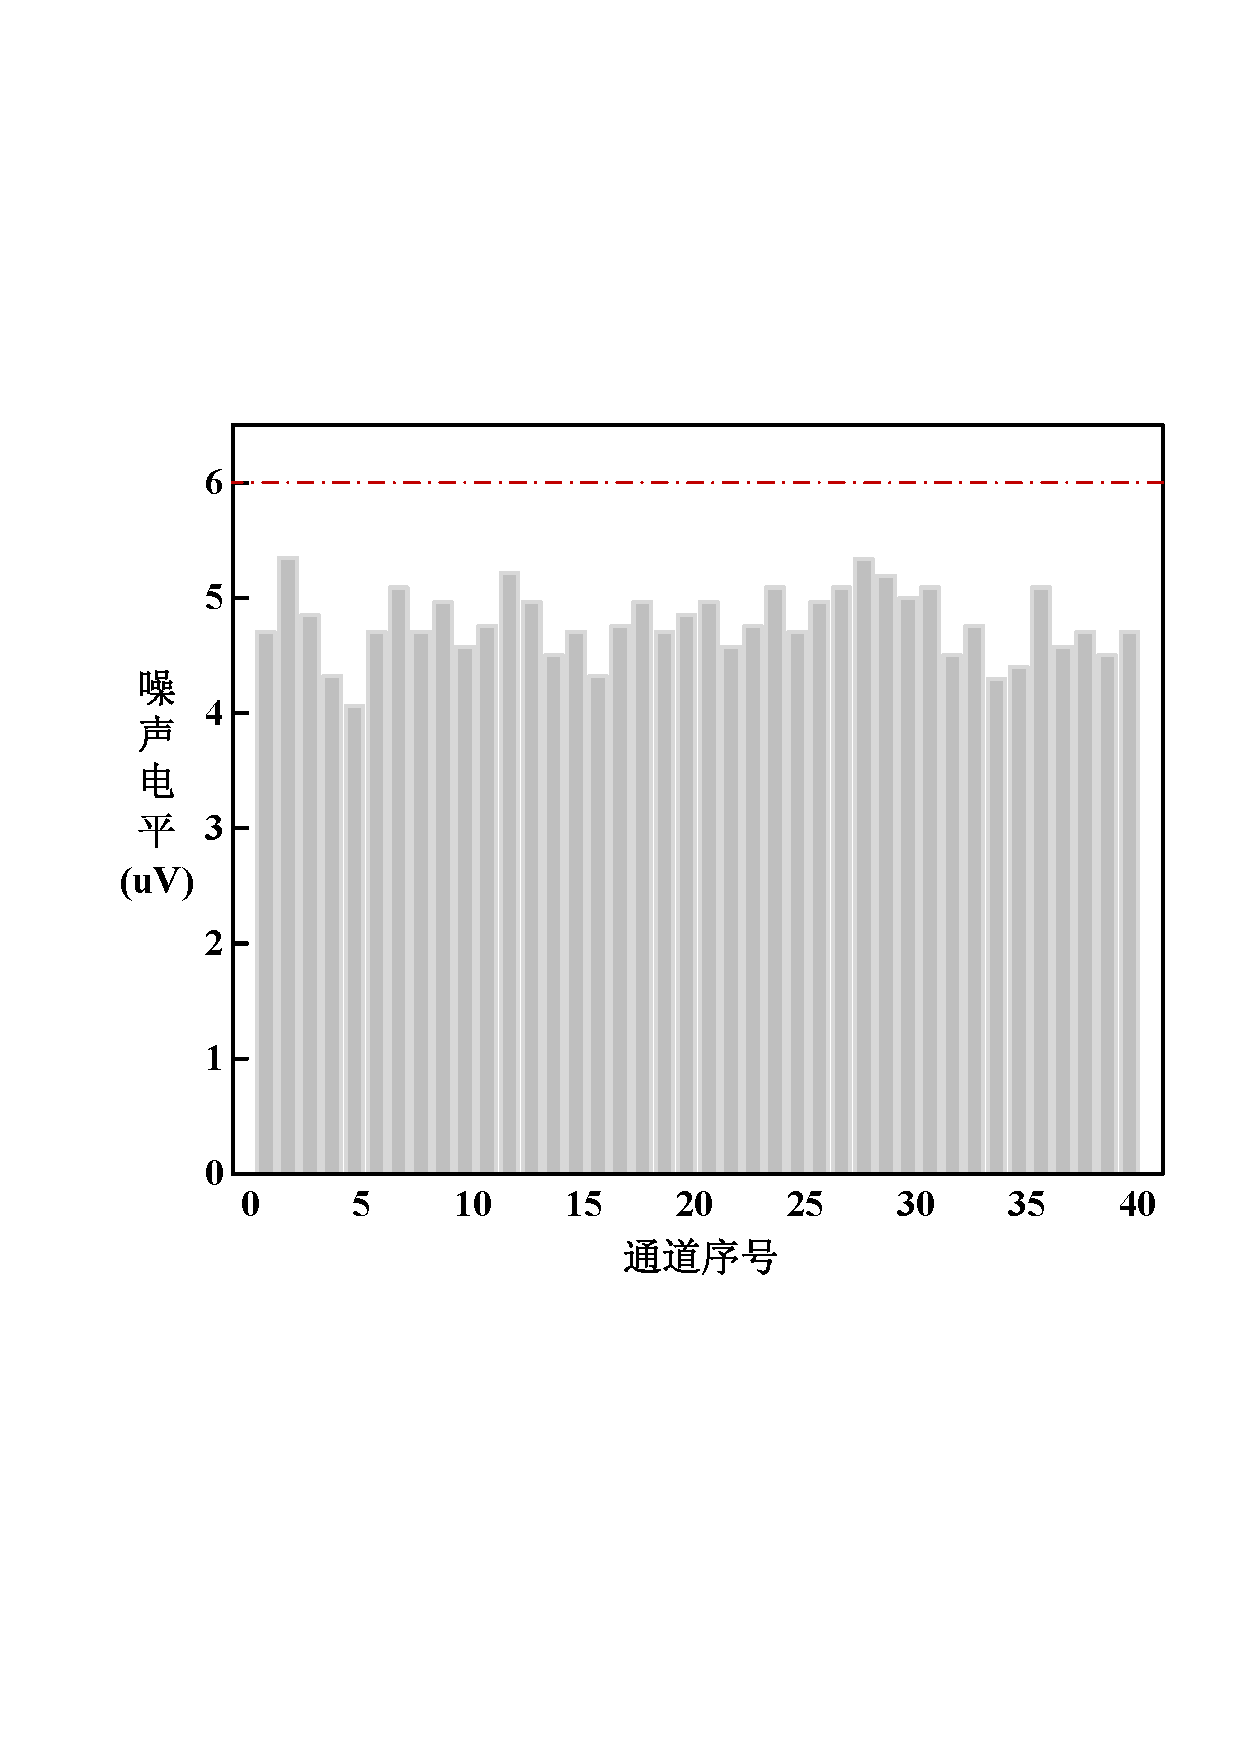
\includegraphics[width=0.37\textheight]{噪声.pdf}
	\caption{通道噪声电平} 
	\label{fig2-24}
\end{figure}

\subsection{电磁兼容测试}
JS-AINS-40系统作为一种电子设备,其需要在常规电磁环境中正常运行,并且不能对其他电子产品造成无法忍受的电磁干扰。因此,本节对其进行了电磁兼容测试(Electro Magnetic Compatibility,EMC)。进行的测试包括:静电测试、辐射发射测试以及射频场感应的传导骚扰抗扰度测试。静电测试和传导抗扰度测试的现场如图\ref{fig2-25}所示。

\begin{figure}[!h]
	\centering
	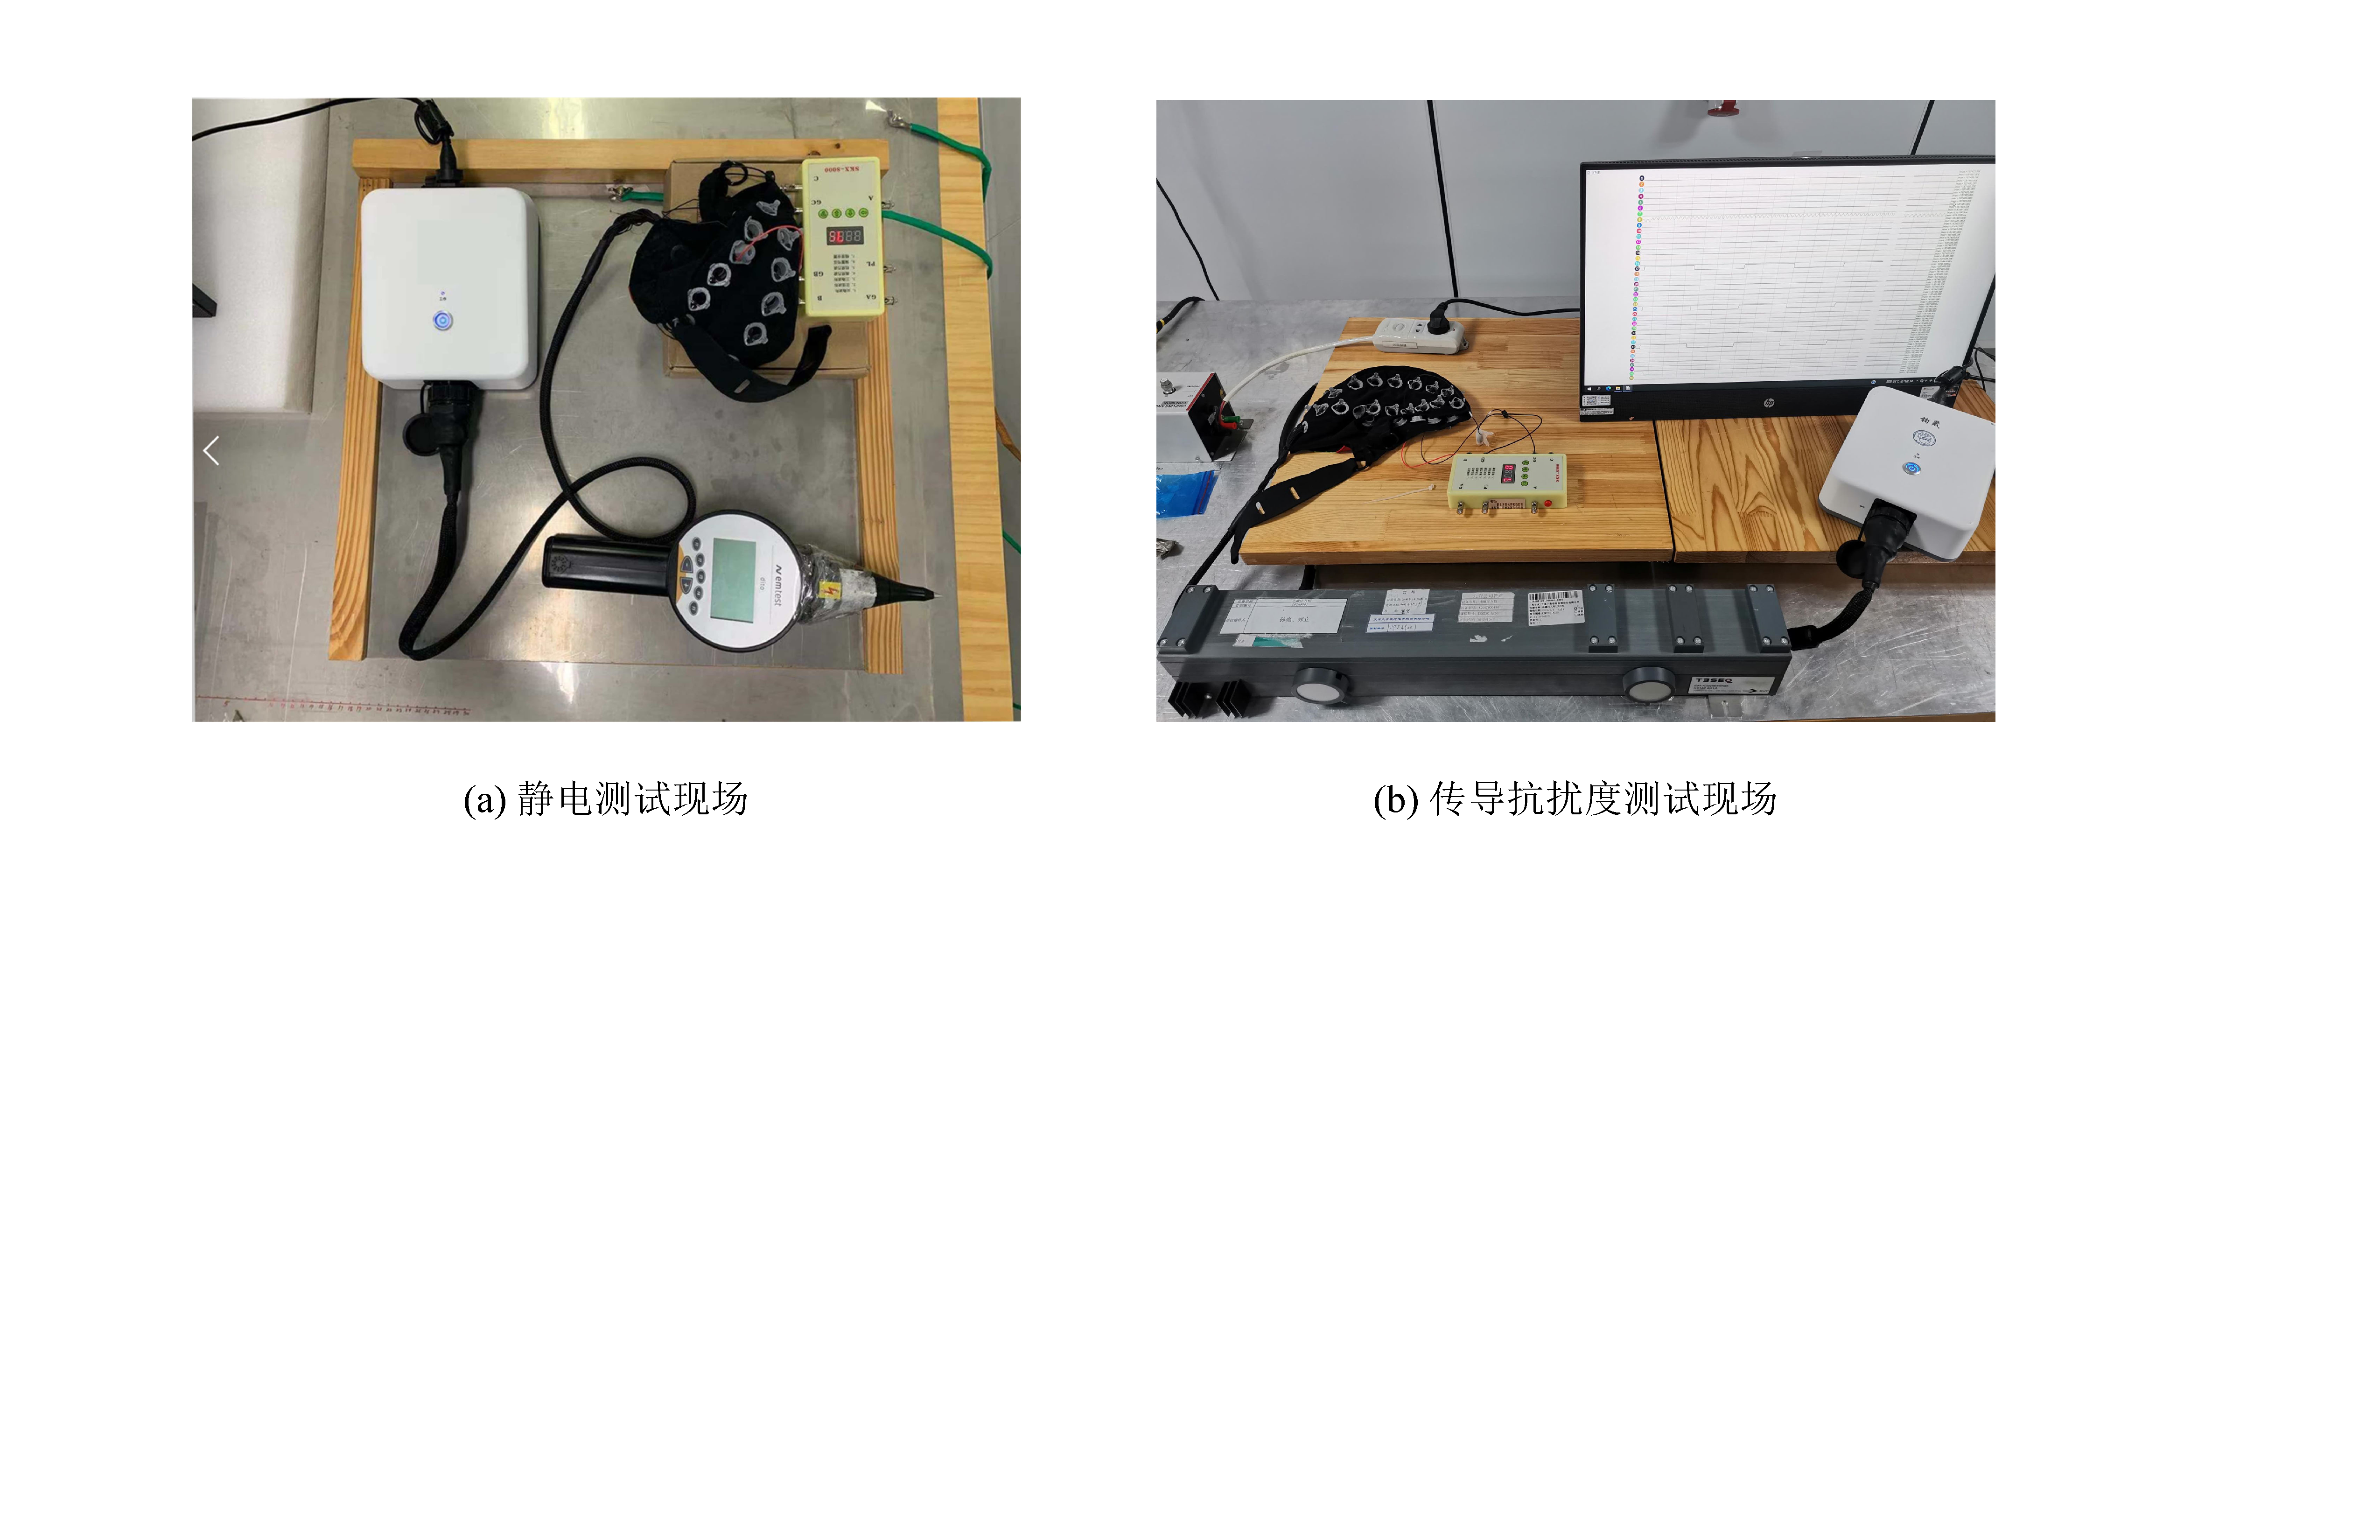
\includegraphics[width=0.60\textheight]{EMC.pdf}
	\caption{EMC测试现场} 
	\label{fig2-25}
\end{figure}

在测试中,JS-AINS-40系统能够承受8 kV的空气放电和6 kV的接触放电,符合静电测试要求;同时,JS-AINS-40系统在150 kHz至80 MHz的频率范围内,能够承受3类实验等级的射频发射机传导线电磁骚扰,符合国标要求的医疗设备抗扰度要求。


\begin{figure}[!h]
	\centering
	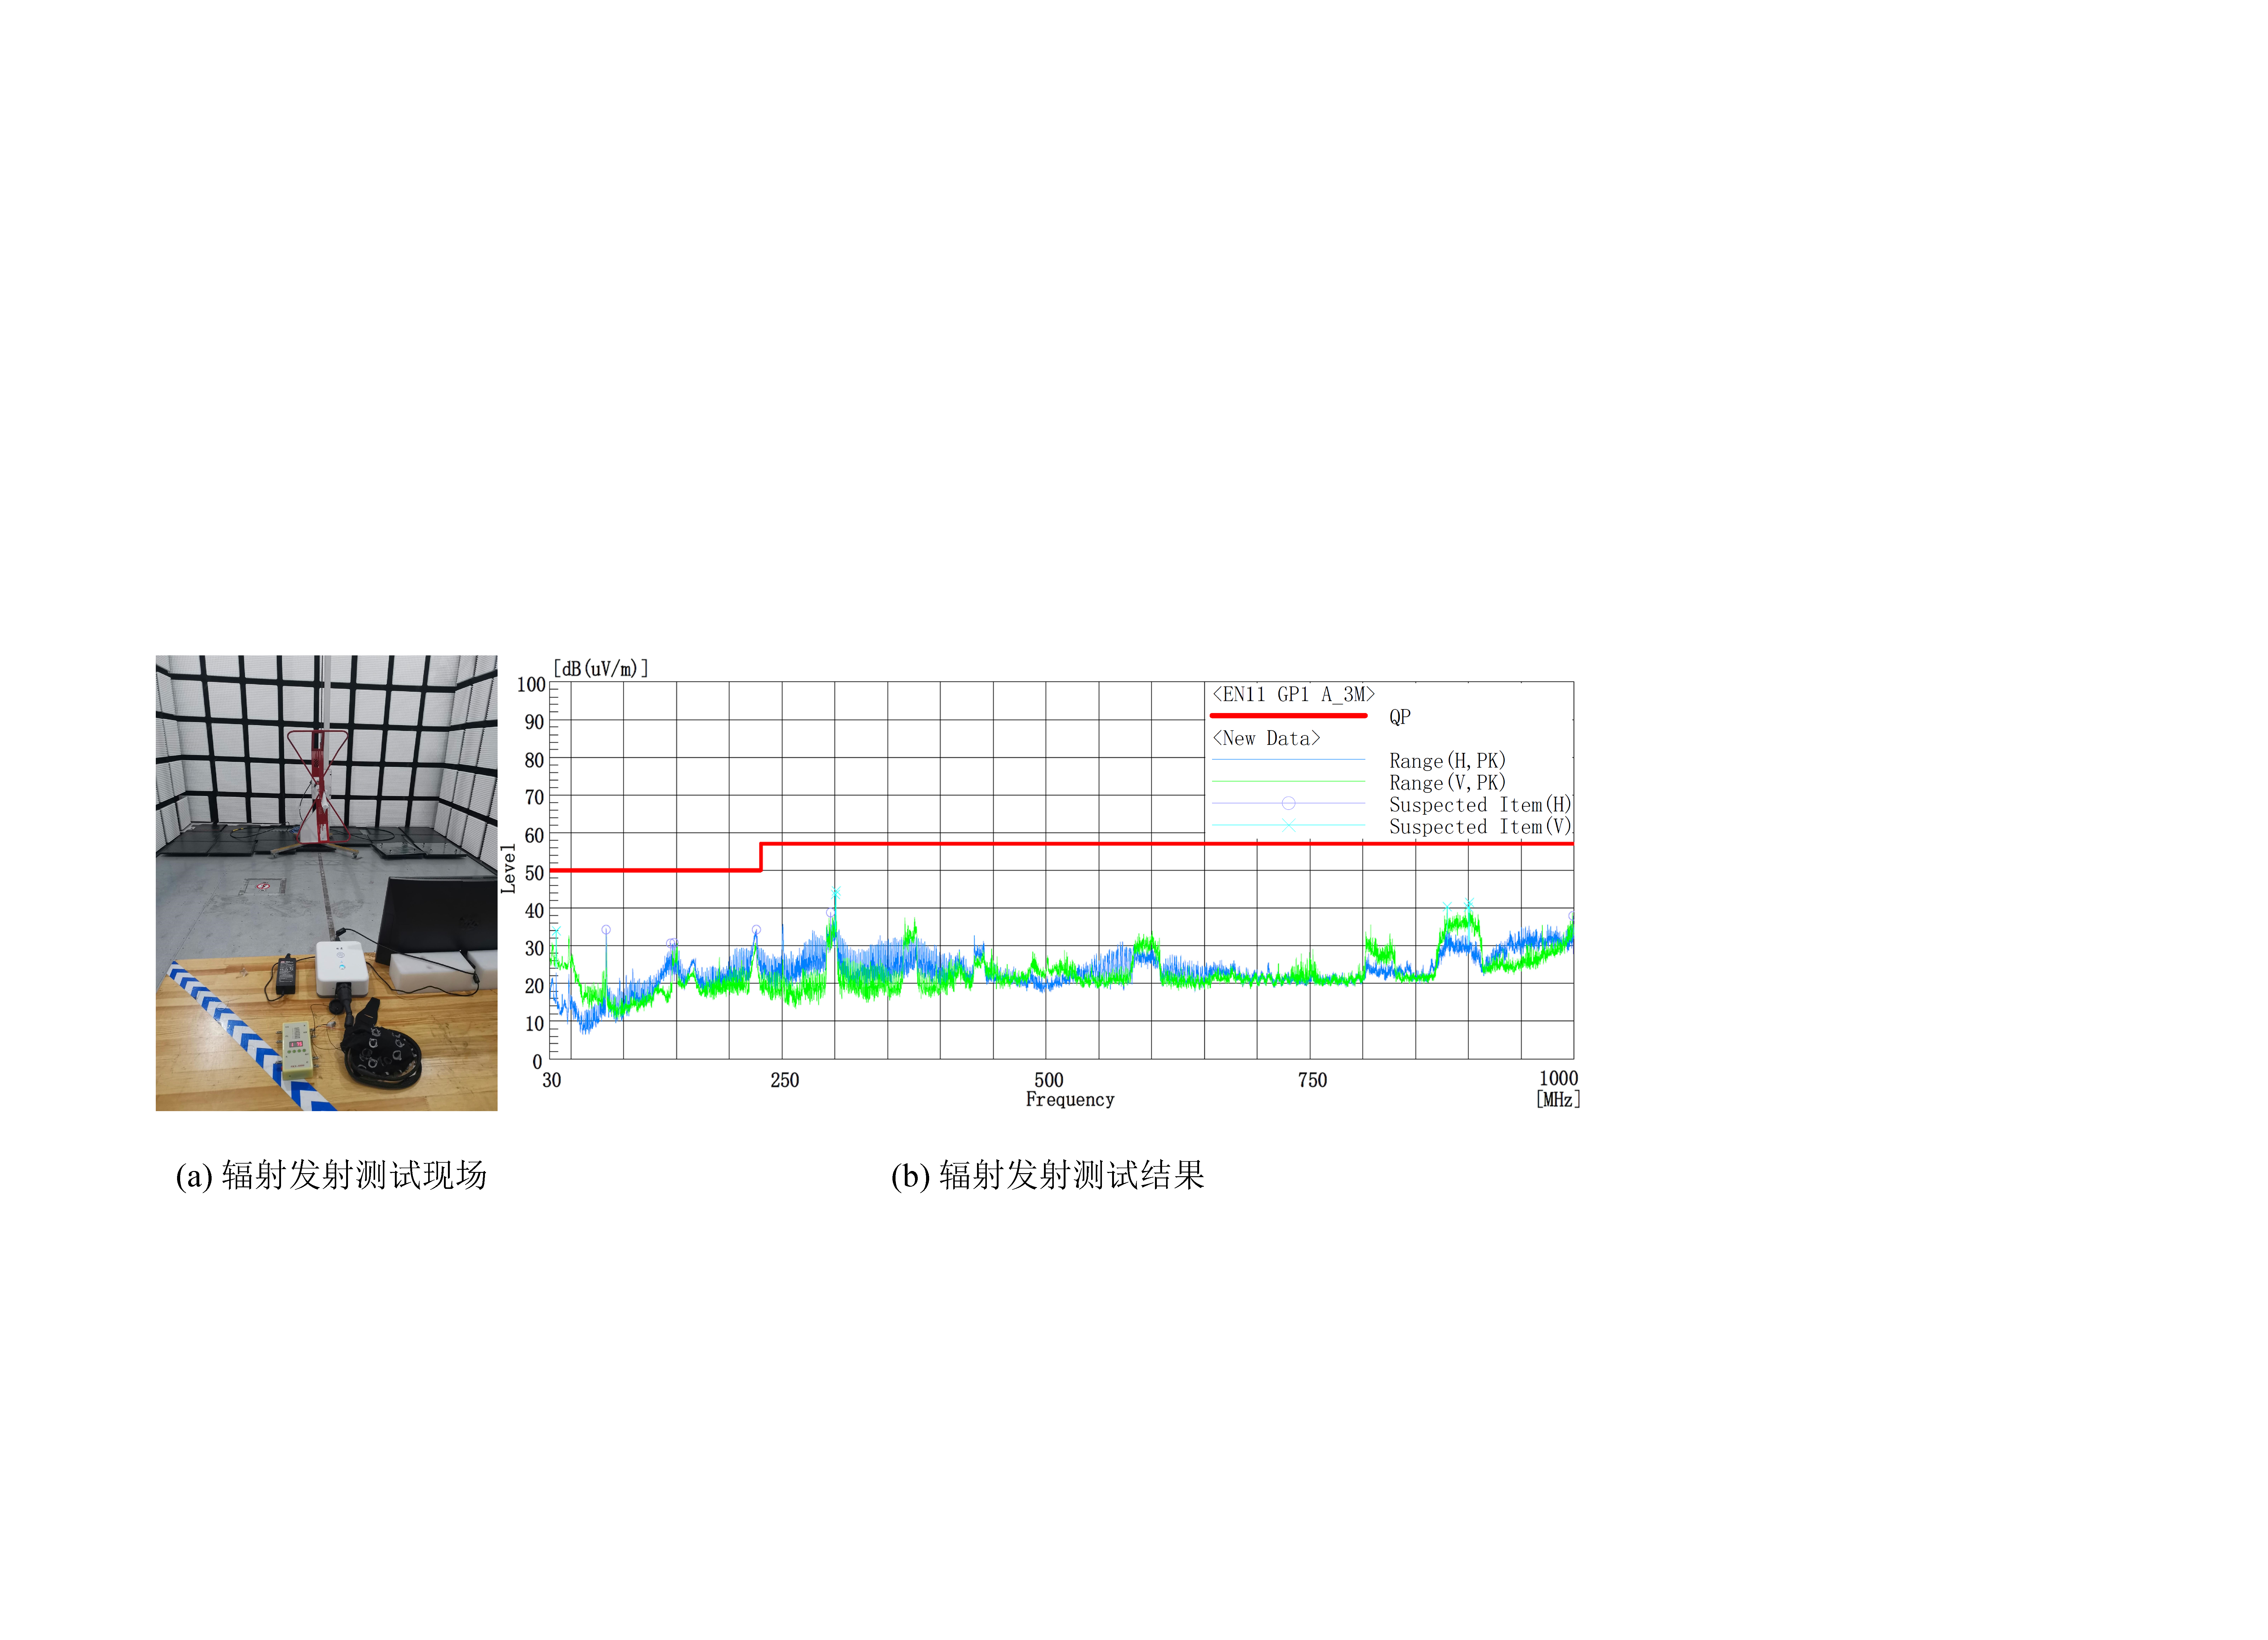
\includegraphics[width=0.60\textheight]{re_3.pdf}
	\caption{辐射发射测试现场与测试结果} 
	\label{fig2-26}
\end{figure}

辐射发射测试检测了JS-AINS-40系统在30 MHz-100 MHz频段内对外界的辐射干扰强度,检测现场及结果如图\ref{fig2-26}。图\ref{fig2-26}(b)中的红线代表国标设定的最大辐射干扰强度,可以看到,JS-AINS-40系统远低于这一指标,符合医疗电气设备的EMC要求。


\section{本章小结}
本章引入了自主设计的40导联EEG采集系统——JS-AINS-40,并以此为核心展开了详细介绍。首先,本章阐述了EEG信号的主要特点,并说明了针对这些特点,EEG采集设备应当具有的具体性能指标。紧接着,本章介绍了JS-AINS-40系统的整体框架——上位机、受试者和采集模块。其中作为核心的采集模块内部包含:虚拟串口通讯模块、数字电源模块、STM32H743IIT6主控模块、SPI隔离模块、电源隔离模块、ADS1299采集模块、模拟电源模块、采集前端与右腿驱动模块以及脑电极帽。考虑到实际使用时的安全性和可靠性,本章将上述子模块的电路集成在了脑电采集盒中,整个采集模块重量轻,体积较小,使用较为方便。接下来,本章说明了采集模块各子模块的器件选型以及配套电路,完成了对于JS-AINS-40系统硬件部分的介绍。

对于JS-AINS-40系统的软件部分,本章围绕下位机软件设计和上位机软件设计分别展开。其中下位机软件配合采集模块的硬件进行设计,使用STM32H743IIT6单片机控制ADS1299采集芯片,实现原始EEG数据的采集,并将其发送给上位机。上位机软件通过虚拟串口与下位机进行通信,并将接收的原始EEG数据进行存储与可视化。

最后,对JS-AINS-40系统的性能进行了测试与分析,从电压测量、共模抑制、噪声电平和EMC测试的结果可以看出,JS-AINS-40系统符合国标的相关要求,能够胜任EEG采集任务。接下来的章节,将使用JS-AINS-40系统采集相关EEG数据,并利用所提出的辨识算法对其进行分析。






\clearpage{\pagestyle{empty}\cleardoublepage}
% !Mode:: "TeX:UTF-8"

\chapter{基于梯度自动优化的脑电辨识模型}
情绪和疲劳状态在人的日常生活中扮演着重要的角色。前者能够对人的身心健康和工作效率等产生极大的影响,后者则可能对社会安全产生严重危害。EEG信号作为一种数据载体,可以包含人脑在不同状态下的大量信息,是广泛使用的评估人类心理、生理状态的指标之一。利用EEG信号进行的情绪和疲劳状态辨识,能够有效协助心理健康治疗以及工作疲劳预警。在各种分析方法中,深度学习,尤其是卷积神经网络,作为一种有效提取EEG信号特征的方法,在近年来取得了显著的成果。

虽然深度学习具有自动提取特征和有效分类的优点,但它也面临着网络结构设计困难,需要大量先验知识的问题。自动设计网络结构可以大幅节省专家的时间,因此,神经架构搜索技术应运而生。在本文中,针对EEG信号的时频域特点,对现有基于梯度的NAS算法——PC-DARTS\cite{3-7}进行了针对性的结构改进和优化。

具体来说:(1) 本节在人工设计的针对EEG的高性能网络架构的基础上,设计了一个新颖的CNN架构搜索空间,应用于基于EEG的大脑状态辨识任务。该搜索空间针对EEG特性设计,搜索过程无需从头开始,有效降低了搜索的时间复杂度。(2) 针对EEG通道之间的位置特征,EEG的频域特征以及各个通道的时域特征,提出了双流搜索框架,以提高网络的识别精度。(3) 在PC-DARTS的基础上,设计了自适应算法和早停算法,根据网络拟合情况自动调整模型的复杂度。使得NAS技术在EEG场景中的有效推广成为可能。

本章共引入三个数据集,将所提出架构应用于基于EEG的情绪识别和疲劳驾驶评估任务中。三个数据集包括公开的情绪辨识数据集、公开的疲劳驾驶数据集,以及一组由JS-AINS-40系统采集得到的情绪辨识数据集。结果表明,与现有的方法相比,本文得到的模型架构在这两项任务中都能达到具有竞争力的结果。这一结果不仅验证了所提出算法的性能,还证明了JS-AINS-40系统的可靠性。

\section{基于梯度自动优化的脑电辨识模型}
本节主要从针对不同类型EEG信号的特征提取、所设计算法的基础模型架构以及算法的具体优化框架三个方面展开,对所提出的EEG辨识模型进行了详细描述。
\subsection{特征提取}
EEG是对大脑皮层不同空间位置的测量,它包含多个时间序列。已有工作发现\cite{3-1},EEG信号不仅在频域有很大的差异,还具有明显的空间特征。因此,分析过程可以同时从频域、时域和电极的空间位置开始。为了证明上述特点,进一步对EEG信号进行以下处理。

(1) 差分熵

在深度学习技术出现之前,差分熵(Differential Entropy,DE)是常用于EEG辨识的人工特征\cite{3-2}。基于DE的方法在情感识别任务中取得了显著的效果,被证明是该领域中最有效的人工特征。对一段遵循高斯分布$N\left(\mu, \sigma^2\right)$的时间序列$X$,其DE的计算流程可以如下表述:
\vspace{3mm}
\begin{equation}
\begin{split}
    \label{deqn_ex3_1}
	h(X) &= -\int_{-\infty}^{\infty} \frac{1}{\sqrt{2 \pi \sigma^2}} e^{-\frac{(x-\mu)^2}{2 \sigma^2}} \log \left(\frac{1}{\sqrt{2 \pi \sigma^2}} e^{-\frac{(x-\mu)^2}{2 \sigma^2}}\right) d x\\
    &= \frac{1}{2} \log \left(2 \pi e \sigma^2\right)
\end{split}
\end{equation}
其中$\mu$,$\sigma^2$分别代表高斯分布的均值和方差,$e$为自然常数。

(2) EEG图像

将EEG信号转化为含有空间信息的图像是EEG分析领域的一种常见方法\cite{3-3}。对相应类型的EEG时间序列分别提取其DE特征(情绪EEG数据),进行快速傅里叶变换(Fast Fourier Transform,FFT)(疲劳EEG数据)来提取其频域特征。鉴于DE特征和EEG单一频段内的对数功率谱密度具有等同性\cite{3-10},以及它们在情绪识别和疲劳辨识领域的有效性\cite{3-2,3-30},本章将分别根据DE特征值和FFT的结果生成EEG图像,其具体步骤如下。

首先,为了保留头皮上EEG电极的三维空间分布信息,使用方位等距投影(Azimuthal Equidistant Projection,AEP)\cite{3-4}将电极的三维坐标投影到二维平面。这种方法有效地保留了电极之间的相对位置信息。

其次,应用Clough-Tocher算法\cite{3-5}对每个电极不同频段的DE值或FFT结果,根据二维电极坐标进行插值,并根据电极的数量生成适当大小的图像。在本文中,情绪EEG图像的大小被设定为64×64(公开的情绪辨识数据集)或48×48(JS-AINS-40系统采集得到的情绪辨识数据集),疲劳EEG图像的大小被设定为32×32。

最后,根据不同类型EEG信号的不同特点,对每个包含关键信息的频段都重复这一过程。对于具有$F$个频段的特定EEG信号,这种方法将产生$F$个不同的EEG地形图。$F$个EEG地形图将被合并,形成一个具有$F$通道的图像,作为模型输入的一部分。

\subsection{基础模型架构}
受试者的EEG时间序列将同时在时域和频域中被分割,以作为模型的输入。输入的每个样本由频域的EEG地形图$I$和时域的EEG时间序列$S$共同组成,其中$I \in R^{E \times E}$并且$S \in R^{C \times T}$。$E$代表像素数目,$C$代表EEG电极数,$T$代表每段EEG信号的采样点。在已有研究的基础上\cite{3-6},本章提出双流神经网络作为网络结构搜索的基础框架。双流意味着网络模型由两个具有不同输入模式的分支组成,并且两个分支通过各自相应的候选操作进行针对性构建。本模型的两个分支因其各自的特点被命名为频域流和时域流。图\ref{fig3-1}展示了该网络的框架。

\begin{figure}[!h]
	\centering
	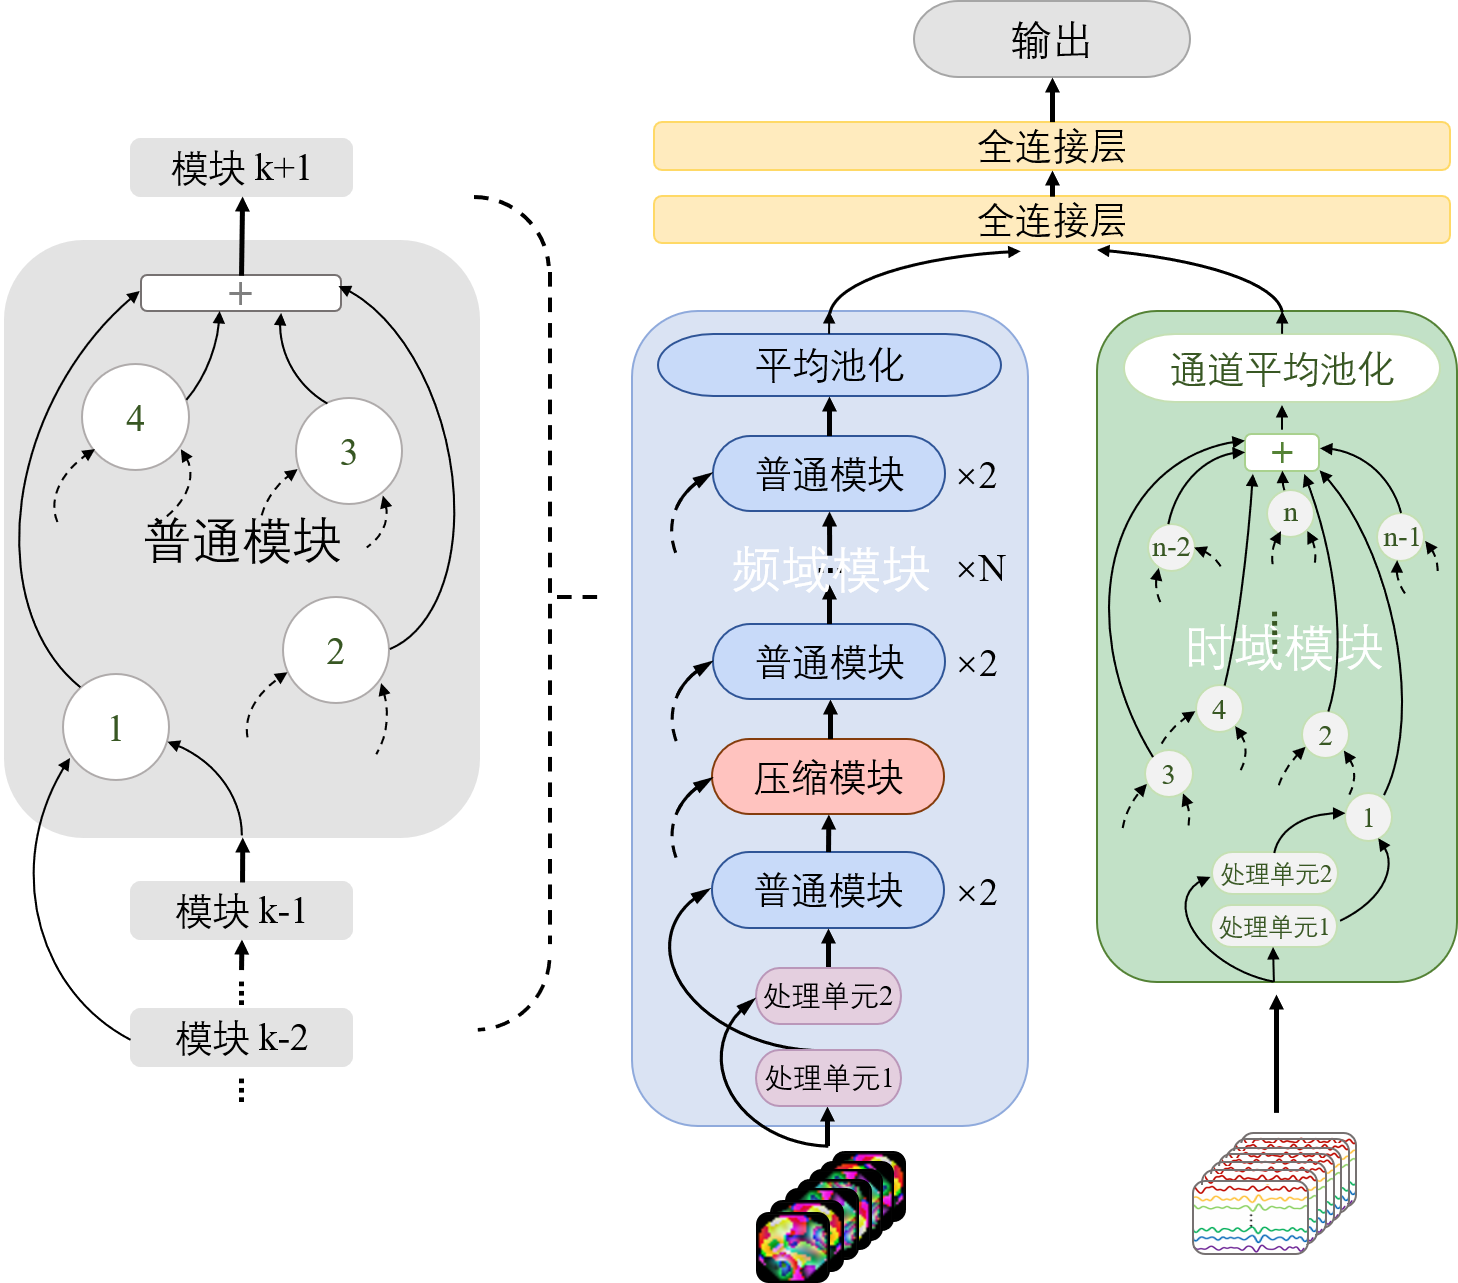
\includegraphics[width=0.55\textheight]{主模型图1.png}
	\caption{双流神经网络框架结构} 
	\label{fig3-1}
\end{figure}

(1) 频域流

将EEG信号转化为图像的相关研究\cite{3-3}验证了电极间相对位置这一信息的重要性,它同时也证明了通道间卷积对EEG特征提取的有效性。借鉴这一领域的先验知识,设计网络框架中的频域流。频域流将EEG图像作为输入,并使用图像识别中常用的扩张卷积(Dilated Convolution)、可分离卷积(Separable Convolution)、最大池化(Maximum Pooling)和平均池化(Average Pooling)作为候选操作来提取EEG图像的空间和频率特征。在图\ref{fig3-1}的左侧是频域流的具体结构和内部连接,以及频域流内部普通模块的结构。频域流的设计继承自PC-DARTS,其框架结构由普通模块和压缩模块堆叠而成。普通模块与压缩模块的内部结构相同,但后者通过引入步长(Stride)为2的候选操作,实现了对特征图大小的压缩(压缩模块的原理在3.1.3优化框架一节中详细介绍)。压缩模块的存在保证了模型能够在深度增大时,时刻保持压缩特征,扩张感受野以及提取全局特征的能力,为模型架构的变化提供性能支撑。EEG图像输入时,频域流首先使用处理单元1与处理单元2对输入的EEG图像进行3×3卷积运算,形成第一个普通模块的两个输入。普通模块内部节点上的虚线代表两个候选操作。频域流中$N$被设置为4。

(2) 时域流

已有研究\cite{3-8}引入了一个名为巧合筛分卷积神经网络(Coincidence-Filtering-based CNN,CF-CNN)的模型,它只对EEG信号的每个通道进行两次时间卷积(Temporal Convolution)和一次通道平均池化(Channel Average Pooling)。该模型有效地利用了巧合筛分的思想,成功地提取了EEG信号的时间依赖性以及EEG电极通道的具体特征。它的优越性已经在疲劳判别和情绪识别数据集中得到了证明。在CF-CNN模型的基础上,选择时间卷积和通道平均池化操作来提取与通道相关的特征,完成时域流的构建。在图\ref{fig3-1}的右侧,展示了时域流的独特结构以及它所包含的时域模块的内部连接方式。时域流包含一个时域模块,时域模块内部首先通过两个处理单元对输入的时域信号进行1×1卷积运算,为第一个节点生成两个输入。连接到内部节点的虚线也代表两个任意的候选操作。在本章中,时域模块内部的$n$被设定为11。

在网络的最后,两个流的输出通过两个全连接层结合起来,完成EEG信号的识别。然而,上述模型的有效性高度依赖于架构设计和超参数选择。因此,引入网络结构搜索算法,在一个广阔的搜索空间上进行结构搭建,以寻找EEG信号的特定模式。

\subsection{优化框架}
为了以最小的计算资源消耗快速演化网络结构,使用基于梯度的网络结构搜索算法作为参考。其中PC-DARTS作为这一领域中的经典框架,在对CIFAR-10数据集的图像进行分类时,成功的将模型架构搜索时间减少到了2.4小时以内。因此,本章的研究将以该方法为基础进行展开。

(1) 网络结构搜索空间

PC-DARTS的多分支结构有助于建立复杂的网络框架,并在图像识别任务中取得了瞩目的成果。因此,本章将在模型中保留这一结构,并将其应用于基于EEG的模型结构搜索中。本节在3.1.2节基础模型架构的基础上,为两个流建立不同的搜索空间。整体来看,模型的搜索空间中包含有三种不同的模块(普通模块、压缩模块和时域模块)。

在频域流中,由于模型的输入是EEG图像,其数据结构与RGB图像相似,因此本章保留了PC-DARTS中的所有原有候选操作,并在此基础上搜索最适用于该流的模块结构,其中包括3×3大小的最大池化、3×3大小的平均池化、3×3大小、5×5大小的可分离卷积、3×3大小、5×5大小的扩张卷积、直接连接以及无连接。所有卷积操作的卷积核数量被设定为16。

在普通模块和压缩模块内部,设置了四个节点(不包括两个输入节点和一个输出节点)。节点的概念继承自PC-DARTS,它本质上代表了对网络中的张量的连接操作。这些张量来自前位的节点或模块,它们的输出经过一组特定的操作后到达当前节点。节点这一特殊概念的引入有利于网络结构的设计和变更。每个节点只可以接收其前向方向上任意两个节点(或者模块)的输出。模块内所有节点的输出将被串联成为模块的输出。

从普通模块和压缩模块外部来看,根据已有研究中的模型规模\cite{3-3},频域流中堆积的模块的初始个数被设置为11。堆积模块的策略也将遵循PC-DARTS的设计——网络由两个普通模块与一个压缩模块交替构建。压缩模块是一个特殊的模块,其引入的目的是减小通过网络的特征图的大小。为了达到这个目的,与压缩模块的输入节点相邻的所有节点上的候选操作都将被设置步长为2。每个模块将前面两个模块的输出作为输入。频域流的最终输出将通过一个平均池化层传递给全连接层。在搜索过程中,模型将不断调整频域流内的模块堆叠数量,而频域流模块内部的节点数量将一直保持不变。

在时域流中,参考CF-CNN的设计,将网络构建为只包含一个模块(时域模块)的结构。最初,时域模块将包含11个内部节点(不包括两个输入节点和一个通道平均池化节点)。在这11个节点之间,有1×1、1×3、1×5、1×7、1×9、1×11大小的时域卷积、直接连接和无连接作为候选操作。所有卷积操作的卷积核个数被设定为32。这些操作确保了时域流将优先提取与通道相关的时间信息。与频域流一样,每个节点可以从其前向方向上的任意两个节点处接收输出。在搜索过程中,模型将不断调整时域流内的节点数量,而时域模块的数量将一直保持不变。

(2) PC-DARTS在EEG上的改进

当模型规模设置过大或训练集容量过小时,PC-DARTS在网络结构搜索过程中会随着训练迭代次数的增加而更易倾向于选择弱参数操作(如直接连接、最大池化等),造成网络结构的崩塌现象\cite{3-9}。这种现象产生的根源在于网络中不同模块的前后堆叠。网络输入端的模块接触到的是最纯净的信息,而整个网络后端的模块接触到的是已经提取过的抽象特征(随着网络结构的加深,这个问题将愈加明显),因此后端的模块将倾向于直接传递抽象特征,即使用直接连接操作,以获得更好的分辨能力。由于模型内部的同种模块之间结构共享,这一问题将会扩散至整个网络,使得模型最终发生崩塌。

同时,由于PC-DARTS以与网络权重相同的方式将操作权重转换为可微调的对象,并将架构搜索过程转换为双层优化问题:
\begin{equation}
\label{deqn_ex32}
\begin{array}{cl}\min _\alpha & \mathcal{L}_{\text {val }}\left(w^*(\alpha), \alpha\right) \\ 
\text { s.t. } & w^*(\alpha)=\operatorname{argmin}_w \mathcal{L}_{\text {train }}(w, \alpha)\end{array}
\end{equation}
这使得网络权重和操作权重的优化形成一个竞争过程。网络权重$w$因为具有更多的可学习参数,对交替训练过程中损失的变化相对鲁棒,因此在竞争中对操作权重$\alpha$具有一定的优势。$\alpha$为了在竞争中获得胜利,将会变得更倾向于选择弱参数操作,这增大了模型崩塌的概率。

此外,PC-DARTS为减少性能消耗,使用了部分通道连接(Partial-Channel-Connections)的方法:
\begin{equation}
    \label{deqn_ex33}
f_{i, j}^{\mathrm{PC}}\left(\mathbf{x}_i ; \mathbf{S}_{i, j}\right)= \sum_{o \in \mathcal{O}} \frac{\exp \left\{\alpha_{i, j}^0\right\}}{\sum_{o^{\prime} \in \mathcal{O}} \exp \left\{\alpha_{i, j}^{o^{\prime}}\right\}} \cdot o\left(\mathbf{S}_{i, j} * \mathbf{x}_i\right)+\left(1-\mathbf{S}_{i, j}\right)^* \mathbf{x}_i
\end{equation}
其中$\mathbf{S}_{i, j}$代表了随机采样掩码。这一方法使得每次网络结构更新时,只有少数通道被更新,而其余部分保持不变。这进一步促使网络选择弱参数操作,加剧了网络结构崩塌的风险。尽管PC-DARTS设计了边缘正则化方法:
\begin{equation}
    \label{deqn_ex34}
\mathbf{x}_j^{\mathrm{PC}}=\sum_{i<j} \frac{\exp \left\{\beta_{i, j}\right\}}{\sum_{i<j} \exp \left\{\beta_{i, j}\right\}} \cdot f_{i, j}\left(\mathbf{x}_i\right)
\end{equation}
为每一个模块中节点的输入引入了一个参数$\beta$,$\beta_{i, j}$代表了节点$i$,$j$之间的边缘正则化权重,能够一定程度上减弱上述影响。

但边缘正则化的存在有时并不能保证网络的最终搜索结果不会崩塌(特别是在数据量较少的EEG数据集上)。因此,本章在训练过程中引入了层数自适应机制和早停机制:
在NAS搜索过程完成后,如果模块内被选为直接连接的边数达到25\%,则认为搜索已经崩塌,网络将自动降低模型复杂度——减少堆叠模块的数量(针对频域流)或模块内的节点数量(针对时域流),开始新一轮搜索。如果在停止训练时,模型的训练精度仍然不能稳定在85\%以上,那么认为应该增加模型的复杂度(增加堆叠模块的数量或模块内的节点数量)。

在NAS过程中,当操作权重$\alpha$在一段时间内(一定数量的epochs,在本章中设置为10)保持稳定时,就可以停止NAS进程。


\section{实验描述}
在本章中,基于EEG的情绪辨识公开数据集、疲劳驾驶检测公开数据集以及JS-AINS-40采集的情绪辨识数据集将被分别使用,验证所提出模型的有效性。
\subsection{情绪辨识公开数据集}
(1) 数据集描述

在情感识别领域,上海交通大学的情感数据集(SEED)在众多研究中被广泛使用\cite{3-2}。SEED数据集包含了15个受试者(Subject)的EEG信号,这些信号是通过观看15个情绪电影片段收集的。其中有三种类型的情绪,包括高兴、中性和悲伤,每个电影片段大约持续4分钟。每名被试总共包含三个时段(Session),每个时段中均进行15次观影试验。受试者的EEG信号由62个脑电极以1000 Hz的采样率完成记录,这些信号用0 Hz-75 Hz的带通滤波器进行了预处理。之后,采集者将数据降采样至200 Hz。在此基础上,本章将EEG信号沿时间方向划分为一系列不重叠的1秒数据段。此外,挑选了十二个电极的EEG信号作为时域流的输入,即FT7、FT8、T7、T8、C5、C6、TP7、TP8、CP5、CP6、P7和P8,因为研究表明它们在情绪识别中起着重要作用\cite{3-11}。

同时,SEED中所有62个通道的数据被用作频域流的输入,以保留EEG电极之间的空间位置信息。数据DE特征的提取已经在SEED数据集中完成,本章分别提取每个1秒数据段对应的DE特征作为频域流的输入。对于每个1秒数据段,首先使用零填充(Zero Padding)将DE特征扩展到64个通道,之后对其进行归一化处理,即每个被试的数据将减去其平均值并除以其标准差。然后,DE特征的五个频段:$\delta$频段、$\theta$频段、$\alpha$频段、$\beta$频段和$\gamma$频段将被分别转换为相应的EEG图像,将其合并即获得频域流的五通道EEG图像输入。由于不同情绪视频的长度不一致,捕获的情绪EEG信号的长度也不一样。为了保证不同类别数据量的平衡性以及情绪唤醒的有效性,统一选择每段数据的最后185秒和其对应的DE特征作为模型的输入。

(2) 分类模型以及性能度量

为了评估所提出框架的跨被试情绪分类性能,采用留一法(Leave-One-Subject-Out,LOSO)进行验证实验。在本章情况下,这种方法的核心是将测试被试的所有数据从训练数据中剔除,以验证模型是否提取到了关于情绪的通用性特征\cite{3-13}。在每次LOSO实验中,将选择一名被试者的数据作为测试数据,其余被试者的数据被用作训练数据。这个过程将自动重复,直到每名受试者的数据都作为测试集被模型验证过一次。

根据分类结果,本章引入了一些常用的分类指标来评估网络模型的整体性能,包括精度(Precision,PR)、F1分数(F1-score,F1)\cite{3-14}、宏观平均F1分数(Macro-averaging F1-score,MF1)、准确率(Accuracy,ACC)以及来自所有情感类别的接收者操作特征(Receiver-Operating-Characteristic,ROC)曲线的平均曲线下面积(Area Under the Curve,AUC)。这些指标的计算公式如下:

\begin{equation}
    \label{deqn_ex35}
T P R_i=\frac{T P_i}{T P_i+F P_i}
\end{equation}

\begin{equation}
    \label{deqn_ex36}
R E_i=\frac{T P_i}{T P_i+F N_i}
\end{equation}

\begin{equation}
    \label{deqn_ex37}
F 1_i=\frac{2 P R_i \times R E_i}{P R_i+R E_i}
\end{equation}

\begin{equation}
    \label{deqn_ex38}
M F 1=\frac{\sum_i^C F 1_i}{C}
\end{equation}

\begin{equation}
    \label{deqn_ex39}
A C C=\frac{\sum_i^C T P_i}{N}
\end{equation}

\begin{equation}
    \label{deqn_ex310}
A U C=\frac{1}{C_C^2} \times \sum_{\substack{1 \leq j<C-1 \\ 2<k \leq C j<k}}\left[\frac{\sum_l^{N_j+N_k}\left(S_p>S_n\right)+0.5 \times \sum_l^{N_j+N_l}\left(S_p=S_n\right)}{\left(N_{j P}+N_{k P}\right) \times\left(N_{j N}+N_{k N}\right)}\right]
\end{equation}

\vspace{5mm}


其中$T P_i$是类别$i$中真正例样本的个数(True Positive Samples),$F P_i$是类别$i$中假正例样本的个数(False Positive Samples),$F N_i$是类别$i$中假负例样本的个数(False Negative Samples),$C$代表了样本类别数,$N$是测试样本总数,$N_i$是类别$i$中的样本个数,$N_{i P} / N_{i N}$是类别$i$中的正例与负例样本数之比,$S_p$与$S_n$是类别$j$和$k$组成的集合的Wilcoxon-Mann-Witney测试\cite{3-15}分数。

(3) 训练参数

本章模型将SGD优化器与学习率余弦退火算法结合使用,在网络结构搜索阶段最小化模型损失。由于较大的学习率有助于双层优化过程找到更好的架构,因此SGD优化器中参数设置为:学习率0.1、动量0.9、权重衰减0.0003以及batch size 64。搜索过程中dropout概率保持为0.3。根据双层优化过程的性质,将操作权重的学习率设置为0.0006,操作权重衰减率设置为0.001。

训练集数据将被随机分为两个大小相同的子集,分别用于网络权重优化和操作权重优化。由于网络模型在搜索过程中同时优化了超网络中所有候选操作的权重,最终的最优架构不一定具备当前数据的最佳网络权重,因此需要对最优架构进行再训练。

在再训练阶段,利用Adam优化器将网络的损失降到最低。此时学习率被设置为0.02,动量被设置为0.9,权重衰减被设置为0.0012,batch size被设置为64,dropout概率被设置为0.4。再训练阶段无需进行网络结构变动,只需对网络权重进行调整,因此使用较小的学习率寻找权重最优值。

\subsection{疲劳驾驶检测公开数据集}

(1) 数据集描述

本文使用的疲劳驾驶检测公开数据集为Cao等人采集的数据集\cite{3-16}。该数据集收集了27名22-28岁的志愿者的EEG数据。实验使用了32通道的有线脑电极帽来记录EEG信号,其中包括30个EEG电极和2个参考电极。采集时,EEG信号被放大并以500 Hz的采样率进行数字化(在使用中本章进一步将数据降采样至250 Hz)。所有的EEG信号都使用了带通滤波器(1 Hz-50 Hz的有限脉冲响应(Finite Impulse Response,FIR)滤波器)和伪影抑制(Artifact Rejection)来进行预处理。

本数据集的实验模拟了夜间四车道高速公路上的驾驶环境,要求受试者将汽车保持在车道中央巡航。该实验的设计是为了模拟一种非理想的道路状况,它将触发汽车以相等的概率向第三条车道的右侧或左侧进行漂移。每个车道偏离事件包括四个标记:基线期(Baseline Period)、漂移开始(Onset of Drift)、反应开始(Onset of Response)和事件结束(The End of Event)。偏移事件发生前所有30个通道的3秒EEG数据将被进行FFT变换,并提取其$\theta$频带、$\alpha$频带和$\beta$频带。这三个频段被分别插值为32×32大小的图片后,共同构成EEG图像,并作为频域流的输入。


此外,本文只使用Fcz、Tp7、Cp3和Oz通道的EEG时间数据作为时域流的输入,因为研究发现这四个通道在检测驾驶员疲劳方面有着重要作用\cite{3-17}。与上一节一样,每名受试者的数据都进行了归一化操作。

(2) 标签获取

由于原始数据没有提供标签来确定每段EEG是否处于疲劳状态,因此需要进行人工标注。

受试者的反应时间(Response Time,RT)在本章被提取出来作为衡量受试者是否处于疲劳状态的指标。RT是指在模拟驾驶过程中发生汽车漂移与受试者做出纠正反应之间的时间间隔。首先,从当前事件中提取的反应时间被称为局部RT,它代表受试者的短期疲劳状态。在当前事件之前的90秒内所有事件的平均反应时间被称为全局RT,代表受试者的长期疲劳状态。将在整个90分钟的实验中获得的所有局部RT从小到大进行排序,并将第$Z$个RT作为实验的警戒RT($Z$等于某个被试的样本总数乘以5\%),它代表受试者在实验期间清醒状态下的反应速度。当偏移事件的局部RT和全局RT都小于警戒RT的1.5倍时,认为此时被试是清醒的;当偏移事件的局部RT和全局RT都大于警戒RT的2.5倍时,认为被试此时处于疲劳状态。介于两者之间的部分没有被分类,因为这可能归因于其他未知的过程,例如,受试者在进行思想游荡\cite{3-18}。
\newpage
(3) 训练参数

为了使每名受试者的疲劳和清醒事件保持平衡,本章删除了六个不符合条件的受试者。从数据集的角度来看,最终选择的21名受试者共包含11,772个不同类别EEG样本,其中疲劳状态的数量为6,054,清醒状态的数量为5,718,二者基本处于平衡状态。

同样,LOSO交叉验证法被用来验证模型的性能。引入的评价指标与之前的一致。模型架构搜索和再训练阶段的超参数与情感识别任务中的超参数相一致。




\subsection{JS-AINS-40系统情绪辨识数据集}
为验证JS-AINS-40的实际使用效果,设计相应的EEG情绪实验。本章使用JS-AINS-40系统和搭载配套上位机软件的计算机(带有音响)作为实验器材。
在本次实验中获得的数据集即JS-EM Dataset,实验的详细内容如下所述。

(1) 被试与实验内容

本次实验共选取了13名年龄在20-30岁之间受试者(8名男性,5名女性),这些受试者均身体健康,无视力、听觉障碍及大脑相关疾病。所有被试在实验开始前均进行了一段时间的情绪平复,以保证实验开始时情绪能够被正常唤起。同时,向所有受试者介绍了实验的具体流程,以保证实验的顺利进行。13名受试者中有5人从未参加过任何EEG实验,其他人则有过相关实验经历。本实验经过了天津医科大学总医院的伦理委员会的审查,并签署了知情同意书。

本章实验引入了三类不同电影的片段,分别对应高兴、悲伤与中性三种不同的感情。每段影片均经过精心挑选与编辑,能够创造连贯的情感,并可以最大程度唤起受试者的相应情绪。被试需要在相对独立,没有外部环境干扰的房间中独自观看影片,以保证EEG数据的有效性。具体内容如表\ref{tab3-1}所示。

\begin{table*}[!h]
\caption{电影片段具体信息}  \label{tab3-1}
\centering
\wuhao{
    \begin{threeparttable}
    \setlength{\tabcolsep}{5mm}{
        \begin{tabular}{cccc}
            \toprule
            编号 &电影片段来源 &情绪类型 &片段时常\\
            \midrule
            1   &武林外传        &高兴   &9分35秒\\
            2   &憨豆先生1       &高兴   &8分45秒\\
            3   &憨豆先生2       &高兴   &9分10秒\\
            4   &亲爱的          &悲伤   &8分30秒\\
            5   &七号房的礼物     &悲伤   &9分55秒\\
            6   &舐犊情深        &悲伤   &9分20秒\\
            7   &航拍中国(第一季) &中性   &9分40秒\\
            8   &航拍中国(第二季) &中性   &9分50秒\\
            9   &蓝色星球(第一季) &中性   &10分05秒\\
            \bottomrule
        \end{tabular}
        }
    \end{threeparttable}
    }
\end{table*}

每个片段播放结束后,被试都会获得一段情绪平复时间(时长因被试特点而进行调整),以保证每次实验开始时被试均处于中性状态。在情绪平复时间内,被试会被要求填写调查问卷,以获取被试对于实验设计的意见。

(2) 实验流程

实验过程中,屏幕上会全程提示受试者接下来将要进行的实验步骤,保证受试者不会受到外界干扰。实验的具体流程如下所示:1) 受试者稳定情绪,并了解实验相关流程,签署实验同意书;2) 准备阶段,屏幕上提示受试者保持专注,给与受试者十秒钟时间进入状态;3) 情绪唤起阶段,程序随机挑选三类影片中的一段进行播放;4) 情绪平复阶段,观影结束,受试者填写问卷,并平复情绪。
\begin{figure}[!h]
	\centering
	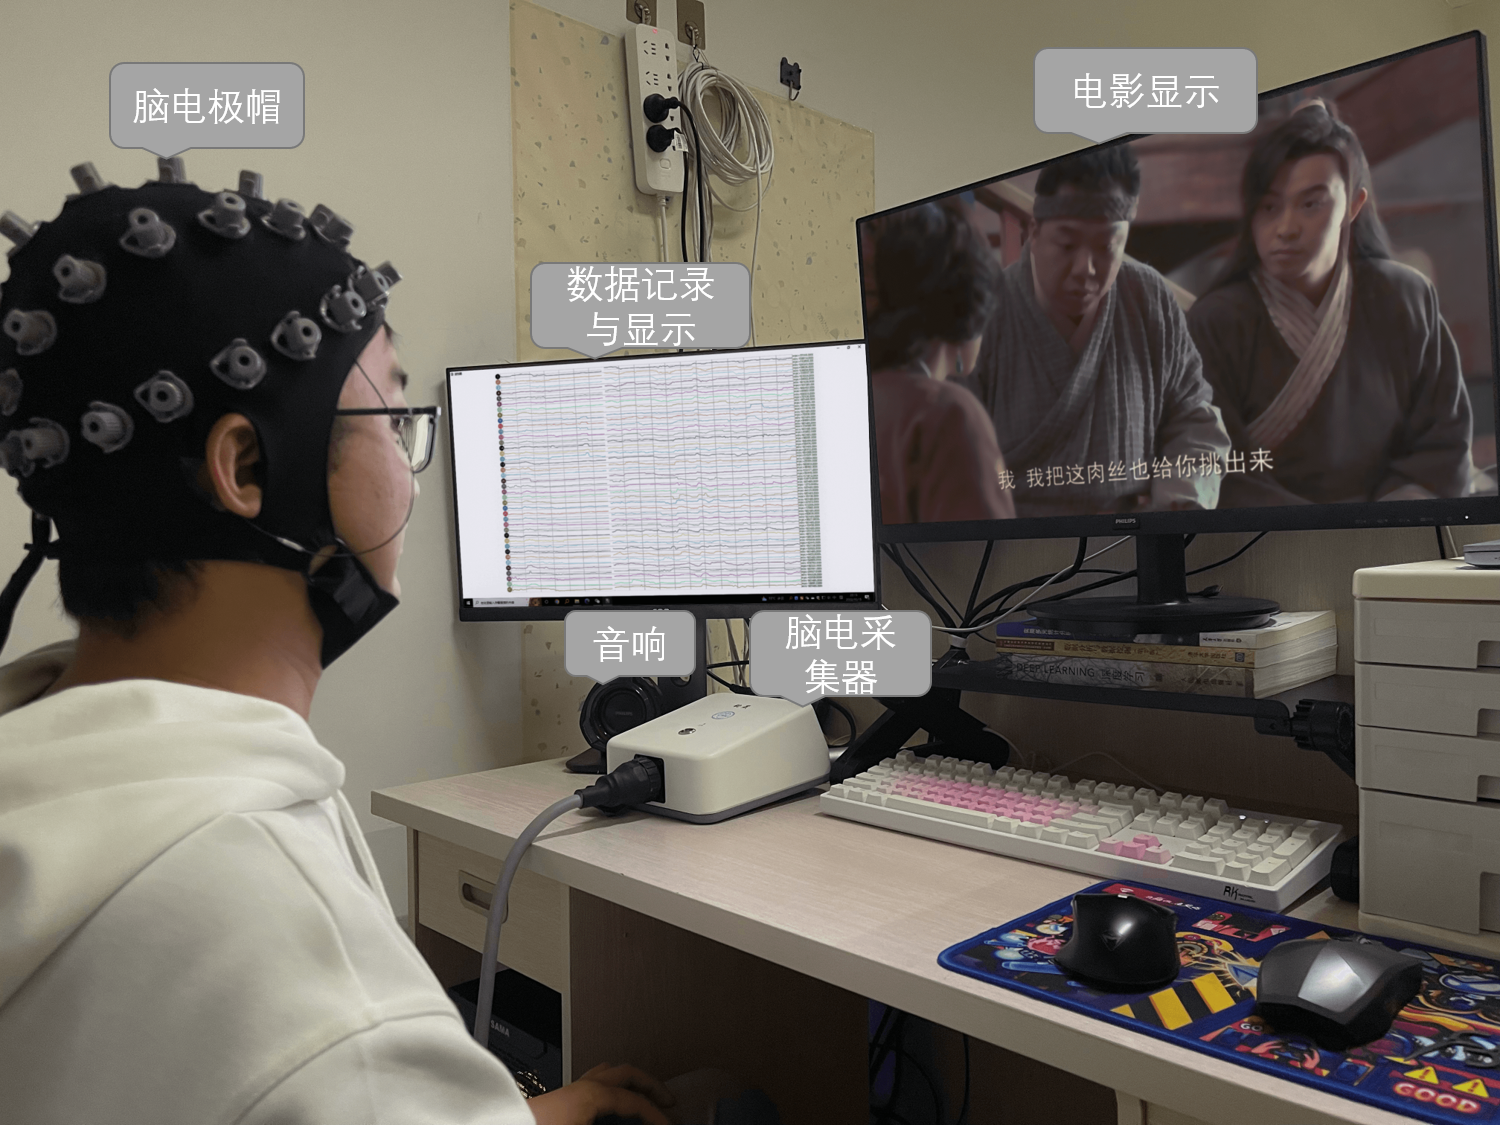
\includegraphics[width=0.44\textheight]{情绪实验.png}
	\caption{情绪实验场景图} 
	\label{fig3-2}
\end{figure}

当第一遍流程结束后,实验将会从阶段2) 准备阶段,重新开始,直至完成18次实验。18次实验中将会包含高兴、悲伤与中性三种电影片段各6次,其出现顺序由电脑随机决定。实验场景如图\ref{fig3-2}所示。

(3) 数据预处理

上述数据以1000 Hz的采样率在50 Hz工频陷波下进行采集。采集后,使用1 Hz-60 Hz的带通滤波器对数据进行滤波,以减小噪声干扰。为降低运算复杂度,将数据从1000 Hz降采样至250 Hz。此后,使用独立分量分析(Independent Component Analysis,ICA)\cite{4-29}来消除伪迹和眼电信号的干扰。

为了保证不同类别数据量的平衡性以及情绪唤醒的有效性,统一选择每段数据的最后360秒,并将其切片为1秒数据
段。全部40个通道的1秒时序信号将作为时域流的输入。对于频域流输入,首先提取1秒数据段的DE特征(频带与SEED中一致),并使用零填充将DE特征扩展到48个通道。之后对其进行归一化处理,即每个被试的数据将减去其平均值并除以其标准差。每个频带的DE特征将被插值为48×48大小的图片,合并后作为EEG图像输入频域流。

(4) 训练参数

LOSO交叉验证法被用来评估模型的性能,同时这里也引入了与之前数据集相同的评价指标。模型架构搜索和再训练阶段的超参数与SEED数据集所设置的超参数保持一致。

\section{结果与讨论}

从搜索中得到的模型结构完成再训练后,就可以被应用在测试数据集上检验模型性能。所有受试者的平均辨识准确率将作为模型性能的评判标准,并与其他基于脑电的辨识算法进行比较。当不同的被试作为测试集时,NAS算法将搜索得到不同的最优网络架构,带来高昂的时间开销。因此,在NAS进程中,只有少数受试者的数据被用作测试集,以获得一些最佳架构。随后,选择具有最佳泛化能力的架构进行再训练过程。

\subsection{情绪辨识公开数据集分类结果}

(1) 结构搜索进程

在NAS过程中,早停机制影响了模型搜索的最终结果。为了保证结果的可靠性,本节进行了多次NAS以获取直接连接在总操作中的平均比例。图\ref{fig3-3}(a)展示了堆叠不同数量的模块(频域流)和不同数量的内部节点(时域流)下模型内部直接连接操作的最终占比。可以看出,在频域流中的模块层数达到5之前,模型结构仍处于过拟合阶段。因为搜索结果中存在大量的直接连接操作,模块的内部结构仍然在趋于简化。同样,时域模块内部的节点数量被最终选定为7个。图\ref{fig3-4}展示了最终模型内部获得的三种模块,三种不同模块的内部连接结构和操作选择见表\ref{tab3-2}。如前文所述,每个压缩模块内与输入节点相邻的操作的Stride被设置为2,用红线加以表示。

为了验证早停算法的有效性,本节还比较了未进行再训练的模型堆叠不同数量的模块和内部节点时在测试集上的分类准确率,并增加了一些在搜索过程中没有出现过的架构以证明最终结果的合理性(由于在达到当前的最佳架构之前,训练集上的准确率几乎一直保持在较高值(过拟合现象明显)。在模型简化过程通过最佳点后,模型在训练集上的准确率也不会有大幅下降。因此,为了更直观地看到模型在测试集上的性能变化,没有在图\ref{fig3-3}(b)中绘制模型在训练集上的准确率曲线)。图\ref{fig3-3}(b)所示的结果表明,在目前的架构下,模型在验证集上达到了最高的分类精度,并且提出的早停机制能有效地获取最合理的模型复杂度。

\begin{figure}[!b]
	\centering
	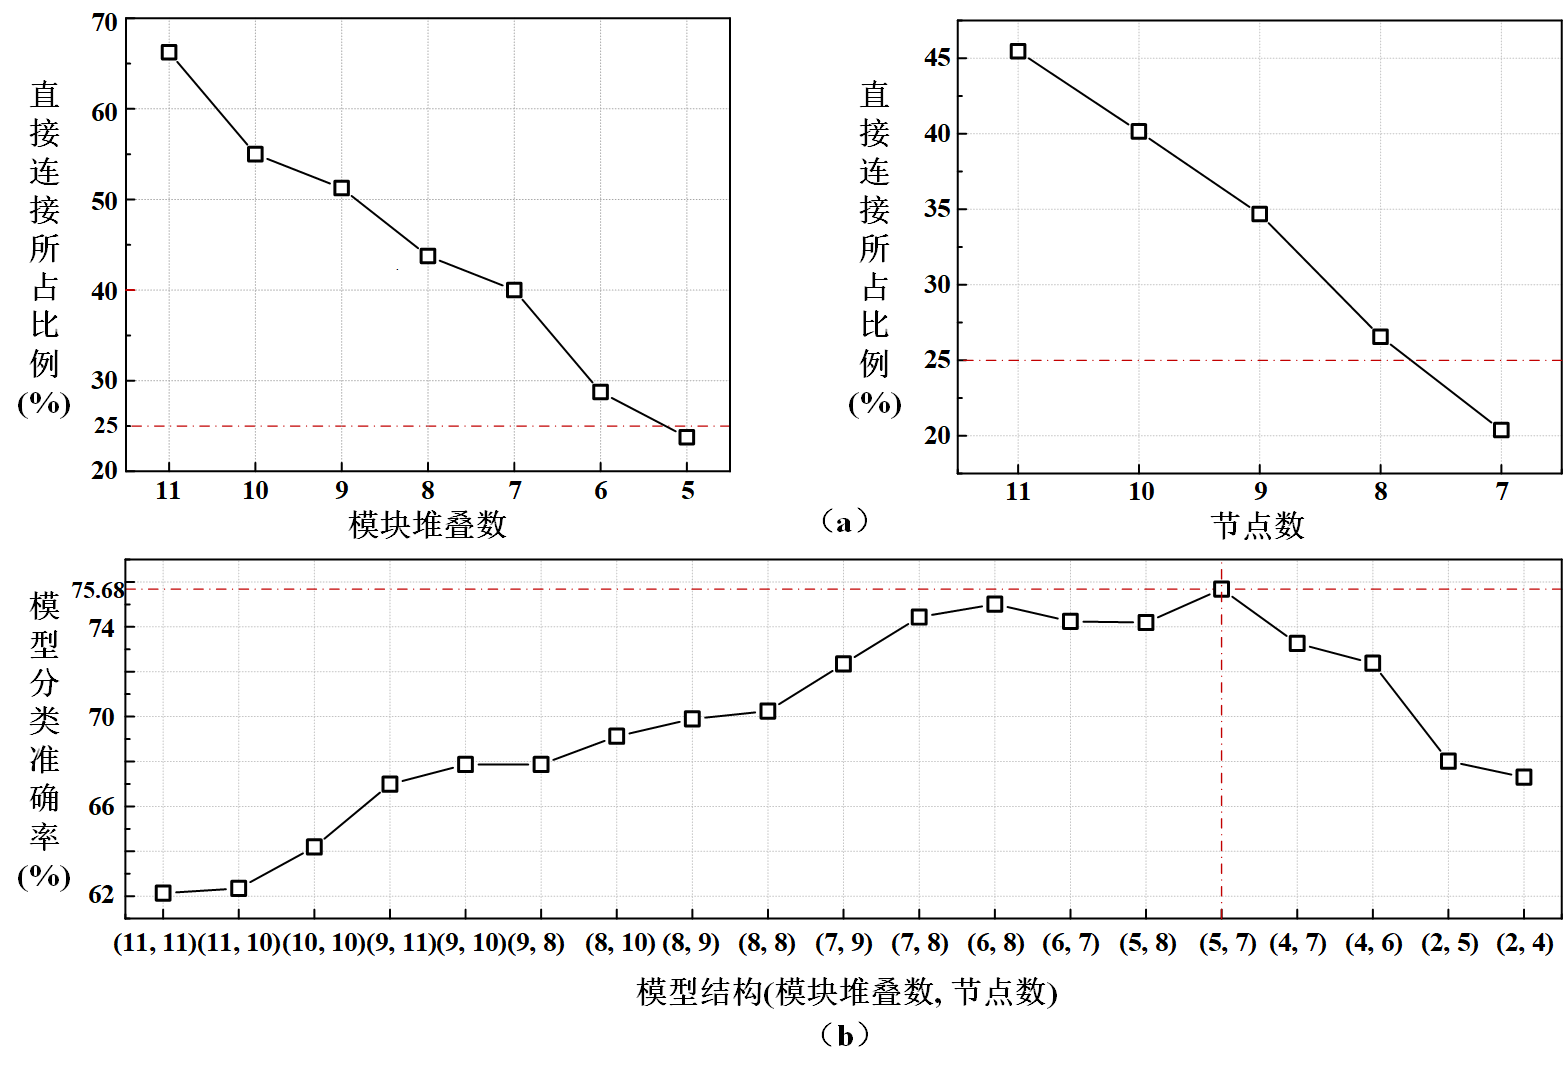
\includegraphics[width=0.60\textheight]{SEED消融.png}
	\caption{SEED数据集网络搜索进程} 
	\label{fig3-3}
\end{figure}


\begin{figure}[!b]
	\centering
	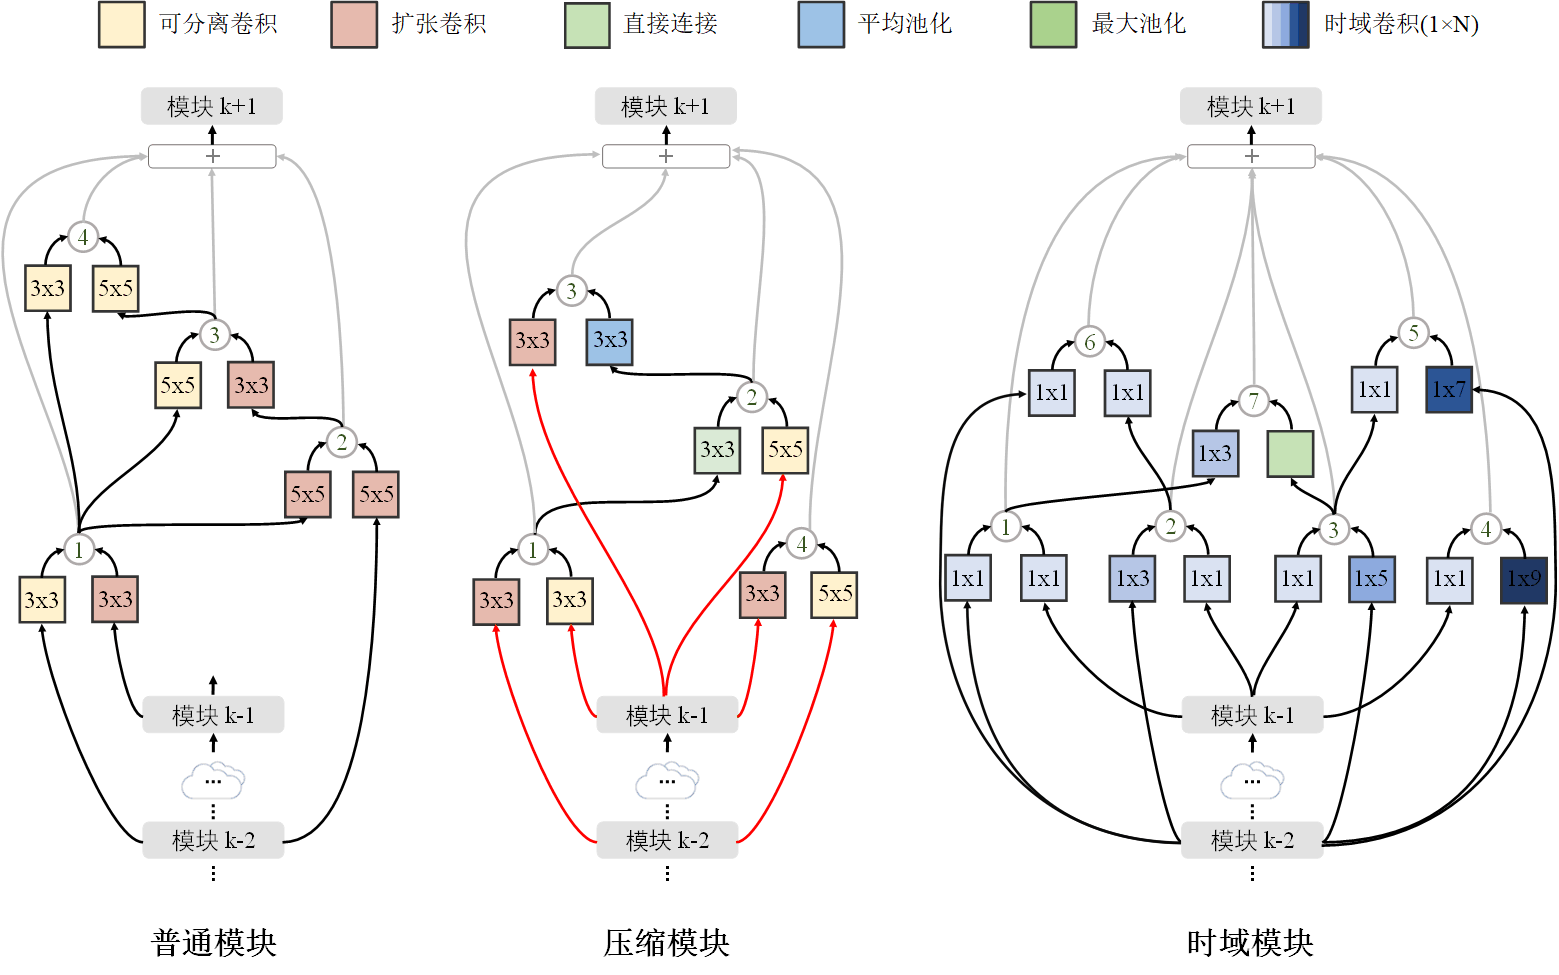
\includegraphics[width=0.61\textheight]{SEED模块.png}
	\caption{SEED数据集上搜索到的三种模块结构} 
	\label{fig3-4}
\end{figure}


\begin{table*}[!h]
\caption{SEED数据集上获得的CNN架构的详细参数}  \label{tab3-2}
\centering
\wuhao{
    \begin{threeparttable}
    \setlength{\tabcolsep}{3mm}{
        \begin{tabular}{cccc}
            \toprule
            \textbf{模块}   &  \textbf{节点} &  \textbf{输入}   &  \textbf{选取的操作}\\ 
            \midrule
            
            \multirow{4}*{普通模块} &节点1     &$concat$(模块k-2,模块k-1)   &3×3可分离卷积,3×3扩张卷积    \\
                                   &节点2     &$concat$(模块k-2,节点1)   &5×5扩张卷积,5×5扩张卷积    \\
                                   &节点3     &$concat$(节点1,节点2)   &5×5可分离卷积,3×3扩张卷积    \\
                                   &节点4     &$concat$(节点1,节点3)   &3×3可分离卷积,5×5可分离卷积    \\
            \midrule
            \multirow{4}*{压缩模块} &节点1     &$concat$(模块k-2,模块k-1)   &3×3扩张卷积,3×3可分离卷积    \\
                                   &节点2     &$concat$(模块k-1,节点1)   &5×5可分离卷积,3×3最大池化    \\
                                   &节点3     &$concat$(模块k-1,节点2)   &3×3扩张卷积,3×3平均池化    \\
                                   &节点4     &$concat$(模块k-2,模块k-1)   &5×5可分离卷积,3×3扩张卷积    \\
            \midrule
            \multirow{7}*{时域模块} &节点1     &$concat$(模块k-2,模块k-1)   &1×1时域卷积,1×1时域卷积    \\
                                   &节点2     &$concat$(模块k-2,模块k-1)   &1×3时域卷积,1×1时域卷积    \\
                                   &节点3     &$concat$(模块k-2,模块k-1)   &1×5时域卷积,1×1时域卷积    \\
                                   &节点4     &$concat$(模块k-2,模块k-1)   &1×9时域卷积,1×1时域卷积    \\
                                   &节点5     &$concat$(模块k-2,节点3)   &1×7时域卷积,1×1时域卷积    \\
                                   &节点6     &$concat$(模块k-2,节点2)   &1×1时域卷积,1×1时域卷积    \\
                                   &节点7     &$concat$(节点1,节点3)   &1×3时域卷积,直接连接    \\
            \bottomrule
        \end{tabular}
        }
        \begin{tablenotes}
	    \footnotesize
	    \item $concat$: 指串联操作(concatenate)。
    \end{tablenotes}
    \end{threeparttable}
    }
\end{table*}




(2) 分类结果

表\ref{tab3-3}给出了所提出的模型和对比算法在SEED数据集上的分类结果。所有的方法都使用了全部62个通道的数据,并使用LOSO交叉验证方案。作为一个典型的神经网络模型,本节所提出的方法会因为随机种子的变化而产生不同的初始化结果,影响模型的最终分类性能。经过多次试验,本模型在SEED数据集上的平均分类精度分布在0.81到0.84之间。在表\ref{tab3-3}中,给出了多次试验后的分类结果中间值。

\begin{table*}[!h]
\caption{SEED数据集不同频段的分类结果(平均值\%/标准差)以及模型复杂度}  \label{tab3-3}
\centering
\wuhao{
    \begin{threeparttable}
    \setlength{\tabcolsep}{0.20mm}{
        \begin{tabular}{cccccccc}
            \toprule
            \multirow{2}*{\textbf{模型}}   &  \multirow{2}*{\textbf{$\delta$}\textbf{频段}} &  \multirow{2}*{\textbf{$\theta$}\textbf{频段}}   & \multirow{2}*{ \textbf{$\alpha$}\textbf{频段}} & \multirow{2}*{\textbf{$\beta$}\textbf{频段}} &  \multirow{2}*{\textbf{$\gamma$}\textbf{频段}} &  \multirow{2}*{\textbf{全频段}} &  \textbf{模型复杂度}\\ 
            &&&&&& &\textbf{参数量(M)}\\
            \midrule          
            TCA\cite{3-19} &44.10/8.22     &41.26/9.21   &42.93/14.33 &43.93/10.06 &48.43/9.73 &63.64/14.88 &$\mathrm{O}\left(\mathrm{n}^2 \mathrm{~d}\right)$     \\
            DANN\cite{3-20} &-     &-   &- &- &- &75.08/11.18 &0.2573     \\
            Cimtay等人\cite{3-21} &-     &-   &- &- &- &78.34 &-     \\
            Fdez等人\cite{3-22} &-     &-   &- &- &- &79.60/10.40 &0.0250     \\
            DGCNN\cite{3-23} &49.79/10.94     &46.36/12.06   &48.29/12.28 &56.15/14.01 &54.87/17.53 &79.95/9.02 &-     \\
            ASFM\cite{3-24} &-     &-   &- &- &- &80.46/6.84 &-     \\
            LF+BiLSTM\cite{3-25} &-    &-   &- &- &- &81.04/6.88 &-     \\
            CNN-DDC\cite{3-26} &-     &-   &- &- &- &82.16/4.43 &-     \\
            BiDANN-S\cite{3-27} &63.01/7.49     &63.22/7.52   &63.50/9.50 &73.59/9.12 &73.72/8.67 &84.14/6.87 & -    \\
            RGNN\cite{3-28} &64.88/6.87     &60.69/5.79   &60.84/7.57 &74.96/8.94 &77.50/8.10 &85.30/6.72 &0.4468     \\
            本章模型 &59.70/13.50     &62.37/7.32   &67.85/8.27 &71.85/8.02 &73.04/ 6.33 &82.96/ 7.85 &0.3795     \\
            \midrule
            频域流     &59.81/ 13.61   &62.08/7.41 &67.96/8.55 &70.32/7.99 &72.65/6.28 &81.82/ 7.96 & 0.2054    \\
            时域流     &-    &-   &- &- &- &48.35/ 6.96 &0.0890     \\
        
            \bottomrule
        \end{tabular}
        }
        \begin{tablenotes}
	    \footnotesize
	    \item -: 模型不具有或未公开相应细节。
    \end{tablenotes}
    \end{threeparttable}
    }
\end{table*}

在单个频段的对比中,本节将输入特征从五个频段更换为单一频段,同时微调模型的输入节点以适应输入维度的变化。对于单个频段,本章所提出的模型在$\alpha$频段取得了所有方法中最高的分类精度;在$\theta$频段也取得了第二高的结果;并且在$\gamma$频段同样具有竞争力。在全部频段上,本章的模型取得了第三高的分类准确率,同时具有可接受的标准差。从准确率的角度来看,本方法在单一频段极具竞争力,在全频段接近于最先进的对比模型,并且优于大多数模型。虽然总体准确率低于RGNN和BiDANN-S,但本方法避免了模型设计过程,在不同的数据集上拥有更好的泛化性能。在SEED数据集上,本章模型的MF1分数为0.8247,AUC值为0.9224。高兴、悲伤和中性三个类别的F1分数分别为0.8287、0.8231和0.8164。从F1分数的角度看,搜索得到的CNN模型对三种不同的情绪类别具有相似的分类能力,对高兴情绪的识别精度最高。从参数规模来看,DANN、RGNN和本章模型具有相同的数量级,但本模型能够取得比DANN更好的判别精度。另一方面,虽然准确率低于RGNN,但本模型的参数数也少于RGNN。Fdez等人提出的模型\cite{3-22}参数数量比其他方法少得多,但需要进行复杂的特征预处理过程才能达到最佳性能。所有的结果都表明,本章所提出的模型对情感分类任务是有效的。

(3) 消融实验

在消融实验中,为了证明当前网络结构的合理性,分别在只有时域流或频域流的搜索空间中搜索网络结构,其分类准确率在表\ref{tab3-3}中给出。如表所示,无论去除哪一部分,模型的最终分类性能都会下降,尤其是去除频域流后。可以看出,时域流在引入了一定数量的参数的同时,对分类精度的提升并不显著,但这一结构的存在是必要的,原因如下。首先,近年来,大量的研究人员致力于探索针对SEED数据集的算法,这使得不同算法之间的竞争非常激烈。从表\ref{tab3-3}中可知,不同算法之间往往只有1\%的性能差异,因此时域流带来的模型性能改进是值得保留的。其次,从表\ref{tab3-4}可以看出,时域流引入的参数数量比频域流少得多,对前向传播时间的影响也极其有限。从本质上讲,时域流带来的参数增加主要来自于模型末端的两个全连接层的变化,而时域流本身并没有引入过多的参数。同时,模型的前向传播时间主要取决于输入数据的维度,而时域流带来的模型复杂度的增加对前向传播时间的影响很小。此外,时域流的影响主要作用在搜索成本增加,即搜索模型架构的时间增长。一旦网络架构被确定,这种影响就会变得非常小,即一旦搜索到网络的最佳架构,本章算法的复杂度不会对使用者产生实质性影响。因此,保留时域流是值得的。本章的方法在Pytorch环境中实现,使用AMD CPU(R9-3950X,3.50 GHz)和NVIDIA GPU(RTX 3090)。
\begin{table*}[!h]
\caption{不同结构模型的时间复杂度}  \label{tab3-4}
\centering
\wuhao{
    \begin{threeparttable}
    \setlength{\tabcolsep}{1.3mm}{
        \begin{tabular}{cccccccccc}
            \toprule
            \multirow{2}*{\textbf{架构类型}}   & \multicolumn{3}{c}{\textbf{SEED}}  & \multicolumn{3}{c}{\textbf{JS-MI}} & \multicolumn{3}{c}{\textbf{疲劳}}\\ 
            &  \textbf{双流} &  \textbf{时域流}   &  \textbf{频域流} &  \textbf{双流} &  \textbf{时域流}   &  \textbf{频域流} &  \textbf{双流} &  \textbf{时域流} &  \textbf{频域流}\\ 
            \midrule          
            搜索耗时 &\multirow{2}*{17.52}     &\multirow{2}*{4.24}   &\multirow{2}*{13.15} &\multirow{2}*{14.47} &\multirow{2}*{3.83} &\multirow{2}*{10.25} &\multirow{2}*{11.67} &\multirow{2}*{2.61} &\multirow{2}*{8.74}\\
            (GPU-hours)&&&&&&&&& \\
            前向传播时间 &\multirow{2}*{2.8765}     &\multirow{2}*{0.7017}   &\multirow{2}*{1.9375} &\multirow{2}*{3.7456} &\multirow{2}*{2.4526} &\multirow{2}*{1.0265} &\multirow{2}*{0.0190} &\multirow{2}*{0.0080} &\multirow{2}*{0.0070}\\
            (Second)&&&&&&&&& \\     
            \bottomrule
        \end{tabular}
        }
    \end{threeparttable}
    }
\end{table*}


\subsection{疲劳驾驶检测公开数据集分类结果}
(1) 结构搜索进程

在疲劳辨识数据集上,使用NAS算法成功获得了相应的CNN架构。与SEED数据集不同,基于疲劳驾驶检测数据集的CNN架构更加简化。从图\ref{fig3-5}中可以看出,在频域流中的模块堆叠数到达两个,时域流中的内部节点数到达四个之前,网络一直处于过拟合状态,算法始终倾向于在两个流中使用弱参数操作。图\ref{fig3-6}给出了NAS过程得到的最终疲劳辨识CNN架构,具体的网络架构在表\ref{tab3-5}中给出。由于最终得到的频域流中模块堆叠数为2,根据堆叠原则,频域流仅包含普通模块,没有压缩模块。

\begin{table*}[!h]
\caption{疲劳驾驶检测数据集上获得的CNN架构的详细参数}  \label{tab3-5}
\centering
\wuhao{
    \begin{threeparttable}
    \setlength{\tabcolsep}{3mm}{
        \begin{tabular}{cccc}
            \toprule
            \textbf{模块}   &  \textbf{节点} &  \textbf{输入}   &  \textbf{选取的操作}\\ 
            \midrule
            
            \multirow{4}*{普通模块} &节点1     &$concat$(模块k-2,模块k-1)   &5×5可分离卷积,直接连接   \\
                                   &节点2     &$concat$(模块k-2,节点1)   &5×5可分离卷积,3×3扩张卷积    \\
                                   &节点3     &$concat$(模块k-2,节点1)   &5×5可分离卷积,直接连接    \\
                                   &节点4     &$concat$(模块k-2,节点2)   &5×5可分离卷积,3×3可分离卷积    \\
    
            \midrule
            \multirow{4}*{时域模块} &节点1     &$concat$(模块k-2,模块k-1)   &1×5时域卷积,1×5时域卷积    \\
                                   &节点2     &$concat$(模块k-2,模块k-1)   &1×5时域卷积,1×7时域卷积    \\
                                   &节点3     &$concat$(模块k-2,模块k-1)   &1×5时域卷积,1×5时域卷积    \\
                                   &节点4     &$concat$(模块k-1,节点1)   &1×1时域卷积,直接连接    \\
            \bottomrule
        \end{tabular}
        }
        \begin{tablenotes}
	    \footnotesize
	    \item $concat$: 指串联操作(concatenate)。
    \end{tablenotes}
    \end{threeparttable}
    }
\end{table*}

同样,为了证明早停算法的有效性,分别比较了重新训练前不同深度模型的验证集分类结果,结果如图\ref{fig3-5}(b)所示。在图中,验证集的准确率不断增加,在当前的网络结构下达到一个峰值。此外,当网络从当前的最佳结构进一步开始简化后,训练集的准确率开始下降,模型表征能力开始不足。

\begin{figure}[!h]
	\centering
	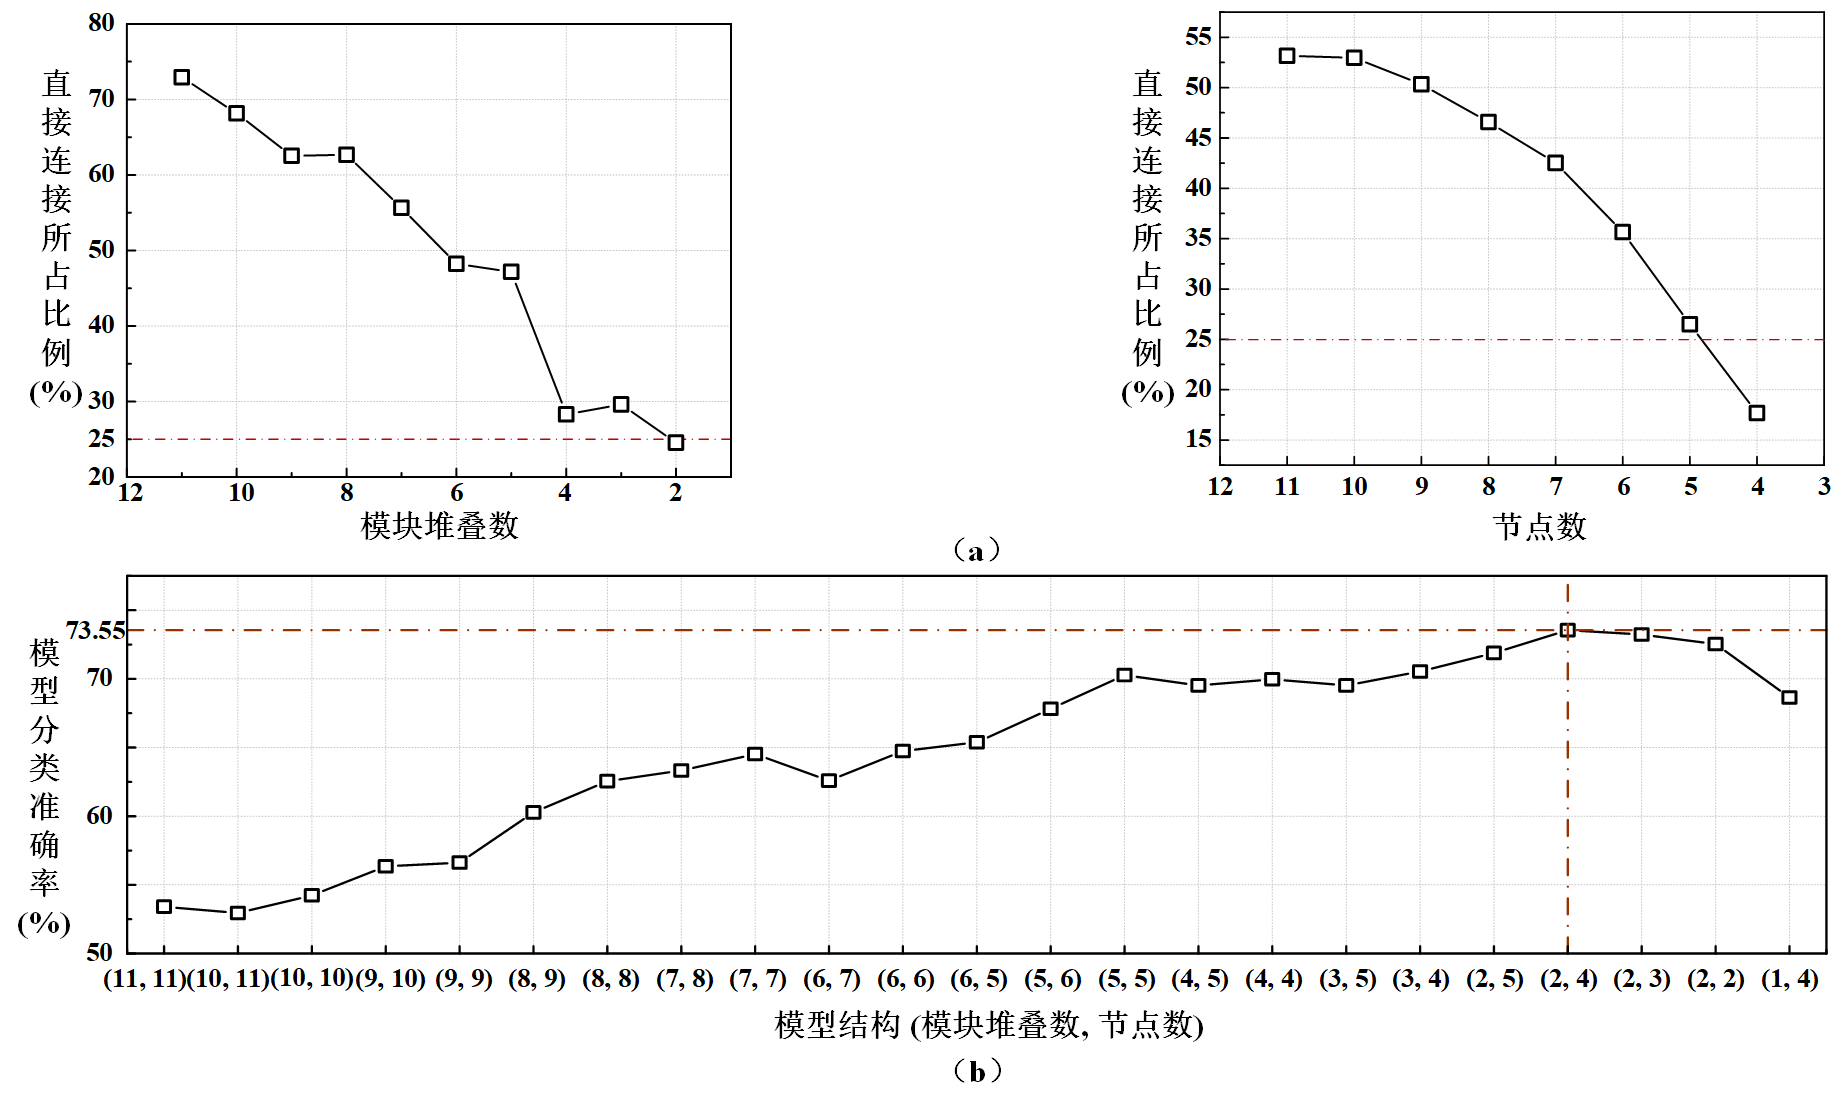
\includegraphics[width=0.60\textheight]{疲劳消融.png}
	\caption{疲劳驾驶检测数据集网络搜索进程} 
	\label{fig3-5}
\end{figure}

\begin{figure}[!h]
	\centering
	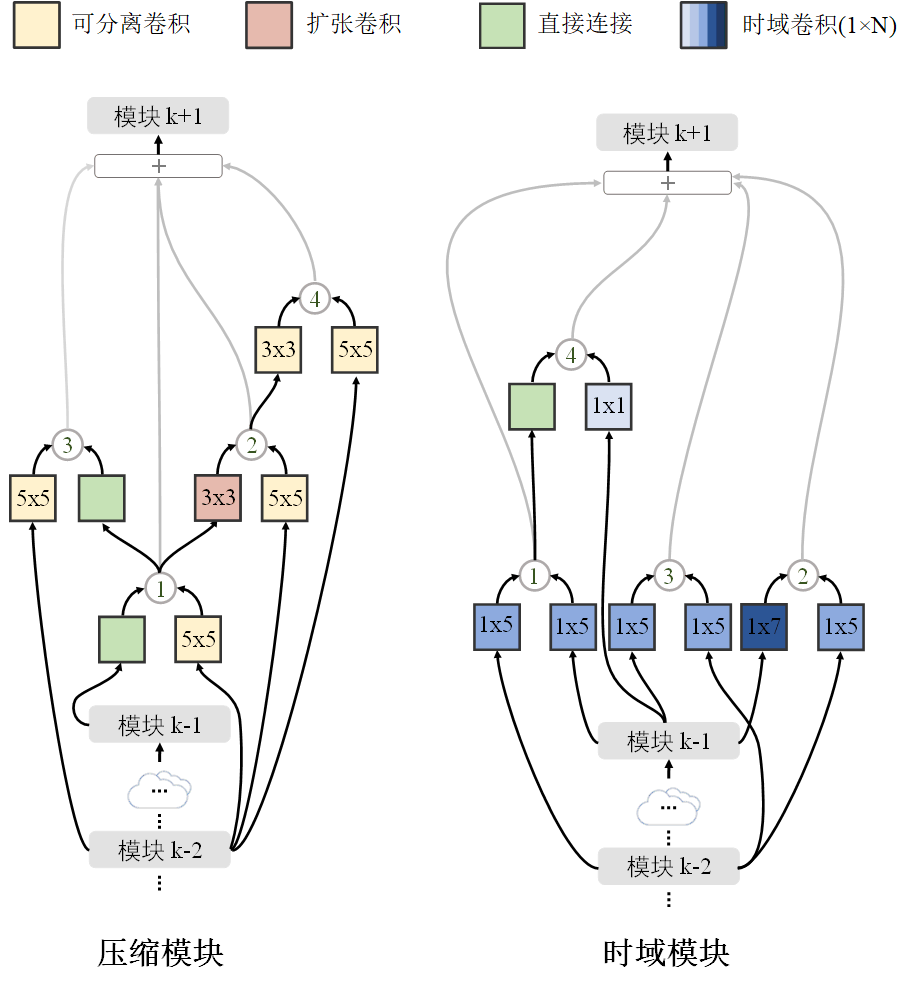
\includegraphics[width=0.40\textheight]{疲劳模块.png}
	\caption{疲劳驾驶检测数据集上搜索到的两种模块结构} 
	\label{fig3-6}
\end{figure}


(2) 分类结果 

由表\ref{tab3-6}可以看到,通过搜索得到的结构能够达到很好的分类效果,其在21个被试上的平均准确率为84.63\%,标准差为7.79。每个被试的准确率如图\ref{fig3-7}所示。表\ref{tab3-6}给出了所提出的模型架构和其他一些基于相同数据集的算法的分类结果,包括每种算法的分类准确率和被试间的标准差。由于标签获取方法的不同,每个算法所使用的数据集会略有不同。为了保证比较的公平性,所有的方法都将基于本文中的数据集进行复现,并使用LOSO交叉验证方案。如前文所述,为了减少随机种子带来的影响,表\ref{tab3-6}的结果是多次运行结果的中间值。值得注意的是,与同样基于EEG图像的算法\cite{3-32}相比,基于NAS算法得到的CNN架构能够达到比人工设计的CNN架构更好的识别精度,这证明了NAS根据当前数据和特征自动设计最佳网络架构时的高度优越性。表\ref{tab3-6}中显示的AUC值和MF1得分显示,本章的NAS策略对疲劳状态识别也很有效。从参数数量的角度来看,虽然本章的方法具有较高的模型复杂度,但它的识别精度也远远高于其他方法,所以认为本章的模型具有足够的竞争力。

\begin{table*}[!t]
\caption{疲劳驾驶检测数据集的分类结果(平均值\%/标准差)以及模型复杂度}  \label{tab3-6}
\centering
\wuhao{
    \begin{threeparttable}
    \setlength{\tabcolsep}{4.8mm}{
        \begin{tabular}{ccccc}
            \toprule
            \multirow{2}*{\textbf{模型}}   &  \multirow{2}*{\textbf{MF1}} &  \multirow{2}*{\textbf{AUC}}   &  \multirow{2}*{\textbf{全频段}} &  \textbf{模型复杂度}\\ 
            &&&&\textbf{参数量(M)}\\
            \midrule          
            EEGNet-4,2\cite{4-2} &59.01     &70.37   &61.87/8.41 &0.0049\\
            LR\cite{3-29} &62.53    &69.98  &61.92/8.54 &$\mathrm{O}\left(\mathrm{n} \mathrm{~d}\right)$     \\
            EEGNet-8,2\cite{4-2} &65.47     &74.67   &66.72/12.03 &0.0073\\
            CNN\cite{3-30} &70.11     &79.36   &70.28/9.66 &0.0143 \\
            TCA+LR\cite{3-19} &71.67     &80.71   &73.41/9.77 &$\mathrm{O}\left(\mathrm{n}^2 \mathrm{~d}+\mathrm{nd}\right)$ \\
            HCNN\cite{3-31} &74.35     &85.73   &75.65/9.84 &0.0035 \\
            Single Frame EEG Image\cite{3-32} &76.85    &89.65   &77.52/11.17 &0.0360   \\
            Temporal EEG Image\cite{3-32} &79.96     &90.36   &80.29/10.95 &0.0363 \\
            本章模型 &84.57     &93.47   &84.63/7.79 &0.2032\\
            \midrule
            频域流     &82.93   &91.82 &83.33/ 7.68 &0.0566 \\
            时域流     &68.56    &83.76   &69.91/ 7.23 &0.0611 \\
        
            \bottomrule
        \end{tabular}
        }
    \end{threeparttable}
    }
\end{table*}

(3) 消融实验

消融实验的实现过程与SEED数据集相同。从表\ref{tab3-6}可以看出,单流结构不足以达到与目前双流结构相同的分类精度,这证明了模型设计的合理性。同样,基于EEG图像的频域流获得了与双流网络类似的分类结果。频域流和时域流各自的计算资源消耗比较见表\ref{tab3-4}。在疲劳数据集上,由于输入数据量较小,而且特征的复杂度较低,所以搜索得到的模型参数数量比在SEED数据集上小得多。尽管由于引入了时域流,模型参数的规模增大了两倍,但考虑到模型本身较低的参数量级,依然认为参数数量的增加对模型的性能没有产生根本的影响。引入时域流后,模型搜索时间增加了2倍多,但前向传播时间仍在毫秒量级内,这对现实应用不会产生过量影响。然而,当追求效率和更少的资源消耗时,单独搜索频域流毫无疑问是一个更具竞争力的选择。

\begin{figure}[!h]
	\centering
	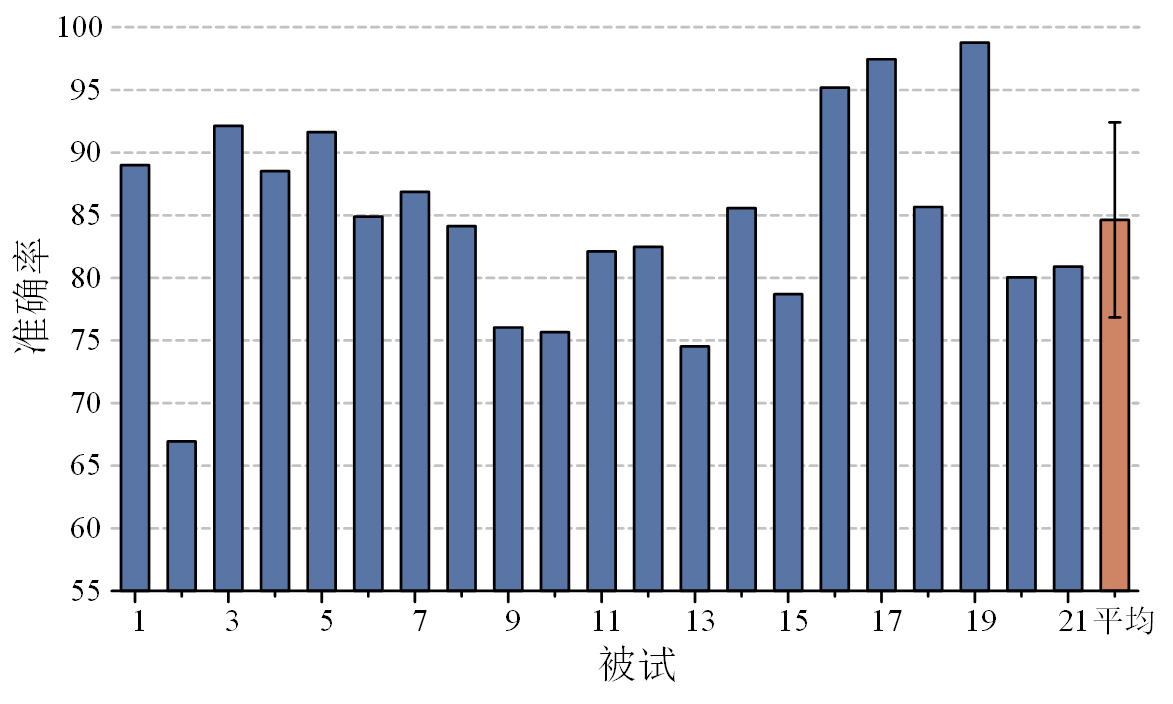
\includegraphics[width=0.45\textheight]{疲劳所有被试.png}
	\caption{疲劳驾驶检测数据集所有被试分类结果} 
	\label{fig3-7}
\end{figure}


\subsection{JS-AINS-40采集的情绪辨识数据集分类结果}

(1) 结构搜索进程

由图\ref{fig3-8}(a)可知,在JS-EM数据集上,直接连接在所有操作中所占的比例依然是判别模型当前拟合状态的有效指标。在直接连接比例低于25\%时,模型获得了在验证集上最优的辨识结果。

\begin{figure}[!h]
	\centering
	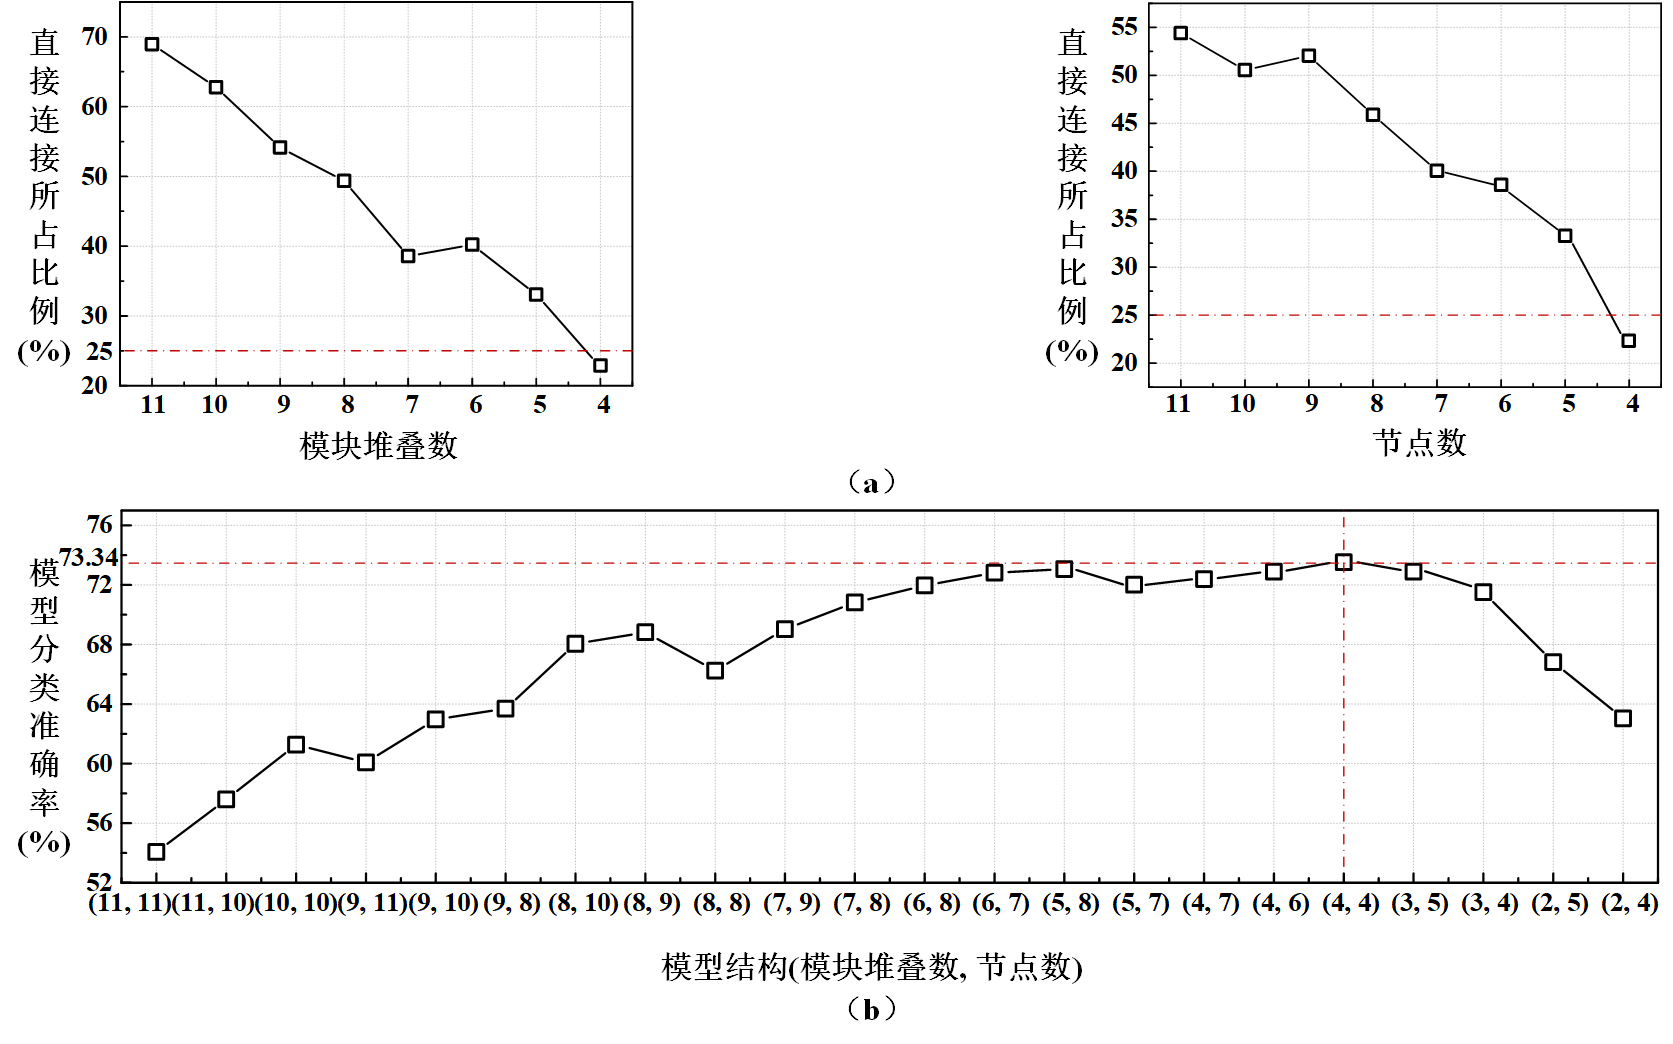
\includegraphics[width=0.60\textheight]{JS-EM消融.png}
	\caption{JS-EM数据集网络搜索进程} 
	\label{fig3-8}
\end{figure}

由于JS-EM数据集所包含的样本量和电极通道数少于SEED数据集,因此模型搜索到的结构也更加简单。由图\ref{fig3-8}(b)可知,在JS-EM数据集上,当频域流堆叠的模块数为4,时域流内部的节点数也为4时,模型在验证集上表现最佳。这证明了搜索得到的模型结构的合理性。各个模块具体的内部结构如图\ref{fig3-9}和表\ref{tab3-8}。由于频域流模块堆叠数量为4,因此其包含普通模块和压缩模块两种单元。

可以看出,早停算法和自适应算法的引入,成功让NAS算法适应了JS-EM数据集。这不仅验证了算法的有效性,也证明了JS-AINS-40系统所采集数据的可靠性。

\begin{figure}[!h]
	\centering
	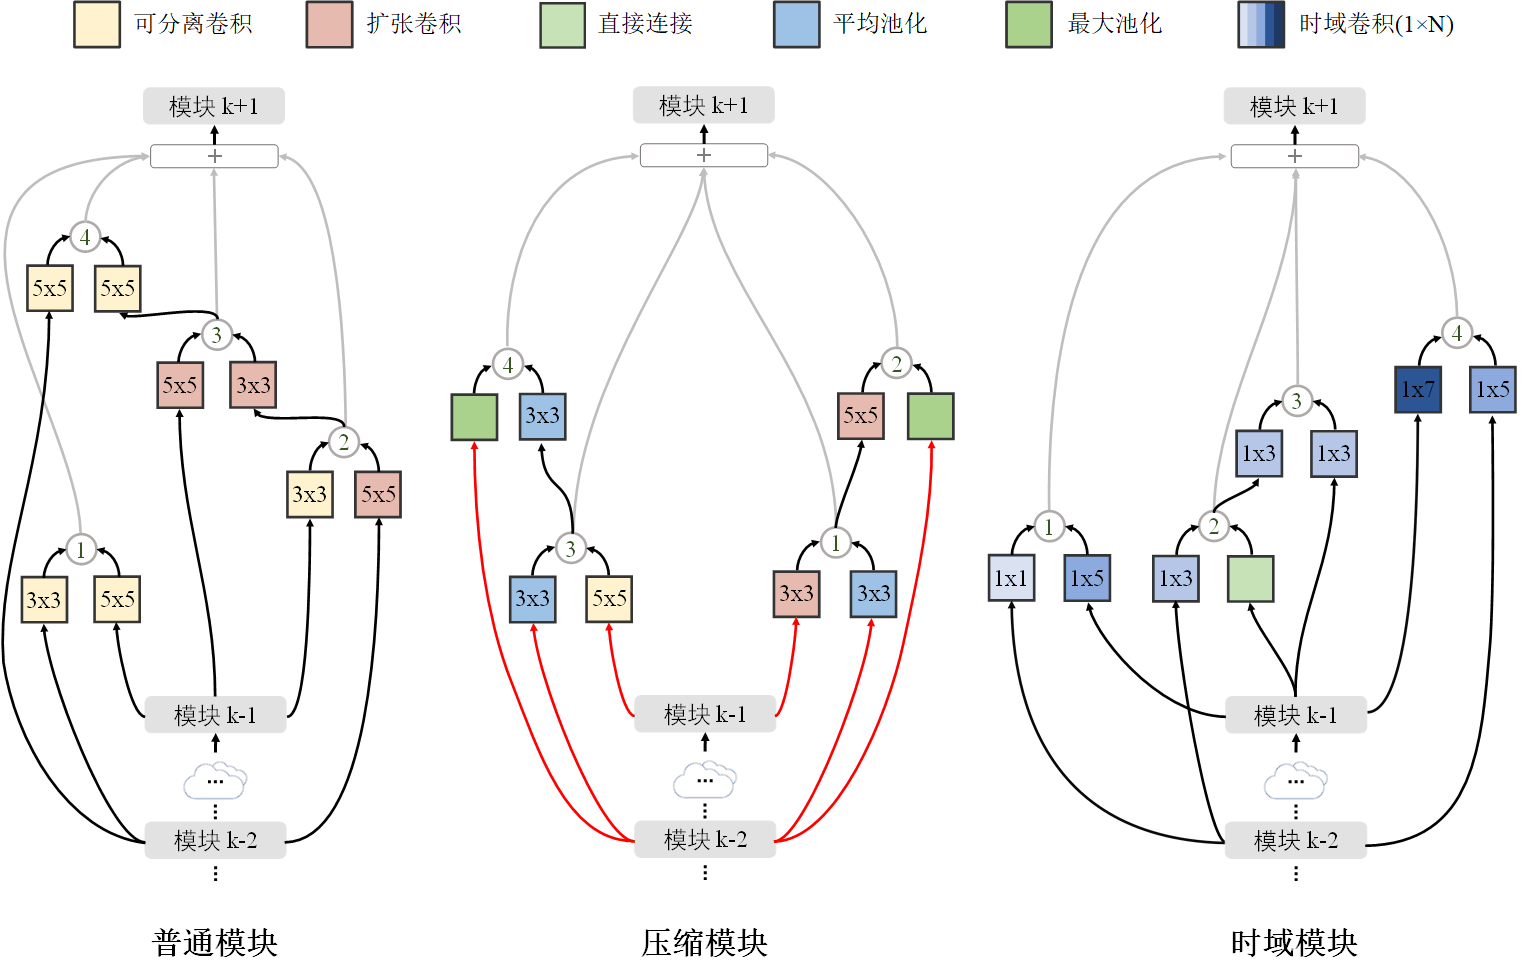
\includegraphics[width=0.60\textheight]{JS-EM模块.png}
	\caption{JS-EM数据集上搜索到的三种模块结构} 
	\label{fig3-9}
\end{figure}

\begin{table*}[!h]
\caption{JS-EM数据集上获得的CNN架构的详细参数}  \label{tab3-8}
\centering
\wuhao{
    \begin{threeparttable}
    \setlength{\tabcolsep}{3mm}{
        \begin{tabular}{cccc}
            \toprule
            \textbf{模块}   &  \textbf{节点} &  \textbf{输入}   &  \textbf{选取的操作}\\ 
            \midrule
            
            \multirow{4}*{普通模块} &节点1     &$concat$(模块k-2,模块k-1)   &3×3可分离卷积,5×5可分离卷积    \\
                                   &节点2     &$concat$(模块k-2,模块k-1)   &5×5扩张卷积,3×3可分离卷积    \\
                                   &节点3     &$concat$(模块k-1,节点2)     &5×5扩张卷积,3×3扩张卷积    \\
                                   &节点4     &$concat$(模块k-2,节点3)     &5×5可分离卷积,5×5可分离卷积    \\
            \midrule
            \multirow{4}*{压缩模块} &节点1     &$concat$(模块k-2,模块k-1)   &3×3平均池化,3×3扩张卷积    \\
                                   &节点2     &$concat$(模块k-2,节点1)     &直接连接,5×5扩张卷积    \\
                                   &节点3     &$concat$(模块k-2,模块k-1)   &3×3平均池化,5×5可分离卷积    \\
                                   &节点4     &$concat$(模块k-2,节点3)     &直接连接,3×3平均池化    \\
            \midrule
            \multirow{4}*{时域模块} &节点1     &$concat$(模块k-2,模块k-1)   &1×1时域卷积,1×5时域卷积    \\
                                   &节点2     &$concat$(模块k-2,模块k-1)   &1×3时域卷积,直接连接    \\
                                   &节点3     &$concat$(模块k-1,节点2)   &1×3时域卷积,1×3时域卷积    \\
                                   &节点4     &$concat$(模块k-2,模块k-1)   &1×5时域卷积,1×7时域卷积    \\
            \bottomrule
        \end{tabular}
        }
        \begin{tablenotes}
	    \footnotesize
	    \item $concat$: 指串联操作(concatenate)。
    \end{tablenotes}
    \end{threeparttable}
    }
\end{table*}


\begin{table*}[!h]
\caption{JS-EM数据集不同频段的分类结果(平均值\%/标准差)以及模型复杂度}  \label{tab3-9}
\centering
\wuhao{
    \begin{threeparttable}
    \setlength{\tabcolsep}{0.15mm}{
        \begin{tabular}{cccccccc}
            \toprule
            \multirow{2}*{\textbf{模型}}   &  \multirow{2}*{\textbf{$\delta$}\textbf{频段}} &  \multirow{2}*{\textbf{$\theta$}\textbf{频段}}   & \multirow{2}*{ \textbf{$\alpha$}\textbf{频段}} & \multirow{2}*{\textbf{$\beta$}\textbf{频段}} &  \multirow{2}*{\textbf{$\gamma$}\textbf{频段}} &  \multirow{2}*{\textbf{全频段}} &  \textbf{模型复杂度}\\
            &&&&&&&\textbf{参数量(M)}\\
            \midrule          
            TCA\cite{3-19} &41.46/8.35     &40.07/9.32   &39.50/11.26 &42.48/11.14 &46.41/8.72 &60.35/13.97 
            
            &$\mathrm{O}\left(\mathrm{n}^2 \mathrm{~d}\right)$     \\
  
  
            DANN\cite{3-20} &-     &-   &- &- &- &71.90/12.41 &0.2216     \\

            
            Fdez等人\cite{3-22}     &-     &-   &- &- &- &75.01/9.94 &0.0194     \\
            
            
            RGNN\cite{3-28}   &62.45/6.54     &60.23/6.08   &60.79/7.68 &71.98/8.11 &72.63/7.95 &80.92/6.67 &0.3951     \\
          
            本章模型           &58.15/13.77     &59.76/7.04   &63.59/8.56 &68.09/7.63 &69.58/6.20 &78.50/7.51 &0.3043     \\
            \midrule
            频域流     &58.04/ 14.32   &59.06/7.89 &63.42/8.43 &68.04/7.85 &68.11/6.37 &77.84/8.18 & 0.1783    \\
            时域流     &-    &-   &- &- &- &42.98/ 7.08 &0.0687     \\
        
            \bottomrule
        \end{tabular}
        }
        \begin{tablenotes}
	    \footnotesize
	    \item -: 模型不具有相应细节。
    \end{tablenotes}
    \end{threeparttable}
    }
\end{table*}

(2) 分类结果 

本章所提出算法的最终分类结果如表\ref{tab3-9}所示。本节选取了表\ref{tab3-3}中开源的对比方法对JS-EM数据集进行了评估,同时对比所提出算法的性能。由于本节的主要目的不在于验证算法的有效性,而是检验不同算法能否正确辨识JS-EM数据集,即JS-AINS-40系统采集的情绪EEG数据是否能够用来辨识人脑情绪状态。因此,这里仅引入了四种不同的对比方法。从结果可知,基于传统机器学习的情绪辨识算法、基于对抗学习的辨识方法以及基于图卷积的分类模型均在JS-EM数据集上获得了成功。这证明了JS-EM数据集的可靠性,并进一步验证了JS-AINS-40系统的稳定性。

在JS-EM数据集上,本章所提出模型的MF1分数为0.7992,AUC值为0.8807。高兴,悲伤,中性三个类别对应的F1分数分别为0.8011,0.7906,0.7858。模型依然对三种类别具有相近的分类能力,并且对高兴的辨识精度最高。

尽管在所有方法中,RGNN依然取得了最佳的分类结果,但是本章算法也仍然具有足够的竞争力,并且本章算法具有更低的模型空间复杂度。同样的,无需人工进行模型结构设计,依然是本章算法的最大优势。与表\ref{tab3-3}对比可知,所有方法在JS-EM数据集上的结果均低于SEED数据集。这主要源自于JS-EM数据集较少的通道数量和样本量,让算法更难以提取到足够具有辨识性的特征。但毫无疑问,JS-EM数据集上的结果依然处于可接受范围,这证明了JS-ANIS-40系统具备足够的可靠性。

(3) 消融实验

本节进行的消融实验,其具体内容与之前的数据集相同。在表\ref{tab3-9}中给出了单流结构的分类准确率,相应的时间消耗可以见表\ref{tab3-4}。可以看到,频域流在模型中依然占据主要作用。但是,在JS-EM数据集上,时域流的作用有所降低,添加时域流后,模型的准确率仅上升了不到0.7\%。这可能是由于本章使用了JS-EM数据集中全部40通道的EEG数据,模型没有直接获取关键特征,导致时域特征提供的帮助更为有限。然而,时域流的引入毫无疑问让模型的辨识能力获得了提升,并进一步降低了不同被试间结果的标准差,这证明了时域流的存在具有必要性。

虽然JS-EM数据集采用了与SEED相似的实验流程设计,但是由于被试人数,试验次数,EEG通道数等众多因素的影响,二者的最优模型结构仍具有较大的差异。这也进一步导致了基于二者的模型在空间复杂度(参数量)与时间复杂度(前向传播时间)上的差异。从结果可以看出,所提出算法在JS-EM数据集上同样具备足够的泛化性能。


\subsection{与其他NAS算法的比较}

在表\ref{tab3-7}中,除了RL-NAS\cite{3-33}之外,所有的模型都不能在未进行调整时在EEG数据上获得足够的分类精度(堆叠模块数量均被设定为8时)。这从另一个角度验证了本章对PC-DARTS改进的合理性。由于Robustified DARTS\cite{3-36}引入了更强的L2正则化和早停策略,这使得它在模型复杂度较高时取得了比PC-DARTS更好的结果。另一方面,RL-NAS不需要进行结构调整,因为这一模型结构是面向EEG信号而设计的。

\begin{table*}[!h]
\caption{不同NAS算法在疲劳驾驶检测数据集上的LOSO分类结果(平均值\%/标准差)}  \label{tab3-7}
\centering
\wuhao{
    \begin{threeparttable}
    \setlength{\tabcolsep}{4.1mm}{
        \begin{tabular}{ccc}
            \toprule
            \textbf{模型}   &  \textbf{未进行调整时的分类准确率} & \textbf{进行调整后的分类准确率} \\ 
            \midrule          
            RL-NAS\cite{3-33} &71.59/7.37     &71.59/7.37 \\
            DARTS\cite{3-34} &58.14/6.76     &76.54/8.02 \\
            SNAS\cite{3-35} &57.59/6.53    &77.41/7.90  \\
            Robustified DARTS\cite{3-36} &64.20/6.44     &82.57/7.53 \\
            本章模型 &62.58/6.37     &83.33/7.68   \\
        
            \bottomrule
        \end{tabular}
        }
    \end{threeparttable}
    }
\end{table*}

除了RL-NAS之外,所有NAS搜索算法的基础模型架构都过于复杂,在疲劳的数据集上会造成严重的过拟合问题,最终导致分类结果不佳。在此基础上进行比较是没有意义的。由于参与比较的模型都使用了与DARTS类似的架构,本节借用了本章中搜索得到的最佳网络结构——将对比模型中的堆叠模块数设置为2(除了RL-NAS),并在此基础上进行网络结构搜索。同时,使用EEG时间序列作为RL-NAS模型的输入,其余的对比模型都用EEG图像作为输入。

从表\ref{tab3-7}的最终结果可以看出,RL-NAS取得的分类精度与时域流接近,这是由于时域流的设计思路与RL-NAS相似,两者的模型结构也非常接近。然而,由于RL-NAS中的粒子群优化算法可以微调卷积操作的卷积核个数,使网络的性能得到了更多的提升——因此时域流的精度相对较低。但是,如果参考RL-NAS在本文的搜索空间中加入具有不同卷积核数量的卷积操作,将会导致搜索空间维度激增,带来搜索时间的大幅增加。考虑到这一改动将会带来的计算资源消耗,本章没有采用这一策略。

DARTS和SNAS都发表于2019年,依靠不同的算法进行网络架构搜索,但性能相似,因此取得了类似的分类结果。然而,由于两者都没有约束网络中弱参数操作的选取,因此在EEG上的性能并不理想。Robustified DARTS从不同的角度对NAS的崩塌进行了优化,增加了早停机制和针对“内部目标”的L2正则化系数,从而使分类结果优于DARTS和SNAS。然而,由于本章模型在PC-DARTS的边缘正则化算法基础上引入了针对性的改动,从而使其能够更好地应对NAS的崩塌现象,并在当前的数据集上取得较好的分类精度。同时,PC-DARTS的部分通道采样功能有效地减少了NAS过程中使用的显存大小,为本章的后续改进提供了关键性保障。

综上所述,对于当前的EEG辨识任务来说,本章提出的模型是足够先进的、具有竞争力的。

\section{本章小结}

本章在现有NAS技术基础上改进得到了一个新的模型,以获得基于EEG识别人脑生理状态的CNN框架。这是NAS技术在EEG信号辨识领域的一个创新应用。为了实现将基于图像的NAS技术向EEG时序信号的迁移,本章创新性地设计了一个基于先验知识的有限但合理的搜索空间。同时,为了找到合适的网络深度,降低崩塌的风险,本章引入了层数自适应机制和早停机制。在本章中,时域流被用来提取通道的时间依赖性和通道的具体特征,而频域流则更关注通道的相对位置及其频域特征。该模型的有效性在三个不同的EEG状态评估任务中被分别验证。结果表明,由NAS算法得到的CNN框架能够在情绪识别任务中取得具有竞争力的分类精度,并能在疲劳状态辨识任务中取得一定的优势。

上述结果说明,本章所提出的基于梯度自动优化的脑电辨识模型可以根据不同的数据集构建有针对性的网络架构,并具一定的有效性和通用性。因此,本章所提出的方法是NAS技术向EEG分析领域的有效迁移,并有很大潜力为其他类型的分类和预测任务提供高性能的结果。这可以有效降低研究人员的时间成本,促进CNN在更多领域的应用。

同时,在JS-EM数据集上的结果也证明了JS-AINS-40系统具备足够的可靠性。尽管JS-EM数据集在不同情绪分类算法中取得的结果略低于SEED数据集,但是这一差距依然在实验环境以及被试间差异可能导致的偏差区间内。因此,认为JS-AINS-40系统具备辨识人脑情绪状态的能力。







\clearpage{\pagestyle{empty}\cleardoublepage}
% !Mode:: "TeX:UTF-8"

\chapter{基于多被试动态迁移与迭代自训练的脑电辨识算法}
作为BCI中的一个重要分支,能够反应人脑运动意图的MI范式在运动障碍患者的康复过程中具有积极的作用。为了推广MI-BCI系统在现实场景下的应用,需要一种能够有效应对被试和时段间差异的强鲁棒性解码模型。大多数MI解码模型在应用前需要用有标注数据进行校准和训练,其性能依赖于特定被试和时段的特征。而在跨被试与跨时段场景下,这些解码模型的性能将出现大幅下降。其原因在于传统的深度学习模型往往假设训练集数据与测试集数据遵循相同的统计学分布,其特征位于相近的潜在空间中。在这一背景下,解码模型往往要求训练集数据与测试集数据采集自同一被试的同一时段,以达到期望的辨识性能。然而在实际场景中,因为受试者很难专注的进行长时间的EEG采集,这种需求将难以接受。毋庸置疑,在基于MI的残疾康复进程中,这一问题变得尤为明显。如何使用不同被试采集自不同时段的MI数据获得一个鲁棒的解码模型,是当前亟需解决的难题。

针对上述难题,本章将基于动态迁移与迭代自训练的域适应算法引入MI范式的BCI系统应用中。其包含一种能够促进域对齐的动态注意力模型以及囊括两个不同伪标签算法的迭代自训练策略。同时,本章引入了四组不同的运动想象数据集与八种不同的对比方法以评估所提出模型的有效性。四组数据集中包含三组公开数据集和一组使用JS-AINS-40设备采集的实验数据集。在四组数据集上的结果验证了本章所提出方法的泛化性能,同时证明了JS-AINS-40设备的可靠性。更进一步的,本章所提出的方法在四组数据集上均取得了超越所有对比方法的辨识性能,这进一步验证了该方法的优越性。


\section{基于多被试动态迁移与迭代自训练的脑电辨识算法}

本章提出了一种全新的无监督域适应方法——迭代自训练多被试域适应(Iterative Self-training Multi-subject Domain Adaptation,ISMDA),以解决离线MI-BCI系统在实际应用中遇到的问题,其体系结构如图\ref{fig_4_1}所示。该方法首先采用多通道时空滤波(Multi-channel Temporal-Spatial Filtering,MTSF)特征提取器将EEG信号映射到潜在空间。将特征提取过程匹配到不同MI动作所对应的大脑皮层活跃区域,让特征具有更强的临床解释性。为了减少对域信息的依赖,采用动态注意力模块(Dynamic Attention Module,DAM)消除源域之间的差异。同时,动态注意力模块在非对抗条件下完成了域对齐,使模型能够克服跨被试同时跨时段的难题。针对自训练机制中伪标签的源域偏向性问题,过度自信问题以及噪声问题,设计基于面向域分类器的迭代自训练(Domain-oriented Classifier-based Iterative Self-training,DCIS)。基于面向域分类器的迭代自训练包含两个不同的伪标签算法,分别为基于面向目标域的辅助分类器(Auxiliary Target Domain-Oriented Classifier,ATDOC)的伪标签算法以及基于确定性和置信度的伪标签算法(Pseudo-label Algorithm based on Certainty and Confidence,PACC)。两种算法对模型进行迭代自训练,显著提高了伪标签的可靠性,并将自训练方法与MI辨识任务有效结合。

\begin{figure*}[!t]
\centering
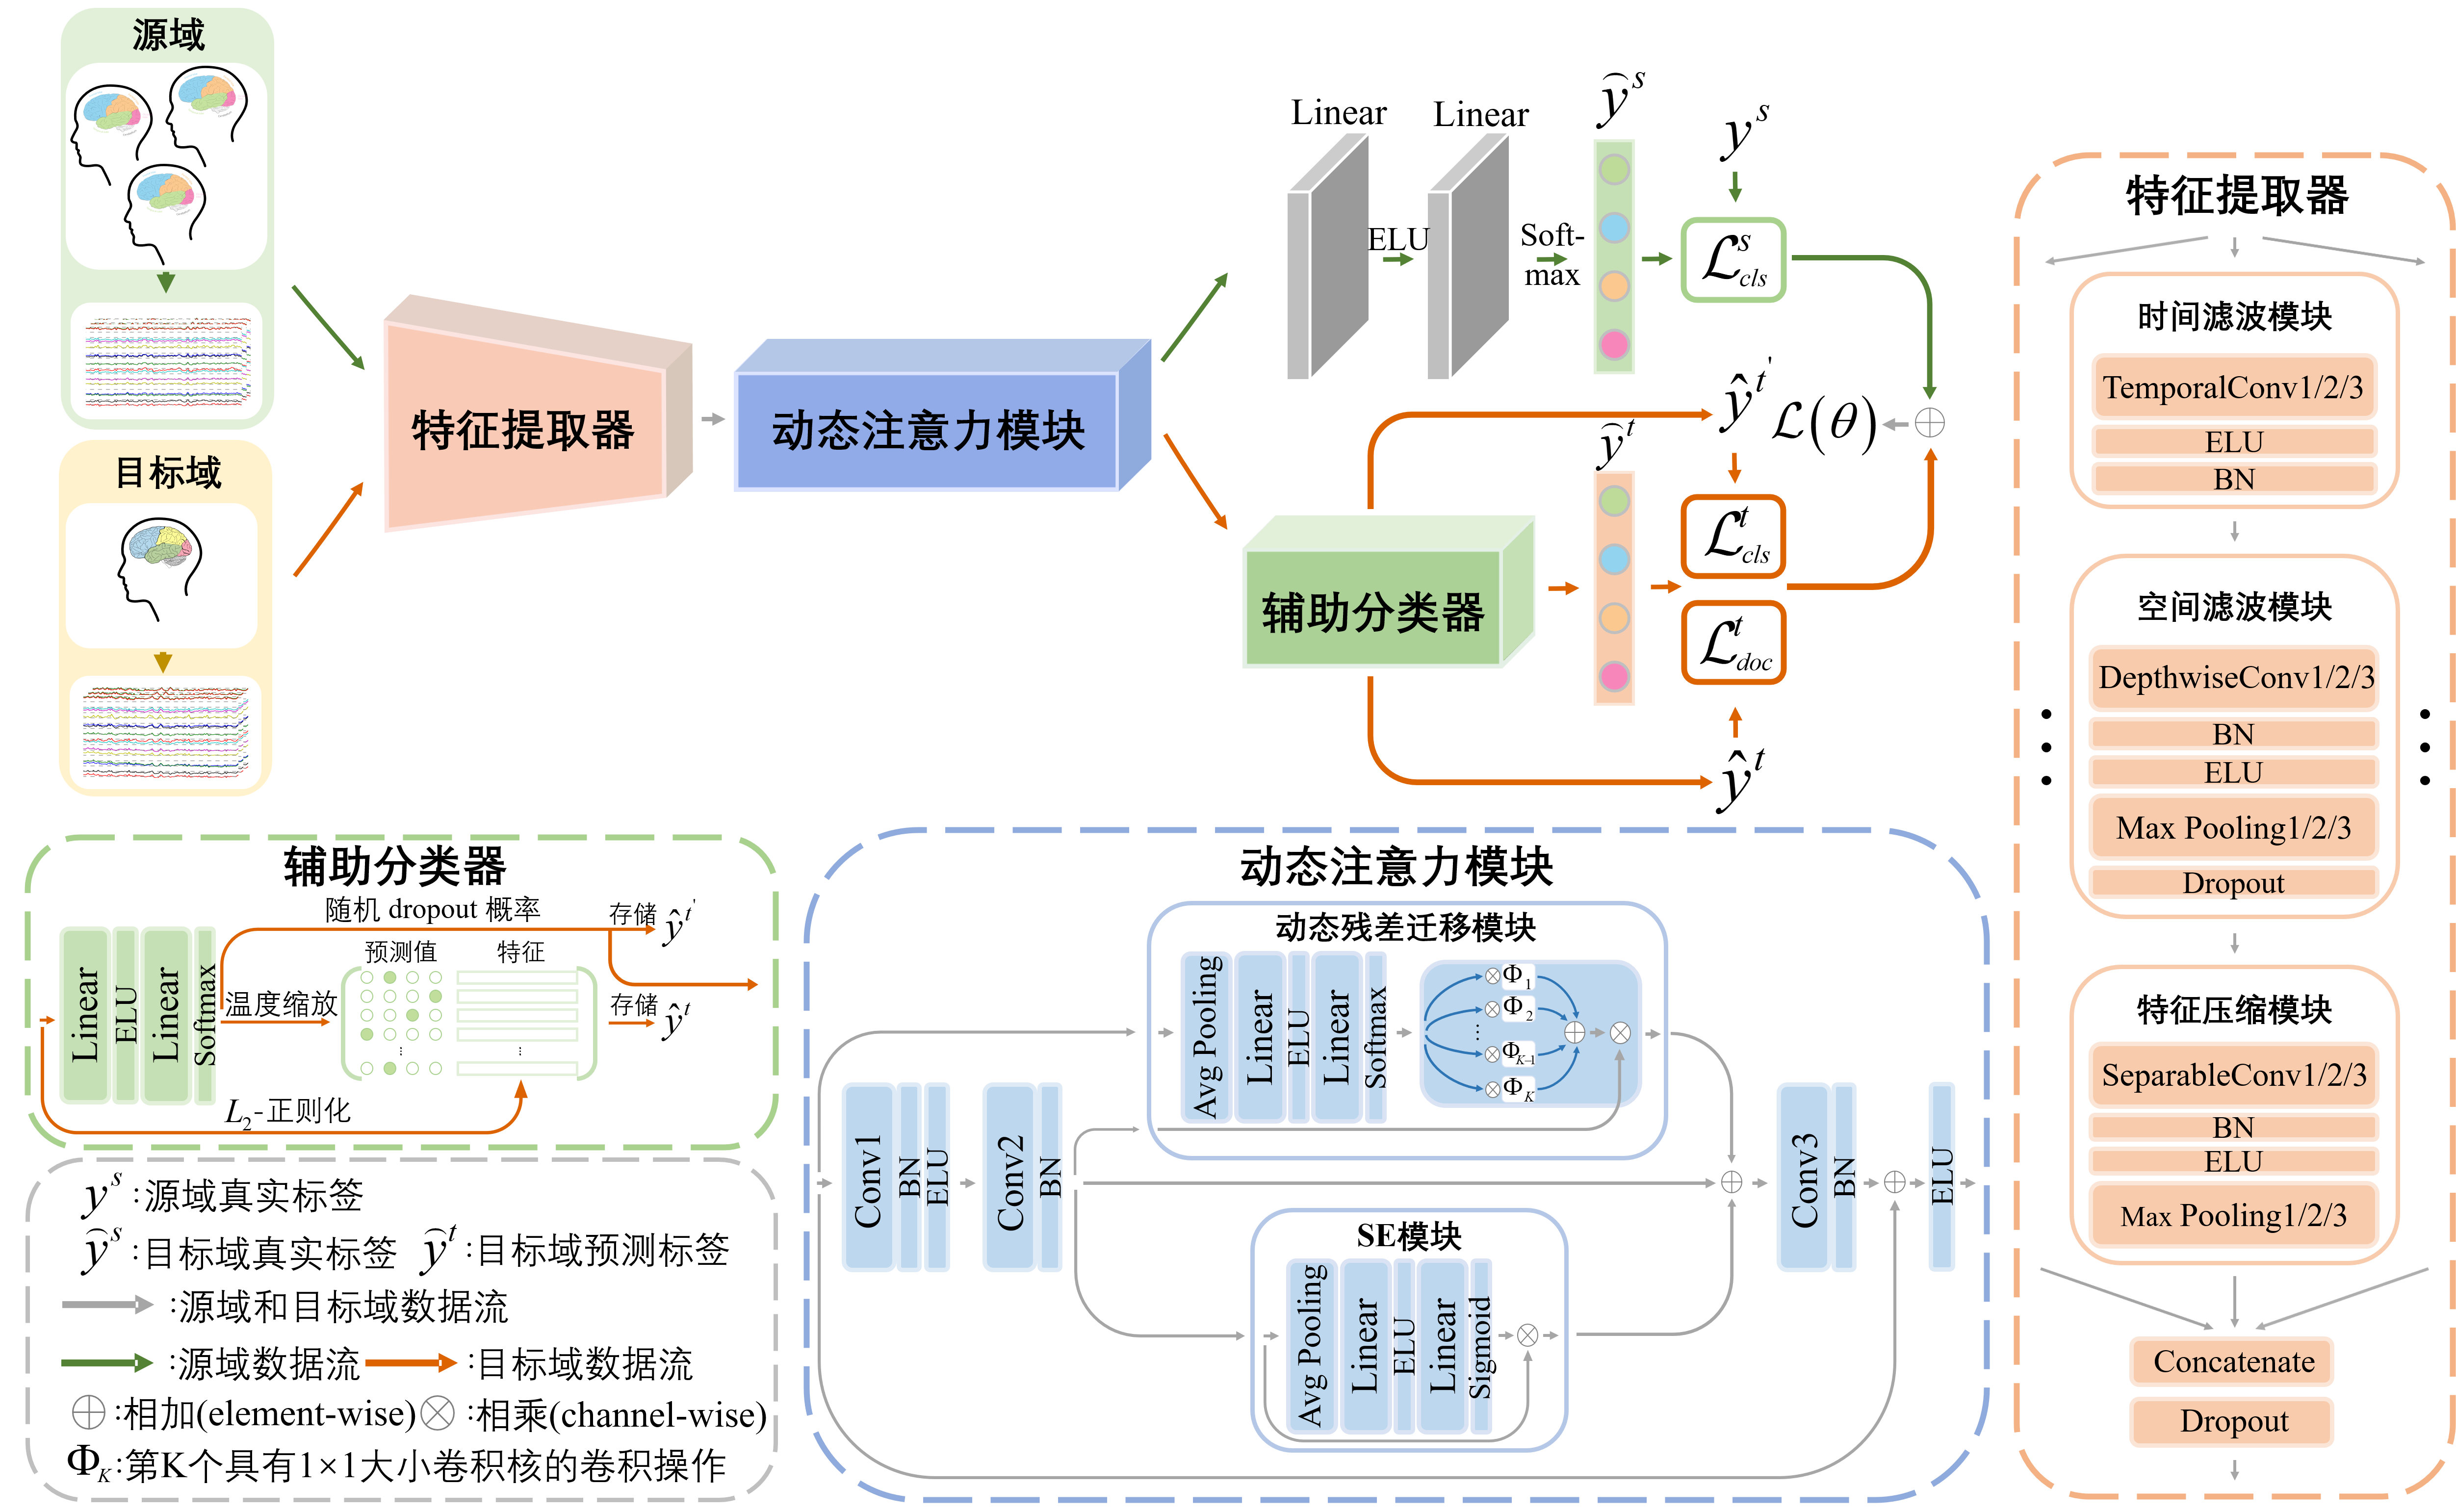
\includegraphics[width=1\textwidth]{主模型图_v1.png}
\caption{迭代自训练多被试域适模型示意图}
\label{fig_4_1}
\end{figure*}

\subsection{问题定义}
本章利用域适应算法实现MI-BCI系统的跨被试同时跨时段分类辨识,为了问题描述的准确性,在这里进行详细的问题定义。

(1) 定义和符号

设$D_{s_{j}}=\left\{\left(x_{i}^{s_{j}}, y_{i}^{s_{j}}\right)\right\}_{i=1}^{n^{s_{j}}}, j \in\{1, \ldots, N\}$代表拥有${n^{s_{j}}}$个有标签样本的$N$个源域中的第$j$个域。其中的第$i$个样本$x_{i}^{s_{j}} \in \mathbb{R}^{C \times L}$拥有$C$个通道和$L$个样本点,${y_{i}^{s_{j}}}$为第$i$个样本所对应的真实标签。${n^{s_{j}}}$代表源域$S_{j}$中所包含的EEG样本数。相似的,将包含${n^{t}}$个未标记样本的目标域$\mathcal{T}$定义为$D_{t}=\left\{\left(x_{i}^{t}\right)\right\}_{i=1}^{n^{t}}$。所有域中的样本均包含$N_{c}$个不同的类别。

考虑到不同域之间的分布差异$P_{S}\left(D_{s}\right) \neq P_{\mathcal{T}}\left(D_{t}\right)$,从不同域提取到的数据联合分布$P$需要进行对齐。假设存在一个由参数$\theta$组成的模型$M_{\theta}$,其能够减少不同域分布之间的差异,并正确地将目标域样本$x_{i}^{t}$映射到相应的类别,那么这一模型便能够解决本章所针对的问题。因此,本章所涉及的分类任务的最终目的,就是找到一个满足这一要求的模型。

(2) 基于MI-BCI系统的多被试迁移任务

本章节所进行的所有实验均满足本节中所设定的迁移学习场景,具体内容如下:选取MI数据集中某一特定被试的EEG信号作为目标域$\mathcal{T}$,其余的其他被试作为源域$\mathcal{S}=\left\{\mathcal{S}_{1}, \ldots, \mathcal{S}_{N}\right\}$,二者共同对分类器完成校准。为了进一步提高模型的实用性,设定源域数据无法携带它们的域标签,这意味着来自不同被试的数据将被随机混合并作为一个统一的源域使用。遵循Choi给出的定义\cite{4-1},本文的应用场景被定义为多被试迁移(Multi-subject Transfer)任务。

\subsection{模型结构}
本章节将从ISMDA的三大组成部分:多通道时空滤波特征提取器(MTSF),动态注意力模块(DAM)以及基于面向域分类器的迭代自训练(DCIS)分别展开介绍。

(1) 多通道时空滤波特征提取器

鉴别性特征的提取有助于提高模型下游的EEG信号辨识准确性,并且决定了模型的性能基线。本文受到EEGNet\cite{4-2}——一个成功的、可推广的EEG分类模型的启发,提出了MTSF模块。MTSF模块由三个分支组成,每个分支针对EEG信号的特点分为三个级联模块,即时间滤波模块、空间滤波模块和特征压缩模块。

\begin{table}[h]
	\caption{多通道时空滤波模块的结构参数 \label{tab4-1}}
	\centering
	\wuhao{
        \setlength{\tabcolsep}{2mm}{
		\begin{tabular}{cccc}
		  \toprule
            \textbf{模块}                      & \textbf{网络层} &\textbf{参数} & \textbf{输出} \\
            \midrule
            \textbf{输入}                       & -      &  -  & $(1, \mathrm{C}, \mathrm{L})$\\
            \midrule
            \multirow{3}*{时间滤波模块}  & TemporalConv1/2/3 & $1\times18$ / $1\times24$ / $1\times36$ $@$$F_{1}$ & $(F_{1}, C, L)$\\
                                       & $ELU$                      & & $(F_{1}, C, L)$\\ 
                                       & $BN$      & & $(F_{1}, C, L)$\\ 
            \midrule
            \multirow{5}*{空间滤波模块}  & DepthwiseConv1/2/3 & $C \times 1$$@$$F_{1}*D$, padding=`VALID'& $(F_{1}*D, 1, L)$\\
             & $BN$      &  & $(F_{1}*D, 1, L)$   \\ 
             & $ELU$                      &  & $(F_{1}*D, 1, L)$       \\ 
             & Max Pooling1/2/3         & stride=$(1, 8)$  & $(F_{1}*D, 1, L//8)$ \\ 
             & Dropout                  &  & $(F_{1}*D, 1, L//8)$          \\
            \midrule
            \multirow{6}*{特征压缩模块}   & SeparableConv1/2/3 & $1 \times 16$$@$$F_{2}$& $(F_{2}, 1, L//8)$\\
             & $BN$      & & $(F_{2}, 1, L//8)$\\ 
             & $ELU$                     & & $(F_{2}, 1, L//8)$    \\ 
             & Max Pooling1/2/3         & stride=$(1, 8)$ & $(F_{2}, 1, L//64)$   \\ 
             & Concatenate              &   & $(F_{2}*3, 1, L//64)$          \\ 
             & Dropout                  &   & $(F_{2}*3, 1, L//64)$          \\ 
             \bottomrule
    
       \end{tabular}
       }}
\end{table}


1) 时间滤波模块:在时间滤波模块中,特征提取器的三个分支首先对EEG信号进行时间卷积(Temporal Convolution)。具体来说,特征提取器的三个分支可以被看作是具有不同参数的时间滤波器,其卷积核大小分别为(1,36)、(1,24)与(1,18),滤波器数量为$F_1$。这三个分支首先采用指数线性单元(Exponential Linear Unit,$ELU$)来激活经过时间滤波的EEG特征图,以使模型获得足够的非线性表征能力。在$ELU$之后,对特征图进行批归一化操作(Batch Normalization, $BN$)。

2) 空间滤波模块:在空间滤波模块中,首先利用大小为($C$,1)的深度卷积(Depth-wise Convolution)对时间滤波模块输出的特征图进行空间滤波。对时间滤波模块输出的每个特征图,深度卷积均训练$D$个滤波器,这意味着每个深度卷积都由$F_1*D$个滤波器组成。其次,采用批归一化操作和$ELU$激活函数对空间特征图进行进一步处理。紧接着,应用大小为(1,8)的最大池化层(Max Pooling)以扩展模型的感受野。最后,引入概率为0.5的Dropout层以提高数据表示的稀疏性,减少冗余。

3) 特征压缩模块:为了在有限的计算资源中提取更加抽象化的特征,特征压缩模块采用了可分离卷积(Separable Convolution)来处理空间滤波器的输出。可分离卷积的卷积核大小和滤波器数量分别为(1,16)和$F_2$($F_2$的大小被设定为$F_1*D$)。之后,为了减少特征图的维度,引入大小为(1,8)的最大池化层。在本文中,$F_{1}$被设定为8,$D$被设定为2,$C$由数据集决定。

三个分支的输出特征将被串联(Concatenate)并扩展成一个一维向量,它以0.5的概率通过Dropout层传递给动态注意力模块。MTSF的具体参数和输出维度见表\ref{tab4-1}。

(2) 动态注意力模块

模型$M_{\theta}$被称为静态或动态,取决于其参数$\theta$是否随输入样本$x$而变化,即$\theta=\theta(x)$并且$x\in S \bigcup \mathcal{T}$。当$M_{\theta}$为动态模型时,其可以根据不同输入的特点动态地调整参数$\theta$。此时$\theta$不再需要关联于域,而是直接关联于样本。更进一步,由于模型能够直接根据样本特点实现参数调整,此时源域便不再需要与目标域进行对齐,即不同域之间不再具有固定的边界。此外,由于不再有对域信息的依赖,此时的训练过程不需要区分不同的源域,也不再需要引入域标签,这有效地降低了训练的复杂度。综上所述,在下文的描述中,源域均使用$S$来表示。

受Li等人\cite{4-3}所提出的动态残差迁移模型的启发,DAM被引入ISMDA中。此外,根据Li等人\cite{4-3}的研究,动态迁移模型可以简单地通过聚合静态矩阵和残差模块来实现,因此本章所设计的DAM模型由静态模块和动态残差模块两部分组成:
\begin{equation}
\label{deqn_ex1}
W(x)=W_{0}+\Delta {W}({x}),
\end{equation}
其中$W_{0}$代表由静态卷积矩阵组成的静态模块,$\Delta {W}({x})$代表由动态残差矩阵组成的动态残差模块。动态残差矩阵由一组通道注意力模块和子空间路由模块构成:
\begin{equation}
\label{deqn_ex2}
\Delta {W}({x})={\Lambda}({x}) {W}_{0}+\sum_{i=1}^{K} \pi_{i}(x){\Phi}_{i}.
\end{equation}

${\Lambda}({x}) {W}_{0}$代表了通道注意力模块,而${\Lambda}({x})$是一个大小为$C_{\text {out }} \times C_{\text {out }}$的对角矩阵,其中$C_{\text {out }}$代表了输出特征图的通道数量。在本章中,通道注意力模块由Squeeze-and-Excitation模块实现\cite{4-4}。

子空间路由模块$\sum_{i=1}^{K} \pi_{i}(x){\Phi}_{i}$是$K$($K=4$)个静态矩阵${\Phi}_{i}$的线性组合,其权重由输入$x$所决定。模型权重空间中的投影由动态参数$\pi_{i}(x)$和静态矩阵${\Phi}_{i}$的乘积来选择,这本质上是选择不同的子空间来路由不同的输入$x$。动态参数由一个平均池化(Average Pooling)层和两个全连接(Linear)层组成的注意力分支所产生。在本文中,采用$softmax$对${\Phi}_{i}$进行归一化。

如图\ref{fig_4_1}所示,受ResNet中瓶颈结构的启发,特征提取器输出的特征通道数首先通过一组相继连接的卷积层、批归一化层和$ELU$激活函数转换为48,然后进入DAM。在通道注意力模块和子空间路由模块之后,特征向量将被拼接,特征向量的通道数通过一组卷积层和批量归一化层被扩展到原先的四倍。最后,经由残差连接,DAM的输出传递给下一模块。

(3) 基于面向域分类器的迭代自训练

为了削弱分布偏移所带来的影响,避免模型过于偏向源域数据,本节引入了一种新的伪标签训练策略——DCIS。DCIS包含ATDOC和PACC两种伪标签算法,以迭代自训练的方式分两个阶段分别引入模型的训练过程中。两个阶段均采用了相同数量的epochs以保证模型的最终性能。

1) 面向域分类器:考虑到基于邻域聚合的ATDOC模型显著优于已有的域对齐技术和半监督学习算法\cite{4-5},本节采用其作为DCIS中的第一种伪标签生成策略。鉴于目标域的标签稀疏性,one-hot伪标签由下式得到\cite{4-6}:
\begin{equation}
\label{deqn_ex3}
\hat{y}^{t}=\arg \max _{k} p_{k}^{t},
\end{equation}
其中$p^{t}$是输入$x^{t}$的预测结果,为$N_{C}$维向量。利用MTSF和DAM提取的特征,经由一组全连接层组成的分类器即可获得$p^{t}$。

在本文中,为了防止预测中可能出现的混淆问题,首先利用$a=0.5$的温度缩放(Temperature Scaling)\cite{4-7}对预测结果$p^{t}$进行锐化:
\begin{equation}
\label{deqn_ex4}
{\check{p}_{k}^{t}}=(p_{k}^{t})_{{}}^{\frac{1}{a}}/\sum\nolimits_{k=1}^{{{N}_{c}}}{(p_{k}^{t})_{{}}^{\frac{1}{a}}}.
\end{equation}
从上式可以看出,随着$a$逐渐收敛为零,预测值$p^{t}$将从概率分布坍缩到一个特定的点,即某一具体类别。之后,当前目标域样本的锐化预测值${\check{p}_{k}^{t}}$将与它对应的$L_{2}$正则化特征向量
\begin{equation}
\label{deqn_ex5}
f^{t'}=f^{t} /\left\|f^{t}\right\|_{2}
\end{equation}
根据其在数据集中的索引位置,一起被存储在一个独立的模块中,即记忆库(Memory Bank)。其中$f^{t}$是由DAM输出得到的特征向量。在每一批目标域样本通过模型后,新的样本将被添加到记忆库中。

按照邻域聚合策略,利用余弦相似度检索出与每个样本特征向量最接近的$m$($m=5$)个其他样本。然后,通过对最接近的$m$个样本的预测值进行平均,得到当前样本的伪标签:
\begin{equation}
\label{deqn_ex6}
{\hat{q}_{k}^{t}}=\frac{1}{m}\sum\nolimits_{j\in {{\mathcal{N}}_{i}}}\check{p}_{j,k}^{t},
\end{equation}
其中${\mathcal{N}}_{i}$代表了记忆库中所有样本所携带的索引集。在完成所有样本的迭代后,记忆库将建立一个反映目标域全局结构的分类器,而无需学习任何新的参数。

由面向域分类器得到的目标域样本的伪标签为:
\begin{equation}
\label{deqn_ex7}
\hat{y}^{t}=\arg \max _{k} \hat{q}_{k}^{t}.
\end{equation}

然而,位于密度较高邻域的样本具有较高的正确分类概率,这可以直接反映在${\hat{q}}^{t}$中最大子项的数值大小上。因此,采用${\hat{q}}^{t}$作为伪标签的置信度权重,得到目标域样本的面向域分类器交叉熵损失:
\begin{equation}
\label{deqn_ex8}
\min{\mathcal{L}_{doc}^{t}=-\mathbb{E}_{x^{t}\sim P_\mathcal{T}}\sum\nolimits_{k=1}^{N_c}{\mathbbm{1}_{\left[{\hat{y}}^{t}=k\right]}{\hat{q}}_k^{t} \log {p_k^{t}}}}.
\end{equation}

2) 迭代自训练:在ATDOC之外,DCIS还建立了一个由两个顺序连接的全连接层组成的分类器。由MTSF和DAM输出的特征将首先被扩展成为一维向量,并传递给具有500个单元的第一个全连接层,如图\ref{fig_4_1}所示。这个全连接层采用$ELU$作为激活函数。接下来,拥有$N_C$个单元的第二个全连接层采用$softmax$激活函数来获得最终的分类结果。

根据常见的自训练策略,所有的目标域样本都必须事先进行伪标签化。然而在一定程度的训练之前,网络无法对目标域的样本进行正确的分类。综上所述,本文引入了迭代式自训练策略。在迭代式自训练的第一阶段,首先使用ATDOC生成伪标签来训练网络。在第二阶段,ATDOC将被冻结,从第一阶段得到的经过完善训练的模型所产生的新伪标签$\hat{y}^{t^{'}}$,将被用来对当前模型进行进一步微调。在这一时刻,虽然模型具有足够的分类精度,但其不一定经过足够的校准,即模型的$softmax$输出可能并不是决策置信度的真实反映\cite{4-7}。具体来说,此时的伪标签中混入了大量高置信度的错误分类结果,此时将这种充满噪声的标签引入未经校准的模型毫无疑问是灾难性的。考虑到置信度和确定性问题,迭代式自训练的第二阶段的伪标签是:
\begin{equation}
\label{deqn_ex9_addation1}
\hat{p}_{k}^{t^{'}} = \left\{\begin{array}{cl}
\overline{p}_{k}^{t},&\text{if}\ {u}({p}_{k}^{t,i}) \leq {k}_{u}\ \text{and}\ \ \overline{p}_{k}^{t} \geq {k}_{c}\\ 
discard,&{\text{otherwise}}
\end{array}\right.,
\end{equation}
其中$i=1,2,\cdots,U$。在第一阶段得到的模型基础上,随机设置其Dropout概率$U$次,并对同一样本进行$U$次预测以获得一组${p}_{k}^{t,i}$。$\overline{p}_{k}^{t}$代表了$U$个${p}_{k}^{t,i}$的平均值。$\overline{p}_{k}^t$可以被看做是伪标签置信度的评价指标,这源于一个事实,即每个具有不同Dropout概率的模型可以被视为具有不同参数的子模型,众多子模型的联合投票结果将会更为鲁棒与可信。同时,受预期校准误差(Expected Calibration Error)\cite{4-7}和模型不确定性(Model Uncertainty)之间的相关性启发\cite{4-9},同一样本在不同预测值${u}({p}_{k}^{t})$上的置信度方差被视为不确定性的评价指标。最终,满足置信度与不确定性指标的$\overline{p}_{k}^t$,即方差低于阈值${k}_{u}$而均值高于阈值${k}_{c}$的伪标签,将会在第二阶段得以保留。不符合要求的标签将被直接舍弃。
\begin{equation}
\label{deqn_ex9_addation2}
\hat{y}^{t^{'}} = \arg \max _{k} (\hat{p}_{k}^{t^{'}}).
\end{equation}

此外,鉴于容易区分的类别会有更多的样本符合阈值条件,因此本章节引入了一个样本平衡策略,以避免模型在训练过程中产生对于某类样本的偏向性。具体来说,通过计算所有符合条件的样本并依次保留具有高置信度和低不确定性者,使每个类别的样本数量保持一致。在第二阶段,伪标签经过每100个epoch将被更新一次,以保证伪标签的可靠性随着训练进程而逐步提高。第二阶段的自训练交叉熵损失如下:
\begin{equation}
\label{deqn_ex9}
\min{\mathcal{L}_{cls}^t=-\mathbb{E}_{x^t\sim P_\mathcal{T}}\sum\nolimits_{k=1}^{N_c}{\mathbbm{1}_{\left[{\hat{y}}^{t^{'}}=k\right]} {\log {p_k^t}}}}. 
\end{equation}

为了避免可能出现的不确定性,在本章节中,设定$U$为30,设定${k}_{u}$为0.05,设定${k}_{c}$为0.7。

\begin{algorithm}[!h]
\algsetup{linenosize=\small}
\small
\setcounter{algorithm}{0}
\floatname{algorithm}{\small{算法4 -}} 
\caption{\small{ISMDA的算法流程.}}\label{alg:alg1}
\begin{algorithmic}
\STATE 
\STATE{\textbf{输入:}}\ 源域的EEG时间序列以及对应标签: $ D_{s}=\left\{\left(x_{i}^{s}, y_{i}^{s}\right)\right\}_{i=1}^{n^{s}}$;
\vspace{0.22cm}
\STATE \hspace{0.90cm}\ 目标域的EEG时间序列: $ D_{t}=\left\{\left(x_{i}^{t}\right)\right\}_{i=1}^{n^{t}}$;
\vspace{0.22cm}
\STATE \hspace{0.90cm}\ DCIS中的近邻样本数: $m$;
\vspace{0.22cm}
\STATE \hspace{0.90cm}\ 模型$M$的学习率: $\eta$;
\vspace{0.22cm}
\STATE \hspace{0.90cm}\ 源域与目标域数据的batch size: $n$;
\vspace{0.22cm}
\STATE \hspace{0.90cm}\ 单个训练阶段的epoch数:  $E$.
\vspace{0.22cm}
\STATE{\textbf{输出:}}\ 训练后的模型参数: $\Theta$.
\vspace{0.22cm}
\STATE{\textbf{初始化:}}\ 初始模型参数:  $\Theta$;
\vspace{0.22cm}
\STATE \hspace{1.3cm}\ 计算公式(\ref{eq:12B})中权重$\lambda$的初始值: $\frac{1}{n^{s} \times E}$;
\vspace{0.22cm}
\STATE \hspace{1.3cm}\ 记忆库初始化. 
\vspace{0.22cm}
\STATE 1. \textbf{For} \textbf{训练阶段}$\in[1,2]$ \textbf{do}:
\vspace{0.22cm}
\STATE 2. \hspace{0.4cm}根据公式(\ref{eq:12})更新调节参数 $\alpha(T), \beta(T), \gamma(T)$;
\vspace{0.22cm}
\STATE 3. \hspace{0.4cm}\textbf{For} $T \in[1, E]$ \textbf{do}:
\vspace{0.22cm}
\STATE 4. \hspace{0.8cm}当\textbf{训练阶段}等于2并且\textbf{$T$}被100整除时,利用公式(\ref{deqn_ex9_addation1})生成目标域伪
\vspace{0.22cm}
\STATE \hspace{1.16cm} 标签:$M$: $\left\{\hat{y}_{i}^{t}\right\}_{i=1}^{n_{t}} \leftarrow \Theta, D_{t}^{\prime}=D_{t} \cup\left\{\hat{y}_{i}^{t}\right\}_{i=1}^{n_{t}}$;
\vspace{0.22cm}
\STATE 5. \hspace{0.8cm}从源域$D_{S}$中取出一个batch的源域样本$\left\{\left(x_{i}^{s},y_{i}^{s}\right)\right\}_{i=1}^{n}$;
\vspace{0.22cm}
\STATE 6. \hspace{0.8cm}从目标域$D_{t}^{\prime}$中取出一个batch的目标域样本$\left\{\left(x_{i}^{t},\hat{y}_{i}^{t}\right)\right\}_{i=1}^{n}$;
\vspace{0.22cm}
\STATE 7. \hspace{0.8cm}\textbf{For} \textbf{样本} $\in$ batch \textbf{do}:
\vspace{0.22cm}
\STATE 8. \hspace{1.2cm}更新公式(\ref{eq:12B})中的权重$\lambda$;
\vspace{0.22cm}
\STATE 9. \hspace{1.2cm}利用公式(\ref{deqn_ex10})计算源域有监督损失$\mathcal{L}_{cls}^{s}$;
\vspace{0.22cm}
\STATE 10.\hspace{1.15cm}计算邻域聚合伪标签$\hat{q}^{t}$;
\vspace{0.22cm}
\STATE 11.\hspace{1.15cm}根据公式(\ref{deqn_ex8})和公式(\ref{deqn_ex9})计算目标域无监督损失$\mathcal{L}_{d o c}^{t}$和$\mathcal{L}_{c l s}^{t}$;
\vspace{0.22cm}
\STATE 12.\hspace{1.15cm}根据公式(\ref{deqn_ex11})计算整体损失$\mathcal{L}(\theta)$;
\vspace{0.22cm}
\STATE 13.\hspace{1.15cm}优化模型参数: $\Theta \leftarrow \Theta-\mu \frac{\partial \mathcal{L}}{\partial \Theta}$;
\vspace{0.22cm}
\STATE 14.\hspace{1.15cm}更新记忆库;
\vspace{0.22cm}
\STATE 15. {\textbf{结束}};
\vspace{0.22cm}
\STATE 16. 返回训练好的模型参数$\Theta$;
\end{algorithmic}
\end{algorithm}

(4) 网络优化框架

由MTSF、DAM和DCIS组成的ISMDA框架,利用基于源域数据的有监督学习和基于目标域数据的自训练策略在两个迭代的训练阶段进行逐步优化。ISMDA的整个训练流程详见算法4 -\ref{alg:alg1}。具体来说,$M_\theta$的参数可以通过同时最小化源域中的有监督学习损失和目标域中的自训练损失来完成优化。考虑到源域和目标域之间数据量的差异性,采用带有标签平滑正则化(Label-Smoothing Regularization)\cite{4-8}的交叉熵损失作为源域的损失函数:
\begin{equation}
\label{deqn_ex10}
\min\mathcal{L}_{cls}^{s}=-\mathbb{E}_{\left(x^{s}, y^{s}\right) \sim P_{s}} \sum\nolimits_{k=1}^{N_{c}} q_{k}^{\prime} \log {p_k^s},
\end{equation}
其中$p_k^s$是源域样本$x^{s}$的预测值的第$k$维,$q^{\prime}$是经过标签平滑后的one-hot真实标签。基于上述描述,ISMDA的整体损失函数可以表征为:
\begin{equation}
\label{deqn_ex11}
\mathcal{L}(\theta)=\alpha(T) \mathcal{L}_{c l s}^{s}+\beta(T) \mathcal{L}_{d o c}^{t}+\gamma(T)\mathcal{L}_{cls}^{t}
\end{equation}
其中$\alpha(T)$,$\beta(T)$,$\gamma(T)$是被用来在训练进程$T$中平衡有监督学习和自训练的调节参数。为了获得模型的最佳性能,在不同的训练阶段采用了不同的参数值:
\vspace{-2mm}
\begin{subequations}
\label{eq:12}
\begin{align}
\alpha(T) =& \left\{\begin{array}{rll}
\alpha_{0},&T\leq E&\\
0.1\times\alpha_{0},&E<T\leq 2E,&
\end{array}\right.\label{eq:12A}\\[1.5mm] 
\beta(T) =& \left\{\begin{array}{rll}
\ \ \lambda \times \beta_{0} ,&T \leq E&\\
0 ,&E<T \leq 2E,&
\end{array}\right.\label{eq:12B}\\[1.5mm]
\gamma(T) =& \left\{\begin{array}{rll}
\ \ \ \ \ \ \ \ \ 0 ,&T\leq E& \\
\gamma_{0} ,&E<T \leq 2E,&
\end{array}\right.\label{eq:12C}
\end{align}
\end{subequations}
考虑到记忆库在训练的第一阶段开始时,仅仅只能获取较为粗略的原始特征向量,权重$\lambda$采用了线性缩放策略(Linearly Scheduling Skill)以保证ATDOC在初始时不会对模型产生较大影响。而随着记忆库中鉴别性表征的增加,$\lambda$以$\frac{1}{n^{t} \times E}$为步长,逐渐从$\frac{1}{n^{t} \times E}$增长到1。$E$代表了一个训练阶段所需要进行的epoch数。$\alpha_{0}$,$\beta_{0}$,$\gamma_{0}$在BCI IV IIa Dataset和JS-MI Dataset上被设定为1,0.2,2,而在High Gamma Dataset和Additional Dataset上$\alpha_{0}$,$\beta_{0}$,$\gamma_{0}$被设定为1,0.02,2。 值得注意的是,$\mathcal{L}_{c l s}^{s}$的权重$\alpha_{0}$在第二个训练阶段被乘以了一个缩放系数,其大小为0.1。




\section{实验描述}
本章详细介绍了对比试验所引入的四种数据集和八种对比方法,并描述了对比实验的具体流程与参数设计。

\subsection{运动想象数据集}
为了评估本章所提出的基于多被试动态迁移与迭代自训练的EEG辨识算法的有效性,并进一步考量JS-AINS-40设备的实际使用效果。本章引入了三个公开的MI-EEG数据集与一个JS-AINS-40采集的MI-EEG数据集来评估模型的性能。公开数据集包括第四次BCI竞赛中的IIa数据集(BCI IV IIa Dataset)\cite{4-10}、High Gamma Dataset (HGD)\cite{4-11}以及Kwon等人采集的数据集(Additional Dataset)\cite{4-12}。JS-AINS-40采集的MI-EEG数据集称为JS-MI Dataset。所有的数据集都捕捉到了人脑的电生理活动,这些活动在特定的频段上与外部刺激的反应相吻合。

(1) 数据集I:BCI IV IIa Dataset

BCI IV IIa Dataset以250 Hz的采样率在两个时段中利用22个EEG电极和3个眼电电极记录了9名不同受试者的MI信号。此外,其包含的两个时段是在不同日期采集的。在实验开始前,每个受试者都被告知将会进行四种类型的MI任务,包括左手、右手、脚和舌头。每个时段均包括288个4秒钟的MI实验。采集结束后,数据集作者使用0.5 Hz到100 Hz的带通滤波器与50 Hz的工频陷波滤波器对原始EEG信号进行了预处理。本章所使用的数据只包括22个EEG通道,直接舍弃了3个眼电通道。

(2) 数据集II:High Gamma Dataset

与其他MI数据集相比,High Gamma Dataset在采集过程中引入了高分辨率的放大器、电磁屏蔽和全光学去耦,获得了高质量的EEG信号。High Gamma Dataset采集了14名健康受试者的四个MI类别EEG,包括左手、右手、双脚和休息(没有运动,但与其他类别具有相同的视觉引导)。每名受试者都经由128通道电极在500 Hz采样率下采集了1040次MI实验数据。根据Schirrmeister等人\cite{4-11}的工作,在本章中High Gamma Dataset数据集被降采样为250 Hz,并且只保留其中的44个电极以去除冗余信息。

(3) 数据集III:Additional Dataset

Additional Dataset是一个二分类MI数据集,包含54名健康的受试者。在所有受试者中,38人是初次参与EEG实验,其他人则拥有EEG实验经历。每名受试者均被要求在指导下进行四个时段的左/右手MI,共400次实验,每次持续4秒。Additional Dataset使用62个EEG电极在1000 Hz采样率下完成了EEG信号采集。遵循Zhang等人\cite{4-13}的工作,数据集被降采样至250 Hz。

(4) 数据集IV:JS-MI Dataset

为验证JS-AINS-40的实际使用效果,设计全新的MI实验以对其性能进行评估。在本次实验中获得的数据集即JS-MI Dataset,实验的详细内容如下所述。

本次实验共选取了9名年龄在20-30岁之间的受试者(5名男性,4名女性),这些受试者均身体健康,无视力及大脑相关疾病,没有吸毒史,且在近几周保持了健康的作息。9名受试者中有5人曾参与EEG实验,4人不具备相关的实验经历。本实验经过了天津医科大学总医院的伦理委员会的审查,并签署了知情同意书。

为了验证的合理性,实验的整体流程在BCI IV IIa Dataset的基础上进行设计。首先,每名受试者在不同日期完成两次EEG数据采集(两个时段),每次实验均保持相同的流程。其次,实验包括四个基本类别的运动想象任务,分别为左手、右手、双脚以及舌头。四个类别在两个时段中以随机的顺序出现,每个类别均出现144次,即每名被试在两个时段中一共采集576段EEG数据。
在实验开始前,对所有受试者进行了实验内容的相关介绍,并让所有受试者保持舒适的坐姿佩戴EEG电极帽目视电脑屏幕中心,与电脑屏幕保持约70 cm的距离。在确认受试者准备就绪后,运行JS-AINS-40系统进行数据采集。

\begin{figure}[h]
	\centering
	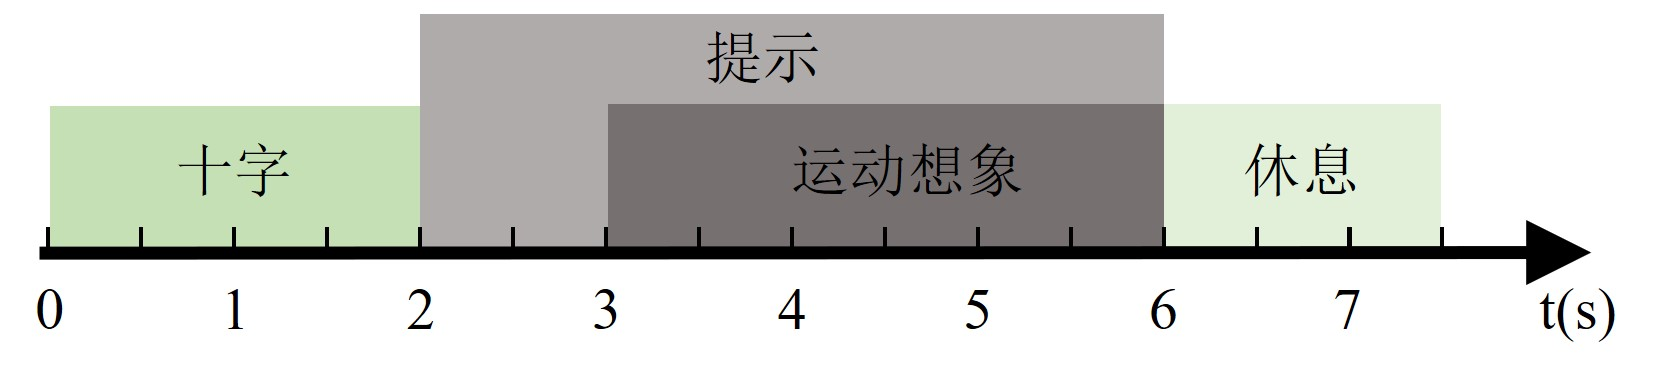
\includegraphics[width=0.5\textheight]{figures/运动想象实验流程.jpg}
	\caption{JS-MI Dataset的实验流程} 
	\label{fig_4_2}
\end{figure}

实验中,遵循图\ref{fig_4_2}完成实验流程。每次实验开始时($t=0$ s),屏幕中心会出现固定的十字以提醒受试者保持专注。在两秒后($t=2$ s),屏幕中心会出现与MI类别相对应的照片,提示受试者完成相应的想象任务,如图\ref{fig_4_3}。照片提示将会一致维持,直至本次实验结束($t=6$ s)。在照片开始显示的1秒后($t=3$ s),系统左上角将提示受试者当前应进入想象阶段,右上角则给出了当前任务的剩余时间。当想象结束后($t=6$ s),受试者将会得到1.5秒的休息。在整个实验过程中,始终开启50 Hz工频陷波滤波器对数据进行滤波。

\vspace{7mm}

\begin{figure}[h]
	\centering
	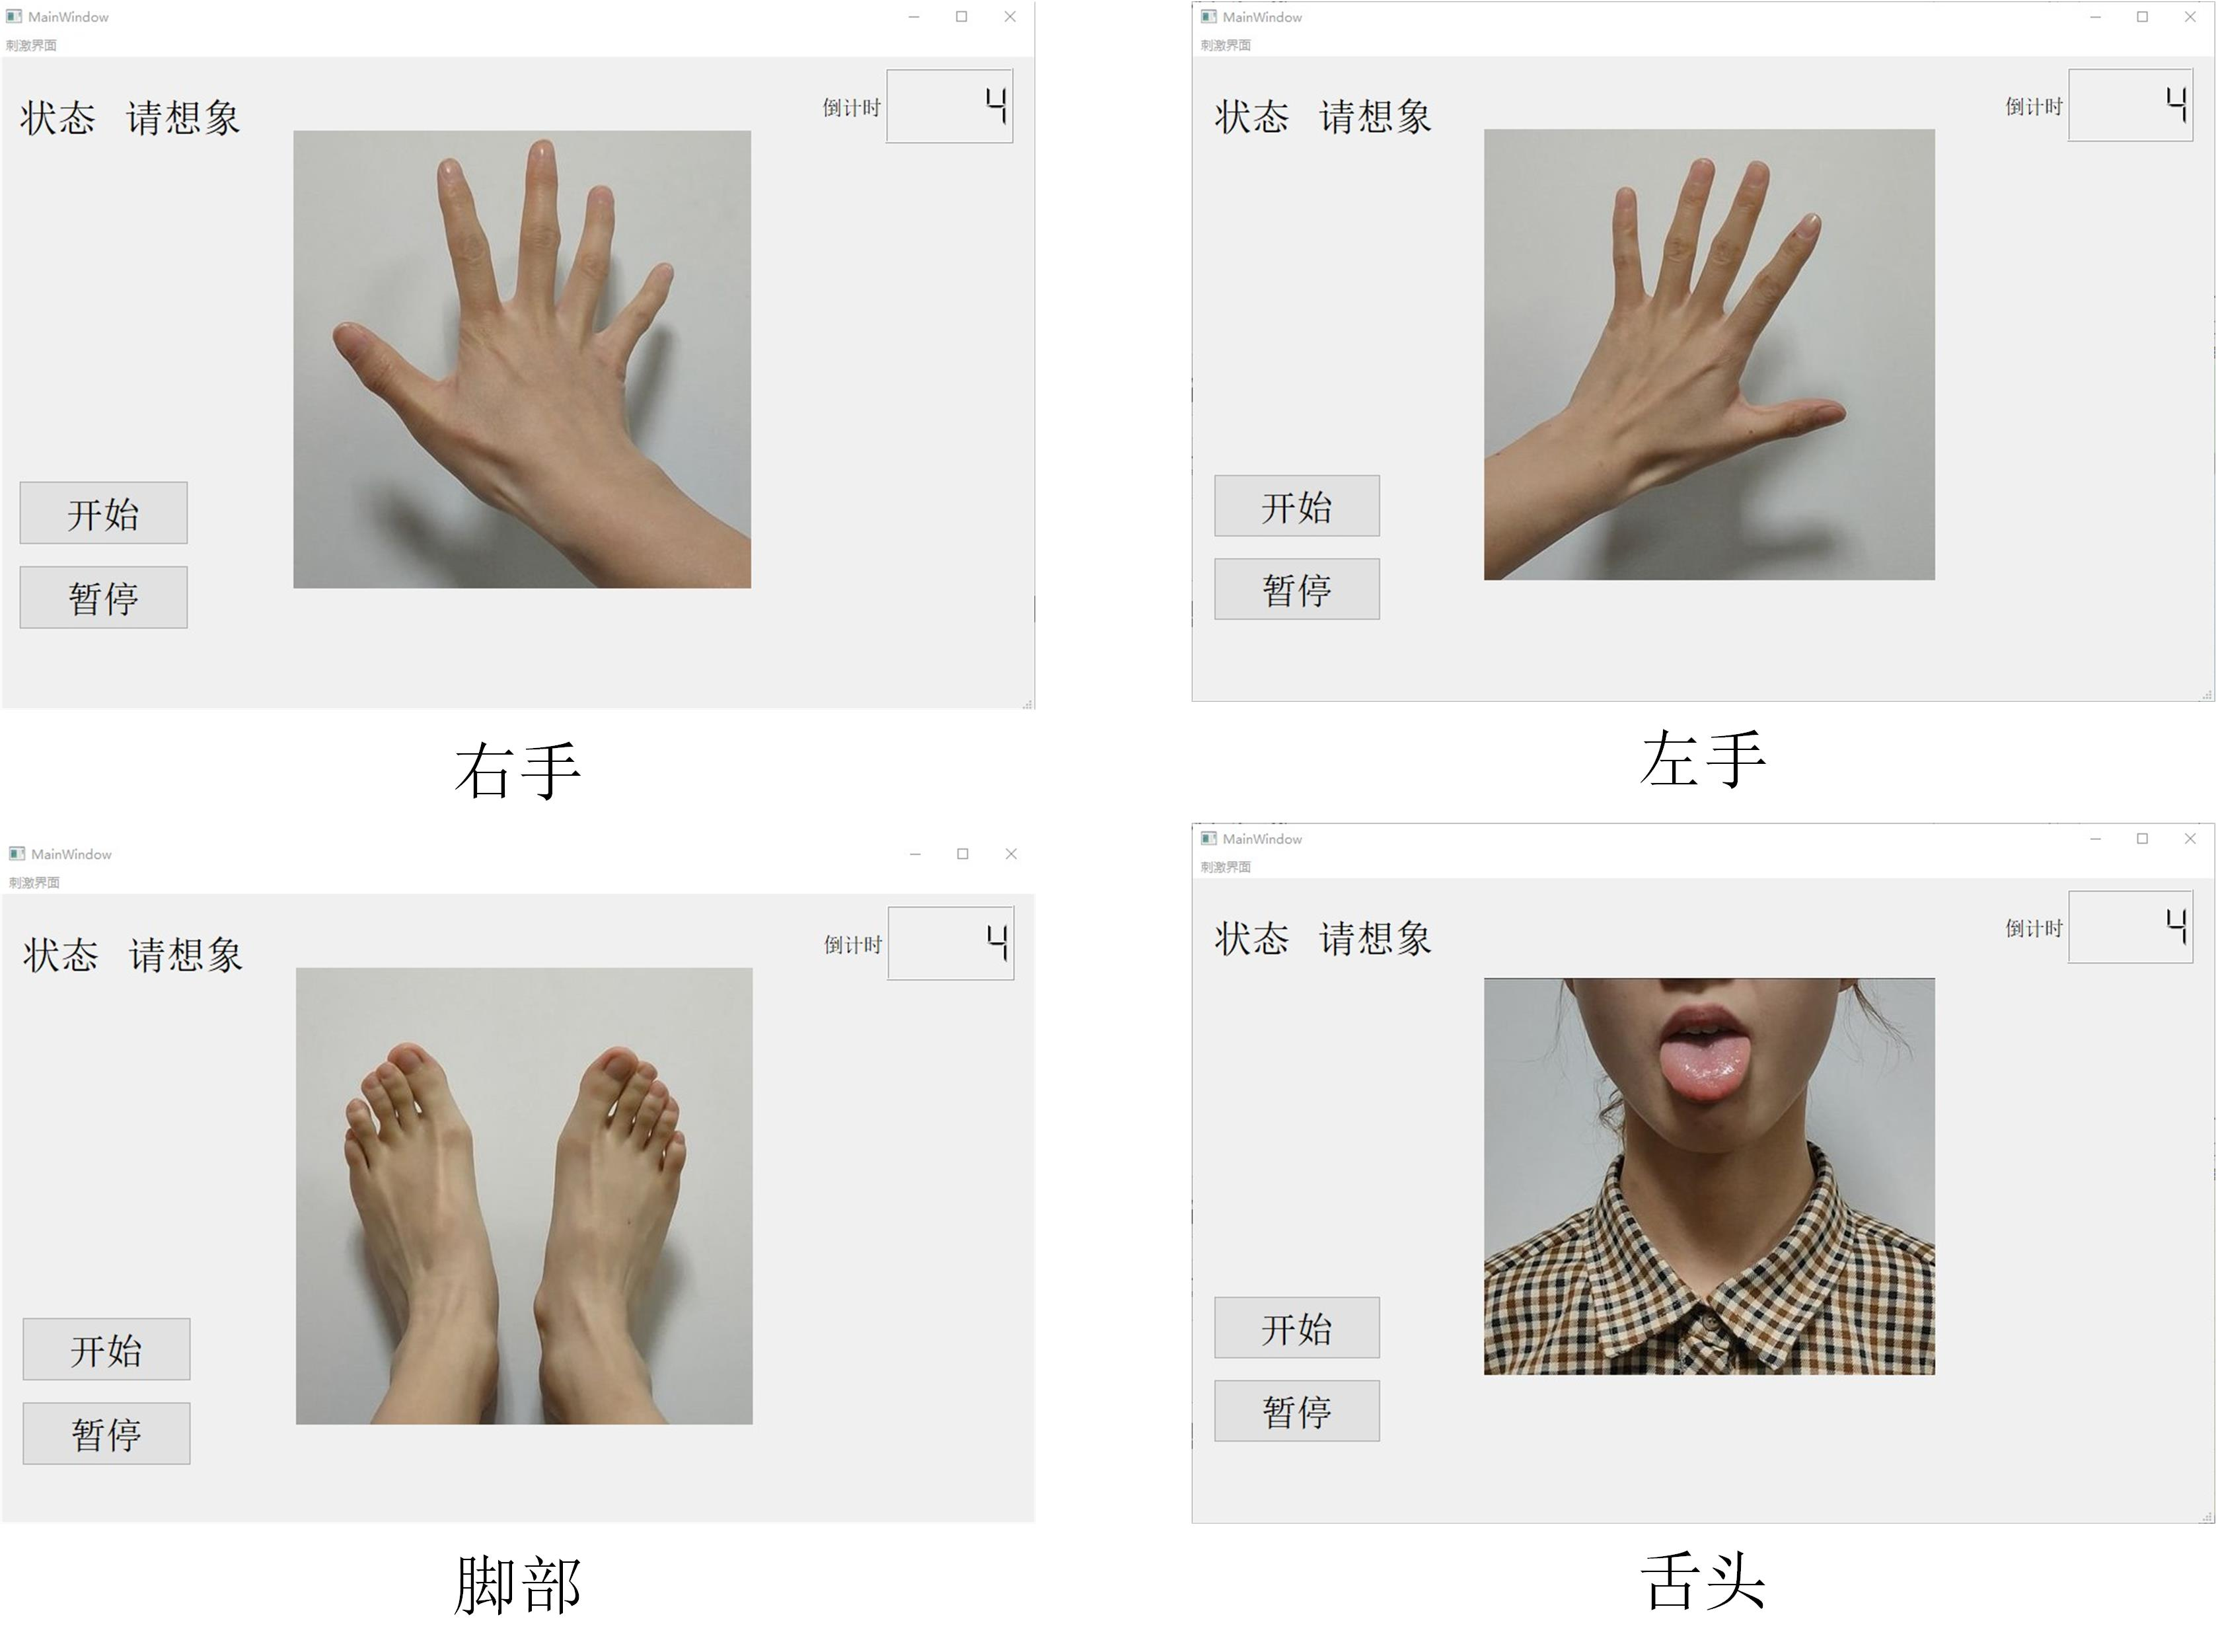
\includegraphics[width=0.57\textheight]{figures/运动想象实验.jpg}
	\caption{提示界面} 
	\label{fig_4_3}
\end{figure}

实验结束后,首先与BCI IV IIa数据集一致,进行0.5 Hz-100 Hz的带通滤波。紧接着,将数据下采样至250 Hz。为了去除可能存在的眼电干扰,使用独立分量分析\cite{4-29}对EEG数据进行处理。最后,参照Brunner等人研究\cite{4-10}中的描述,本章节仅保留JS-AINS-40的40个通道中与BCI IV IIa相同或位置相近的22个完成分类任务,具体为:Fz, FT7,FC3,FCz,FC4,FT8,T7,C3,Cz,C4,T8,TP7,CP3,CPz,CP4,TP8,P7,P3,Pz,P4,P8,Poz。

% IIA 原始通道:Fz, FC3, FC1, FCz, FC2, FC4, C5, C3, C1, Cz, C2, C4, C6, CP3, CP1, CPz, CP2, CP4, P1, Pz, P2, Poz。



\subsection{对比方法}
本文引入八种先进的算法进行结果对比,包括ShallowConvNet\cite{4-11}、EEGNet\cite{4-2}、EA-CSP\cite{4-15}、DRDA\cite{4-16}、MS-MDA\cite{4-17}、DAAN\cite{4-18}、CDAN\cite{4-19}和MCC\cite{4-20}。上述比较方法涉及机器学习算法、经典的深度学习模型和无监督域适应算法。这些算法中的大多数已经被证明可以胜任MI分类任务。考虑到本章所提出的模型属于无监督域适应的一种,上述对比方法中还包括了基于对抗策略、基于多源域和基于条件对齐的无监督域适应算法,以此证明本模型在无监督域适应领域中的先进性。

(1) ShallowConvNet(S-Conv)

一个专门为提取振荡信号中对数功率谱相关特征而设计的卷积网络结构。ShallowConvNet由连续的时间空间模块、非线性激活函数和全连接层组成。

(2) EEGNet

一个紧凑的卷积神经网络,设计了一种经典的EEG特征提取结构。深度卷积和可分离卷积的引入使其能够在不同范式的各种EEG信号上获得有竞争力的结果。在本文中,EEGNet-8,2被进行调整以适应250 Hz采样率的EEG信号。具体来说,EEGNet的第一个二维卷积核从(1,64)改为(1,125);第一个二维平均池化层从(1,4)改为(1,8)。

(3) EA-CSP

一种被广泛应用于MI-EEG场景下的迁移学习框架,它有效地结合了欧氏空间对齐和多分类CSP模型。本文引入线性判别算法(Linear Discriminant Analysis,LDA)对EA-CSP中提取的特征进行分类。

(4) DRDA

一种针对MI-EEG信号的新型端到端深度域适应方法,可以利用不同被试的判别性潜在特征提高分类性能。DRDA采用的中心损失技术可以进一步降低特征空间的非平稳性。由于其代码未公开,本文仅给出BCI IV IIa上的结果。

(5) MS-MDA

作为一种全新的迁移学习框架,MS-MDA为来自多个不同源域的EEG数据分别构建了独立的分支,用一对一的域适应方法来对齐多源域的边缘分布。由于该模型为情绪EEG设计,在本文中其通用特征提取器(Common Feature Extractor)被替换为MTSF以确保比较的公平性。同时,在MTSF和特定域特征提取器(Domain-specific Feature Extractor)之间加入了一个全连接层,以保证特征维度的一致性。

(6) DAAN

DAAN同时考虑了边缘分布(全局分布)和条件分布(局部分布)的贡献差异。它引入了动态学习来定量评估全局和局部域分布的相对重要性。使用MTSF作为DAAN的特征提取器。

(7) CDAN

CDAN是一个基于对抗的域适应方法,其将对抗学习与分类器预测中获取的鉴别性信息进行结合。在CDAN中,多线性调节(Multilinear Conditioning)被用来捕捉特征表示和分类器预测之间的交叉协方差。熵调节(Entropy Conditioning)被用来控制分类器预测的不确定性并确保模型具有足够的迁移能力。同样地,MTSF被引入作为CDAN的特征提取器。

(8) MCC

MCC提出了一个全新的损失函数,可以胜任多种迁移任务。这是一种具有快速收敛性的非对抗性域适应方法。它的性能已经在多源部分域适应(Multi-source Partial Domain Adaptation)和多目标部分域适应(Multi-target Partial Domain Adaptation)中得到了证明。这里,MTSF被用作特征提取器。

\subsection{实验设定}

由于所提出的模型是为多被试场景而设计的,使用LOSO对模型进行训练与测试。来自一个被试的数据被选为测试集(目标域),所有其他被试被视为训练集(源域)。为了充分验证模型在实际应用中的性能,本文设计了一个严苛的BCI系统使用场景,即训练数据和测试数据既不是来自同一被试,也不是来自同一时段。所有的对比方法也都遵循上述设定。值得注意的是,本文关于Additional Dataset的实验方案遵循了数据集作者所提出的“Subject-Independent”设置\cite{4-12, 4-13}。

本章所提出的模型和对比方法中的域适应算法直接利用了数据集所提供的预处理数据,没有进行额外的滤波操作。但是为了公平起见,对S-Conv、EEGNet和EA-CSP三种经典模型的输入数据额外进行了带通滤波处理。具体参数设定遵循 Chen等人\cite{4-21}、 Schirrmeister等人\cite{4-11}和Zhang等人\cite{4-13}的相关工作,对BCI IV IIa Dataset和JS-MI Dataset进行3-40 Hz的带通滤波,对High Gamma Dataset使用3 Hz-124 Hz的带通滤波,对Additional Dataset使用8 Hz-30 Hz的带通滤波。BCI IV IIa Dataset、JS-MI Dataset和High Gamma Dataset采用三阶巴特沃斯滤波器,而Additional Dataset采用五阶巴特沃斯滤波器。

所提出的方法基于AMD CPU(R9-3950X,3.5 GHz)和NVIDIA GPU(RTX 3090)在Pytorch中实现。其使用Adam优化器,将动量设置为0.9,学习率设置为0.001。根据数据集的大小,BCI IV IIa Dataset、JS-MI Dataset、High Gamma Dataset和Additional Dataset的权重衰减分别被设置为0.001、0.001、0.0006和0.0005。batch size的大小被设定为64,一个训练阶段的epoch数量设定为300。除了固定随机种子以外,在深度神经网络基元库cuDNN中,deterministic被设置为True,benchmark被设置为False,以保证每次运行使用默认卷积算法,确保算法复现性。所有对比方法的参数均在其原始代码的基础上,根据不同MI数据集进行了单独调整,以保证比较的公平性。所有比较方法的batch size和epoch都被设定为64和300。

(1) S-Conv与EEGNet

对于S-Conv和EEGNet,其学习率被设置为0.001。对于BCI IV IIa Dataset、JS-MI Dataset、High Gamma Dataset和Additional Dataset,权重衰减分别被设置为0.01、0.01、0.005和0.001。S-Conv和EEGNet均采用Adam优化器,动量设置为0.9。

(2) EA-CSP

对EA-CSP,设定其CSP空间滤波器个数为3。

(3) MS-MDA

对MS-MDA,设置学习率为0.001。根据其原始代码中的设置,其没有引入权重衰减。采用Adam优化器,动量设置为0.9。

(4) DAAN

对于DAAN,学习率被设置为0.001。BCI IV IIa Dataset、JS-MI Dataset、High Gamma Dataset和Additional Dataset的权重衰减被设置为0.001、0.001、0.0006和0.0005。采用SGD优化器,动量为0.9。

(5) CDAN

对于CDAN,设置学习率为0.01,学习率衰减为0.1。对于BCI IV IIa Dataset、JS-MI Dataset、High Gamma Dataset和Additional Dataset,权重衰减分别设置为0.001、0.001、0.0006和0.0005。CDAN引入了动量为0.9的SGD优化器。同时,考虑到特征提取器(MTSF)的输出维度,本文采用了CDAN提出的全线性条件预测(Full-bilinear Conditional Predictions)。

(6) MCC

对于MCC,将学习率设置为0.001。对于BCI IV IIa Dataset、JS-MI Dataset、High Gamma Dataset和Additional Dataset,权重衰减被设置为0.001、0.001、0.0006和0.0001。此外,采用Adam优化器,动量设置为0.9。



\section{实验结果}
\subsection{分类结果}
从LOSO实验中得到的平均辨识准确率见表\ref{tab4-2}。此外,威尔科克森符号秩检验(Wilcoxon Signed Rank Test)的$P$值被用来衡量所提出的模型和其他基线之间准确率的显著差异\cite{4-28}。表\ref{tab4-2}中的星号表示显著差异的程度,可以看出,ISMDA优于所有的比较方法,并且均具有统计学意义上的显著性差异($p < 0.05$)。

\begin{table*}[!h]
\caption{所有被试的平均分类准确率(\%)}  \label{tab4-2}
\centering
\wuhao{
  \begin{threeparttable}
  \setlength{\tabcolsep}{0.8mm}{
    \begin{tabular}{cccccccccc}
        \toprule
        \multirow{2}*{\textbf{数据集}}    &  \multicolumn{9}{c}{\textbf{算法}} \\
                            \cline{2-10} 
					      \specialrule{0em}{0pt}{0pt}
                           &S-Conv &EEGNet  &EA-CSP   &DRDA  &MS-MDA   &DAAN  &CDAN  &MCC   &\textbf{ISMDA} \\    
        \midrule
        BCI IV IIa    &\multirow{2}*{47.92$^{**}$}   &\multirow{2}*{48.51$^{**}$} &\multirow{2}*{39.27$^{**}$} &\multirow{2}*{52.92} &\multirow{2}*{55.84$^{**}$} &\multirow{2}*{62.22$^{**}$} &\multirow{2}*{63.82$^{*}$} &\multirow{2}*{66.51$^{*}$} &\multirow{2}*{69.51} \\
        Dataset &&&&&&&&& \\       
        High Gamma              &\multirow{2}*{70.56$^{***}$}   &\multirow{2}*{60.83$^{***}$} &\multirow{2}*{56.98$^{***}$} &\multirow{2}*{-}     &\multirow{2}*{77.09$^{***}$} &\multirow{2}*{77.62$^{**}$} &\multirow{2}*{78.34$^{**}$} &\multirow{2}*{81.24$^{*}$} &\multirow{2}*{82.38}\\
        Dataset &&&&&&&&& \\
        Additional &\multirow{2}*{75.44$^{***}$} &\multirow{2}*{69.71$^{***}$} &\multirow{2}*{64.25$^{***}$} &\multirow{2}*{-}     &\multirow{2}*{57.67$^{***}$} &\multirow{2}*{80.44$^{***}$} &\multirow{2}*{89.49$^{**}$} &\multirow{2}*{85.61$^{***}$} &\multirow{2}*{90.98}\\
        Dataset &&&&&&&&& \\ 
        JS-MI     &\multirow{2}*{52.91$^{**}$} &\multirow{2}*{55.65$^{**}$} &\multirow{2}*{43.75$^{**}$} &\multirow{2}*{-} &\multirow{2}*{60.10$^{**}$} &\multirow{2}*{65.35$^{*}$} &\multirow{2}*{67.43$^{*}$} &\multirow{2}*{68.58$^{*}$} &\multirow{2}*{70.08}\\
        Dataset &&&&&&&&& \\ 
        \bottomrule
    \end{tabular}
    }
    \begin{tablenotes}
	    \footnotesize
        \item 威尔科克森符号秩检验:$p < 0.05$:$^*$,$p < 0.01$:$^{**}$,$p < 0.001$:$^{***}$。
        \item -:代码未开源,没有相关数据。
    \end{tablenotes}
  \end{threeparttable}}
\end{table*}

(1) BCI IV IIa Dataset

由表\ref{tab4-2}可以看出,基于特征提取器EA-CSP与机器学习分类器LDA组成的模型取得了最差的分类结果。简单的遵循特征提取器加机器学习分类器的模型设计思路,已经无法获得具有足够跨域泛化能力的模型,难以应对本文所面临的应用场景。两种常见的基于深度学习算法的EEG分类模型S-Con和EEGNet,取得了比EA-CSP更好的结果,但其性能远逊于深度域适应模型。以DRDA为代表的域适应算法极大地提高了分类任务的最终准确率,这表明当不同域之间的偏差很大时,能够有效提取潜在空间的域不变表征的算法将具有更高的迁移能力。尤其可以看到,DAAN、CDAN、MCC和ISMDA可以达到领先于经典EEG辨识模型15\%-20\%的优异结果。从统计学的角度来看,ISMDA相较于大多数基线模型具有明显的优势,并以至少0.05的显著性水平超过了两个极具竞争力的对比方法CDAN与MCC。 

(2) High Gamma Dataset

凭借高质量的采集条件和较短的采集时间间隔,High Gamma Dataset让所有模型都在其上取得了较高的辨识精度。然而,与BCI IV IIa Dataset相比,所有方法最终性能的排序并没有发生明显变化,这验证了上文对各个模型特征的分析。其中,MS-MDA、DAAN、CDAN和MCC仍然取得了极为优异的结果,这也进一步证明了MTSF的有效性。尽管对比算法中的域适应方法和ISDMA在High Gamma Dataset上的平均准确率差异并不显著,但由于受试者数量的增加,ISMDA在统计学对比上仍占据优势。

(3) Additional Dataset

由于Additional Dataset具有更多受试者和较少的MI类别,大多数方法在其上都获得了较高的分类精度。然而,MS-MDA的性能却产生了显著下降,这主要是由以下原因造成。首先,MS-MDA需要对所有源域和目标域进行对齐,当受试者数量变多时,这极易造成训练过程的不收敛。其次,MS-MDA建立在源域中的每个被试与目标域中的被试拥有相同数据量的前提下。而在本章中,Additional Dataset上的LOSO实验遵循了Kwon等人\cite{4-12}与Zhang等人\cite{4-13}的设定,因此目标域的被试仅使用了其第四个时段的样本。同时,ISMDA的提出是为了建立一个具有高度泛化能力的模型,它不能要求每个被试均具有相同规模的数据量。MS-MDA的性能下降,表明其不能适应这种应用环境。在BCI IV IIa Dataset和High Gamma Dataset上极具竞争力的MCC在Additional Dataset上变得不再强势,这主要是因为Additional Dataset只包含两个类别。MCC以区分易混淆的类别为目标来提升模型性能,而较少的类别使其无法发挥优势。在有更多受试者的Additional Dataset上,ISMDA以压倒性的高显著性水平优于所有对比方法,这证实了它在不同数据集上的鲁棒性。

(4) JS-MI Dataset

JS-MI Dataset采用了与BCI IV IIa Dataset相同的实验流程,并且数据集规模也保持一致。因此所有方法在二者上取得了相近的结果。然而,可以明显看出,所有方法在JS-MI Dataset上均取得了更好的辨识结果,这很可能归功于采集设备性能的提升。特别是在经典的EEG辨识模型——S-Conv、EEGNet与EA-CSP上,JS-MI Dataset具有更大幅度的性能增长,这意味着在JS-MI Dataset上有效的MI分类特征更加容易被获取。诚然,JS-MI Dataset带来的性能变化很可能来自于很多方面,比如较低的EEG文盲比例(44.4\%)、更高质量的采集环境以及其他不可控的外在因素等。但是毫无疑问,JS-MI Dataset证明了JA-AINS-40系统具有足够可靠的性能。

\begin{table*}[!h]
\caption{ISMDA不同变体的分类性能(\%)}  \label{tab4-3}
\centering
\wuhao{
    \begin{threeparttable}
    \setlength{\tabcolsep}{1.1mm}{
        \begin{tabular}{ccccccc}
            \toprule
            \multirow{3}*{\textbf{数据集}}   &  \multicolumn{6}{c}{\textbf{算法}} \\ 
            \cline{2-7} 
		\specialrule{0em}{0pt}{0pt}
            
                               &\textbf{SourceCNN} &\textbf{ISMDA}   &\textbf{ISMDA}    &\textbf{ISMDA}     &\textbf{ISMDA}    &\textbf{ISMDA} \\    
            % \Xcline{1-15}{0.4pt}
                               &\textbf{(MTSF)}    &\textbf{w/o DAM} &\textbf{w/o DCIS} &\textbf{w/o ATDOC} &\textbf{w/o PACC} &\\
            \midrule
            BCI IV IIa Dataset &50.36     &65.57   &63.63    &64.69     &67.27    &69.51 \\
            High Gamma Dataset &65.14     &79.35   &80.67    &80.99     &81.33    &82.38\\
            Additional Dataset &75.97     &88.59   &89.42    &90.14     &90.57    &90.98\\
            JS-MI Dataset      &58.29     &67.54   &66.15    &66.93    &69.20    &70.08\\
            \bottomrule
        \end{tabular}
        }
    \end{threeparttable}
    }
\end{table*}

此外,ISMDA的不同变体,包括SourceCNN(即只包含MTSF),去掉DMA(ISMDA w/o DAM),去掉DCIS(ISMDA w/o DCIS),去掉ATDOC(ISMDA w/o ATDOC)以及去掉PACC(ISMDA w/o PACC)的辨识结果已经在表格\ref{tab4-3}中给出,本文在章节4.4对其内容进行了详细分析。


\subsection{算法复杂度}

本章对所有算法的训练时间消耗以及参数数量进行了详细比较,如表\ref{tab4-4}所示。从总体上看,经典的深度学习模型以及机器学习模型对于计算资源的消耗远低于无监督域适应算法。并且,所有的无监督域适应算法的计算时间均处于同一数量级。

\begin{table*}[!h]
\caption{每名被试所需要的平均训练时间和所有方法的可训练参数数量}  \label{tab4-4}
\centering
\wuhao{
\begin{threeparttable}
 \setlength{\tabcolsep}{1mm}{
    \begin{tabular}{ccccccc}
        \toprule
        \multirow{3}*{\textbf{算法}}         & \multicolumn{2}{c}{\textbf{BCI IV IIa Dataset}}  & \multicolumn{2}{c}{\textbf{High Gamma Dataset}} & \multicolumn{2}{c}{\textbf{Additional Dataset}}\\
    
        \cline{2-7}
        \specialrule{0em}{0pt}{0pt}
                                   & 时间消耗 & 参数量     & 时间消耗 & 参数量 
                                   & 时间消耗 & 参数量\\
                                   & (GPU-hours)      & (M)        & (GPU-hours)      & (M)    
                                   & (GPU-hours)      & (M)     \\
        \midrule
       
        S-Conv             & 0.34             & 0.013764   & 1.18             & 0.432164   & 2.70             & 0.305282\\
 
        EEGNet                     & 0.28             & 0.003992   & 1.06             & 0.005400   & 2.78             & 0.006072 \\
        
        EA-CSP                     & 0.01             & /          & 0.03             & /          & 0.07             & /         \\
       
        SourceCNN(MTSF)           & 0.40             & 0.369224   & 1.23             & 0.373448   & 3.31             & 0.375902 \\
      
        MS-MDA                     & 1.32             & 0.071072   & 5.83             & 0.086676   & 10.14            & 0.177674 \\
     
        DAAN                       & 0.84             & 3.442494   & 2.47             & 3.446718   & 6.88             & 2.221730 \\
    
        CDAN                       & 0.72             & 0.372105   & 1.89             & 0.376329   & 6.05             & 0.377343 \\
     
        MCC                        & 0.81             & 0.369224   & 1.47             & 0.373448   & 6.01             & 0.375902 \\
        
        ISMDA w/o DAM              & 1.20             & 0.369224   & 3.46             & 0.373448   & 6.83             & 0.375902 \\
        
        ISMDA w/o DCIS             & 0.43             & -          & 1.29             & -          & 3.34             & -       \\
        
        ISMDA w/o ATDOC            & 1.29             & -          & 3.38             & -          & 6.84             & -       \\
        
        ISMDA w/o PACC             & 0.86             & -          & 1.66             & -          & 3.41             & -       \\
     
        ISMDA                      & 1.36             & 1.483172   & 3.57             & 1.487396   & 6.92             & 1.489850 \\
        \bottomrule
    \end{tabular}
    }
    \begin{tablenotes}
	    \footnotesize
	    \item GPU-hours:在一块RTX 3090上运行得到。
	    \item /:无可训练参数。
	    \item -:与ISMDA的结果相同。
    \end{tablenotes}
\end{threeparttable}
}
\end{table*}

具体来说,EA-CSP由于缺乏可训练的参数,其计算消耗最小。S-Conv、EEGNet和SourceCNN (MTSF)由于其方法和结构的相似性,训练时间几乎相同。由于SourceCNN (MTSF)的多分支结构和其分类器的复杂性(比S-Conv、EEGNet多一层全连接层),其参数数量较多。MS-MDA要求源域的所有受试者与目标域的受试者分别进行对齐,这导致了计算时间随着受试者数量的增加而明显提升。DAAN为每个类别分别训练相应的判别器,这使它的参数数量远多于其他方法。CDAN和MCC几乎没有引入比MTSF更多的参数,并且它们的时间消耗也很低。CDAN的全线性条件预测使其参数量略多于MTSF。此外,MCC只引入了一个损失函数,因此它的计算资源消耗在所有的无监督域适应方法中最为亮眼。

对于ISMDA w/o DAM,其参数的数量相较于ISMDA有所减少,因为它改变了传递给分类器的特征尺寸。其余的ISMDA变体由于采用了相同的模型结构,其参数数量与ISMDA相同。可以注意到,DAM和ATDOC对训练时间的影响较小,而PACC由于引入了额外的训练阶段,几乎使训练时间增加了一倍。ISMDA比其他无监督域适应方法拥有更多的参数,然而它们的计算时间消耗基本处于同一水平。据此认为,ISMDA的计算资源消耗仍处于可接受的水平。特别的是,当被试数量增加时,ISMDA变得更有竞争力。

综上分析,同一算法在不同数据集上的计算资源消耗主要取决于数据集的数据规模,具体来说包括:被试人数,每名被试的试验次数,每次实验采集数据的EEG通道数,采样点数以及MI类别数。然而,JS-MI Dataset因为遵循与BCI IV IIa Dataset完全相同的实验流程,对于上述影响计算复杂度的因素,二者完全一致。理论上不同算法在JS-MI Dataset与BCI IV IIa Dataset上的训练时间消耗以及可训练参数数量完全相同,因此,本章在表\ref{tab4-4}中没有再增加JS-MI Dataset的相关内容。值得注意的是,表\ref{tab4-4}中的结果与机器特性高度相关,只能作为参考。


\section{消融实验}
在本节中,通过以下实验探讨了ISMDA的三个组成部分的重要性以及其超参数的合理性。本章所涉及的所有消融实验均基于LOSO原则,以确保消融结果和参数分析的合理性。
\subsection{平行滤波器的可视化}
MTSF模块包含三组针对MI-EEG域特征所设计的组合式时空滤波器。已有的研究表明\cite{4-22},当人脑想象身体运动时,相应的皮质映射区域会出现EEG的节律调节现象,即ERD或ERS\cite{4-23}。当想象左手或右手的运动时,其对侧脑半球区域的生理电信号活跃度上升,该区域对这些信息的处理会导致其功率谱密度降低。相应的,在进行脚和舌头的运动想象时,这一现象将分别出现于顶叶和颞叶。

\begin{figure*}[!h]
\centering
\includegraphics[width=1.0\textwidth]{topmap.png}
\caption{随机选择的两个时间滤波器的频率响应,以及连接在它们后面的空间滤波器注意力热力图。}
\label{fig_4_4}
\end{figure*}

在不同的MI任务中,激活的脑区的空间分布与周围神经纤维和大脑皮层之间的投影关系一致,这在大脑的功能分区理论中也得到了印证。因此,MI的EEG信号具有空间特征。同时,不同MI任务的ERD或ERS现象往往出现在不同的频段,手部常出现在10 Hz-15 Hz和20 Hz-24 Hz,脚部常出现在7 Hz-8 Hz和20 Hz-24 Hz,舌头常出现在10 Hz-11 Hz。此外,在频段特性上也存在一些个体差异\cite{4-24}。针对这一特点,本文设计了一个卷积核大小为18的时间滤波器来提取高频特征。根据所采用数据集的采样率,长度为18的卷积核可以针对性地提取14 Hz或以上频率的周期性信号特征,这与手部MI的频带一致。同样的,MTSF的另外两个分支分别提取10 Hz(卷积核大小为24)和7 Hz(卷积核大小为36)附近信号的频域特征,分别对应于舌头和脚的频段。为证明上述分析,随机在基于BCI IV IIa Dataset的ISMDA模型中挑选两组时空滤波器,并画出其频率响应和在大脑皮层上的空间注意力热力图。

在图\ref{fig_4_4}中,时间滤波器的频率响应证明了不同大小的卷积核能够实现网络对特定频段关注的推论。同样可以看到,针对左手和右手的空间滤波器显然在C3和C4电极附近投入了更多的注意力,而脚的空间滤波器在头皮两侧的颞叶附近拥有更高的权重。同时,针对舌头的空间滤波器在顶叶和颞叶附近都具有较高的激活度。

上述结果与人脑的生理特性\cite{4-24}一致,证明了MTSF设计的可靠性。也说明了在MTSF的基础上,针对不同运动想象动作的时频域以及空间特征进行模型搭建,是可行且合理的。


\subsection{动态注意力模块的影响}
为了进一步探索DAM的有效性,本章从四个方面分析了DAM带来的影响。分别是分类精度、域间差异、特征分布以及超参数选取。

(1) 分类精度

为了直观地比较不同模块带来的影响,表\ref{tab4-3}和表\ref{tab4-5}中介绍了ISMDA变体的更多分类结果。表\ref{tab4-3}比较了DAM对所有数据集的最终辨识精度的影响。相较之下,表\ref{tab4-5}则显示了High Gamma Dataset上每个类别的分类精度以及最显著的类别间错误分类概率。MS-MDA、DAAN、CDAN和MCC与不同的特征提取器进行了配对,用来进一步比较特征提取器间性能的差异性。如表\ref{tab4-3}所示,DAM的引入提高了MTSF寻找域不变表征的能力,使模型的解码性能从与EEGNet相似提高到了与CDAN接近。然而,从表\ref{tab4-5}中的ISMDA w/o DCIS也可以看出,在High Gamma Dataset上的左手和右手类别之间存在着严重的偏向性,这说明DAM的引入偏移了模型的判别能力。特别的是,在左手和右手之间,右手更容易被模型选中。这种现象可能是由于High Gamma Dataset中的被试大部分为右利手,他们长期使用右手的习惯使他们在进行右手MI时更容易产生相应的ERD或ERS反应。此外,由于卷积核长度为18的时间滤波器同时提取了右手和左手特征,二者之间必然会存在一些混杂。因此,DAM倾向于在用大量数据训练后,从混杂的样本中动态迁移具有相对更明显特征的右手样本。同样的,对右手的青睐也出现在其他可比较的模型中,在大多数情况下,将左手错误分类为右手的概率比反之高大约5\%。
\begin{table*}[!t]
\caption{High Gamma Dataset上的分类辨识实验结果\label{tab4-5}}
\centering
\wuhao{
\begin{threeparttable}
\setlength{\tabcolsep}{1.8mm}{
    \begin{tabular}{ccccccccc}
        \toprule
        \multirow{3}*{\textbf{算法}}   & \multicolumn{4}{c}{\textbf{准确率(\%)}} & \multicolumn{4}{c}{\textbf{误判率(\%)}}\\
        \cline{2-9}
                           & \multirow{2}*{\textbf{左手}} & \multirow{2}*{\textbf{右手}} & \multirow{2}*{\textbf{休息}} & \multirow{2}*{\textbf{舌头}} & \textbf{左手} &\textbf{右手} 
                           &\textbf{休息} &\textbf{舌头}\\
                           &&&&&\textbf{$\Rightarrow$右手}&\textbf{$\Rightarrow$左手}&\textbf{$\Rightarrow$舌头}&\textbf{$\Rightarrow$休息}\\
        
        \midrule
        \multicolumn{9}{c}{\textbf{传统算法}}\\                  
        \midrule
        S-Conv              & 68.51 & 	67.86 & 71.43 & 74.44 & 24.55 & 20.63 & 11.76 & 13.59 \\
        EEGNet                     & 56.83 & 	59.77 & 62.32 & 64.40 & 27.61 & 22.39 & 12.84 & 15.45 \\
        EA-CSP                     & 55.43 & 	56.16 & 57.29 & 59.04 & 26.41 & 25.17 & 18.13 & 20.40 \\
        SourceCNN(MTSF)           & 62.53 & 	64.78 & 67.28 & 65.97 & 25.82 & 20.73 & 12.55 & 14.98 \\
        \midrule
        \multicolumn{9}{c}{\textbf{域适应算法}}\\ 
        \midrule
        MS-MDA+S-Conv   & 74.67 & 	77.58 & 76.12 & 73.75 & 22.34 & 17.77 & 14.15 & 17.70 \\
        MS-MDA+EEGNet           & 71.86 & 	75.77 & 76.95 & 73.10 & 25.64 & 16.31 & 13.57 & 18.85 \\
        MS-MDA+MTSF & 73.94 & 	78.13 & 77.86 & 78.51 & 23.45 & 15.93 & 12.81 & 16.38 \\
        DAAN+S-Conv       & 75.52 & 	77.03 & 76.36 & 80.61 & 22.93 & 17.97 & 12.52 & 13.49 \\
        DANN+EEGNet                   & 72.71 & 	74.88 & 76.82 & 79.51 & 24.52 & 16.79 & 13.83 & 14.97 \\
        DANN+MTSF         & 74.50 & 	77.35 & 79.19 & 79.45 & 21.58 & 17.13 & 11.84 & 13.25 \\
        CDAN+S-Conv           & 77.64 & 	79.30 & 80.75 & \textbf{82.75}  & 18.41 & 14.97 & 9.10  & 13.52 \\
        CDAN+EEGNet                   & 73.68 & 	75.13 & 76.24 & 77.71 & 24.11 & 17.07 & 10.72 & 17.85 \\
        CDAN+MTSF         & 77.16 & 	77.10 & 83.12 & 76.01 & 16.76 & 15.54 & 9.5   & 16.74 \\
        MCC+S-Conv      & 78.15 & 	79.48 & 81.32 & 82.20  & 16.11 & 14.50 & 9.94  & 13.91 \\
        MCC+EEGNet              & 75.36 & 	75.29 & 77.96 & 78.11 & 19.74 & 18.05 & 12.21 & 14.87 \\
        MCC+MTSF    & \textbf{80.19} & 	82.31 & 81.84 & 80.62 & \textbf{14.53} & 12.84 & 10.18   & 14.12 \\
        \midrule
        \multicolumn{9}{c}{\textbf{ISMDA及其变体}}\\ 
        \midrule
        ISMDA w/o DAM              & 78.13 & 	77.93          & 83.21           & 78.13 & 15.72 & 15.88 & 10.97  & 12.95 \\
        ISMDA w/o DCIS             & 75.18          & 	83.48          & 82.00           & 82.00 & 20.18          & 11.47          & 8.89  & \textbf{12.64} \\
        ISMDA w/o ATDOC            & 75.62          & 84.53              & 82.04           & 81.78 & 19.62          & 11.45          & 9.07  & 12.97 \\
        ISMDA w/o PACC             & 78.06          & 	\textbf{85.76} & 80.35           & 81.18 & 18.53          & \textbf{10.96} & 11.63 & 13.43 \\
        ISMDA                      & 77.79          & 	         84.17 & \textbf{85.85}  & 81.72 & 17.38          & 10.97          & \textbf{6.52}  & 12.75 \\
        \bottomrule
    \end{tabular}
    }
    \begin{tablenotes}
	    \footnotesize
	    \item 高亮的结果:每一列中的最优值。
	    \item 甲{$\Rightarrow$}乙:错误将甲判别为乙。
    \end{tablenotes}
\end{threeparttable}
}
\end{table*}

同时,由于频域和空间特征之间的相似性,在休息和舌头之间不可避免地存在着较高的误判概率。特别是,舌头的特征频率处于整个频段的中间位置,这使得它的特征更容易被误判。正如表\ref{tab4-5}所反映的,尽管模型可以根据空间分布特征将舌头与左(右)手区分开来,但它容易将舌头误判为休息。

(2) 域间差异

辨识性特征的域间差异是一个可以衡量模型可迁移性的重要指标。为了验证ISMDA的性能,本章引入了一个名为Global $\mathcal{A}$-distance\cite{4-25}的通用指标来准确测量域间差异。其公式如下:
\begin{equation}
\label{deqn_ex14}
\operatorname{Global\ dist}_{\mathcal{A}}\left(\mathcal{D}_{s}, \mathcal{D}_{t}\right)=2\left(1-2 \epsilon\right),
\end{equation}
其中$\operatorname{dist}_{\mathcal{A}}$代表了两个不同域之间的$\mathcal{A}$-distance,$\epsilon$代表了经过训练的二元分类器对源域和目标域中的样本进行域判别的错误率。遵循Ben-David等人\cite{4-25}的设定,针对每个被试的最优ISMDA模型被当作特征提取器,SVM被引入当作分类器。具体来说,为了计算一名被试的Global $\mathcal{A}$-distance,随机选取该名被试70\%的特征和与其等量的其他受试者的特征作为训练集来训练SVM。所有剩余的特征将被作为测试集来验证域间差异。这一过程对数据集中的所有受试者依次进行。通过对所有受试者的Global $\mathcal{A}$-distance进行平均,即获得了对该模型迁移性能的评估。从结果来看,Global $\mathcal{A}$-distance越小,证明ISMDA提取到的源域和目标域的特征越接近,这使得SVM更难对二者进行区分。如图\ref{fig_4_5}所示,ISMDA在所有数据集上均取得了最好的结果,而基于域适应的算法一般都比其他算法拥有更好的迁移性能。

\begin{figure*}[!t]
\centering
\includegraphics[width=0.90\textwidth]{A距离.pdf}
\caption{每个模型在所有数据集上的Global $\mathcal{A}$-distance(数据集中所有被试的平均值)}
\label{fig_4_5}
\end{figure*}

(3) 特征分布

本章随机挑选出BCI IV IIa Dataset中的第三名被试和High Gamma Dataset中第五名被试,使用T-SNE技术\cite{4-26}来可视化ISMDA及其不同变体的特征分布图,具体如图\ref{fig_4_6}所示。在图中,每个类别的样本使用不同的颜色进行标注,包括绿色:左手;紫色:右手;蓝色:脚或休息;橙色:舌头。图中的这些点代表了所有EEG样本的位置。显然,所提出的方法在这些数据集上均具有很好的特征分离能力。随着ISMDA中各个组件的增加,不同类别的特征之间的区分度也逐渐增大。另外,在BCI IV IIa上,DCIS有效地拉开了不同类别间特征的距离,这在左手和右手类别上尤其明显。考虑到ATDOC的特点,认为DCIS中增加类别间特征差异性的能力更多来自ATDOC,这在图\ref{fig_4_6}的ISMDA w/o ATDOC中也得到了验证。

\begin{figure*}[!t]
\centering
\includegraphics[width=0.9\textwidth]{特征图.pdf}
\caption{不同模型特征分布基于T-SNE可视化的结果}
\label{fig_4_6}
\end{figure*}

同样可以观察到,在High Gamma Dataset数据集上DAM的作用变得更加重要,这很可能是由于High Gamma Dataset更为庞大的源域数据量提供了更多的可以进行动态迁移的样本。这一推论可以在图\ref{fig_4_7}中得到证明,图\ref{fig_4_7}中在特征聚落之外出现了一些 “游离样本”(DAAN的右下角,CDAN的左侧,以及ISMDA w/o DAM的顶部)。这些独立的小集合包含了来自多个类别的样本,这无疑降低了模型的整体辨识精度。然而在图\ref{fig_4_6}的ISMDA w/o DCIS、ISMDA w/o ATDOC和ISMDA w/o PACC中,几乎所有这些“游离样本”都回到了各自相应的类别集群中。这意味着在一部分受试者的数据里,存在着无法通过“邻域聚合”或者“模型校准”完成正确分类的特殊样本。但是,这些特殊样本的分类可以通过学习具有相似特征的源域样本来完成。从另一个角度看,这也是本文引入迭代自训练机制的原因之一——在自训练时依然保持源域的知识有助于应对ADTOC无法解决的问题。
\begin{figure}[!h]
\centering
\includegraphics[width=0.99\textwidth]{离群点.pdf}
\caption{High Gamma Dataset中第五名被试的特征分布图}
\label{fig_4_7}
\end{figure}

(4) 超参数选取

DAM中的子空间路由由$K$个静态矩阵组成,这个超参数的选择影响了DAM的最终性能。本节对不同$K$的取值进行了消融实验,结果显示在表\ref{tab4-6}中。尽管参数变化带来的影响并不明显,但当$K$等于4时,模型的最终性能达到了最佳值。值得注意的是,由于Additional Dataset包含了数量庞大的被试,在所有被试身上进行消融实验时间成本较高,因此对于Additional Dataset的消融实验只在随机选择的一组受试者身上进行。即便如此,ISMDA在Additional Dataset上的最终结果仍然具有竞争力。毫无疑问,如果使用全部受试者进行超参数微调,ISMDA会获得更好的性能。选定受试者序号为1、47、46、37、13、27、12、32、53、54。


\begin{table*}[!h]
\caption{DAM中静态矩阵数$K$对于分类精度(\%)的影响\label{tab4-6}}
\centering
\wuhao{
    \begin{threeparttable}
    \setlength{\tabcolsep}{6mm}{
    \begin{tabular}{cccccc}
        \toprule
        \multirow{1}*{数据集}                & $K$=2   & $K$=4    & $K$=5   & $K$=8   & $K$=10 \\              
        \midrule
        BCI IV IIa  Dataset                 & 67.93 & 	\textbf{69.51} & 67.44 & 67.47 & 66.95 \\
        High Gamma Dataset                  & 81.61 & 	\textbf{82.38} & 81.34 & 80.92 & 79.85 \\
        Additional Dataset$^\dag$           & 89.80 & 	\textbf{91.30} & 90.60 & 90.50 & 88.60 \\
        JS-MI Dataset                       & 68.30 & 	\textbf{70.08} & 68.15 & 67.92 & 66.52  \\
        \bottomrule
    \end{tabular}
    }
    \begin{tablenotes}
            \footnotesize
	        \item {$\dag$}:实验仅在部分被试上进行。
            \item 高亮的结果:每一行中的最大值。
    \end{tablenotes}
\end{threeparttable}
}
\end{table*}


\subsection{面向域分类器的迭代自训练策略的有效性}
本节同样从分类精度、域间差异、特征分布以及超参数四个角度探索DCIS模块所带来的影响。

(1) 分类精度

与DAM不同,DCIS的引入进一步加强了模型对目标域数据的关注,给表\ref{tab4-5}中的ISMDA w/o DAM带来了两个显著变化。首先,由于ATDOC只面向目标域数据,它不会受到大量偏向右手类别的源域数据的影响。因此,尽管仍有轻微的偏向于右手,模型对右手和左手类别的辨别已经变得更加平衡。同样的现象也发生在舌头和休息之间。其次,DAM和DCIS在四个数据集上表现出了不同的重要性。在样本数相对较少的BCI IV IIa Dataset与JS-MI Dataset上,DCIS因为能够拉大不同类别的样本间距离而具有更好的效果。在数据量较多的High Gamma Dataset与Additional Dataset上,DAM因为可以从源域迁移更多种类的样本而带来了更大的性能提升。

为了反应ATDOC和PACC在DCIS中的重要性,本节对其分别进行了消融实验。从表\ref{tab4-5}中的ISMDA、ISMDA w/o ATDOC和ISMDA w/o PACC之间的比较来看,ATDOC是为模型带来更大性能提升的算法。当ATDOC被弃用时,模型在BCI IV IIa Dataset上的性能出现了明显下降。产生这一现象的主要原因是:尽管PACC可以校准模型,但它不能消除源域和目标域分布之间的域偏差的影响。

然而,加入PACC在一定程度上提高了模型分类的准确性,尤其是提高了模型对于休息类别的分类精度。同时,它稍微缓解了左手和右手之间的混淆程度。这一现象验证了PACC的设计初衷,即减少伪标签噪声带来的影响,去除高置信度的错误分类样本以及校准模型。

(2) 域间差异

在图\ref{fig_4_5}中,去除DCIS对BCI IV IIa Dataset和JS-MI Dataset带来了更大的影响。而在High Gamma Dataset和Additional Dataset上,DAM更为重要。这一结果展示了DAM和DCIS模块在四个数据集上关于域间差异的不同优势。在图\ref{fig_4_5}中的ATDOC和PACC之间,ATDOC仍然起着更重要的作用。这一结果表明,在训练的第一阶段,考虑目标域中特征之间的相似性是至关重要的。没有经过第一阶段的模型,即使经过模型校正,也很难达到预期的性能。尽管采用PACC并没有带来明显的变化,但在四个不同的数据集中,它均在一定程度上改善了模型性能,这反映了这种方法的泛化能力。

(3) 特征分布

从图\ref{fig_4_6}中可知,左手和右手类别的聚类往往倾向于相邻甚至会出现部分混合。同时,这一现象在图\ref{fig_4_7}的DAAN和CDAN之中也十分明显(DAAN和CDAN采用了与ISMDA相同的特征提取器MTSF)。这验证了前文对于表\ref{tab4-5}的结论——用卷积核大小为18的时间滤波器同时对左手和右手的频域特征进行提取,导致了难以对二者进行有效区分。在休息/脚和舌头之间也有明显的样本混淆,但情况并没有左手和右手之间那么棘手。这可能来源于尽管休息/脚的频率特征与舌头类似,但休息/脚有一套单独的卷积核大小为36的低频时间滤波器。由于这个原因,这两类样本可以更有效地区分开来。

ATDOC和PACC带来的变化可以更直观地在特征分布中看出,特别是在High Gamma Dataset中。ATDOC增加了不同类别之间的距离,明显地将四个类别分为两部分,并减少了类别间重叠。PACC则进一步增强了左手和右手样本之间的分离趋势,提升了模型性能。

(4) 超参数带来的影响

DCIS在Additional Dataset上的消融实验采用了与DAM相同的被试组合。本节对DCIS的两个模块——ATDOC和PACC的超参数分别进行分析。对于ATDOC,其性能依赖于最近邻样本数$m$。如表\ref{tab4-7},随着$m$变化,模型性能也不断发生改变,在$m=5$时模型性能达到最优值。BCI IV IIa Dataset和JS-MI Dataset对于$m$的变化更为敏感,这主要是由于ATDOC在这两个数据集上扮演着更为重要的角色。同时,在$m$的某些极端值下,ATDOC甚至对整个模型产生了一定的负面影响,使模型的分类性能比仅有DAM时更差。当$m$较小时,ATDOC的判断很容易受到个别极端特征点的影响;而当$m$较大时,混合不同类别的近邻集合会混淆分类器的判断,使模型性能下降。相反,High Gamma Dataset和Additional Dataset因为有着更多可迁移的源域样本,因此其对$m$的变化耐受度更高。

\begin{table*}[!h]
\caption{ATDOC中最近邻样本数$m$对于分类精度(\%)的影响\label{tab4-7}}
\centering
\wuhao{
    \begin{threeparttable}
    \setlength{\tabcolsep}{2.6mm}{
    \begin{tabular}{ccccccccc}
        \toprule
        \multirow{1}*{数据集}  & $m$=2   & $m$=3    & $m$=4   & $m$=5   & $m$=6  & $m$=7     & $m$=8    & $m$=9     \\        
        \midrule
        BCI IV IIa  Dataset                 & 64.25 & 	66.71 & 66.35 & \textbf{69.51} & 67.23 & 67.93     & 66.07     &  64.62    \\
        High Gamma Dataset                         & 78.54 & 	81.58 & 81.61 & \textbf{82.38} & 81.03 & 81.27     & 78.52     &  79.01    \\
        Additional Dataset$^\dag$   & 89.60 & 	90.60 & 90.10 & \textbf{91.30} & 89.80 & 90.20     & 89.10     &  88.70    \\
        JS-MI Dataset               & 65.40 &68.29 &66.95 &\textbf{70.08} & 68.02 & 68.55     & 67.25     &  64.93    \\  
        \bottomrule
    \end{tabular}
    }
    \begin{tablenotes}
            \footnotesize
	        \item {$\dag$}:实验仅在部分被试上进行。
            \item 高亮的结果:每一行中的最大值。
    \end{tablenotes}
\end{threeparttable}
}
\end{table*}

对于PACC,先前的研究指出\cite{4-9,4-27},没有必要对伪标签算法中的超参数,特别是“阈值”一类的超参数进行过度调节(over-tweak),因为它们本质上是较为鲁棒的。因此,尽管PACC中的超参数是在BCI IV IIa Dataset进行调整得到的,它们仍然在不同的数据集上取得了成功的结果。PACC中三个超参数的选择遵循以下过程:首先,选择置信度阈值$k_c$,只保留高置信度的伪标签。其次,基于置信度阈值,模型的Dropout概率被连续调整$U$次。最后,在前两者的基础上引入不确定性阈值$k_u$。这些结果是在之前选择的参数保持在最佳值时得到的。

\begin{table*}[!h]
\caption{PACC中超参数在BCI IV IIa Dataset上的影响\label{tab4-8}}
\centering
\wuhao{
    \begin{threeparttable}
    \setlength{\tabcolsep}{2.1mm}{
    \begin{tabular}{cccccccc}
        \toprule
        \multirow{1}*{超参数}                      &\multicolumn{7}{c}{超参数取值以及对应的准确率(\%)}\\ 
        \midrule
        \multirow{2}*{置信度阈值$k_c$}       & $k_c$=0.3 & $k_c$=0.4  & $k_c$=0.5 & $k_c$=0.6 & $k_c$=0.7 & $k_c$=0.8 & $k_c$=0.9\\     
                                                        & 66.75   & 66.82    & 67.29   & 67.46   & \textbf{67.85}   &  67.49  & 67.31  \\
        % \midrule
        \multirow{2}*{Dropout调整次数$U$}                & $U$=5     & $U$=10     & $U$=20    & $U$=30    & $U$=40    & $U$=50    & $U$=60\\   
                                                        & 67.92   & 68.17    & 68.31   & 68.65   & 68.67   & 68.72   & \textbf{68.73}\\
        % \midrule
        \multirow{2}*{不确定性阈值$k_u$}                 &$k_u$=0.01 &$k_u$=0.03  &$k_u$=0.05 &$k_u$=0.08 &$k_u$=0.10 &$k_u$=0.15 &$k_u$=0.20\\
        
                                                        & 68.79   & 69.32    & \textbf{69.51}   & 69.29   & 68.93   & 68.54   & 68.05\\
        \bottomrule
    \end{tabular}
    }
    \begin{tablenotes}
            \footnotesize
	        \item {$\dag$}:实验仅在部分被试上进行。
            \item 高亮的结果:每一行中的最大值。
    \end{tablenotes}
\end{threeparttable}
}
\end{table*}

如表\ref{tab4-8}所示,当$k_c$小于0.5时,大量的低置信度样本使模型的性能甚至低于ISMDA w/o PACC。当$k_c$超过0.5时,会使模型具有相对稳定的性能。然而,当阈值太高时,将只有少数的样本可以通过筛选,这限制了模型的最终发展。与其他超参数不同,PACC中$U$的影响并不明显。毫无疑问,随着$U$的增加,模型的最终准确率将逐渐上升,因为它消除了随机性带来的干扰。然而,可以看到,当$U$超过30时,模型性能的提高趋近于饱和。综合考虑模型性能和计算资源的消耗,选取$U$的值为30。$k_u$的选择与$k_c$类似。当$k_u$大于0.1时,太多高不确定性的伪标签进入模型,导致精度下降。然而,当$k_u$较小时,也会出现性能下降,因为只有少量的伪标签能通过筛选。

\subsection{损失函数中分量权重带来的影响}
对于总损失函数中三个分量的权重,本节按照与设计时相同的步骤进行相应的消融实验。首先,将不同权重的$\mathcal{L}_{d o c}^{t}$加入到$\mathcal{L}_{c l s}^{s}$中。其次,在第二阶段对$\mathcal{L}_{c l s}^{s}$进行了缩放,以对模型进行微调。这种缩放使模型能够保留源域的知识,并且不会产生过度拟合。最后,在第一阶段的最优模型上,引入不同权重的$\mathcal{L}_{c l s}^{t}$进行对比。

\begin{table*}[!h]
\caption{损失函数中不同分量权重的消融实验\label{tab4-9}}
\centering
\wuhao{
\begin{threeparttable}
\setlength{\tabcolsep}{1.8mm}{
    \begin{tabular}{cccccccc}
        \toprule
        \multicolumn{8}{c}{\textbf{$\mathcal{L}_{d o c}^{t}$权重$\beta_{0}$对准确率(\%)的影响}}\\    
        \midrule
        \multirow{1}*{数据集}                &$\beta_{0}$=0.01&$\beta_{0}$=0.02&$\beta_{0}$=0.05&$\beta_{0}$=0.1&$\beta_{0}$=0.2&$\beta_{0}=0.5$&  $\beta_{0}=1.0$\\              
        \midrule
        BCI IV IIa Dataset                           & 64.15 & 	64.17 & 65.43 & 66.05 & \textbf{67.27} & 66.54  & 65.86 \\
        High Gamma Dataset                                     & 80.96 & 	\textbf{81.33} & 80.71 & 80.04 & 80.01 & 78.35  & 77.06 \\
        Additional Dataset$^\dag$              & 90.00 & 	\textbf{90.20} & 89.80 & 88.60 & 88.70 & 87.60  & 86.30 \\
        JS-MI Dataset                          & 66.53 & 	67.28 & 68.31 & 68.92 & \textbf{69.20} & 68.14  & 67.42 \\
        \midrule
        \multicolumn{8}{c}{\textbf{$\mathcal{L}_{c l s}^{s}$的缩放系数对准确率(\%)的影响}}\\    
        \midrule
        \multirow{1}*{数据集}                & 0.01    & 0.02    & 0.05    & 0.1     & 0.2     & 0.5      & 1.0  \\        
        \midrule
        BCI IV IIa Dataset                            & 67.27 & 67.33 & 67.30 & \textbf{67.50} & 67.01 & 65.85  & 64.07 \\
        High Gamma Dataset                                     & 81.40 & 81.49 & 81.58 & \textbf{81.64} & 80.71 & 79.83  & 78.05 \\
        Additional Dataset$^\dag$              & 90.30 & 90.20 & 90.30 & \textbf{90.40} & 89.50 & 88.70  & 87.20 \\
        JS-MI Dataset                          & 69.29 & 69.28 & 69.55 & \textbf{69.85} & 68.74 & 68.15  & 67.64 \\
        \midrule
        \multicolumn{8}{c}{\textbf{$\mathcal{L}_{cls}^{t}$权重$\gamma_{0}$对准确率(\%)的影响}}\\      
        \midrule
        \multirow{1}*{数据集}                &$\gamma_{0}=0.1$&$\gamma_{0}=0.2$&$\gamma_{0}=0.5$&$\gamma_{0}=1.0$&$\gamma_{0}=2.0$&$\gamma_{0}=3.0$& $\gamma_{0}=4.0$ \\        
        \midrule
        BCI IV IIa Dataset                            & 67.82 & 	68.65 & 68.62 & 69.08 & \textbf{69.51} & 68.59     & 67.41 \\
        High Gamma Dataset                                     & 81.70 & 	81.68 & 81.96 & 82.12 & \textbf{82.38} & 81.54     & 81.22 \\
        Additional Dataset$^\dag$              & 90.40 & 	90.50 & 90.90 & \textbf{91.30} & \textbf{91.30} & 90.20     & 89.40 \\
        JS-MI Dataset                          & 69.88 & 	69.90 & 69.86 & 69.94 & \textbf{70.08} & 69.09     & 68.51 \\
        \bottomrule
       
    \end{tabular}
    }
    \begin{tablenotes}
            \footnotesize
	        \item {$\dag$}:实验仅在部分被试上进行。
            \item 高亮的结果:每一行中的最大值。
    \end{tablenotes}
\end{threeparttable}
}

\end{table*}

由于从源域中学习更多有用的域泛化特征是本章的最终目标,因此ATDOC应当扮演辅助的角色——在第一阶段,ATDOC的损失权重$\beta_{0}$小于源域的交叉熵损失权重。如表\ref{tab4-9}所示,随着$\beta_{0}$的逐渐增大,模型的性能也发生了明显下降。因为过度依赖根据特征间的余弦相似度得到的分类结果,将会让模型舍弃本应在源域上获得的分类能力。综上所述,在所有数据集上,$\beta_{0}$均小于1。由于ATDOC和DAM在不同数据集上的重要性不同,ATDOC的权重也不同。Additional Dataset在$\beta_{0}$上表现出与High Gamma Dataset相似的特性。这归因于它仅包含两个类别,即使只有部分被试被采用,每个类别仍具有更多的样本供DAM完成动态迁移。和前面的分析一致,DAM的显著效果迫使模型选取相对较低的$\beta_{0}$。


$\mathcal{L}_{c l s}^{s}$的缩放系数的作用是在第二阶段保持模型对于源域的认知,并且不产生过度拟合。正如表\ref{tab4-9}所示,当该值设置为0.1时,模型满足上述要求。如果该值过大,模型的性能就会因过拟合而下降。如果该值太小,源域可能会因为PACC的引入而被遗忘。因此在公式\ref{eq:12A}中,第二阶段的$\alpha_0$被乘以0.1。

$\gamma_{0}$的作用是为了在第二训练阶段完成对模型的校准。因此,它大于第二阶段的$\mathcal{L}_{c l s}^{s}$的权重。随着$\gamma_{0}$的增加,模型逐渐完成了校准过程。然而,当$\gamma_{0}$过大时,模型过于偏向目标域,忽略了第一阶段学到的域不变特征,导致性能明显下降。所提出的方法选择了在所有数据集上均表现较好的$\gamma_{0}$的值。










\section{本章小结}

本章提出了一种名为迭代自训练多被试域适应的无监督域适应算法,用来完成对运动想象EEG信号的辨识任务。具体来说,本章提出了多通道时空滤波模块,从运动想象EEG的时频域提取关键性特征。引入动态注意力模块,根据输入数据的特征动态调整网络参数,削弱不同源域之间界限,减少对域信息的依赖。此外,本章还引入了基于面向域分类器的迭代自训练策略。在第一个训练阶段,面向目标域的辅助分类器被用来获得目标域的伪标签。在训练的第二阶段,基于确定性和置信度的伪标签算法选择高质量的伪标签来校准模型。为了验证模型的性能,并同时验证JS-AINS-40系统的可靠性,分别引入三个公开的和一个JS-AINS-40采集的运动想象数据集。所有的结果均表明,所提出的方法可以在多被试迁移学习任务上达到当前的最佳结果。




\clearpage{\pagestyle{empty}\cleardoublepage}
% !Mode:: "TeX:UTF-8"

\chapter{总结与展望}

\section{总结}

随着对人脑认知的不断深入,以及EEG采集设备和分析算法的大幅发展,基于EEG的BCI技术已经在众多行业崭露头角。基于BCI系统的人脑状态与运动意图辨识,能够为人机交互和健康检测提供丰富的信息指导,为运动障碍患者的康复进程提供助力。本课题针对现有BCI设备存在的不足,设计了一款名为JS-AINS-40的全新BCI系统。该系统的硬件部分体积较小,使用方便,成本低廉,信号质量可靠并且通道数量较多,能够满足当前的BCI使用需求。该系统的软件部分分别利用神经架构搜索技术和无监督域适应算法克服了当前EEG解码算法面临的设计困难和泛化性能较低问题,提升了BCI系统的辨识性能。综上所述,本课题的主要工作内容如下:

本课题所设计的JS-AINS-40系统由上位机、受试者以及中间的采集模块共同组成。其中采集模块作为整个系统的硬件核心,包括EEG采集盒和配套的脑电极帽两部分。脑电极帽遵循“国际10-20系统”完成电极排布。EEG采集盒中安装了采集模块PCB、用来固定PCB的安装立柱、LED导光柱、设备启动按钮、用来传输数据和给设备供电的USB接口以及用来连接脑电极帽的航空插头。采集模块PCB上的电路被划分为虚拟串口通讯模块、数字电源模块、STM32H743IIT6主控模块、SPI隔离模块、电源隔离模块、ADS1299采集模块、模拟电源模块、采集前端与右腿驱动模块。最终设计实现的采集设备具有40个EEG电极,一个右腿驱动电极和一个参考电极,能够以250 Hz-1000 Hz的采样率进行同步采样,利用USB接口实现供电,并基于虚拟串口完成数据传输。配套设计的下位机软件和上位机软件保证了采集模块能够持续稳定的完成EEG采集工作,并实时保存、滤波以及可视化使用者的EEG数据,增加了JS-AINS-40系统的实用性。最终的性能验证结果表明,本课题所设计的EEG采集设备的电压测量误差在$\pm 10\%$以内、共模抑制比在80 dB以上、噪声电平低于6 $\mu$V,并且能够通过医疗电气设备EMC测试。上述结果均满足国标要求,证明所设计的EEG采集设备具备足够优秀的采集性能和运行稳定性,能够为JS-AINS-40系统提供数据支撑。

JS-AINS-40系统的上位机除了数据保存,滤波和可视化,还配套了EEG解码算法。常见的EEG范式中,SSVEP和ERP需要借助外界引导进行诱发,在具有较高辨识精度的同时限制了实际应用范围。因此,JS-AINS-40系统的上位机解码算法针对MI范式和被动范式分别进行了设计。针对当前基于被动范式EEG的深度学习辨识模型设计复杂,调参耗时,无法同时应对多种不同类型EEG信号的特点,创新性的将自适应机制、早停机制与基于梯度的神经架构搜索算法进行结合,实现了对人脑情绪和疲劳状态的成功辨识。搜索到的网络模型针对公开情绪三分类数据集的分类准确率为82.96\%,公开疲劳数据集的辨识准确率为84.63\%,在众多先进对比算法中也极具竞争力。这一结果证实了所提出解码算法在被动范式EEG数据上的可靠性。同时,该解码算法在JS-AINS-40系统所采集的情绪数据集上同样取得了78.50\%的辨识结果,该结果说明了JS-AINS-40系统在人脑状态辨识领域具备足够潜力。

在MI范式EEG的辨识任务中,已有的EEG解码算法通常无法应对同时跨被试、跨时段以及多类别的实际应用场景。由于MI范式的EEG数据样本数较少,样本间差异较大,不同想象动作的活跃脑区存在大范围重叠,导致了算法难以进行有效辨识。本课题针对这些问题,设计基于无监督域适应算法的人脑运动意图辨识框架。这一框架包含针对MI-EEG数据的特征提取器、动态注意力模块、基于伪标签的自训练算法以及迭代训练策略——提取不同想象动作的频域特征、迁移训练集中每名被试的关键信息、在两轮迭代训练中增大测试集类间方差并进行模型校准。最终的实验结果表明,该MI辨识框架能够在三个公开MI数据集上取得69.51\%、82.38\%,以及90.98\%的辨识精度,成功击败了当前的最优模型。同时,在利用JS-AINS-40系统采集的MI数据集上,该框架取得了70.08\%的分类准确率,进一步验证了JS-AINS-40系统在运动意图辨识上的优异性能。

\section{展望}

本课题所设计的JS-AINS-40系统,是为当前基于EEG的BCI系统落地与推广所提供的一种具体解决方案。对其未来发展,提出以下展望:(1) JS-AINS-40系统在被动范式EEG数据和MI范式EEG数据上表现优异,但测试场景仍然偏少。未来可以探索其在例如生产控制、游戏娱乐以及教学研究等领域下的应用,充分挖掘其使用潜力。(2) JS-AINS-40系统仍然具备一定的拓展潜力。在保留其结构简单,操作便捷和低成本优势的前提下,JS-AINS-40的EEG导联数量可以进行进一步增减,开发应对不同需求的系列产品。(3) JS-AINS-40系统的在线运行功能还处于测试阶段,等待未来进一步优化,以应对可能出现的在线使用需求。(4) 由于MI范式数据量较少,难以直接驱动大型深度学习模型,导致神经架构搜索算法在其上性能表现不佳。因此,除了使用域适应算法外,还可以考虑使用数据增强策略,弥补数据量缺点,将神经架构搜索算法迁移至MI数据。




\clearpage{\pagestyle{empty}\cleardoublepage}

%%%%%%%%%% 正文部分内容  %%%%%%%%%%

%%%%%%%%%%  参考文献  %%%%%%%%%%
\defaultfont
\bibliographystyle{references/TJUThesis}
\phantomsection
\markboth{参考文献}{参考文献}
\addcontentsline{toc}{chapter}{参考文献}          % 参考文献加入到中文目录
% \nocite{*}                                       % 若将此命令屏蔽掉,则未引用的文献不会出现在文后的参考文献中。
\bibliography{references/reference}

\clearpage{\pagestyle{empty}\cleardoublepage}
% !Mode:: "TeX:UTF-8"

\markboth{发表论文和参加科研情况说明}{发表论文和参加科研情况说明}
\addcontentsline{toc}{chapter}{发表论文和参加科研情况说明}
\chapter*{发表论文和参加科研情况说明}
\setlength{\parindent}{0em}
\textbf{发表的论文及专利}
\begin{publist}
\item 


\end{publist}


\vspace*{1em}
\textbf{(三)参与的科研项目}
\begin{publist}
\item 
\item 
\end{publist}
\vfill
\hangafter=1\hangindent=2em\noindent

\setlength{\parindent}{2em}                   % 发表论文和参加科研情况说明
\clearpage{\pagestyle{empty}\cleardoublepage}
\markboth{致\quad 谢}{致\quad 谢}
\addcontentsline{toc}{chapter}{致\qquad 谢} %添加到目录中

\chapter*{致\qquad 谢}

               % 致谢
\clearpage
\end{document}                                 % 结束全文
